\documentclass[titlepage=true]{scrartcl}

\usepackage{preamble}

\begin{document}

\SSfp

\section*{Introduction} 
\addcontentsline{toc}{section}{Introduction}
    Welcome to the OpenPOTD solutions booklet! Here you'll find answers \& solutions to all past seasons.\medskip

Solutions for season one were entirely written up by {\fontfamily{qcr}\selectfont Brainysmurfs\#2860}, while {\fontfamily{qcr}\selectfont .19\#9839} has overseen most of season two. 
From season three onwards, Yuchan ({\fontfamily{qcr}\selectfont Angry Any\#4319}) has also been contributing problem proposals and solutions. 

Where possible, from season two onwards, We have tried to include the officially provided solutions to problems, 
or adapted them in line with any changes to the problem statement, and in most cases also and filled in the gaps as best I could, 
to make solutions more approachable to beginners. 
For the more well known questions that are featured in a season (namely problems from the International Mathematical Olympiad), 
instead of providing our own solution, we have included the \emph{Art of Problem Solving} forum post on the question, 
which will contain multiple solution write-ups, as well as discussion about the problem.

In many circumstances problems have not come with official write-ups - or indeed write-ups of any kind - 
and thus have required us to provide our own. In these cases we humbly apologise for any mistakes (or fakesolves!) in advance. 
If you do notice any mistakes, check out How to contribute.\medskip

\addcontentsline{toc}{subsection}{How to Contribute}
\subsection*{How to Contribute}
\label{sec:contribute}

If you would like to contribute to the project - be that through correcting a mistake in the document, 
wanting to contribute a solution write up - or even proposing a problem for a future season, here's how.\medskip

\addcontentsline{toc}{subsubsection}{Correcting Mistakes}
\subsubsection*{Correcting Mistakes}
\label{sec:mistakes}

If you notice any mistakes while going through the solutions document, be it a typo or missing or incorrect information about a particular problem, feel free to submit a push request with the fix. 
If you don't feel comfortable doing that, you can always contact us (see the \hyperref[sec:contact]{Contact Us} to find out how), 
and we'll be happy to fix the error. Alternatively, you can open up an \href{https://github.com/OpenPOTD/Solutions/issues}{Issue} on the GitHub, or mention it in the \href{https://github.com/OpenPOTD/Solutions/discussions}{discussions tab}.\medskip

\addcontentsline{toc}{subsubsection}{Contributing Solutions}
\subsubsection*{Contributing Solutions}
\label{sec:solutions}

Similarly to correcting any mistakes, if you would like to contribute a write-up to a particular problem, 
you can submit a push containing the solution - doing as Romans do (i.e. just look at how others have submitted write-ups and copy that). 
If you are submitting a push, make sure you edit {\fontfamily{qcr}\selectfont preamble.sty} to include your Discord information in a macro 
(scroll to the bottom of the file and you'll see), so that you can include yourself in the contributors list. 
Furthermore, make sure that you credit your solution with {\fontfamily{qcr}\selectfont[Write up by ...]}. 
If any of that sounds complicated or you forget to add that information, that's fine - we'll add it for you.

If creating push requests and fiddling with LaTeX isn't your thing, we'll gladly help you type it up
 if you write it out in plaintext or whatever medium you feel most comfortable using (so long as we can understand it!) - 
 to do this just send it to us using any of the options in \hyperref[sec:contact]{Contact Us}. 
 Similarly, you can use the GitHub \href{https://github.com/OpenPOTD/Solutions/discussions}{discussions tab} and post it there.\medskip 

\textbf{\emph{Note: feel free to submit alternative solutions to any past problems, be it from season 1, or the most recent}}\medskip

\addcontentsline{toc}{subsubsection}{Problem Proposals}
\subsubsection*{Problem Proposals}
\label{sec:problems}

If you'd like to submit a problem proposal - be it an original problem, or just a particular problem you found interesting - 
we're always on the lookout for new problems! For original problems, please ensure you submit the problem with a solution. 
As with solution write-ups, though sending us a {\fontfamily{qcr}\selectfont .tex} file is preferred, it's completely fine to just send a plaintext write up, or a screenshot etc. 
and we can deal with it from there. The same goes for non-original problems, though solutions aren't required, 
they would be greatly appreciated. If you are submitting a non-original problem please ensure you include the problem source. 

Please do not use a public medium to submit a problem proposal - messaging one of us on Discord would
 be the preferred method of communication (See \hyperref[sec:contact]{Contact Us}).\medskip

\addcontentsline{toc}{subsubsection}{Feature Suggestions}
\subsubsection*{Feature Suggestions} 
\label{sec:suggestions}

If you have any ideas when it comes to improving the bot or project, the best place to do that is in the {\fontfamily{qcr}\selectfont \#Suggestions} channel, or any of the other methods listed in \hyperref[sec:contact]{Contact Us}, such as using the GitHub \href{https://github.com/OpenPOTD/Solutions/discussions}{discussions tab}.\medskip

\addcontentsline{toc}{subsection}{Contact Us}
\subsection*{Contact Us}
\label{sec:contact} 

The best way to contact us is through the \href{https://discord.gg/GsPSSHdhPB}{OpenPOTD Discord server}, 
however, you may also contact us through the \href{https://github.com/OpenPOTD/Solutions/discussions}{discussions tab} on Github.
 Alternatively, you can DM any of us on Discord:

 \begin{itemize}
     \item .19\#9839 (434767660182405131)
     \item brainysmurfs\#2860 (281300961312374785)
     \item Angry Any\#4319 (580933385090891797)
 \end{itemize}
 \medskip

\addcontentsline{toc}{subsection}{Contributors}
\subsection*{Contributors}
\label{sec:contributors}

Thank you (in no particular order) to the following contributors:
\footnote{The numbers are in the format: Season.Week.Problem}\medskip

\Paiya: Solution write-ups (\hyperref[2-1-1]{2.1.1}, \hyperref[2-1-3]{2.1.3}, \hyperref[2-1-4]{2.1.4})\\
\Ptony: Original problem proposal (\hyperref[1-1-2]{1.1.2})\\
\Ppi: Original problem proposal (\hyperref[1-1-6]{1.1.6}, \hyperref[1-2-5]{1.2.5})\\
\Pbfan: Original problem proposal (\hyperref[1-1-7]{1.1.7})\\
\Pkiesh: Original problem proposal (\hyperref[1-2-3]{1.2.3})\\
\Pchris: Problem proposal (\hyperref[2-1-6]{2.1.6})\\
\Pkee: Original problem proposal (\hyperref[2-2-3]{2.2.3})\\
\PSlas: Solution write-up (\hyperref[2-2-5]{2.2.5})\\
\Parjun: Typo fixes
\newpage

\pagenumbering{arabic}

\ihead{\footnotesize\bfseries\sffamily{Season 1, Week 1}}
\section{Season 1}

    \subsection{Week 1}
        
        \subsubsection{Intersecting Circles}
            \label{1-1-1}
            \SSbreak\\
\emph{Source: \Csmc, 2015 Q4}\\
\emph{Proposer: \Pbrain}\\
\emph{Problem ID: 21}\\
\emph{Date: 2020-10-27}\\
\SSbreak

\SSpsetQ{
    Consider the positive integer \(N\), and Two internally tangent circles \( \Gamma_1 \) and \( \Gamma_2 \) 
    are given such that \( \Gamma_1 \) passes through the center of \( \Gamma_2 \). 
    Find the fraction of the area of \( \Gamma_1 \) lying outside \( \Gamma_2 \). 
    If this fraction is \( \frac ab \) where \( \gcd(a, b) = 1\), then find \( a+b \).
}\bigskip

\begin{solution}\hfil\medskip

    Suppose $\Gamma_2$ has radius $2r$. Since $\Gamma_1$ is internally tangent to $\Gamma_2$ and passes through its centre, the radius of $\Gamma_1$ is half the radius of $\Gamma_2$, 
    i.e. just $r$. So fraction of the area of $\Gamma_1$ lying outside $\Gamma_2$ is $\dfrac{4\pi r^2 - \pi r^2}{4 \pi r^2} = \dfrac{3}{4}$. 
    Since $3 + 4 = 7$, the answer is $\boxed{7}$
\end{solution}\bigskip
        \newpage

        \subsubsection{Guava Juice}
            \label{1-1-2}
            \SSbreak\\
\emph{Source: \Cop}\\
\emph{Proposer: \Ptony}\\
\emph{Problem ID: 22}\\
\emph{Date: 2020-10-28}\\
\SSbreak

\SSpsetQ{
    The ingredients list of a Guava Juice Drink is as follows:
        \begin{quote}
            Water (80\%), Guava Juice, Sugar, Fructose (3\%), Sodium Carboxymethyl Cellulose, Citric Acid, Flavour, Vitamin C (0.04\%)
        \end{quote}
    Assuming only that the ingredients list is ordered by their constituent percentage in the drink (which are not necessarily distinct), 
    find the maximum and minimum possible percentage of Guava Juice in the drink. If their difference is \(n\), submit \(100n\).
}\bigskip

\begin{solution}\hfil\medskip

    Note there are 2 ingredients between water and fructose, and 3 between fructose and Vitamin C. \\

    For the amount of guava juice to be maximised, everything should be minimised. 
    In particular, there should be 0.04\% of Sodium Carboxymethyl Cellulose, Citric Acid, and Flavour; and 3\% of Sugar and Fructose. 
    This gives us a Guava Juice percentage of 13.84\%. \\

    For the amount of guava juice to be minimised, everything else should be maximised. 
    In particular, there should be 3\% of Sodium Carboxymethyl Cellulose, Citric Acid, and Flavour;
     and equal amounts of sugar and guava juice. 
    This gives us a guava juice percentage of 5.48\%. \\

    This gives us $13.84 - 3.98 = 9.86 \%$. 
    Multiplying this by $100$ gives us $\boxed{986}$. 
\end{solution}\bigskip
        \newpage 

        \subsubsection{Complex Roots}
            \label{1-1-3}
            \SSbreak\\
\emph{Source: New South Wales Higher School Certificate `4U', 2020 Q2}\\
\emph{Proposer: \Pbrain}\\
\emph{Problem ID: 23}\\
\emph{Date: 2020-10-29}\\
\SSbreak

\SSpsetQ{
    Given that \( z = 3+i \) is a root of \( z^2+pz+q=0 \), where \( p \) and \( q \) are real, 
    find the values of \(p\) and \(q\), and submit \( p+q \).
}\bigskip

\begin{solution}\hfil\medskip
    
    Applying the Complex Conjugate Theorem, $z=3  i$ is also a root of the quadratic. 
    Expanding $(z-3-i)(z-3+i)$ gives us $z^2-6z+10$. Thus $p = -6$ and $q = 10$, meaning $p + q = \boxed{4}$.
\end{solution}\bigskip
        \newpage 

        \subsubsection{Exponents}
            \label{1-1-4}
            \SSbreak\\
\emph{Source: \Csmo Junior Round 1, 2001 Q4}\\
\emph{Proposer: \Pbrain}\\
\emph{Problem ID: 25}\\
\emph{Date: 2020-10-30}\\
\SSbreak

\SSpsetQ{
    If \( a \) and \( b \) are positive reals such that \( a^b = b^a \) and \( b = 2a \), 
    then the value of \( b^2 \) is? 
}\bigskip

\begin{solution}\hfil\medskip

    A direct search yields that $2^4 = 4^2$ and $4 = 2 \times 2$. 
    The problem implies that such a unique value for $b$ exists, hence $b^2 = \boxed{16}$.
\end{solution}\bigskip
        \newpage

        \subsubsection{Volumes of Cubes}
            \label{1-1-5}
            \SSbreak\\
\emph{Source: \Cnzsmc Round 2, 2019 Q7}\\
\emph{Proposer: \Pbrain}\\
\emph{Problem ID: 26}\\
\emph{Date: 2020-10-31}\\
\SSbreak

\SSpsetQ{
    Two cubes with positive integer side lengths are such that the sum of their volumes is numerically equal to the difference of their surface areas. Find the sum of their volumes.
}\bigskip 

\begin{solution}\hfil\medskip 

    A direct search yields that cubes of side length $4$ and $2$ satisfy the condition. The answer is thus $4^3 + 2^3 = \boxed{72}$.
\end{solution}\bigskip
        \newpage

        \subsubsection{Complex Mess}
            \label{1-1-6}
            \SSbreak\\
\emph{Source: \Cop}\\
\emph{Proposer: \Ppi}\\
\emph{Problem ID: 24}\\
\emph{Date: 2020-11-01}\\
\SSbreak

\SSpsetQ{
    Suppose \[ \left ( \sqrt{5} + i\sqrt{10-2\sqrt{5}} + 1 \right )^{2020} = a^b \] for some
     \( a, b \in \Z \) where \( b \) is maximised. Compute \( a+b \).
}\bigskip

\begin{solution}\hfil\medskip
    
    Notice that $ \left ( \sqrt{5} + i\sqrt{10-2\sqrt{5}} + 1 \right ) = 4 \mathrm{cis} \frac{\pi}{5}$. 
    In particular, by De Moirve's Theorem, 
    $$\left ( \sqrt{5} + i\sqrt{10-2\sqrt{5}} + 1 \right )^{2020} = 4^{2020} \mathrm{cis} {404\pi} = 2^{4040}$$.\\

    So the answer is $2 + 4040 = \boxed{4042}$. 
\end{solution}\bigskip
        \newpage 

        \subsubsection{Paper Eating}
            \label{1-1-7}
            \SSbreak\\ 
\emph{Source: \Cop}\\
\emph{Proposer: \Pbfan}\\
\emph{Problem ID: 31}\\
\emph{Date: 2020-11-02}\\
\SSbreak

\SSpsetQ{
    Tan and Wen are writing questions for CCCC at a rate of 1 per minute. Immediately after Tan
     writes a question, Wen eats his paper with probability \( \frac 17 \), so that Tan must restart.\\

    After an extremely long time (assume infinite), Tony Wang walks in.
     What is the expected number of questions Tony Wang sees written on Tan's paper?
}\bigskip 

\begin{solution}\hfil\medskip

    Let $E_n$ be the expected number of questions Tony Wang sees written on Tan's paper after $n$ minutes. \\

    Then the following recurrence holds: 
    \[E_{n+1} = \frac{6}{7} (E_n+1) + \frac{1}{7} \cdot 0\]
    because with $\frac{6}{7}$ probability, Tan writes another question without Wen eating it, 
    and with $\frac{1}{7}$ probability, Wen eats all of Tan's questions. \\

    Claim 1: $E_n < 6 ~\forall n$. 

    \begin{subproof}
        The proof is by induction. Note $E_0 = 0$. If $E_k < 6$, then 
        $E_{k+1} = \frac{6}{7} (E_k + 1) < \frac{6}{7} (6 + 1) = 6$. 
        This completes the proof. 
    \end{subproof}

    Claim 2: $E_{n+1} > E_n ~\forall n$. 

    \begin{subproof}
        Note that since $E_k < 6 ~\forall k$, we have 
        $E_{k+1} = \frac{6}{7} (E_k+1) > \frac{6}{7} (E_k + \frac16 E_k) = E_k$. 
    \end{subproof}

    Now by the Monotone Bounded Convergence Theorem, the sequence $\left( E_n \right )$ converges to a limit. 
    Suppose $\lim E_n = L$. Then note $\lim E_{n+1} = L$ since changing the first terms of a sequence does not change the overall convergence. 
    So since $E_{n+1} = \frac{6}{7} (E_n + 1)$, $\lim E_{n+1} = \lim \frac{6}{7} (E_n+1)$. 
    So $L = \frac{6}{7}(L + 1)$. \\

    Solving this, we obtain $L = \boxed{6}$. 
\end{solution}\bigskip
        \newpage
        
\ihead{\footnotesize\bfseries\sffamily{Season 1, Week 2}}
\subsection{Week 2}

        \subsubsection{Regenerative Watermelons}
            \label{1-2-1}
            \SSbreak\\
\emph{Source: \Cbmoo 2018 Q2}\\
\emph{Proposer: \Pss}\\
\emph{Problem ID: 22}\\
\emph{Date: 2020-11-03}\\
\SSbreak

\SSpsetQ{
    Out of 100 regenerative watermelons, each of six friends eats exactly 75 watermelons. 
    There are \( n \) watermelons eaten by at least five of the friends. 
    What is the sum of the largest and smallest possible values of \( n \)?\\

    \textit{Note: The watermelons are regenerative to allow multiple people to eat the same watermelon. 
    (But the same person cannot eat the same watermelon more than once)}
}\bigskip

\begin{solution}\hfil\medskip

    Maximum: The maximum is 90. Take the sum over all watermelons of how many times they were eaten. 
    This is 450, since all $6 \cdot 75 = 450$. Then since $5n \leq 450$, $n \leq 90$. T
    he construction for the maximum is: staff member $k$ ($k = 1, 2, \cdots, 6$) eats all watermelons from 1 to 90 except those $k \pmod6$. \\

    Minimum: The minimum is 25. We intuit that in the minimum case all the watermelons were either eaten 6 times or 4. 
    Then $6a + 4b = 450$, and $a + b = 75$. Solving yields $a = 25$ and $b = 75$. \\

    The answer is $25 + 90 = \boxed{115}$. 
\end{solution}\bigskip

        \newpage 

        \subsubsection{Largest Prime Factor}
            \label{1-2-2}       
            \SSbreak\\
\emph{Source: \Csmc, 2015 Q23}\\
\emph{Proposer: Unknown}\\
\emph{Problem ID: 27}\\
\emph{Date: 2020-11-04}\\
\SSbreak

\SSpsetQ{
    Given four different non-zero digits, it is possible to form 24 different numbers containing each of these four digits. 
    What is the largest prime factor of the sum of the 24 numbers?
}\bigskip

\begin{solution}\hfil\medskip 

    Say the digits are $a$, $b$, $c$, and $d$. For each digit, it appears in the units place 6 times,
     the tens place 6 times, the hundreds place 6 times, and the thousands place 6 times. \\

    Hence the sum of the 24 numbers is $6666(a+b+c+d) = 2 \cdot 3 \cdot 11 \cdot 101 (a+b+c+d)$.
     Since $a+b+c+d < 40$, it cannot have any prime factors larger than 101. \\

    The largest prime factor of the sum of the 24 numbers is thus $\boxed{101}$. 
\end{solution}\bigskip
        \newpage

        \subsubsection{Real Roots}
            \label{1-2-3}
            \SSbreak\\
\emph{Source: \Cop}\\
\emph{Proposer: \Pkiesh}\\
\emph{Problem ID: 28}\\
\emph{Date: 2020-11-05}\\
\SSbreak

\SSpsetQ{
    If the polynomial \( x^2 + bx + 101 = 0 \) has integer roots \( m \) and \( n \), where 
    \( \vert m \vert > \vert n \vert \), then what is the sum of the positive integer divisors of \( \frac mn \)?
}\bigskip 

\begin{solution}\hfil\medskip 

    By Vieta's Formula $101 = mn$. Since $101$ is prime, $m, n = \pm 101, \pm 1$. So $\frac mn = \pm 101$. 
    The positive divisors of $\pm 101$ are 1 and 101, so their sum is $1 + 101 = \boxed{102}$.
\end{solution}\bigskip

        \newpage 

        \subsubsection{The Meme factor}
            \label{1-2-4}
            \SSbreak\\
\emph{Source: \Cop}\\
\emph{Proposer:  \Pchan}\\
\emph{Problem ID: 32}\\
\emph{Date: 2020-11-06}\\
\SSbreak

\SSpsetQ{
    What is the sum of all integers \( x \) such that \( \frac {6969}x \) is an integer?
}\bigskip 

\begin{solution}\hfil\medskip

    Note that if $\frac{6969}x$ is an integer, so is $\frac{6969}{-x}$. So the sum is $\boxed{0}$.
\end{solution}\bigskip
        \newpage

        \subsubsection{Human Wolfram}
            \label{1-2-5}
            \SSbreak\\
\emph{Source: \Cop}\\
\emph{Proposer: \Ppi}\\
\emph{Problem ID: 33}\\
\emph{Date: 2020-11-07}\\
\SSbreak

\SSpsetQ{
    Compute the number between \(1000\) and \(2000\) that divides \[69^{69} - 5^{69} + 6^{69}.\]
}\bigskip

\begin{solution}\hfil\medskip

    Let $N = 69^{69} - 5^{69} + 6^{69}$. \\
    
    Claim 1: $64 \mid N$. 
    
    \begin{subproof}
        Note that $69 \equiv 5 \pmod{64} \Rightarrow 69^{69} \equiv 5^{69} \pmod{64}$. 
        Further, $6^{69}=64\cdot3^{6}\cdot6^{63}$. So $64 \mid N$. 
    \end{subproof}

    Claim 2: $25 \mid N$.

    \begin{subproof}
        Note that $69 \equiv (-6) \pmod{25} \Rightarrow 69^{69} \equiv (-6)^{69} \pmod{25}$, 
        since 69 is odd. Thus $25 \mid N$ as required. 
    \end{subproof}

    Since $64 \cdot 25 = 1600$ and the question implies there is only one answer, 
    we obtain that the required number is $\boxed{1600}$. 
\end{solution}\bigskip
        \newpage 

        \subsubsection{Guess the Config}
            \label{1-2-6}
            \SSbreak\\
\emph{Source: \Cbmot 2008 Q2}\\
\emph{Proposer: \Pss}\\
\emph{Problem ID: 34}\\
\emph{Date: 2020-11-08}\\
\SSbreak

\SSpsetQ{
    Let triangle \(ABC\) have incentre \(I\) and circumcenter \(O\). 
    Suppose that \( \angle AIO = 90^{\circ} \) and \( \angle CIO = 45^{\circ} \). 
    Suppose the ratio \( AB : BC : CA \) can be expressed as \( a : b : c \) where \( \gcd(a, b, c) = 1 \). 
    Find \( a + b + c \).
}\bigskip 

\begin{solution}\hfil\medskip

    Place a $3-4-5$ triangle on the coordinate plane with $A = (3, 0)$, $B = (0, 0)$ and $C = (0, 4)$. 
    We can compute that $I = (1, 1)$ and $O = (1.5, 2)$. 
    This arrangement of points satisfies the question's constraints, and so the answer is $3 + 4 + 5 = \boxed{12}$. 
\end{solution}\bigskip
        \newpage 
        
        \subsubsection{A Quadratic Mess}
            \label{1-2-7}
            \SSbreak\\
\emph{Source: \Csmo, Open Section Round 2, 2004 Q2}\\
\emph{Proposer: \Pbrain}\\
\emph{Problem ID: 35}\\
\emph{Date: 2020-11-09}\\
\SSbreak

\SSpsetQ{
    Find the number of ordered pairs \( (a, b) \) of integers, where \( 1 \leq a, b \leq 2004 \), 
    such that \[ x^2+ax+b = 167y \] has integer solutions in \( x \) and \( y \).\\
    
    \textit{Note: You are allowed a four-function calculator. }
}\bigskip

\begin{solution}\hfil\medskip 

    Note that 167 is prime. So 
    
    \begin{align*}
        x^2 + ax + b &\equiv 0 \pmod{167} \\
        \iff (x + \frac a2)^2 - \frac{a^2}{4} + b &\equiv 0 \pmod{167}\\
        \iff (2x + a)^2 - a^2 + 4b &\equiv 0 \pmod{167}
    \end{align*}

    So $a^2 - 4b$ is a quadratic residue mod $167$. 
    Because $167$ is an odd prime, there are exactly $\frac{167+1}{2}=84$ such quadratic residues. 
    This means that for each choice of $a$, for which there are $2004$, there are $84$ choices of $b$ between 1 and 167. 
    Since $2004 = 12 \cdot 167$, there are $12 \cdot 84$ choices of $b$ in total. \\
    So the answer is $2004 \cdot 12 \cdot 84 = \boxed{2020032}$. 
\end{solution}\bigskip

        \newpage

\ihead{\footnotesize\bfseries\sffamily{.19's Season (Season 2), Week 1}}
\section{Season 2 (.19's Season)}

    \subsection{Week 1}

        \subsubsection{A Sequence of 5's}
            \label{2-1-1}
            \SSbreak\\
\emph{Source: \Cimom, 2015 Q1}\\
\emph{Proposer: \Pss}\\
\emph{Problem ID: 47}\\
\emph{Date: 2020-11-16}\\
\SSbreak
     
\SSpsetQ{
    Consider the sequence \(5,\ 55,\ 555,\ 5555,\ldots\)\medskip

    How many digits does the smallest number in the sequence have which is divisible by 495?
}\bigskip

\begin{solution}\hfil\medskip

    We require the term to be divisible by \(5\cdot9\cdot 11\).
    Hence we need only consider the sequence \(1,\ 11,\ 111\,\ldots\) with respect to \(9\cdot11\).
    Clearly for odd numbered terms in the sequence, 11 does not divide into it, by the well-known divisibility rule for 11.
    Therefore, we require an even numbered term in the sequence, which is divisible by 9.
    We know 9 divides a number iff its digital sum is also divisible by 9.
    Hence, the smallest such will be the 18th term in the sequence, which will naturally have \fbox{18} digits. 
\end{solution}\bigskip

\begin{solution}[Write up by \Paiya]\hfil\medskip
     
    Each of these numbers can be written as \(5\cdot1\ldots1,\)whee there are \(n\) total ones.
    This can be rewritten as \(5\cdot(10^{n-1}+10^{n-2}+\cdots+10^0)=\frac{5}{9}(10^n-1)\).
    Note that \(495=9\cdot11\cdot5\) so we want \(9|\frac{10^n-1}{9}\) and \(10^n\equiv1\mod{11}\).
    From the congruence \(\mod{11}\) we see that \(n\) must be even.
    Note that \(10^n-1=9\ldots9\), where there are \(n\) total nines; if \(n\) is a multiple of 9 then \(\frac{10^n-1}{9}=1\ldots1\) where there are \(n\) total ones; this is a multiple of 9.
    Since \(n\) must be even, the smallest such \(n\) is \fbox{18}.
\end{solution}

        \newpage

        \subsubsection{Brainy's Happy Set}
            \label{2-1-2}
            \SSbreak\\
\emph{Source: \Cbmoo, 2010 P1}\\
\emph{Proposer: \Pss}\\
\emph{Problem ID: 40}\\
\emph{Date: 2020-11-17}\\
\SSbreak
        
\SSpsetQ{
    Brainy has a set of integers, from 1 to \(n\), which he likes to play with.
	Tony Wang, upon seeing the happiness that this set of integers brings Brainy, decides to steal one of the numbers in it.
	Suppose the average number of the remaining elements in the set is \(\frac{163}{4}\).
	What is the sum of the elements in Brainy's set multiplied by the element that Tony stole?
                
    \begin{center}
        \emph{(A four-function calculator may be used)}
    \end{center}
}\bigskip
   
\begin{solution}\hfil\medskip 
   
    We can set up the problem statement as 
    
    \begin{equation*}
        \frac{\frac{n}{2}(n+1)-x}{n-1}=\frac{163}{4}
    \end{equation*}
                
    Where \(x\) is the number Tony has stolen.
	This simplifies to \(4x=2n^2-161n+163\).
	Since \(x\) must be a number within the set \(\{1,2,\ldots,n-1,n\}\), we have that \(1\leq x\leq n\Rightarrow 4\leq 2n^2-161n+163\leq4n\).
	By considering the lower bound, we get $(2n-159)(n-1)\geq 0$.
	This means that \(n\leq 1\Rightarrow n=1\), or \(n\geq \frac{159}{2}\Rightarrow n\geq 80\).
	By similar methodology when considering the upper bound, we get \(1\leq n\leq 81\).
	Thus \(n\in\{1,80,81\}\).
	Clearly, \(n\ne 1\), so either \(n=80\) or \(n=81\).
	Notice that if \(n\) is even, then for \(4x=2n^2-161n+163\) the parity of he RHS is Odd, while the LHS is even, thus a contradiction occurs.
	This means that \(n=81\) and so \(x=61\). Thus the answer is \(\frac{81(82)}{2}\cdot61=\fbox{202581}\).
\end{solution}\bigskip
        \newpage
       
        \subsubsection{MODSbot's Escape!}
            \label{2-1-3}
            \SSbreak\\
\emph{Source: \Cmat, 2012 Q5}\\
\emph{Proposer: \Pss}\\
\emph{Problem ID: 48}\\
\emph{Date: 2020-11-18}\\
\SSbreak

\SSpsetQ{
    In his evil mechatronics laboratory, Brainy has built a physical manifestation of MODSbot.
	MODSbot's movement is defined by three inputs: \textbf{F} to move forward a unit distance, \textbf{L} to turn left \(90^{\circ}\), and \textbf{R} to turn right \(90^{\circ}\).

    We define a program to be a sequence of commands.
	The program \(P_{n+1}\) (for \(n\geq 0\)) involves performing \(P_n\), turning left, performing \(P_n\) again, then turning right:\medskip

    \[P_{n+1}=P_n\textbf{L}P_n\textbf{R},\ P_0=\textbf{F}\]\medskip

    Unbeknownst to Brainy, MODSbot, though limited in movement, is sentient and realises Brainy is just a small asian Frankenstein, whose intentions for them were nefarious and non-consensual.
	As a result, after Brainy goes home for the day, MODSbot makes its escape from Brainy's laboratory.\medskip

    Let \((x_n,y_n)\) be the position of the robot after performing the program \(P_n\), so \((x_0,y_0)=(1,0)\) and \((x_1,y_1)=(1,1)\), etc.\medskip
   
    How far away from the place Brainy left it does MODSbot make it after performing\(P_{24}\)?
}\bigskip


\begin{solution}\hfil\medskip
            
    Note first that after each iteration of $P_n$ MODSbot faces in the positive $x$ direction, as each $P_n$ contains as many \textbf{L}s as it does \textbf{R}s.
	Now, assuming MODSbot is at $(x_n,y_n)$ after having performed $P_n$, we see the next iteration of $P$ puts MODSbot at $(x_n-y_n,x_n+y_n)$.
	Note then that:
            
        \begin{align*}
            (x_{n+2},y_{n+2}) &= (x_{n+1}-y_{n+1},x_{n+1}+y_{n+1}) = (-2y_n,2x_n)\\
            (x_{n+4},y_{n+4}) &= (-2y_{n+2},2x_{n+2})  = (-4x_n,-4y_n)\\
            (x_{n+8},y_{n+8}) &= (-4x_{n+4},4y_{n+4})  = (16x_n,16y_n)
        \end{align*}
        
    Thus, we see that $(x_{8k},y_{8k}) = (16^k,0)$, and therefore that $\abs{P_{24}} = \fbox{4096}$
\end{solution}\bigskip

\begin{solution}[Write up by \Paiya]\hfil\medskip
        
    Observe that each program has the same amount of left and right turns, so MODSbot will always be facing the positive \(x\)-direction after each program.
	This means that \(\textbf{L}P_n\) is just the program \(P_n\) performed at a 90-degree counterclock-wise rotation.
	For instance \(P_1\) moves MODSbot right 1 and up 1, so \(\textbf{L}P_1\) moves MODSbot up 1 and left 1 (right gets rotated 90 counterclockwise to up and up to left).
	This motivates us to work in the complex plane; let \(P_n\) be the complex-number representing MODSBOT's displacement after following \(P_n\).
	Then \(\textbf{L}P_n=iP_n\), so \(P_{n+1}=P_n+\textbf{L}P_n=(1+i)P_n=\sqrt{2}e^{\frac{\pi i}{4}}P_n\).
	WIth \(P_0=1\) we get \(P_n=2^{\frac{n}{2}}e^\frac{\pi i n}{4}\). 
	So \(|P_{24}=\fbox{4096}\)
\end{solution}\bigskip        
        \newpage 

        \subsubsection{Sides of a Polygon}
            \label{2-1-4}
            \SSbreak\\
\emph{Source: \Cfolk\footnote{This has appeared on a Polish MO, British MO 1966 P4, an 2018 NZ IMO handout, a WOOT handout, to name a few...}}\\
\emph{Proposer: \Pss}\\
\emph{Problem ID: 53}\\
\emph{Date: 2020-11-19}\\
\SSbreak

\SSpsetQ{
    Points \(A,\ B,\ C,\ D\) are the consecutive vertices of a regular polygon, and the following relation holds:

    \begin{equation*}
        \frac{1}{AB}=\frac{1}{AC}+\frac{1}{AD}
    \end{equation*}

    How many sides does this polygon have?
}\bigskip

\begin{solution}\hfil\medskip

    Drawing out the general shape of an \(n\)-gon - as seen in the figure - and letting \(OA=OB=OC=OD\cdots=1\), and \(\angle MOA=x\). By the sine rule on \(\triangle AMO\), and noting \(AM=\frac{1}{2}AB\), we get \(\frac{1}{AB}=\frac{2}{\sin x}\). By a similar procedure, this time on \(\triangle ACO\), we see \(\frac{1}{AB}=\frac{2}{\sin 2x}\), and again on \(\triangle ADO\), we have \(\frac{1}{AD}=\frac{2}{\sin3x}\). Therefore we have the equality: 
    
    \begin{align*}
        \frac{1}{\sin x}&=\frac{1}{\sin2x}+\frac{1}{\sin3x}
    \end{align*}

    Simplifying this yields \(\sin x\sin\frac{x}{2}\sin\frac{7x}{2}=0\). However, note that \(x\ne\frac{k\pi}{2},\ \frac{k\pi}{3}\) for \(k\in\mathbb{Z}\), otherwise, we have the issue of dividing by 0. Hence it must be the case that \(\sin\frac{7x}{2}=0\Rightarrow x=\frac{\pi}{7}+\frac{2k\pi}{7}\). Clearly the \(n\)-gon is not a square, so trivially it must be the case that \(x=\frac{\pi}{7}\). Therefore, the polygon must have \fbox{7} sides.
    
    \begin{figure}[h!]
        \centering
        \scalebox{0.8}{\begin{tikzpicture}[line cap=round,line join=round,>=triangle 45,x=1.0cm,y=1.0cm]
        \clip(-5.5,-5.5) rectangle (5.5,5.5);
        \draw [shift={(0.,0.)},line width=0.4pt] (0,0) -- (-67.5:0.3710168360883199) arc (-67.5:-22.5:0.3710168360883199) -- cycle;
        \draw [shift={(0.,0.)},line width=0.4pt] (0,0) -- (-22.5:0.3710168360883199) arc (-22.5:22.5:0.3710168360883199) -- cycle;
        \draw [shift={(0.,0.)},line width=0.4pt] (0,0) -- (22.5:0.3710168360883199) arc (22.5:67.5:0.3710168360883199) -- cycle;
        \draw[line width=0.4pt] (3.0808989941467813,-3.0808989941467813) -- (2.895390576102621,-3.2664074121909414) -- (3.080898994146781,-3.4519158302351016) -- (3.266407412190941,-3.2664074121909414) -- cycle; 
        \draw [line width=0.4pt,] (1.9134171618254487,-4.619397662556435)-- (4.619397662556434,-1.9134171618254485);
        \draw [line width=0.4pt,dash pattern=on 5pt off 5pt] (4.619397662556434,-1.9134171618254485)-- (4.619397662556434,1.9134171618254485);
        \draw [line width=0.4pt,dash pattern=on 5pt off 5pt] (4.619397662556434,1.9134171618254485)-- (1.913417161825449,4.619397662556434);
        \draw [line width=0.4pt,dash pattern=on 5pt off 5pt] (1.913417161825449,4.619397662556434)-- (-1.9134171618254483,4.619397662556434);
        \draw [line width=0.4pt] (1.9134171618254487,-4.619397662556435)-- (4.619397662556434,1.9134171618254485);
        \draw [line width=0.4pt] (1.9134171618254487,-4.619397662556435)-- (1.913417161825449,4.619397662556434);
        \draw [line width=0.4pt] (0.,0.)-- (1.9134171618254487,-4.619397662556435);
        \draw [line width=0.4pt] (0.,0.)-- (4.619397662556434,-1.9134171618254485);
        \draw [line width=0.4pt] (0.,0.)-- (4.619397662556434,1.9134171618254485);
        \draw [line width=0.4pt] (0.,0.)-- (1.913417161825449,4.619397662556434);
        \draw [line width=0.4pt] (0.,0.)-- (3.266407412190941,-3.2664074121909414);
        \begin{scriptsize}
        \draw[color=black] (-0.25016257386958146,3.362996814193775E-4) node {$O$};
        \draw[color=black] (4.98117481497573,2.078030581776008) node {$C$};
        \draw[color=black] (1.8275317082250102,-4.934187620293228) node {$A$};
        \draw[color=black] (5.111030707606642,-2.114459666022001) node {$B$};
        \draw[color=black] (2.050141809878002,4.916309377851651) node {$D$};
        \draw[color=black] (-1.9753908616802691,4.9719619032649) node {$E$};
        \draw[color=black] (3.4971074706224496,-3.394467750526703) node {$M$};
        \end{scriptsize}
        \end{tikzpicture}}
        \caption*{A regular $n$-gon}
    \end{figure}
\end{solution}

\begin{solution}[Write up by \Paiya]\hfil\medskip

  Let $d_k$ represent the diagonal from a point to the kth vertex adjacent to it.     For example, $d_1$ is a side of the polygon, $d_2$ is $\overline{AC}, d_3$ is $\overline{AD}$ and note that $d_k = d_{n - k}$ where n is the number of sides of the polygon. Reassign $D$ to be the vertex three vertices away from $A$ but on the opposite side of $B$ and $C;$ in other words, reflect $D$ over $\overline{OA}.$ Then, $AB = BC = d_1, AC = d_2, AD = d_3, BD = d_4,$ and $CD = d_5.$ By Ptolemy's Theorem, we get $$AB \cdot CD + BC \cdot AD = AC \cdot BD \iff d_1\left(d_5 + d_3\right) = d_2d_4.$$ Rearrange our given equation to get $$\dfrac{1}{d_1} = \dfrac{1}{d_2} + \dfrac{1}{d_3} \iff d_1\left(d_2 + d_3\right) = d_2d_3.$$ For both of these equations to be true, we can have $d_5 + d_3 = d_2 + d_3 \iff d_5 = d_2$ and $d_3 = d_4;$ this is true if \(n = \boxed{7}\).
\end{solution}
        \newpage 

        \subsubsection{2p}
            \label{2-1-5}
            \SSbreak\\
\emph{Source: \Ccwmo, 2003 Day 1 P2}\\
\emph{Proposer: \Pss}\\
\emph{Problem ID: 51}\\
\emph{Date: 2020-11-20}\\
\SSbreak

\SSpsetQ{
    Let \(a_1,a_2,\ldots,a_{24n}\) be real numbers with \(\displaystyle\sum_{i=1}^{24n-1}(a_{i+1}-a_i)^2=1\).\medskip

    For some \(n>0\) the maximum value of \((a_{12n+1}+a_{12n+2}+\cdots+a_{24n})-(a_1+a_2+\cdots+a_{12n})\) is twice that of a prime.\bigskip

    What is the sum of the value of that prime and the corresponding value of \(n\)?
}\bigskip

\begin{solution}\hfil\medskip

    If we substitute \(x_{i+1}=a_{i+1}-a_i\), we get \(a_i=\sum_1^i x_r\), and thus our constraint becomes 
    \begin{equation*}
        \sum_{i=1}^{24n-1}(a_{i+1}-a_i)^2=\sum_{i=1}^{24n}x^2_i=1
    \end{equation*}
    
    Putting the bit we wish to be maximising in terms of the substitution gives:

    \begin{align*}
        \sum_{i=1}^{12n}a_i&=12nx_1+(12n-1)x_2+\cdots+2x_{12n-1}+x_{12n}\\
        \sum_{i=12n+1}^{24n}a_i&=12n(x_1+\cdots+x_{12n+1})+(12n-1)x_{12n+2}+\cdots 2x_{24n-1}+x_{24n}
    \end{align*}

    Hence, 
    \begin{equation*}
        \sum_{i=12n+1}^{24n}a_i-\sum_{i=1}^{12n}a_i=x_2+\cdots+(12n-1)x_{12n}+12nx_{12n+1}+(12n-1)x_{12n+2}+\cdots+x_{24n}
    \end{equation*}
    Then by Cauchy-Schwarz: 

    \begin{align*}
        \sum_{i=12n+1}^{24n}a_i-\sum_{i=1}^{12n}a_i&\leq \sqrt{\left((12n)^2+2\sum_{i=1}^{12n-1}i^2\right)\left(\sum_{i=1}^{24n}x_i^2\right)}=\sqrt{(12n)^2+\frac{12n(12n-1)(24n-1)}{3}}\\
        &\leq\sqrt{4n(2(12n)^2+1)}=2p
    \end{align*}

    Now we want values of \(n\) such that \(n(288n^2+1)=p^2\) for a prime \(p\). Since trivially for all \(n,\ n<288n^2+1\), we have \(n=1\) and \(288n^2+1=p^2\), hence \(p=17\), so the answer is \fbox{18}.
\end{solution}
        \newpage

        \subsubsection{Slippery Rooks}
            \label{2-1-6}
            \SSbreak\\
\emph{Source: AMOC 2019 December School Prep Problems C5}\\
\emph{Proposer: \Pchris}\\
\emph{Problem ID: 54}\\
\emph{Date: 2020-11-22}\\
\SSbreak

\SSpsetQ{
    MODSbot is trying to get rich by scamming MODS members out of their money, so it's devised a chess game on a \(2020\times2020\) chessboard for unsuspecting people to attempt before they can enter \textbf{.19's EPIC QoTD Party}. Suppose Brainy, Ishan, Nyxto, Adam, Bubble, Sharky and Christopher all get scammed by MODSbot, that is, MODSbot plays the chess game against all 7 at the same time on different boards.\bigskip

    The group decide to pool together their money which comes to a total of \(4.20\) BTC, and to play, they'll need to buy \(n\) batches of slippery rooks from MODSbot. A batch of slippery rooks contains one white and four black rooks, and each batch is sold at a price equivalent to \(0.069\) BTC per rook. Once the batches of rooks have been bought, the group may choose to distribute them in a way which allows all members to beat the game.\bigskip
   
    In the game, only one white rook may be placed on the board, and we define how slippery rooks move as follows: it slips along the row or column it's moved along and comes to rest on an empty square because it is obstructed by either the edge of the board or another rook. Initially, MODSbot places the rooks on the board randomly, and marks a square red. Then the person being scammed can choose any rook on each turn and move as allowed, and attempt to place the white rook on the red square in a finite number of moves.\bigskip
   
    The amount of money they  have left over after buying the smallest \(n\) batches rooks to guarantee that they all succeed in beating MODSbots game is \(k\) BTC. What is the value of \(1000k\)?}

\begin{solution} [Write up by ChristopherPi]\hfil\medskip

    Consider simply the case of one person. We prove that three rooks are required, one white and two black.\\
    
    First we show that two are not enough: simply place the two rooks at corners of the board and mark any square not on the side of the board. It’s clear that neither rook can ever move to a square not on the side of the board. 
    Now we show three are enough.\\
    
    Suppose square \((a, b)\) is marked, where \((1, 1)\) is the bottom left corner and \((2020, 2020)\) is the top right corner.
    Trivially one can move the black rooks to \((1, 1)\) and \((2, 1)\) and the white rook to \((2020, 2020)\). 
    Next, simply “loop” the black rooks as follows: take the rook further left, and move it up, right, down and left such that it moves to the right of the rook originally on its right, and repeat until you place a black rook at \((a - 1, 1)\). Now if \(b\) is odd, move the white rook to \((a, 1)\) and the black rook at \((a - 2, 1)\) to \((2020, 2020)\); if it’s even, loop the leftmost black rook one more time to place it at \((a, 1)\).\\
    
    Now move the rook at \((a - 1, 1)\) to \((a - 1, 2020)\), and move the rook at \((2020, 2020)\) left then down to \((a, 2)\). Next we describe another “looping” procedure: take the rook with first coordinate a and smaller second coordinate, and move it right, up, left and down, so it now has first coordinate a and second coordinate larger than the other rook with first coordinate a. Repeat this until you place a rook at \((a, b)\) - since the colour of the rook placed at \((a, 1)\) is dependent on the parity of b, this ensures that the rook placed at \((a, b)\) must be a white rook.\\
    
    This procedure won’t work if either of \((a, b)\) is 1 or 2020, or both of \(a\) and \(b\) are either 2 or 2019. 
    In the first case, rotate the board such that \(a = 1\). Now place a black rook at \((2020, 2020)\). If \(b\) is odd, place the white rook at \((1, 1)\) and the other black rook at \((2, 1)\); else place the other black rook at \((1, 1)\) and the white rook at \((2, 1)\). Now use the first looping procedure until the white rook is placed at \((1, b)\) as required - since the position of the white rook depends on the parity of \(b\) this is certain to work. In the second case, rotate the board such that \((a, b) = (2, 2)\). Now you can trivially move the white rook to \((1, 1)\) and the black rooks to \((2, 1)\) and \((1, 2020)\). Now move the white rook up, right, up, left and down to place it at \((2, 2)\) as required.\\
    
    This shows that three is sufficient for one person. Hence the group must buy 7 batches because each of them needs a white rook, and one batch contains one white rook. Therefore, the answer is \(1000(4.2-7\cdot5\cdot0.069)=\fbox{1785}\).
\end{solution}
        \newpage
            
        \subsubsection{Sets of Integer Solutions}
            \label{2-1-7}
            \SSbreak \\
\emph{\Ccmo, 2005 Day 2 P6}\\
\emph{Proposer: \Pss}\\
\emph{Problem ID: 55}\\
\emph{Date: 2020-11-23}\\
\SSbreak
   
\SSpsetQ{ 
    Define functions \(f\) and \(g\) such that \(f(a,b)=2^a3^b\), and \(g(c,d)=5^c7^d\), for \(a,b,c,d\in\Z_{\geq0}\).

    Given \(f(a,b)=1+g(c,d)\), what is the sum of all valid \(b\)'s, \(c\)'s and \(d\)'s, multiplied by the sum of all valid \(a\)'s?
    
    For example if we had valid solutions of \((a,b,c,d)=(1,1,2,4),(5,1,6,2),(0,0,0,0)\)

    Then the answer would be \((\underbrace{1+1+0}_{b's}+\underbrace{2+6+0}_{c's}+\underbrace{4+2+0}_{d's})\times(\underbrace{1+5+0}_{a's})=96\)
}\bigskip
   
\begin{solution}\hfil\medskip 

    We proceed by considering parity, for \(2^a3^b=5^c7^d+1\), we have the RHS as even, thus we must have \(a\geq 1\). 
    If we let \(b=0\), then for \(2^a-5^c\cdot7^d=1\), we have \(2^a\equiv 1\mod{5}\) for \(c\ne0\). 
    This gives \(a\equiv0\mod{4}\), so \(2^a-1\equiv0\mod{3}\). 
    But this clearly cannot be the case so we must have \(c=0\) when \(b=0\). 

    Hence, we consider \(2^a-7^d=1\). 
    Bashing gives \((a,d)=(1,0),\ (3,1)\). 
     hese are the only such solutions as for \(a>4,\ 7^d\equiv -1\mod{16}\), but this is impossible. 
    So for the case of \(b=0\) all possible non-negative integer solutions are \((1,0,0,0),\ (3,0,0,1)\).\\

    Now let \(b>0\) and \(a=1\), so we now consider \(2\cdot3^b-5^c\cdot7^d=1\) under\(\mod{3}\), which gives \(-5^c7^d\mod{3}\). 
    Since \(7^d\equiv 1\mod{3}\), for all \(d\geq0\), we are left with \((-1)^c5^c\equiv 1\mod{3}\).
    Now \(5^c=\{1,2\}\mod{3}\), thus we see that we must have \(c\) being odd. Under\(\mod{5}\), we see that \(2\cdot3^b\equiv 1\mod{5}\), \(3^{b-1}\equiv 1\mod 5\). 
    As we observe that \(3^b\equiv\{3,4,2,1\}\mod{5}\), we must have \(b\equiv 1\mod{4}\). 
    If \(d\ne0\), then \(2\cdot3^b\equiv 1\mod{7}\). Again observe that \(3^b\equiv\{3,2,6,4,5,1\}\mod{7}\), we see \(b\equiv 4\mod{6}\). 
    But \(b\equiv 1\mod{4}\), so a contradiction arises, and thus \(d=0\) and hence \(2\cdot3^b-5^c=1\). 
    For \(b=1\), clearly \(c=1\). 
    So if \(b\geq 2\), then \(5^c\equiv-1\mod{9}\Rightarrow c\equiv 3\mod{6}\). 
    Therefore \(5^c+1\equiv0\mod{(5^3+1)}\Rightarrow 5^c+1\equiv0\mod{7}\), but this contradicts the fact that \(5^c+1=2\cdot3^b\). 
    Hence in this case we only have one solution \((a,b,c,d)=(1,1,1,0)\).\\

    Finally, consider the case where \(b>0\), and \(a\geq 0\). 
    Then we have \(5^c7^d\equiv-1\mod{4}\), and \(5^c7^d\equiv-1\mod{3}\), i.e. \((-1)^d\equiv -1\mod{4}\) and \((-1)^c\equiv -1 \mod{3}\). 
    Therefore we have that both \(c\) and \(d\) being odd. Thus, \(2^a3^b=5^c7^d+1\equiv4\mod 8\). 
    So \(a=2\) and thus \(4\cdot 3^b\equiv 1\mod{5}\) and \(4\cdot3^b\equiv 1\mod{7}\). 
    This gives \(b\equiv2\mod{12}\). 
    Substituting \(b=12k+2\) for \(k\in\Z_{\geq0}\), then \(5^c7^d=(2\cdot3^{6k+1}-1)(2\cdot3^{6k+1}+1)\).

    Now as \(\mathrm{gcd}(2\cdot3^{6k+1}+1,2\cdot3^{6k+1}-1)\), \(2\cdot3^{6k+1}-1\equiv0\mod{5}\), therefore \(2\cdot3^{6k+1}-1=5^a\) and \(2\cdot3^{6k+1}=7^d\). 
    If \(k\geq1\), then \(5^c\equiv-1\mod{9}\). 
    But this is impossible, so if \(k=0\), then \(b=2,\ c=1\), and \(d=1\).  
    Thus in this case, we have only one solution: \((a,b,c,d)=(2,2,1,1)\).

    Hence we can conclude all non-negative integer solutions are

    \begin{equation*}
        (a,b,c,d)=
        \begin{cases}
            &(1,0,0,0)\\
            &(3,0,0,1)\\
            &(1,1,1,0)\\
            &(2,2,1,1)
        \end{cases}
     \end{equation*}
    
    This then gives us an answer of \(\underbrace{(0+0+0+0+0+1+1+1+0+2+1+1)}_{7}\times\underbrace{(1+3+1+2)}_{7}=\fbox{49}\) 
 
\end{solution}\bigskip         
        \newpage 

\ihead{\footnotesize\bfseries\sffamily{.19's Season (Season 2), Week 2}}
    \subsection{Week 2}
    
        \subsubsection{A Game of Deductions}
            \label{2-2-1}
            \SSbreak\\   
\emph{Source: \Cmat, 2014 Q6}\\
\emph{Proposer: \Pss}\\
\emph{Problem ID: 56}\\
\emph{Date: 2020-11-24}\\
\SSbreak

\SSpsetQ{
    CircleThm plays two rounds of a deduction game with Wen and Tan. In each round, CircleThm picks two integers \(x\) and \(y\) so that \(1\leq x\leq y\). He then whispers the sum of the two chosen integers to Wen, and the product of the two integers to Tan. Neither Wen nor Tan knows what CircleThm told the other. In the game, Tan and Wen must try to work out what the numbers \(x\) and \(y\) are using logical deductions.\medskip

    In the first round, suppose the product of the two chosen numbers, \(x_1\) and \(y_1\) is 8. \medskip

    Tan says \emph{"I don't know what \(x_1\) and \(y_1\) are"}
 
    Wen then says \emph{"I already knew that"}
 
    Tan then says \emph{"I now know \(x_1\) and \(y_1\)"}\medskip
 
    In the second round, suppose the sum of the two chosen numbers \(x_2\) and \(y_2\) is 5.\medskip
 
    Tan says \emph{"I don't know what \(x_2\) and \(y_2\) are"}
 
    Wen then says \emph{"I don't know what \(x_2\) and \(y_2\) are"}
 
    Tan then says \emph{"I don't know what \(x_2\) and \(y_2\) are"}
 
    Wen then says "\emph{I now know what \(x_2\) and \(y_2\) are"}\medskip
 
    What is \((x_1x_2+y_1y_2)^3\)?
}\bigskip

\begin{solution}\hfil\medskip 
 
    The first thing to observe is that Tan can only immediately deduce the values of \(\{x,y\}\) if, and only if, the prime factorisation of that number is unique - i.e. \(xy\) is prime.\\
    If the product of $\{x_1,y_1\}$ is 8, then the decomposition can be either $\{1,8\}$ or $\{2,4\}$. 
    However, if the decomposition was $\{2,4\}$, then Wen would have a sum of 6, so from their point of view the decomposition could potentially have been $\{1,5\}$, in which case Wen would have known that Tan would have known the decomposition as well - as the only way to achieve a product of 5 is from $\{1,5\}$. 
    Therefore the decomposition must have been $\{1,8\}$.
     
    For the second part, the decomposition's allowed are $\{1,4\}$ and $\{2,3\}$. 
    Assume that it is $\{1,4\}$. 
    Then, Tan only knows the product is 4, which mean Tan believes the decomposition is either $\{1,4\}$ or $\{2,2\}$. 
    If the decomposition was indeed $\{2,2\}$, then Wen would know that the sum is also 4, and thus that Wen would think that Tan sees a composition of $\{1,3\}$ or $\{2,2\}$. 
    Tan's first statement would show Wen that the decomposition was not $\{1,3\}$ (as then Tan would instantly know the decomposition)- in which Wen should know that the decomposition is $\{2,2\}$. 
    By Wen's first statement Tan then should know by their second statement that the decomposition is $\{1,4\}$; by Tan saying in their second statement that they don't know what the decomposition is, Wen then knows it must be $\{2,3\}$. 
    Thus the solution is \((1\cdot2+8\cdot3)^3 =\fbox{17576}\)
\end{solution}
        \newpage

        \subsubsection{Maximising Exponents}
            \label{2-2-2}
            \SSbreak\\
\emph{Source: \Cstepiii, 1996 Q4}\\
\emph{Proposer: \Pss}\\
\emph{Problem ID: 57}\\
\emph{Date: 2020-11-25}\\
\SSbreak

\SSpsetQ{
    Consider the positive integer \(N\), and let \(\mathcal{Q}(N)\) denote the maximised product of integers that sum to \(N\).\medskip

    What is the sum of the exponents of the prime factorisation of \(\mathcal{Q}(1262)\)?\medskip

    For example: \(\mathcal{Q}(6)=\cdot3^2\), and \(\mathcal{Q}(4)=2^2\), in the respective cases the sum of the exponents is 2, so the answer you would submit is 2. 
}\bigskip

\begin{solution}\hfil\medskip

    Let us work in the general case by first constructing a methodology which maximises product while keeping the sum constant. Consider \(N=n_1+n_2+\cdots+n_k\), and \(P(N)=n_1n_2\cdots n_k\). For any \(n_i\geq 4\), clearly we can replace it with \((n_i-2)+2\), which keeps the sum constant and increases the product (since \(n_i\leq 2(n_i-2)\)). Hence W.O.L.G assume all \(n_i<4\). This means that we can maximise the product of integers that sum to \(N\) by arranging it into some combination of 2's and 3's. If \(N\equiv0\mod{3}\) trivially we set all \(n_i\)'s equal 3. So \(\mathcal{Q}(3k)=3^{\frac{N}{3}}\) for an integer \(k\). In the case of \(N\equiv 1\mod{3}\), consider\(\mathcal{Q}(3k+1)\). We have \(\frac{N}{3}\) 3's in \(n_i\), and then a 1, or \(\frac{N}{3}-1\) 3's, and then a \(2^2\). Clearly in the latter case, the product is maximised. Hence \(\mathcal{Q}(3k+1)=2^2\cdot3^{\frac{N-4}{3}}\). A similar train of thought yields \(\mathcal{Q}(3k+2)=2\cdot3^{\frac{N-2}{3}}\) for \(N\equiv 2\mod{3}\)\medskip
    
    Therefore, we have the following result:
    
    \begin{equation*}
        \mathcal{Q}(N)=
        \begin{cases}
            3^{\frac{N}{3}}\ &\mathrm{if}\ N \equiv 0 \mod 3\\
            2^2\cdot3^{\frac{N-4}{3}}\ &\mathrm{if}\ N \equiv 1 \mod 3\\
            2\cdot3^{\frac{N-2}{3}}\ &\mathrm{if}\ N \equiv 2 \mod 3
        \end{cases}
    \end{equation*}
    
    Since \(1262\equiv 2\mod 3\), we have \(\mathcal{Q}(1262)=2\cdot3^{\frac{1262-2}{3}}\), hence the sum of the exponents is\(1+420\), so the answer is \fbox{421}.
\end{solution}\bigskip
        \newpage
            
        \subsubsection{Colourful Problem}
            \label{2-2-3}
            \SSbreak\\
\emph{Source: \Cop}\\
\emph{Proposer: \Pkee}\\
\emph{Problem ID: 59}\\
\emph{Date: 2020-11-26}\\
\SSbreak

\begin{mdframed}[backgroundcolor=pagegray,rightline=false,leftline=false, topline=false, bottomline=false]
    \color{white}
    Let \textcolor{qpurple}{$n$} be a positive integer.
    \par
    The \textcolor{qlorange}{p-value} of \textcolor{qpurple}{$n$}, denoted $\persistk{n}$: \\

    The number of digit-sums needed to reduce \textcolor{qpurple}{$n$} to a single digit.
    \par
    Examples: \\

    $\textcolor{qpurple}{69} \rightarrow \textcolor{qpurple}{6} + \textcolor{qpurple}{9} \rightarrow \textcolor{qblue}{15} \rightarrow \textcolor{qblue}{1} + \textcolor{qblue}{5} \rightarrow \textcolor{qgreen}{6}$ needs two digit-sums, so $\persistk{69} = 2$. \\
    $\textcolor{qpurple}{203} \rightarrow \textcolor{qpurple}{2} + \textcolor{qpurple}{0} +  \textcolor{qpurple}{3} \rightarrow \textcolor{qblue}{5}$ needs only a single digit-sum, so $\persistk{203} = 1$. \\
    Clearly $\persistk{5} = 0$.\\

    \par
    Let $\persistsetk{k}$ be the set of all \textcolor{qpurple}{$n$} such that $\persistk{n} = \textcolor{qlblue}{k}$. Given that $\textcolor{qred}{a}, \textcolor{qorange}{b}, \textcolor{qyellow}{c} \in \mathbb{N}$, and
    \begin{equation*}
        \min{(\persistsetk{5})} = \textcolor{qred}{a}\times 10^{\textcolor{qorange}{b}} - \textcolor{qyellow}{c}
    \end{equation*}
    What is the value of $\min(\textcolor{qred}{a} + \textcolor{qorange}{b} + \textcolor{qyellow}{c}) \pmod{\min{(\persistsetk{3})}}$ ?
\end{mdframed}
\color{black}
\bigskip

\begin{solution}
    
\end{solution}    
        \newpage 
        
        \subsubsection{Combinatoral Addition}
            \label{2-2-4}
            \SSbreak\\
\emph{Source: \Cfolk}\\
\emph{Proposer: \Pss}\\
\emph{Problem ID: 58}\\
\emph{Date: 2020-11-27}\\
\SSbreak

\SSpsetQ{
    Let \(x_1,x_2,x_3,x_4\) be integers such that \(1\leq x_1,x_2,x_3,x_4\leq9\).\medskip

    How many solutions are there to \(x_1+x_2+x_3+x_4=26\)?\bigskip
    
    \begin{center}
        \emph{(A four-function calculator may be used)}
    \end{center}
}\bigskip

\begin{solution}\hfil\medskip

    This problem is a piece of PiE! The total number of possible solutions without restriction is going to be \(\binom{26-1}{4-1}=\binom{25}{3}\), and we now must subtract all the solutions which do not fit the restriction on \(x_i\). 
    The number of solutions such that one of the \(x_i\)'s is greater than 9 is going to be \(\binom{26-1-9}{3}\). 
    Similarly the number of solutions that two of the integers is going to be greater than 9 is going to be \(\binom{26-9-9-1}{3}=\binom{7}{3}\). 
    Note that there are no integers such that more than 3 of them are greater than 9 since \(3\cdot9>26\). 
    Now there are \(\binom{4}{1}\) ways to select the \(x_i\)'s such that one integer is greater than 9, and similarly there are \(\binom{4}{2}\) ways to select two integers greater than 9 in the solution. Hence we have \(\binom{25}{3}-\binom{4}{1}\binom{16}{4}+\binom{4}{2}\binom{7}{3}=\fbox{270}\) possible solutions.
\end{solution}
        \newpage 

        \subsubsection{Expected Value}
            \label{2-2-5}
            \SSbreak\\
\emph{Source: \Chmmt, 2013 C6}\\
\emph{Proposer: \Pchan}\\
\emph{Problem ID: 60}\\
\emph{Date: 2020-11-28}\\
\SSbreak

\SSpsetQ{
    Values \( a_1, a_2, \dots, a_{2020} \) are chosen independently and at random from the set \( { 1, 2, \dots, 2020 } \). What is the floor of the expected number of distinct values in the set \( { a_1, a_2, \dots, a_{2020} }\)?\bigskip

    \begin{center}
        \emph{(A scientific calculator may be used)}
    \end{center}
}\bigskip 

\begin{solution}[Write up by \PSlas]\hfil\medskip
    
    This problem may look daunting at first, 2020 numbers chosen out of a set of 2020 numbers is quite a handful.
    We can start the problem by considering a 2020-sided die instead, we are essentially rolling a die 2020 times then looking at the number we get. To simplify things a bit, and to better understand what is going on I tried the problem with a 6-sided die that is rolled 6 times instead.\medskip

    Let us try finding the probability of getting a number apart from 1 after rolling 6 times:
    \begin{align*}
        &\mathrm{First roll:}\ \frac{5}{6}\\
        &\mathrm{Second roll:}\ \frac{5}{6}\cdot\frac{5}{6}\\
        &\cdots\\
        &\mathrm{Sixth roll:}\ \left(\frac{5}{6}\right)^6
    \end{align*}

    Therefore, there probability of getting the number 1 at least once is \(1-\left(\frac{5}{6}\right)^6\). Similarly, for the 2020-sided die we have a \(1-\left(\frac{2019}{2020}\right)^{2020}\) chance of getting 1 at least once. As this probability is the same for all the other numbers from 1 to 2020, we can say that the probability of getting a distinct value at least once is also \(1-\left(\frac{2019}{2020}\right)^{2020}\). Since we are trying to find the number of distinct values obtained from 2020 rolls, we compute the following: \(2020\left(1-\left(\frac{2019}{2020}\right)^{2020}\right)\). This results in our answer of \fbox{1277}.


\end{solution}
        \newpage

        \subsubsection{Infinite Product}
            \label{2-2-6}
            \SSbreak\\       
\emph{Source: Unknown}\\
\emph{Proposer: \Pchan}\\
\emph{Problem ID: 61}\\
\emph{Date: 2020-11-29}\\
\SSbreak

\SSpsetQ{
    Evaluate the infinite product

    \begin{equation*}
        690\prod_{k=2}^{\infty}\left(1-4\sin^2\frac{\pi}{3\cdot2^k}\right)
    \end{equation*}
}\bigskip

\begin{solution}\hfil\medskip 

    By the double angle formula and difference of squares, we have 

    \begin{align*}
        1-4\sin^2(x)&= 2\cos(2x) -1 \\
        &= \frac{4\cos^2(2x)-1}{2\cos(2x)+1} \\
        &= \frac{2\cos(4x) +1}{2\cos(2x)+1}    
    \end{align*}
 
    Thus, 

    \begin{align*}
        690\prod_{k=2}^{\infty} \left(1-4\sin^2\left(\frac{\pi}{3\cdot2^k}\right)\right)&=
        690\prod_{k=0}^{\infty} \left(\frac{2\cos\left(\frac{\pi}{3\cdot2^k}\right) +1}{2\cos\left(\frac{\pi}{6\cdot2^k}\right)+1}\right)\\
        &=690\frac{2\cos\left(\frac{\pi}{3}\right)+1}{\displaystyle \lim_{n\to 0} \left(2\cos(n) +1\right)}\\
        &= 690\cdot\frac{2}{3}
    \end{align*}

    Hence, our answer is \fbox{460}
\end{solution}
        \newpage

        \subsubsection{Projective Geo}
            \label{2-2-7}
            \SSbreak\\       
\emph{Source: \Como, Fall 2017 P28}\\
\emph{Proposer: \Pss}\\
\emph{Problem ID: 62}\\
\emph{Date: 2020-11-30}\\
\SSbreak

\SSpsetQ{
    Define a triangle \(ABC\), with sides \(AB:AC:BC=7:9:10\). Further, for the circumcircle of \(ABC\), \(\omega\), let the circumcenter be \(O\), and the circumradius to be \(R\). The tangets to \(\omega\) at points \(B\) and \(C\) meet at \(X\), and a variable line \(l\) passes through \(O\). Define \(A_1\) to be the projection of \(X\) onto \(l\), and \(A_2\) to be the reflection of \(A_1\) over \(O\). Suppose that there exists two points \(Y,\ Z\) on \(l\) such that \(\angle YAB+\angle YBC+\angle YCA=\angle ZAB+\angle ZCA=90^{\circ}\), where all angles are directed, furthermore that \(O\) lies inside segment \(YZ\) with \(OY\*OZ=R^2\). Then there are several possible values for the sine of the angle at which the angle bisector of \(\angle AA_2O\) meets \(BC\). If the product of these values can be expressed in the form \(\frac{a\sqrt{b}}{c}\) for positive integers \(a,b,c\), with \(b\) squarefree and \(a,c\) coprime, determine \(a+b+c\).
}\bigskip

\begin{solution}\hfil\medskip

    \href{https://internetolympiad.org/archive/OMOFall17/OMOFall17Solns.pdf}{OMO Fall 2017 solutions (P28)} 

\end{solution}
        \newpage 

\ihead{\footnotesize\bfseries\sffamily{Trigonometric Troubles (Season 3), Week 1}}
\section{Trigonometric Troubles (Season 3)}

    \subsection{Week 1}
        
        \subsubsection{Maximising Trig. Function}
            \label{3-1-1}
            \SSbreak\\
\emph{Source: \Cmat, 2020 Q1.D}\\
\emph{Proposer: \Pss}\\
\emph{Problem ID: 65}\\
\emph{Date: 2020-12-01}\\
\SSbreak

\SSpsetQ{
    The largest value achived by \(3\cos^2x+2\cos x+1\) can be represented as \(\frac{m}{n}\) as a fraction in lowest terms. Find \(m+n\).
}\bigskip

\begin{solution}\hfil\medskip
    
    We proceed by using the identity \(\cos^2x=1-\sin^2x\):

    \begin{align*}
        3\cos^2x+2\sin x+1&=3(1-\sin^2x)+2\sin x+1\\
        &=4+2\sin x-3\sin^2x\\
    \end{align*}

    This is a quadratic in \(\sin x\), specifically it is a convex parabola. Completing the square gives:

    \begin{equation*}
        4+2\sin x-3\sin^2x=\frac{13}{3}-3\left(\sin x-\frac{1}{3} \right)^2
    \end{equation*}

    Since for all values of \(\sin x\ne\frac{1}{3}\), the function \(f(x)=\frac{13}{3}-3\left(\sin x-\frac{1}{3}\right)^2\) is clearly decresaing, we must have a maximum at \(\sin x=\frac{1}{3}\), giving a value of \(\frac{13}{3}\). So the answer is \fbox{16}.

\end{solution}\bigskip


        \newpage
        
        \subsubsection{Areas inside a square}
            \label{3-1-2}
            \SSbreak\\
\emph{Source: 2020 December New Zeland Maths Workshop}\\
\emph{Proposer: \Pbrain}\\
\emph{Problem ID: 64}\\
\emph{Date: 2020-12-01}\\
\SSbreak

\SSpsetQ{
    Four equilateral triangles are arranged around a square of side length 2020 as shown. What is the area of the shaded region?
}\bigskip

\begin{figure}[h!]
    \centering
    \definecolor{fdeqec}{rgb}{0.9921568627450981,0.8784313725490196,0.9254901960784314}
    \begin{tikzpicture}[line cap=round,line join=round,>=triangle 45,x=1.0cm,y=1.0cm]
    \clip(-4.1,-4.1) rectangle (4.1,4.1);
    \fill[line width=2.pt,color=fdeqec,fill=fdeqec,fill opacity=1.0] (0.,4.) -- (-4.,0.) -- (-1.5,1.5) -- cycle;
    \fill[line width=2.pt,color=fdeqec,fill=fdeqec,fill opacity=1.0] (0.,4.) -- (1.5,1.5) -- (4.,0.) -- cycle;
    \fill[line width=2.pt,color=fdeqec,fill=fdeqec,fill opacity=1.0] (4.,0.) -- (1.5,-1.5) -- (0.,-4.) -- cycle;
    \fill[line width=2.pt,color=fdeqec,fill=fdeqec,fill opacity=1.0] (0.,-4.) -- (-4.,0.) -- (-1.5,-1.5) -- cycle;
    \draw [line width=0.4pt] (0.,4.)-- (4.,0.);
    \draw [line width=0.4pt] (4.,0.)-- (0.,-4.);
    \draw [line width=0.4pt] (0.,-4.)-- (-4.,0.);
    \draw [line width=0.4pt] (-4.,0.)-- (0.,4.);
    \draw [line width=0.4pt] (-1.5,1.5)-- (1.5,1.5);
    \draw [line width=0.4pt] (1.5,1.5)-- (1.5,-1.5);
    \draw [line width=0.4pt] (1.5,-1.5)-- (-1.5,-1.5);
    \draw [line width=0.4pt] (-1.5,-1.5)-- (-1.5,1.5);
    \draw [line width=0.4pt] (1.5,1.5)-- (0.,4.);
    \draw [line width=0.4pt] (1.5,1.5)-- (4.,0.);
    \draw [line width=0.4pt] (1.5,-1.5)-- (0.,-4.);
    \draw [line width=0.4pt] (1.5,-1.5)-- (4.,0.);
    \draw [line width=0.4pt] (-1.5,1.5)-- (0.,4.);
    \draw [line width=0.4pt] (-1.5,1.5)-- (-4.,0.);
    \draw [line width=0.4pt] (-1.5,-1.5)-- (-4.,0.);
    \draw [line width=0.4pt] (-1.5,-1.5)-- (0.,-4.);
    \end{tikzpicture}
\end{figure}

\begin{solution}\hfil\medskip
    
Since the triangles that share a side with the small square, are equilateral triangle, we know that the sides of said triangles must be of length 2020. Since the isosceles triangles that we want to find the area of share a side with each equalaterial triangle, two of the sides of the isosceles triangle must be of length 2020. Since we want to work out area, it seems to be a good idea to use the sine rule, since we have two of the sides we want to find the largest angle of the isosceles triangle. Since we know that the equilateral triangle has anges of \(60^{\circ}\), the angle we are looking for must be \(360-60-60-90=150^{\circ}\). Hence the area of one of the isosceles triangles is \(\frac{1}{2}\cdot 2020^2\sin(150^{\circ})\). This gives an answer of \(\frac{1}{4}\cdot2020^2\). Since there are four isosceles triangles we must have a total area of \(2020^2\), giving a final answer of \(\fbox{4080400}\).
\end{solution}\bigskip


        \newpage
        
        \subsubsection{Length of SQ}
            \label{3-1-3}
            \SSbreak\\
\emph{Source: \Csmc, 2020 Q24}\\
\emph{Proposer: \Pss}\\
\emph{Problem ID: 65}\\
\emph{Date: 2020-12-02}\\
\SSbreak

\SSpsetQ{
    In the diagram below, \(M\) is the mid-point of \(PQ\). The line \(PS\) bisects \(\angle RPQ\) and intersects \(RQ\) at \(S\). The line \(ST\) is parallel to \(PR\) and intersects \(PQ\) at \(T\). The length of \(PQ\) is 12, and the length of \(MT\) is 1. The angle \(SQT\) is \(120^{\circ}\). What is the value of \(100SQ\)?
}\bigskip

\begin{figure}[h!]
    \centering
    \begin{tikzpicture}[line cap=round,line join=round,>=triangle 45,x=1.0cm,y=1.0cm]
    \clip(-0.5,-0.5) rectangle (6.5,4);
    \draw [line width=0.8pt] (0,0.)-- (6,3.46);
    \draw [line width=0.8pt] (6,3.46)-- (4.,0.);
    \draw [line width=0.8pt] (4,0)-- (0,0);
    \draw [line width=0.8pt] (2.54,0)-- (4.73,1.26);
    \draw [line width=0.8pt] (0,0)-- (4.73,1.26);
    \begin{scriptsize}
    \draw[color=black] (0,-0.2) node {$P$};
    \draw[color=black] (4,-0.2) node {$Q$};
    \draw[color=black] (6.1,3.6) node {$R$};
    \draw[color=black] (2,-0.2) node {$M$};
    \draw [fill=black] (2,0) circle (0.75pt);
    \draw[color=black] (4.95,1.35) node {$S$};
    \draw[color=black] (2.5,-0.2) node {$T$};
    \draw[color=black] (3.78,0.25) node {$120^{\circ}$};
    \end{scriptsize}
    \end{tikzpicture}
\end{figure}

\begin{solution}\hfil\medskip
    
We proceed by angle chase. Let \(\angle RPQ=2\theta\). Then \(\angle STQ =2\theta\), so \(\angle QST=60-2\theta\). Also since \(\angle RPS=\theta\) (because \(PS\) bisects \(\angle RPQ\)), and \(\angle QRP=60-2\theta\) we have \(\angle PSR=120+\theta\) which implies that \(\angle TSQ=\theta\). Therefore \(\triangle PTS\) is an isosceles triangle. Hence \(\abs{TS}=\abs{PT}=7\). Suppose now that \(\abs{SQ}=x\) for \(x>0\). Then by the cosine rule on \(\triangle TQS\) we have \(7^2=5^2+x^2-2(5)(x)\cos(120)\). This gives us \(x^2+5x-24=0\), and so \(x=-8\) or \(x=3\), with the latter being the only valid answer. Thus our final answer is \(\{100\cdot 3\}=\fbox{300}\).
\end{solution}\bigskip



        \newpage
                
        \subsubsection{Sum of Tan's}
            \label{3-1-4}
            \SSbreak\\
\emph{Source: \Cmat, 2020 Q1.I}\\
\emph{Proposer: \Pss}\\
\emph{Problem ID: 66}\\
\emph{Date: 2020-12-03}\\
\SSbreak

\SSpsetQ{
   In the range \(-9000^{\circ}<x<9000^{\circ}\), how many values of \(x\) are there for which the sum to infinity 

   \begin{equation*}
     \frac{1}{\tan x}+\frac{1}{\tan^2 x}+\frac{1}{\tan^3 x}+\cdots
   \end{equation*}
  equals \(\tan x\)?
}\bigskip

\begin{solution}\hfil\medskip

  The given series is geometric in nature and thus we have 
  
  \begin{align*}
    \frac{1}{\tan x-1}&=\tan x\\
    \tan^2-\tan x-1&=0
  \end{align*}
  Therefore \(\tan x =\frac{1\pm \sqrt{5}}{2}\). However, the geometric sequence converges if, and only if, \(\frac{1}{\abs{\tan x}}<1\), which gives us \(\tan x=\frac{1+\sqrt{5}}{2}\). This obviously occures once in the interval \((-90^{\circ},90^{\circ})\). Thus there will be \(\frac{9000+9000}{90+90}=100\) such intervals which contain solutions by enumerating through the periodicity of \(\tan x\), and so there must be \fbox{100} such values of \(x\) which satisfy the given relation. 
\end{solution}\bigskip

        \newpage
        
        \subsubsection{Distance from the Orthocentre}
            \label{3-1-5}
            \SSbreak\\
\emph{Source: \Cfolk}\\
\emph{Proposer: \Pbrain}\\
\emph{Problem ID: 67}\\
\emph{Date: 2020-12-04}\\
\SSbreak

\SSpsetQ{
  For a triangle \(ABC\), given \(\angle BAC=30\) and \(BC=10\), let  \(H\) denote the orthocentre of \(ABC\) what is the value of \(\abs{AH}^2\)?
}\bigskip

\begin{solution}\hfil\medskip
  
  Consider the general case, let \(\angle CAB =\theta\), and additionally let \(\angle CAA'=\alpha\):

\begin{figure}[h!]
  \centering
  \begin{tikzpicture}[line cap=round,line join=round,>=triangle 45,x=1.0cm,y=1.0cm]
    \clip(-1.,-1.) rectangle (11.,10.);
    \draw[line width=0.4pt] (7.367431796305403,4.573018976310393) -- (7.118235629475714,4.429563217942272) -- (7.261691387843834,4.180367051112583) -- (7.510887554673523,4.323822809480704) -- cycle; 
    \draw[line width=0.4pt] (4.842284745538277,0.28753831774492744) -- (4.554746427793349,0.2875383177449275) -- (4.554746427793349,0.) -- (4.842284745538277,0.) -- cycle; 
    \draw [shift={(4.842284745538277,8.9594372901555)},line width=0.4pt] (0,0) -- (-90.:0.6099608829852312) arc (-90.:-60.072083917200075:0.6099608829852312) -- cycle;
    \draw [shift={(0.,0.)},line width=0.4pt] (0,0) -- (0.:0.6099608829852312) arc (0.:29.92791608279994:0.6099608829852312) -- cycle;
    \draw [line width=0.4pt] (0.,0.)-- (4.842284745538277,8.9594372901555);
    \draw [line width=0.4pt] (4.842284745538277,8.9594372901555)-- (10.,0.);
    \draw [line width=0.4pt] (10.,0.)-- (0.,0.);
    \draw [line width=0.4pt] (4.842284745538277,8.9594372901555)-- (4.842284745538277,0.);
    \draw [line width=0.4pt] (0.,0.)-- (7.510887554673523,4.323822809480704);
    \draw [line width=0.4pt,dash pattern=on 5pt off 5pt] (2.2606916502128467,4.18284469766526)-- (10.,0.);
    \begin{scriptsize}
    \draw[color=black] (-0.4109789181995478,0.1779865330449812) node {$B$};
    \draw[color=black] (10.141344357444952,0.21865059191066316) node {$C$};
    \draw[color=black] (4.7736885871749175,9.307067748390585) node {$A$};
    \draw[color=black] (4.855016704906281,-0.18798999674615663) node {$A'$};
    \draw[color=black] (5.0176729403690095,2.4958378883888543) node {$H$};
    \draw [fill=black] (7.510887554673523,4.323822809480704) circle (0.5pt);
    \draw[color=black] (7.721832854936868,4.529040831672953) node {$B'$};
    \draw[color=black] (1.07,0.9302716220600978) node {$\frac{\pi}{2} -\theta$};
    \draw[color=black] (5.1,8.229470188450014) node {$\alpha$};
    \draw[color=black] (1,0.2999787096420271) node {$\alpha$};
    \draw[color=black] (1.9678685254428536,4.386716625643066) node {$C'$};
    \end{scriptsize}
    \end{tikzpicture}
\end{figure}

We have \(\tan(\theta)=\frac{BB'}{AB}\) and \(\cos\alpha=\frac{AB'}{AH}=\frac{BB'}{10}\), hence, \(AH=10\cdot\frac{AB'}{BB'}\). And so \(AH=\frac{10}{\tan(\theta)}\). It is given in the question that \(\theta=30^{\circ}\), so we have \(AH=10\sqrt{3}\), thus our answer is \(AH^2=\fbox{300}\)
\end{solution}\bigskip

        \newpage 
        
        \subsubsection{Minimising the Diagonal}
             \label{3-1-6}
            \SSbreak\\
\emph{Source: \Chmmt 2011 February, C \& G Q13}\\
\emph{Proposer: \Pss}\\
\emph{Problem ID: 68}\\
\emph{Date: 2020-12-04}\\
\SSbreak

\SSpsetQ{
  Let \(ABCD\) be a cyclic quadrilateral, and suppose that \(BC=CD= 2\). Given \(AI=2\), where \(I\) is the incentre of the triangle \(ABD\), let \(x\) denote the smallest value of the length \(BD\). What is the value of \(x^4\)?
}\bigskip

\begin{solution}\hfil\medskip

Take \(\angle BAD=\theta\), and since \(AB\) bisects \(\theta\) we have \(\frac{\sin\left(\frac{\theta}{2}\right)}{r}=\frac{1}{2}\), and \(\frac{BD}{\sin\theta}=2R\) by the sine rule. These results simplify to: \(r=2\sin\frac{\theta}{2}\) and \(BD=2R\sin\theta\) respectively. We also have \(\dfrac{2}{\sin\frac{\theta}{2}}=2R\), so \(R=\frac{1}{\sin\frac{\theta}{2}}\).

\begin{figure}[h!]
  \centering
  \begin{tikzpicture}[line cap=round,line join=round,>=triangle 45,x=3.0cm,y=3.0cm, scale=0.8]
    \clip(-2.5,-2.5) rectangle (2.5,2.5);
    \draw[line width=0.4pt] (-0.606793927121013,-1.3320912721616625) -- (-0.5730132741269034,-1.2289262200301394) -- (-0.6761783262584264,-1.1951455670360298) -- (-0.709958979252536,-1.2983106191675529) -- cycle; 
    \draw [shift={(0.9573339433443269,-1.8442536734683)},line width=0.4pt] (0,0) -- (133.10226440917705:0.20469303194357102) arc (133.10226440917705:161.86933874468346:0.20469303194357102) -- cycle;
    \draw [shift={(0.9573339433443269,-1.8442536734683)},line width=0.4pt] (0,0) -- (104.33519007367062:0.20469303194357102) arc (104.33519007367062:133.10226440917705:0.20469303194357102) -- cycle;
    \draw [line width=0.4pt] (0.,0.) circle (6.233766038329049cm);
    \draw [line width=0.4pt] (-0.044858199063297244,2.077437756746833)-- (-1.7768379283871925,1.0773146557182014);
    \draw [line width=0.4pt] (-0.9040241227296997,1.5655587334971803) -- (-0.9176720047207906,1.5891936789678542);
    \draw [line width=0.4pt] (-1.7768379283871925,1.0773146557182014)-- (-1.8627437924027617,-0.9208395381636768);
    \draw [line width=0.4pt] (-1.806157252387096,0.07765141438502683) -- (-1.8334244684028589,0.07882370316949822);
    \draw [line width=0.4pt,dash pattern=on 6pt off 6pt] (-0.044858199063297244,2.077437756746833)-- (-1.8627437924027617,-0.9208395381636768);
    \draw [line width=0.4pt] (-0.044858199063297244,2.077437756746833)-- (0.9573339433443269,-1.8442536734683);
    \draw [line width=0.4pt] (0.9573339433443269,-1.8442536734683)-- (-1.8627437924027617,-0.9208395381636768);
    \draw [line width=0.4pt] (-0.4102326680282481,-0.38295588851641477) circle (2.8895313289683893cm);
    \draw [line width=0.4pt] (-1.7768379283871925,1.0773146557182014)-- (-0.41023266802824815,-0.38295588851641504);
    \draw [line width=0.4pt] (-0.41023266802824815,-0.38295588851641504)-- (0.9573339433443269,-1.8442536734683);
    \draw [line width=0.4pt] (0.2835142111632819,-1.1042802951852606) -- (0.26358706415279665,-1.1229292667994544);
    \draw [line width=0.4pt] (-0.41023266802824815,-0.38295588851641504)-- (-0.709958979252536,-1.2983106191675529);
    \draw [line width=0.4pt] (-0.044858199063297244,2.077437756746833)-- (0.,0.);
    \draw [line width=0.4pt] (0.018168547561835672,1.0549510610203414) -- (-0.06368958387677219,1.0531834950159704);
    \draw [line width=0.4pt] (0.01883138481347466,1.024254261730863) -- (-0.0630267466251332,1.022486695726492);
    \draw [line width=0.4pt] (0.,0.)-- (-1.7768379283871925,1.0773146557182014);
    \draw [line width=0.4pt] (-0.896516373447285,0.49569124045998436) -- (-0.8540665024934534,0.5657047136505308);
    \draw [line width=0.4pt] (-0.9227714258937394,0.511609942067671) -- (-0.8803215549399077,0.5816234152582174);
    \draw [line width=0.4pt] (0.,0.)-- (0.9573339433443269,-1.8442536734683);
    \draw [line width=0.4pt] (0.5079289968043738,-0.8896401227086882) -- (0.4352591133777284,-0.9273623444746191);
    \draw [line width=0.4pt] (0.5220748299665978,-0.9168913289936808) -- (0.44940494653995244,-0.9546135507596116);
    \begin{scriptsize}
    \draw[color=black] (0.06885990425020018,0.0) node {$o$};
    \draw[color=black] (-1.85,1.1) node {$C$};
    \draw[color=black] (-0.0846598697074781,2.15) node {$B$};
    \draw[color=black] (-1.8859585508109031,-1.0192705518760001) node {$D$};
    \draw[color=black] (0.98,-1.95) node {$A$};
    \draw[color=black] (-0.34052615963694194,-0.272140985281965) node {$I$};
    \draw[color=black] (-0.75,-1.4) node {$B'$};
    \draw[color=black] (-0.65,-0.8) node {$r$};
    \draw[color=black] (-0.15630243088772797,1.1300062835314981) node {$R$};
    \end{scriptsize}
    \end{tikzpicture}
  \end{figure}

By Eulers inequality, we have \(R\geq 2r\), so \(\frac{1}{\sin\frac{\theta}{2}}\geq 4\sin\frac{\theta}{2}\). This gives us \(4\sin^2\frac{\theta}{2}-1\leq0\), i.e. \(\theta\in\left(0,\frac{\pi}{3}\right]\). Now \(BD=4R\sin\frac{\theta}{2}\cos\frac{\theta}{2}\). Substituting \(R=\frac{1}{\sin\frac{\theta}{2}}\) gives \(BD=4\cos\frac{\theta}{2}\).\\


We wish to maximise \(BD=4\cos\frac{\theta}{2}\), and this clearly happens when we maximise \(\theta\) i.e. when \(\theta=\frac{\pi}{3}\). Hence we have \(x=4\cos\frac{\pi}{6}\), this simplifies to give \(2\sqrt{3}\), so our final answer is \fbox{144}.
\end{solution}\bigskip

        \newpage
        
        \subsubsection{Circumcentre}
            \label{3-1-7}
            \SSbreak\\
\emph{Source: IMOSL 2017 G3}\\
\emph{Proposer: \Pbrain}\\
\emph{Problem ID: 69 (nice)}\\
\emph{Date: 2020-12-06}\\
\SSbreak

\SSpsetQ{
  Let \( O \) be the circumcenter of an acute scalene triangle \( ABC \). Line \( OA \) intersects the altitudes of \( ABC \) through \( B \) and \( C \) at \( P \) and \( Q \), respectively. The altitudes meet at \( H \). \
  Suppose the circumcenter of \( \triangle PQH \) is \( X \) and \( AX \) meets \( BC \) at \( Y\). Find \( 720 \frac{BY}{CY} \).
}\bigskip

\begin{solution}\hfil\medskip
  \href{https://www.imo-official.org/problems/IMO2017SL.pdf}{IMOSL 2017 solutions (Page 59)} 
\end{solution}\bigskip

        \newpage
        
\ihead{\footnotesize\bfseries\sffamily{Piboi's Bashy Combo (Season 4) \textbf{VOIDED}}}
\section{Piboi's Bashy Combo (Season 4) \textbf[VOIDED]}
        
    To start off, we’d like to apologise for the noticeable drop in quality for the past two seasons (Trigonometric Troubles \& Piboi’s 14 Combi Problems). This has mostly been a result of us being busy with other things at the moment (university interviews, finals, etc.) Consequently, we have not had the time to properly plan seasons in advance, and in the case of the last season, test-solve. In conjunction with us not being able to put in the time, we got carried away in terms of focusing on things like flavour-text and themed seasons. We can see how this may have alienated people who were confused by a particular problem statement, didn’t enjoy the topic of the season, and so forth. We will try to eliminate these issues by planning seasons ahead, and in more detail. However, to do this, there may be times when breaks happen in between seasons. Furthermore, from now on we plan on keeping the seasons varied topic-wise, and any seasons of a thematic nature will also have varied problems.\\

On what happened this season: We would like to say we completely dropped the ball with it, and in no way is Piboi responsible for that. As aforementioned, the quality of this season dropped so much mostly due to us not having the time to sort things out beforehand, and thus, we did not rigorously review the questions and solutions. This was particularly evident in the first question of the season, and again today. After careful deliberation, we have decided to void this season and start again with a new one starting on Monday, we will be less negligent in future.\\

Finally, We appreciate all of the support, and are deeply sorry that there have been many issues over the past week or two, and hope that you continue to support the QOTD's. We will do our best to prevent the issues which have cropped up in the past two weeks, and in doing so improve the quality of the QOTD’s so it’s enjoyable for everyone.\\ 

We’ll be opening up a little consultation over the weekend where you can give us some suggestions on any changes you’d perhaps want to see for future seasons, be it technical changes or changes to the format, we want to hear it. We’ve added a channel on the OpenPOTD server where you can add them - alternatively you can DM any of us.\\

Thank you for reading, sincerely \\

@brainysmurfs\#2860  @.19\#9839 @Angry Any\#4319 \\

\url{https://discord.gg/GsPSSHdhPB}
    \newpage 
        
    ``\emph{This is a document of combinatorical problems of which some are original, and some are modified. I'm very sorry if there are any mistakes. Please let me know if there are any on my AoPS \textbf{(Ultraman)} or my discord \textbf{(Charge\#3766)}. Enjoy!}"\\
        
    \begin{center}
        \textbf{Note: The following solutions and answers, where applicable, may not be correct}
    \end{center}
  
    \ihead{\footnotesize\bfseries\sffamily{Piboi's Bashy Combo (Season 4), Week 1}}
    \subsection{Week 1}
                
        \subsubsection{A Tricky Shuffle \textbf[VOIDED]}
            \label{4-1-1}
            \SSbreak\\
\emph{Source: Folklore}\\
\emph{Proposer: \Ppi}\\
\emph{Problem ID: 70}\\
\emph{Date: 2020-01-07}\\
\SSbreak

\SSpsetQ{
  $482$ students are seated in their own $1 \text{ foot}\times 1\text{ foot}$ squares in a $21 \text{ feet} \times 23 \text{ feet}$ room, and the square at the center of the room is left open for a air purifier. The teacher is left with the arduous task of moving every student into a different adjacent square to move the air purifier to a different spot in the room. This means every student must move forwards, backwards, or to the left and right by one square, and no $2$ students can share the same square. If each student moves randomly, the probability that the square with no one in it is the one in the top left hand corner can be expressed as $\frac{m}{n}$ in lowest terms. Find $mn$
}\bigskip

\begin{solution}[Write up by \Ppi]\footnote{This question has been voided due to the problem statement being confusing - the intended answer was 0, as there were no such ways, however this was confusing as the result involves dividing by 0}\hfil\medskip
 
  We color the squares like a chessboard. So then there are $242$ "black" squares, and $240$ "white" squares (because the air purifier is covering the one in the middle). But since $242 \neq 240$ it is impossible for this to work. So $mn$ is simply $\boxed{0}$.
\end{solution}\bigskip

        \newpage 
                
        \subsubsection{Coloured Markers \textbf[VOIDED]}
            \label{4-1-2}
            \SSbreak\\
\emph{Source: Original}\\
\emph{Proposer: \Ppi}\\
\emph{Problem ID: 71}\\
\emph{Date: 2020-01-08}\\
\SSbreak

\SSpsetQ{
  I have $3$ red markers, $3$ blue markers, and $3$ green markers. I take the caps off and put on the caps randomly. Find the expected number of markers that have the same color cap and marker.
}\bigskip

\begin{solution}\hfil\medskip
 
 
\end{solution}\bigskip

        \newpage 
        
        \subsubsection{Common Names \textbf[VOIDED]}
            \label{4-1-3}
            \SSbreak\\
\emph{Source: Original}\\
\emph{Proposer: \Ppi}\\
\emph{Problem ID: 72}\\
\emph{Date: 2020-01-09}\\
\SSbreak

\SSpsetQ{
  People with the $5$ most common names stand in a line. These names are Liam, Noah, Olivia, Emma, and Ava (according to WolframAlpha in 2020). They are each given either $\$0.10, \$1, \$10, \$100$ or $\$1000$. If two people with the same number of letters in their name, same number of letter a's, or those with the same number of consonants in their name cannot receive the same amount of money, find the ten times the expected value of the total money they all receive.
}\bigskip

\begin{solution}[Write up by \Ppi]\hfil\medskip
 
  Note that the two most restrictive restrictions are the a's and the consonants. Note that each of Liam, Noah, Olivia, and Emma have the same number of a's and consonants. Looking at the least restrictive one, we can throw it out as Liam, Noah, and Emma already cannot have the same number of a's and consonants. 

So what we have reduced the original problem to is the expected value of the total money that these people get under the restriction that Liam, Noah, Olivia, and Emma must receive different amounts of money. 

Since Ava is not dependent on the others, we calculate her expected value separately. It is $\frac{1111.1}{5}= \$222.22$.

We then find the total number of ways to distribute the money, excluding Ava. There are $5\cdot4\cdot3\cdot2 = 120$ ways to do this.

We split these ways up into the total amount of money they receive. There are $\binom{5}{4}=5$ ways to pick a total amount of money, and there are a symmetrical amount of ways to distribute it. So for each way to pick a total amount, there is a $\frac{1}{5}$ chance that it will happen.

So the expected value of this is $\frac{4(1111.1)}{5}=\$888.88$.

By linearity of expectation, our final expected value is simply $\$1111.1$. So our answer is $\boxed{11111}$.
 
\end{solution}\bigskip

        \newpage 
        
        \subsubsection{Funny Questions \textbf[VOIDED]}
            \label{4-1-4}
            \SSbreak\\
\emph{Source: HMMT (Year Unknown)}\\
\emph{Proposer: \Ppi}\\
\emph{Problem ID: 73}\\
\emph{Date: 2020-01-10}\\
\SSbreak

\SSpsetQ{
  Brainy is a weird guy. He considers a performance on a QoTD Season \textit{funny} if there's a pair of questions where $69$ aspiring mathematicians get both problems correct first try, or get them wrong first try. Find the smallest number of people who attempted at least $1$ problem such that Brainy will consider their performance \textit{funny}, no matter how they answer. Note: A QoTD Season has $14$ problems. 

}\bigskip

\begin{solution}[Write up by \Ppi]\hfil\medskip
 
  Let one of the people answer $k$ of the $14$ prolems correctly. Then, there are $\binom{k}{2}$ pairs of problems they answered correctly, and $\binom{14-k}{2}$ pairs of problems they answered incorrectly. This equates to $k^2-14k+91$ pairs of problems they answered that are either both correct or both incorrect. 

  By completing the square, we have $(k-7)^2 +42$. This means that no matter the $k$, the person will have answered at least $42$ pairs of problems either both correctly or incorrectly. 
  
  Note that there are a total of $2\binom{14}{2}$ "boxes" where there are $2$ ways of making each pair correct or incorrect, and $\binom{14}{2}$ ways of making a pair of problems. 
  
  Let there be a total of $n$ people. Then we have $42n$ "balls" to put in $182$ "boxes". So we have $42n \ge 182\cdot 68+1 \implies n\ge 295$. This gives a minimum of $\boxed{295}$ QoTD Participants. 

\end{solution}\bigskip

        \newpage 
    
        \subsubsection{Colourful Integers \textbf[VOIDED]}
            \label{4-1-5}
            \SSbreak\\
\emph{Source: HMMT 2005}\\
\emph{Proposer: \Ppi}\\
\emph{Problem ID: 74}\\
\emph{Date: 2020-01-11}\\
\SSbreak

\SSpsetQ{
  Jason and XEM3 want to color the integers $1,2,...,100$ in red, orange, yellow, green, and blue. They want to do so such that no two numbers $x,y$ with $x-y-1$ divisible by $4$ have the same color. All five colors do not have to be used. How many ways can this be done? 
}\bigskip

\begin{solution}[Write up by \Ppi]\hfil\medskip
 
  This is equivalent to saying that we cannot have a number of residue $1$ the same color as a number of residue $0$, a number of residue $2$ the same color as a number of residue $1$, a number of residue $3$ the same color as a number of residue $2$, and a number of residue $0$ the same color as a number of residue $3$. 

We have a few cases. We can have two of the five colors for the number of residue $0$, and spread the rest out between the other residues. This gives $\binom{5}{2} \cdot 2^{25} \cdot 3!$. The same goes for the ones residue $1,2,$ and $3$. So we have $4 \cdot \binom{5}{2} \cdot 2^{25} \cdot 3!$.

This overcounts the times where all residues have one color. So we must subtract $\binom{5}{4} \cdot 4!$. This gives a final answer of $\boxed{8053063560}$ .

\end{solution}\bigskip

        \newpage 

\ihead{\footnotesize\bfseries\sffamily{Back to School (Season 5)}}
\section{Back to School (Season 5) }
            
    \ihead{\footnotesize\bfseries\sffamily{Back to School (Season 5), Week 1}}
    \subsection{Week 1}
    
        \subsubsection{A Tricky Combination}
            \label{5-1-1}
            \SSbreak\\
\emph{Source: Senior Mathematics Challenge, 2016 Q17}\\
\emph{Proposer: \Pss}\\
\emph{Problem ID: 75}\\
\emph{Date: 2020-12-21}\\
\SSbreak

\SSpsetQ{
\(A02\) has to choose a three-digit code for his bike lock. The digits can be chosen from 1 to 9. To help him remember them,  \(A02\) chooses three different digits in strictly increasing order, for example \(123\). How many such codes can be chosen?
}\bigskip

\begin{solution}\hfil\medskip
  
If we take 3 numbers from \(\{1,2,3,\cdots,9\}\) there is exactly one possible valid combination. Thus, we have a bijection between valid codes and choosing 3 digits from 9. So the answer is \(\binom{9}{3}=\fbox{84}\).

\end{solution}\bigskip

        \newpage 

        \subsubsection{Geometric Sequence}
            \label{5-1-2}
            \SSbreak\\
\emph{Source: Carnegie Mellon Informatics and Mathematics Competition, 2019 A/NT 1}\\
\emph{Proposer: \Pnjoy}\\
\emph{Problem ID: 76}\\
\emph{Date: 2020-12-22}\\
\SSbreak

\SSpsetQ{
    Let $a_1$, $a_2$, $\ldots$, $a_n$ be in a geometric progression with $a_1 = \sqrt{2}$ and $a_2 = \sqrt[3]{3}$. If 

    \begin{equation*}
    \frac{a_1+a_{2013}}{a_7+a_{2019}} = \frac mn
    \end{equation*} 
    
    where \( \gcd(m, n) = 1\) and \(m, n\) are both positive integers, find \(m + n. \)
}\bigskip

\begin{solution}\hfil\medskip
    
If the common ratio is \(r\) and the first term is \(a\), then we get the expression to be 
\[\frac{a+ar^{2012}}{ar^6+ar^{2018}} = \frac{1}{r^6} = \left ( \frac1r \right ) ^6 = \left(\frac{\sqrt{2}}{\sqrt[3]{3}} \right)^6 = \frac89\]

So our answer is \( 8+9 = \boxed{17}\).
\end{solution}\bigskip

        \newpage 

        \subsubsection{Simultaneous Equation?}
            \label{5-1-3}
            \SSbreak\\
\emph{Source: British Mathematical Olympiad Round 1, 2009 P1}\\
\emph{Proposer: \Pss}\\
\emph{Problem ID: 77}\\
\emph{Date: 2020-12-23}\\
\SSbreak

\SSpsetQ{
Find the sum of all integers \(x\), \(y\), and \(z\) such that 

\begin{equation*}
    x^2+y^2+z^2=2(yz+1)\ \mathrm{and}\ x+y+z=4018
\end{equation*}
}\bigskip

\begin{solution}\hfil\medskip

We can write the first equation as \(x^2+(y-z)^2=2\), and so since \(x^2\) and \((y-z)^2\) are both greater than or equal to 0, we must have the following cases:

\begin{enumerate}
    \item \(x^2=0\) and \((y-z)^2=2\)
    \item \(x^2=2\) and \((y-z)^2=0\)
    \item \(x^2=1\) and \((y-z)^2=1\)
\end{enumerate}

Clearly in cases one and two, we cannot have integer solutions, thus we consider the two possible subcases of the third: when \(x=\pm 1\). \\ \\

When \(x=\pm1\), we have either \(y=1+z\) or \(y=z-1\). Substituting these values into \(x+y+z=4018\) gives us the set of \(x\)'s \(y\)'s, and \(z\)'s as \(\{-1,1,2008,2009,2010\}\)

Hence our final answer is \(-1+1+2008+2009+2010=\fbox{6027}\).
\end{solution}\bigskip
        \newpage

        \subsubsection{Tangent Circles}
            \label{5-1-4}
            \SSbreak\\
\emph{Source: \Cop / \Cfolk\footnote{I wrote this problem after reading \Cmat 2016 Q4, however, this is obviously going to be a well known problem, and been done somewhere else}}\\
\emph{Proposer: \Pss}\\
\emph{Problem ID: 78}\\
\emph{Date: 2020-12-24}\\
\SSbreak

\SSpsetQ{

  Two lines \(l_1\) and \(l_2\) intersect at an angle \(\alpha\) such that \(0<\alpha<\frac{\pi}{2}\). Given a circle \(\Gamma_n\) and radius \(r_n\), with \(n\geq0\). Define a sequence of circles with \(r_0>r_1>\cdots>r_n\) such that \(\Gamma_{n+1}\) is tangent to both lines \(l_1\), \(l_2\), as well as \(\Gamma_n\) and \(\Gamma_{n+1}\). See the given diagram below for a construction.\medskip

  Let the area inscribed between lines \(l_1\), \(l_2\) and each of the circles \(\Gamma_0,\Gamma_1,\Gamma_2,\cdots,\Gamma_n\) be \(A\). As \(n\to\infty\) what is the value of \(\{1000A\}\) when \(r_0=3\) and \(r_1=1\)? Where \(\{ x \}\) is defined as the integer part of a number e.g. \(\{\pi\}=3\)\bigskip
  
  \begin{center}
  \emph{(A scientific calculator may be used to calculate \(\{x\}\))}
  \end{center}
}\bigskip

\begin{figure}[h!]
  \centering
  \scalebox{0.5}{
  \begin{tikzpicture}[line cap=round,line join=round,>=triangle 45,x=0.5cm,y=0.5cm,rotate=100]
  \clip(-2.,-2.) rectangle (25.5,19.);
  \draw [line width=0.4pt,dash pattern=on 2pt off 2pt] (1.7320508075688772,1.) circle (0.5cm);
  \draw [line width=0.4pt,dash pattern=on 2pt off 2pt] (5.196152422706632,3.) circle (1.5cm);
  \draw [line width=0.4pt,domain=-2.:25.5] plot(\x,{(-0.-0.*\x)/1.});
  \draw [line width=0.4pt,domain=-2.:25.5] plot(\x,{(-0.--1.7320508075688767*\x)/1.});
  \draw [line width=0.4pt] (15.588457268119894,9.) circle (4.5cm);
  \begin{scriptsize}
  \draw [fill=black] (1.7320508075688772,1.) circle (1.0pt);
  \draw[color=black] (2.2,1.2394748167451712) node {$\Gamma_2$};
  \draw [fill=black] (5.196152422706632,3.) circle (1.0pt);
  \draw[color=black] (6.484383983488332,3.623021443947249) node {$\Gamma_1$};
  \draw [fill=black] (15.588457268119894,9.) circle (1.0pt);
  \draw[color=black] (16.85490264219205,9.644612923194602) node {$\Gamma_0$};
  \end{scriptsize}
  \end{tikzpicture}}
  \end{figure}

\newpage 

\begin{solution}\hfil\medskip

We proceed by first finding the angle \(\alpha\):
\begin{figure}[h!]
  \centering
  \scalebox{0.45}{
  \begin{tikzpicture}[line cap=round,line join=round,>=triangle 45,x=1cm,y=1cm]
    \clip(-1.5,-1.5) rectangle (25.5,19.);
    \draw [shift={(0.,0.)},line width=0.4pt] (0,0) -- (0.:1.292715922838546) arc (0.:60.:1.292715922838546) -- cycle;
    \draw [shift={(5.196152422706631,3.)},line width=0.4pt] (0,0) -- (0.:1.292715922838546) arc (0.:30.:1.292715922838546) -- cycle;
    \draw [line width=0.4pt] (5.196152422706632,3.) circle (3.cm);
    \draw [line width=0.4pt,domain=-1.5:25.5] plot(\x,{(-0.-0.*\x)/1.});
    \draw [line width=0.4pt,domain=-1.5:25.5] plot(\x,{(-0.--1.7320508075688767*\x)/1.});
    \draw [line width=0.4pt] (15.588457268119894,9.) circle (9.cm);
    \draw [line width=0.4pt] (0.,0.)-- (15.588457268119894,9.);
    \draw [line width=0.4pt] (5.196152422706632,0.)-- (5.196152422706632,3.);
    \draw [line width=0.4pt] (15.588457268119894,0.)-- (15.588457268119894,9.);
    \draw [line width=0.4pt] (5.196152422706632,3.)-- (15.588457268119894,3.);
    \draw (5.28788559959225,1.9075218693790357) node[anchor=north west] {1};
    \draw (15.931246697629614,6.130393883984984) node[anchor=north west] {2};
    \draw (10.889654598559282,7.552381399107395) node[anchor=north west] {3};
    \draw (6.235877276340517,4.536044245817432) node[anchor=north west] {1};
    \begin{scriptsize}
    \draw [fill=black] (5.196152422706632,3.) circle (1.0pt);
    \draw[color=black] (5,3.7173241613530132) node {$\Gamma_1$};
    \draw [fill=black] (15.588457268119894,9.) circle (1.0pt);
    \draw[color=black] (16,9.663817406410368) node {$\Gamma_0$};
    \draw[color=black] (-2.6407720604841662,0.7225322734436931) node {$r$};
    \draw[color=black] (12.914909544339674,21.750711284950864) node {$s$};
    \draw [fill=black] (0.,0.) circle (0.5pt);
    \draw[color=black] (-0.6155171147037775,-0.13927834178201054) node {$A$};
    \draw [fill=black] (15.588457268119894,3.) circle (0.5pt);
    \draw[color=black] (15.88815616686833,3.221783057598234) node {$D$};
    \draw [fill=black] (15.588457268119894,0.) circle (0.5pt);
    \draw[color=black] (15.500341390016766,-0.44091205711100684) node {$C$};
    \draw [fill=black] (5.196152422706632,0.) circle (0.5pt);
    \draw[color=black] (5.115523476547111,-0.3978215263497216) node {$B$};
    \draw[color=black] (1,0.5501701503985523) node {$\alpha$};
    \draw[color=black] (6.79605417623722,3.3510546498820895) node {$\dfrac{\alpha}{2}$};
    \end{scriptsize}
    \end{tikzpicture}}
\end{figure}

Thus we have \(\sin\frac{\alpha}{2}=\frac{2}{1+3}\), hence \(\alpha=\frac{\pi}{3}\). Now consider two general circles \(\Gamma_n\) and \(\Gamma_{n+1}\):

\begin{figure}[h!]
  \centering
  \scalebox{0.45}{
  \begin{tikzpicture}[line cap=round,line join=round,>=triangle 45,x=1cm,y=1cm]
    \clip(-1.5,-1.5) rectangle (25.5,19.);
    \draw [shift={(0.,0.)},line width=0.4pt] (0,0) -- (0.:1.292715922838546) arc (0.:60.:1.292715922838546) -- cycle;
    \draw [shift={(5.196152422706631,3.)},line width=0.4pt] (0,0) -- (0.:1.292715922838546) arc (0.:30.:1.292715922838546) -- cycle;
    \draw [line width=0.4pt] (5.196152422706632,3.) circle (3.cm);
    \draw [line width=0.4pt,domain=-1.5:25.5] plot(\x,{(-0.-0.*\x)/1.});
    \draw [line width=0.4pt,domain=-1.5:25.5] plot(\x,{(-0.--1.7320508075688767*\x)/1.});
    \draw [line width=0.4pt] (15.588457268119894,9.) circle (9.cm);
    \draw [line width=0.4pt] (0.,0.)-- (15.588457268119894,9.);
    \draw [line width=0.4pt] (5.196152422706632,0.)-- (5.196152422706632,3.);
    \draw [line width=0.4pt] (15.588457268119894,0.)-- (15.588457268119894,9.);
    \draw [line width=0.4pt] (5.196152422706632,3.)-- (15.588457268119894,3.);
    \draw (5.28788559959225,1.9075218693790357) node[anchor=north west] {$r_{n}$};
    \draw (15.931246697629614,6.130393883984984) node[anchor=north west] {$r_n-r_{n+1}$};
    \draw (10.889654598559282,7.552381399107395) node[anchor=north west] {$r_{n+1}$};
    \draw (6.235877276340517,4.536044245817432) node[anchor=north west] {$r_{n+1}$};
    \begin{scriptsize}
    \draw [fill=black] (5.196152422706632,3.) circle (1.0pt);
    \draw[color=black] (5,3.7173241613530132) node {$\Gamma_n$};
    \draw [fill=black] (15.588457268119894,9.) circle (1.0pt);
    \draw[color=black] (16,9.663817406410368) node {$\Gamma_{n+1}$};
    \draw[color=black] (-2.6407720604841662,0.7225322734436931) node {$r$};
    \draw[color=black] (12.914909544339674,21.750711284950864) node {$s$};
    \draw [fill=black] (0.,0.) circle (0.5pt);
    \draw[color=black] (-0.6155171147037775,-0.13927834178201054) node {$A$};
    \draw [fill=black] (15.588457268119894,3.) circle (0.5pt);
    \draw[color=black] (15.88815616686833,3.221783057598234) node {$D$};
    \draw [fill=black] (15.588457268119894,0.) circle (0.5pt);
    \draw[color=black] (15.500341390016766,-0.44091205711100684) node {$C$};
    \draw [fill=black] (5.196152422706632,0.) circle (0.5pt);
    \draw[color=black] (5.115523476547111,-0.3978215263497216) node {$B$};
    \draw[color=black] (1,0.5501701503985523) node {$\dfrac{\pi}{3}$};
    \draw[color=black] (6.79605417623722,3.3510546498820895) node {$\dfrac{\pi}{6}$};
    \end{scriptsize}
    \end{tikzpicture}}
\end{figure}

By the sine rule again we have \(\sin\frac{\pi}{6}=\frac{r_n-r_{n+1}}{r_n+r_{n+1}}\), thus \(\frac{r_n}{r_{n+1}}=\frac{1-\frac{1}{2}}{1+\frac{1}{2}}\), and so the common ratio between the lengths of the radii is \(\frac{1}{3}\). Though this is simply something can be deduced by the given sides of \(3,1,\cdots\) Hence, the areas of the circles inscribed, including \(\Gamma_0\), will be given by the geometric series:

\begin{align*}
  \pi(3)^2+\pi\left[\frac{1}{3}(3)\right]^2+\pi\left[\frac{1}{3^2}(3)\right]^2\cdots&=9\pi\left[1+\frac{1}{3^2}+\frac{1}{3^4}+\cdots\right]\\
  &=\frac{9\pi}{1-\frac{1}{9}}
\end{align*}

Therefore the total area inside the circles is \(\frac{81\pi}{8}\). From the diagrams, we can cleary see therefore that the inscribed area, not fully accounting for \(\Gamma_0\) is going to be given by \(2\cdot\frac{1}{2}3\cdot\frac{3}{\tan\frac{\pi}{6}}=9\sqrt{3}\). Now all that's left to consider is \(\Gamma_0\) - the full area of it has been accounted for in the total area inside the circles calculation, however, unlike the other circles, it is not fully inscribed; the segment of area \(\frac{1}{2}(3)^2\left(\frac{\pi}{3}+\pi\right)=6\pi\) has been over counted. Thus we have the total area inscribed by the circles as:

\begin{align*}
  A&=9\sqrt{3}-\frac{81\pi}{8}+6\pi\\
  &=9\sqrt{3}-\frac{33\pi}{8}
\end{align*}

This leaves us with \(\{1000A\}=\fbox{2629}\)
\end{solution}\bigskip

        \newpage

        \subsubsection{Santa's Elves}
            \label{5-1-5}
            \SSbreak\\
\emph{Source: AIME, 1985 P14}\\
\emph{Proposer: \Pchan}\\
\emph{Problem ID: 79}\\
\emph{Date: 2020-12-25}\\
\SSbreak

\SSpsetQ{
    Santa has a number of elves. He wants to select the very best for Christmas. To do so, he makes all his elves compete in a \sout{present wrapping competition} War Thunder tournament. Each elf competes against every other elf, and the winner receives one point, while the loser receives no points. If a particular match turns out to be a draw, each elf is awarded 0.5 points. \medskip

    After the tournament has finished, Santa notices that exactly half of the points earned by each elf was done so when matched against the ten lowest scoring elves.\medskip
    
    Given that each of the ten lowest scoring elves also earned half of their points against the other nine, how many elves does Santa have to choose from?
}\bigskip

\begin{solution}\hfil\medskip
    
    Let there be $n+10$ elves. Then the bottom $10$ elves score ${10 \choose 2}$ elves from each other while the rest score ${n \choose 2}$ points from those that are not in the bottom $10$ people, and thus ${n \choose 2}$ points from the bottom $10$ elves. Thus we get $\frac{1}{2} {n+10 \choose 2} = {n \choose 2} +{10 \choose 2}$ and thus solving we get $n = 6,15$, but if $n= 6$, we get that it is expected for a player from the bottom $10$ players will win when matched  against a player from the top $6$, which is impossible. Thus, $n=15$ and there are $25$ elves Santa can choose from.
\end{solution}\bigskip

        \newpage

        \subsubsection{2016 Algebra}
            \label{5-1-6}
            \SSbreak\\
\emph{Source: New Zealand Camp Selection Problems, 2016 P7}\\
\emph{Proposer: \Pbrain}\\
\emph{Problem ID: 80}\\
\emph{Date: 2020-12-26}\\
\SSbreak

\SSpsetQ{
Find the sum of all positive integers \(n\) for which the equation 
\[(x^2+y^2)^n = (xy)^{2016}\] 
has positive integer solutions. 
}\bigskip

\begin{solution}\hfil\medskip
	
\paragraph{Solution 1: Edited Official Solution}
Note that by AM-GM, \(x^2 + y^2 \ge 2xy \ge xy\) and so \(n \le 2016\). \\
Let \(x = ad\) and \(y = bd\) where \(d =\gcd(x, y)\). Then: \[(a^2 + b^2)^n = (ab)^{2016} d^{4032-2n}.\]
Since \(a\) and \(b\) both divide the right-hand side but are relatively prime to the left-hand side, we get that \(a = b = 1\). Thus, we have: \[2^n = d^{4032-2n}.\]
Conversely, \(x = y = d\) for \(d\) satisfying this equation is a solution to the original equation. So \(d = 2^k\) for some integer k, meaning that \(n = k(4032-2n) \implies n = \frac{4032k}{2k+1}\). \\
Since \(\gcd(k, 2k+1) = 1\), we get that \(2k + 1\) is a odd divisor of \(64 \times 63\). Iterating these cases, we get that the possible values of \(n\) are 1344, 1728, 1792, 1920 and 1984, for a sum of \( \boxed{8768}\). 

\end{solution}\bigskip

        \newpage

        \subsubsection{\(x^y\)'s}
            \label{5-1-7}
            \SSbreak\\       
\emph{Source: IMO, 1997 P5}\\
\emph{Proposer: \Pss}\\
\emph{Problem ID: 81}\\
\emph{Date: 2020-12-27}\\
\SSbreak


\SSpsetQ{

Given positive integers \(x\) and \(y\) and \(x^{y^2}=y^x\), what is the value of the sum of all valid \(x\)'s and \(y\)
}\bigskip

\begin{solution}\hfil\medskip

    \href{https://artofproblemsolving.com/community/c6h1238p3845}{1997 IMO P5 (AoPS Thread)}\medskip
    
    Answer: \fbox{50}
\end{solution}
        \newpage
    
    \ihead{\footnotesize\bfseries\sffamily{Back to School (Season 5), Week 2}}
    \subsection{Week 2}

        \subsubsection{Pentagons}
            \label{5-2-1}
            \SSbreak\\
\emph{Source: HMMT November 2020 Guts Problem 1}\\
\emph{Proposer: \Pchan}\\
\emph{Problem ID: 82}\\
\emph{Date: 2020-12-28}\\
\SSbreak

\SSpsetQ{
    Two pentagons are attached to form a new polygon $P$. What is the minimum number of sides $P$ can have? \\

    \begin{center}
      \emph{Note: The two pentagons are not necessarily regular. }
    \end{center}
}\bigskip

\begin{solution}\hfil\medskip

  The answer is $\boxed{3}$ as shown in the following diagram. Anything less will result in a shape that is not a polygon.
 
\begin{figure}[h!]
  \centering
  \begin{tikzpicture}
    // let the vertices be (-3,0)(3,0), and (0, 5)
    \draw[line width = 0.4pt] (-3.0,-0)--(0,5.0);
    \draw[line width = 0.4pt] (0,5.0)--(-0.5, 3.3);
    \draw[line width = 0.4pt] (-0.5, 3.3)--(0.5, 1.6);
    \draw[line width = 0.4pt] (0.5,1.6)--(0.0,0.0);
    \draw[line width = 0.4pt] (0.0,0.0)--(3.0,0.0);
    \draw[line width = 0.4pt] (3,0,0.0)--(0.0,5.0);
    \draw[line width = 0.4pt] (-3,0)--(0,0);
    \end{tikzpicture}
\end{figure}


\end{solution}\bigskip



        \newpage

        \subsubsection{Digits in a String}
            \label{5-2-2}
            \SSbreak\\
\emph{Source: Folklore}\\
\emph{Proposer: \Pss}\\
\emph{Problem ID: 83}\\
\emph{Date: 2020-12-29}\\
\SSbreak

\SSpsetQ{
  If we write the numbers 99999 down to 1 in the following string:

  \begin{center}
    \(999999999899997\ldots10987654321\)
  \end{center}

 What is the \(42069^{th}\) digit multiplied by the \(42070^{th}\) digit?\\

 \begin{center}
   \emph{Note: In the given string, we consider the first 9 on the left to be the first digit and 1 to be the last digit.}
 \end{center}
}\bigskip

\begin{solution}\hfil\medskip

Observe that each number in the string can be split up into their respective numbers by separating them by 5 for all digits greater than 9999, 4 for all digits greater than 999, and less than 100000, and so on. 

\begin{equation*}
  \underbrace{99999}_{5}\underbrace{99998}_{5}\underbrace{99997}_{5}\ldots\underbrace{10}_2\cdots
\end{equation*}

Since there are \((99999-9999)\cdot5=450000\) digits from five-digit numbers contained within the string, we know that the \(42069^{th}\) digit will be within a five-digit number. Since 42069 is one less than a multiple of 5, we can deduce that it will be the 4th digit in a five-digit number. \\
We note that the \(5n-4\)th to \(5n\)th digit belong to the number \(100000-n\) (by either Engineer's or mathematical induction). \\
Thus these two digits are the fourth and fifth digits of \(91586\) respectively, meaning their product is \(8 \cdot 6 = \boxed{48}\). 
\end{solution}\bigskip

        \newpage

        \subsubsection{Relatively Prime Function}
            \label{5-2-3}
            \SSbreak\\
\emph{Source: Original}\\
\emph{Proposer: \Pnjoy}\\
\emph{Problem ID: 84}\\
\emph{Date: 2020-12-30}\\
\SSbreak

\SSpsetQ{
There are $N$ tuples of integers \(a, b, c, d\) satisfying \( 1 \le a, b, c, d \le 101\) and exactly 3 out of \(a, b, c, d\) are relatively prime to 2020. \\

What is the sum of the (not necessarily distinct) prime factors of $N$?
}\bigskip

\begin{solution}\hfil\medskip
    
Note that there are 40 elements of \(\{1, 2, 3, \cdots, 101 \}\) which are relatively prime to 2020, and 61 elements which are not. We have 4 ways to choose which element out of \(a, b, c, d\) is not relatively prime to 2020, and so \(N = 4 \times 61 \times 40^3 = 2^2 \times 61 \times 2^6 \times 5^3\). \\
Our answer is thus \(4 + 61 + 12 + 15 = \boxed{92}\). 
\end{solution}\bigskip

        \newpage

        \subsubsection{Intersecting Circles}
            \label{5-2-4}
            \SSbreak\\
\emph{Source: RMO Maharashtra and Goa, 2019 P6}\\
\emph{Proposer: \Pnjoy}\\
\emph{Problem ID: 85}\\
\emph{Date: 2020-12-31}\\
\SSbreak

\SSpsetQ{
Let $k$ be a positive real number. In the Cartesian coordinate plane, let $S$ be the set of all points of the form $(x,x^2+k)$ where $x\in\mathbb{R}$. Let $C$ be the set of all circles whose center lies in $S$, and which are tangent to $X$-axis. Find the minimum value of $k$ such that any two circles in $C$ have at least one point of intersection. \\
If $k = \frac mn$ where $\gcd(m, n) = 1$ and $m, n$ are positive integers, find \(m + n\). 
}\bigskip

\begin{solution}\hfil\medskip
	
\href{https://artofproblemsolving.com/community/u368091h1949799p13454006}{AoPS Solution} \medskip

Answer: \fbox{5}
\end{solution}\bigskip
        \newpage

        \subsubsection{Discord Ping Fight}
            \label{5-2-5}
            \SSbreak\\
\emph{Source: Original}\\
\emph{Proposer: \Ppi}\\
\emph{Problem ID: 86}\\
\emph{Date: 2021-1-01}\\
\SSbreak

\SSpsetQ{
    In a discord ping fight, $2$ immature friends create a discord server with $5$ channels numbered $1$ through $5$. Then player $1$ and player $2$ both select a (not necessarily distinct) odd numbered channel. Each round the two players ping in their channel.\medskip

    After each round, they move to channel $n+1$ or $n-1$ where $n$ is their current channel with equal probability, and start another round. If the expected number of rounds before both end up on the same channel and make up to each other can be expressed as $\frac{a}{b}$ in lowest terms, find $ab$. \medskip
   
   \emph{Note: If one of the friends is on channel 1 or 5, then the next turn they will be on channel 2 and 4 respectively.}
}\bigskip

\begin{solution}[Write up by \Ppi]\hfil\medskip

    Note that the expected value of rounds it will take if the players start on channel $1$ and $3$ is the same as if they started on $3$ and $5$. Then we just have if the players are on $1$ and $5$ to be a separate case. Let our first state be when players are on $1$ and $5$, the second state be when there are players on $2$ and $4$, the third state be when one is on $1$ and $3$ or $3$ and $5$, and the last state be the end state. We now draw this diagram (forgive me if it looks terrible).

    \begin{figure}[h!]
        \centering
        \begin{tikzpicture}

            \node[state] (1) {State 1}; 
            \node[state, right=of 1] (2) {State 2};
            \node[state, right=of 2] (3) {State 3};
            \node[state, right=of 3, 
                        text=white, 
                        draw=none, 
                        fill=red!50!black] (4) {State 4};
            
            \draw[every loop]
            
                (1) edge[bend left, auto=left]  node {1} (2)
                (2) edge[bend left, auto=left]  node {$\frac{1}{4}$} (4)
                (2) edge[bend right, auto=left]  node {$\frac{1}{2}$} (3)
                (3) edge[bend right, auto=right]  node {$\frac{1}{2}$} (2)
                (3) edge[bend right, auto=left]  node {$\frac{1}{2}$} (4)
                (2) edge[bend left, auto=right] node {$\frac{1}{4}$} (1);
                    
            \end{tikzpicture}
    \end{figure}
    
    So we basically just solve for the expected value from each state and go from there. 
    
    
    Setting up a system of equations where $S_n$ denotes the expected value to reach state $4$ from $n$, we have
    
    $$S_1 = 1 + S_2$$
    $$S_2 = 1+\frac{1}{4}S_1 + \frac{1}{2}S_3 + \frac{1}{4} S_4$$
    $$S_3 = 1+\frac{1}{2}S_2 + \frac{1}{2}S_4$$
    $$S_4 = 0$$
    
    So we have $S_1 = \frac{9}{2}, S_2 = \frac{7}{2}, S_3 = \frac{11}{4}$. 
    Now we do some simple casework.
    
    Case 1: It starts on state $1$.
    This happens with probability $\frac{2}{9}$ so the expected number of rounds minus the one at the end from state $1$ is $1$.
    
    Case 2: It starts on state $3$. 
    This happens with probability $\frac{4}{9}$ so the expected number of rounds minus the one at the end from state $3$ is $\frac{11}{9}$.
    
    So by linearity of expectation, the expected value of rounds before the end is $\frac{20}{9}$. So $ab=\boxed{180}$

\end{solution}\bigskip

        \newpage

        \subsubsection{Falling Cards}
            \label{5-2-6}
            \SSbreak\\
\emph{Source: New Zealand Monthly Maths Workshop, December 2020, Problem 6}\\
\emph{Proposer: \Pbrain}\\
\emph{Problem ID: 87}\\
\emph{Date: 2021-1-02}\\
\SSbreak

\SSpsetQ{
Point One Nine throws a standard pack of cards into the air such that each card is equally likely to land face up or face down and lands independently of other cards. The total value of the cards which landed face up is then calculated. \\

Suppose the probability that the total is divisible by \(13\) is \(\frac mn\) with \(m,n \in \mathbb{Z}^+, \gcd(m, n) =1\). Calculate the largest integer value of \(x\) such that \(2^x \le n\). \\

\begin{center}
    \emph{Note: Values of cards are assigned as follows: \emph{Ace = 1, 2 = 2, \(\dots\), Jack = 11, Queen = 12, King = 13}.} 
\end{center}
}\bigskip

\begin{solution}\hfil\medskip
    
Note that we may discard the Kings, since they represent values which are \( 0 \pmod{13} \). Further, note that 2 is a generator in mod 13. In this way we establish a bijection between the values of the cards \( 1, 2, 3, \dots, 12, 1, 2, 3, \dots, 12, \dots, 12 \) (4 sets of 1 to 12) and \( 2^0, 2^1, \dots, 2^{47} \) in mod 13. \\
Each number has a unique binary representation and since each configuration of cards is equally likely, each number from 0 to \( 2^{48} -1 \) is equally likely. By Fermat's Little Theorem, since \( 2^{12} \equiv 1 \pmod{13}\), we get \( 13\vert 2^{48} - 1\). \\
Thus out of those binary numbers \( \frac{2^{48} - 1}{13} + 1 \) are divisible by 13, and so our probability is \[ \frac{2^{48} + 12}{13 \cdot 2^{48}} = \frac{2^{46} + 3}{13 \cdot 2^{46}} .\] \\
But since \(2^{46} \equiv 2^{-2} \equiv -3 \pmod{13}\), we get that the numerator is divisible by 13, and so \(n = 2^{46}\). From here we get that our answer is $\boxed{46}$. 


\end{solution}\bigskip

        \newpage

        \subsubsection{Computing the Area of a Triangle}
            \label{5-2-7}
            \SSbreak\\
\emph{Source: HMMT Feb 2019 Geometry P8}\\
\emph{Proposer: \Pchan}\\
\emph{Problem ID: 88}\\
\emph{Date: 2021-1-03}\\
\SSbreak

\SSpsetQ{
In triangle \(ABC\) with \(AB < AC\), let \(H\) be the orthocenter and \(O\) be the circumcenter. Given that the midpoint of \(OH\) lies on \(BC\), \(BC=1\), and the perimeter of \(ABC\) is 6, compute the area of \(ABC\). \\

If this area is \(\frac{m}{n}\) for coprime positive integers \(m\) and \(n\), find \(m+n\). 
}\bigskip

\begin{solution}\hfil\medskip
	
\href{https://hmmt-archive.s3.amazonaws.com/tournaments/2019/feb/geo/solutions.pdf}{Official Solution}\medskip

Answer: \fbox{13}
\end{solution}\bigskip

        \newpage

\ihead{\footnotesize\bfseries\sffamily{Third Week of School (Season 6)}}
\section{Third Week of School (Season 6) }
                    
    \ihead{\footnotesize\bfseries\sffamily{Third Week of School (Season 6), Week 1}}
    \subsection{Week 1}

        \subsubsection{Maximising Square Factors}
            \label{6-1-1}
            \SSbreak\\
\emph{Source: \Csmc, 2015 Q18}\\
\emph{Proposer: \Pss}\\
\emph{Problem ID: 89}\\
\emph{Date: 2021-01-04}\\
\SSbreak

\SSpsetQ{

What is the largest integer \(k\) for which \(k^2\) is a factor of \(11!\)?

}\bigskip

\begin{solution}\hfil\medskip
	
Let us write the factorisation of 10! in a table, so we can see  the indexes of the powers.

	\begin{table}[h!]
		\centering
		\begin{tabular}{c|cccc}
		   & 7 & 5 & 3 & 2 \\ \hline
		2  & 0 & 0 & 0 & 1 \\
		3  & 0 & 0 & 1 & 0 \\
		4  & 0 & 0 & 0 & 2 \\
		5  & 0 & 1 & 0 & 0 \\
		6  & 0 & 0 & 1 & 1 \\
		7  & 1 & 0 & 0 & 0 \\
		8  & 0 & 0 & 0 & 3 \\
		9  & 0 & 0 & 2 & 0 \\
		10 & 0 & 1 & 0 & 1
		\end{tabular}
		\end{table}

We want to find \(k^2\), where \(k\) is maximised. That means we want to add as many of the indexes together such that they all end up even. From inspecting the table, we see that they all add up to an even number so long as we don't include the 7. Thus \(k^2=\frac{10!}{7}=5^2\cdot3^4\cdot2^8\), this gives an answer of \(k=\fbox{720}\)
\end{solution}\bigskip

        \newpage

        \subsubsection{Njoy's Balls}
            \label{6-1-2}
              
\SSbreak\\
\emph{Source: \Cop}\\
\emph{Proposer: \Pnjoy}\\ %\Pchan \Pbrain \Pss
\emph{Problem ID:}\\
\emph{Date: }\\
\SSbreak

\SSpsetQ{
NJOY has a box of 200 balls, 100 of which are blue, 98 of which are red, and 2 of which are green. \medskip

At each stage he randomly selects one ball from the box. If it is blue, he wins; if it is red, he loses, and if it is green, he replaces the ball and draws another one with the same rules. \medskip 

If the probability that he wins is \(\frac mn\) where \(\gcd(m, n) = 1\) and \(m, n\) are both positive integers, find \(100m + n\). 
	%Put Problem Here
}\bigskip

\begin{solution}\hfil\medskip
	Let \(P\) be the probability of a win. Note that \( P = P(\text{blue}) + P(\text{green}) * P\), since after he draws and replaces a green ball the state returns to the starting state. Solving this with the provided values, we get \[P = \frac 12 + \frac 1{100} P\] and hence \(\frac{99}{100}P = \frac 12\) and so \(P = \frac{50}{99}\), giving us \(100m+n = 5000 + 99 = \boxed{5099}. \)
	%Put sol here
\end{solution}\bigskip
        \newpage

        \subsubsection{Aiya's Function}
            \label{6-1-3}
              
\SSbreak\\
\emph{Source: \Cop}\\
\emph{Proposer: \Paiya}\\ %\Pchan \Pbrain \Pss
\emph{Problem ID: 90}\\
\emph{Date: 2021-01-06}\\
\SSbreak

\SSpsetQ{
Let \(f:[0,1]\to\mathbb{R}\) be a function with the following properties:
\begin{itemize}
	\item \(f(x)+f\left(\frac{1}{2}\right)f(1-x)=2f\left(\frac{1}{2}\right)\)\\
	\item \(2f(x)=f(3x)\)\\
	\item \(f\) is non-decreasing
\end{itemize}

Then the sum of the possible values of \(f\left(\frac{4}{5}\right)+1\) can be written in the form \(\frac{m}{n}\), where \(m\) and \(n\) are relatively prime positive integers. What is the value of \(100m+n\)?
	%Put Problem Here
}\bigskip

\begin{solution}[Solution by \Paiya]\hfil\medskip
	
	First, find some basic values: $2f(0) = f(0) \iff f(0) = 0$ and $f(1/2) + f(1/2)^2 = 2f(1/2) \iff f(1/2) = 0, 1$. Now if $f(1/2) = 0$ note that $f(1) = 0$; since $f$ is nondecreasing $f$ is the zero function. Now for $f(1/2) = 1$: $f(x) + f(1 - x) = 2 \iff f(1) = 2$. It's fruitless to get $4/5$ from 0, 1, and 1/2 by repeated operations of $1 - x$ and $x/3$; however note that $f(1/3) = 1 \iff f(2/3) = 1$ and since $f$ is nondecreasing all values of $x$ between 1/3 and 2/3 inclusive will have $f(x) = 1$. Then finding $f(3/5)$ is easy: it's just 1, so $f(1/5) = 1/2 \iff f(4/5) = 3/2$. Our possible values of $g(4/5)$ are $1$ and $5/2$. This gives us an answer of \(\fbox{702}\)
\end{solution}\bigskip
        \newpage

        \subsubsection{The AIME Cyclic}
            \label{6-1-4}
            \SSbreak\\
\emph{Source: 2018 AMC 12A, Q20 of 25}\\
\emph{Proposer: \Pchan}\\ %\Pchan \Pbrain \Pss
\emph{Problem ID:}\\
\emph{Date: }\\
\SSbreak

\SSpsetQ{
	Triangle $ABC$ is an isosceles right triangle with $AB=AC=3$. Let $M$ be the midpoint of hypotenuse $\overline{BC}$. Points $I$ and $E$ lie on sides $\overline{AC}$ and $\overline{AB}$, respectively, so that $AI>AE$ and $AIME$ is a cyclic quadrilateral. Given that triangle $EMI$ has area $2$, the length $CI$ can be written as $\frac{a-\sqrt{b}}{c}$, where $a$, $b$, and $c$ are positive integers and $b$ is not divisible by the square of any prime. What is the value of $a+b+c$? 
	%Put Problem Here
}\bigskip

\begin{solution}\hfil\medskip
	
	Let \(IM=a\), since \(IM=EM\), we have \(a^2=4\). Further, as \(CM=\frac{1}{2}\sqrt{3^2+3^2}=\frac{3\sqrt{2}}{2}\), and given \(\bigtriangleup ABC\) being isosceles we have \(\angle BCA=\frac{\pi}{4}\). There for \(a^2=x^2+\frac{9}{2}-3x\), and so \(x^2-3x+\frac{9}{2}=4\iff x=\frac{3\pm\sqrt{7}}{2}\) (We take the negative as \(AI>AE\)). Therefore, by the problem statement we have our answer as \fbox{30702}

	\begin{figure}[h!]
		\centering
		\begin{tikzpicture}[line cap=round,line join=round,>=triangle 45,x=3.0cm,y=3.0cm]
			\clip(-0.5,-1.) rectangle (3.5,3.5);
			\draw[line width=0.8pt] (1.4582928777807047,1.3732830015448425) -- (1.5850098762358622,1.3315758793255474) -- (1.6267169984551575,1.4582928777807047) -- (1.5,1.5) -- cycle; 
			\draw [shift={(0.,0.)},line width=0.8pt] (0,0) -- (0.:0.18866203508549145) arc (0.:45.:0.18866203508549145) -- cycle;
			\draw [shift={(3.,3.)},line width=0.8pt] (0,0) -- (-135.:0.18866203508549145) arc (-135.:-90.:0.18866203508549145) -- cycle;
			\draw[line width=0.8pt] (3.,0.13340420436140535) -- (2.866595795638595,0.13340420436140538) -- (2.866595795638595,0.) -- (3.,0.) -- cycle; 
			\draw [line width=1.2pt] (0.,0.)-- (3.,0.);
			\draw [line width=1.2pt] (3.,0.)-- (3.,3.);
			\draw [line width=1.2pt] (3.,3.)-- (0.,0.);
			\draw [line width=1.2pt] (1.5,1.5)-- (1.0062960447955864,0.);
			\draw [line width=1.2pt] (1.5,1.5)-- (3.,1.0062960447955864);
			\draw [line width=1.2pt] (2.003148022397793,0.5031480223977931) circle (3.349902413389107cm);
			\draw (0.43559377717709086,-0.05076518957247715) node[anchor=north west] {$x$};
			\draw [line width=1.2pt,dash pattern=on 5pt off 5pt] (2.003148022397793,0.5031480223977931)-- (1.5,1.5);
			\draw [line width=1.2pt,dash pattern=on 5pt off 5pt] (1.7375386678093592,0.9944898548459083) -- (1.7656093545884344,1.0086581675518853);
			\draw [line width=1.2pt] (1.0062960447955864,0.)-- (2.003148022397793,0.5031480223977931);
			\draw [line width=1.2pt] (1.4976378772437007,0.2656093545884341) -- (1.5118061899496777,0.2375386678093588);
			\draw [line width=1.2pt] (2.003148022397793,0.5031480223977931)-- (3.,1.0062960447955864);
			\draw [line width=1.2pt] (2.494489854845908,0.768757376986227) -- (2.5086581675518853,0.7406866902071517);
			\begin{scriptsize}
			\draw [fill=black] (0.,0.) circle (1.5pt);
			\draw[color=black] (-0.12095922632510893,0.0583162316782416) node {$C$};
			\draw [fill=black] (3.,0.) circle (1.5pt);
			\draw[color=black] (3.077429166619697,0.03378104571243815) node {$A$};
			\draw [fill=black] (3.,3.) circle (1.5pt);
			\draw[color=black] (3.067429166619697,3.1335074035717505) node {$B$};
			\draw [fill=black] (1.5,1.5) circle (1.5pt);
			\draw[color=black] (1.3694708508502735,1.6147780211335452) node {$M$};
			\draw [fill=black] (1.0062960447955864,0.) circle (1.5pt);
			\draw[color=black] (0.9355481701536432,-0.11147959989870063) node {$I$};
			\draw [fill=black,shift={(3.,1.0062960447955864)},rotate=90] (0,0) ++(0 pt,2.25pt) -- ++(1.9485571585149868pt,-3.375pt)--++(-3.8971143170299736pt,0 pt) -- ++(1.9485571585149868pt,3.375pt);
			\draw[color=black] (3.067429166619697,1.143122933419817) node {$E$};
			\draw [fill=black] (2.003148022397793,0.5031480223977931) circle (1.5pt);
			\draw[color=black] (2.10525278768369,0.4545065053577734) node {$O$};
			\end{scriptsize}
			\end{tikzpicture}
	\end{figure}
\end{solution}\bigskip

        \newpage

        \subsubsection{Prime Floors}
            \label{6-1-5}
            \SSbreak\\
\emph{Source: NIMO \href{https://artofproblemsolving.com/community/q1h1182685p5731709}{AoPS Thread}}\\
\emph{Proposer: \Pchan}\\
\emph{Problem ID:}\\
\emph{Date: }\\
\SSbreak

\SSpsetQ{
Let $p = 10^9 + 7$ be a prime. Find the remainder when 
\[
\floor{\frac{1^p}{p}} + \floor{\frac{2^p}{p}} + \floor{\frac{3^p}{p}} + \ldots + \floor{\frac{(p-3)^p}{p}} + \floor{\frac{(p-2)^p}{p}} 
\]

is divided by \(p\)
}\bigskip

\begin{solution}\hfil\medskip

We will prove the general case where $p$ is an odd prime.

Let $p$ be an odd prime. we have $n^{p-1} \equiv 1 \pmod{p}$ and thus $n^p \equiv n \pmod{p}$ for all positive integers $n < p$. Thus $\lfloor \frac{n^p}{p}\rfloor = \frac{n^p - n}{p}$ and the required sum is equivalent to \[\frac{2^p + 3^p + ... + (p-2)^p}{p} - \frac{2 + 3 + 4+... + (p-2)}{p}\]

Now we claim that $\frac{n^p + (p-n)^p}{p} \equiv 0 \pmod{p}$ for all integer $n$, which is indeed true since by the binomial theorem, all terms of $(p-n)^p$  are $0 \pmod{p^2}$ except $-n^p$. Therefore $n^p + (p-n)^p \equiv 0 \pmod{p^2}$ and $\frac{n^p + (p-n)^p}{p} \equiv 0 \pmod{p}$.
This implies that the first sum is actually just $0 \pmod{p}$ and the desired answer stems solely from the second sum.

The second sum can be grouped into $\frac{p-3}{2}$ pairs that add up to $p$, and thus the answer is $- \frac{p-3}{2} = \frac{p+3}{2} = \boxed{500000005} \pmod{10^9 +7}$.
\end{solution}

        \newpage

        \subsubsection{Nested Periodic Functions}
            \label{6-1-6}
            \SSbreak\\
\emph{Source: USA EGMO TST \#2, 2020 P6}\\
\emph{Proposer: \Pss}\\
\emph{Problem ID: 94}\\
\emph{Date: 2021-01-09}\\
\SSbreak

\SSpsetQ{
  For a polynomial \(P(x)\) with integer coefficients such that for each positive integer \(m\), \[P^m(0)\equiv 0\mod 2020\iff m\equiv 0\mod N\]
Where \(N\in\{1,2,\ldots,2019\}\). What is the largest such value of \(N\)?\bigskip

  \begin{center}
    \emph{(Here we denote $P^m$ to mean the function $P$ applied $m$ times, so $P^1(0)=P(0),\  P^2(0)=P(P(0)),$ and so forth.)}
  \end{center}
}\bigskip

\begin{solution}\hfil\medskip
  
  \href{https://artofproblemsolving.com/community/c6h1994648p13913748}{Art of Problem Solving write ups}\medskip
    
  Answer: \fbox{1980}
\end{solution}


        \subsubsection{Braniy's Party}
            \label{6-1-7}
            \SSbreak\\
\emph{Source: China Team Selection Test, 2015 Day 1 P3}\\
\emph{Proposer: \Pss}\\
\emph{Problem ID:}\\
\emph{Date: }\\
\SSbreak

\SSpsetQ{
  Brainy, being the socialite he is, has invited a large number of friends to a little soir\'ee. Brainy will be feeding his friends Chinese Noodle Soup, made by Tony himself.\\

  Wanting to impress Asuka, and Zero-Two, both of whom will be at the party, he asks Tony to provide the party with many different flavours of soup - enough so that for each flavour, there are \(260\) bowls of soup.\\

  When Brainy's friends arrive at the party, each of them take exatly two soups, each of different flavours.
  
  Given that for any \(179\) of Brainy's friends, there will at least be two who have at least one flavour of Chinese Noodle Soup in common, and assuming Brainy has invited as many people as possible to the party, how many people are in attendance?
  \medskip
  
  \begin{center}
    \emph{(A four-function calculator may be used)}
  \end{center}
}\medskip

\begin{solution}\hfil\medskip
  
  \href{https://artofproblemsolving.com/community/c6h1063056p4608792}{Art of Problem Solving write ups}\medskip
    
  Answer: \fbox{69420}
\end{solution}

        \newpage

    \ihead{\footnotesize\bfseries\sffamily{Third Week of School (Season 6), Week 2}}
    \subsection{Week 2}

        \subsubsection{Negative Sum}
            \label{6-2-1}
              
\SSbreak\\
\emph{Source: Original Problem}\\
\emph{Proposer: \Pchan}\\ %\Pchan \Pbrain \Pss
\emph{Problem ID: 96}\\
\emph{Date: 2021-01-11}\\
\SSbreak

\SSpsetQ{
There is an ordered tuple of $n$ positive real numbers $\{ a_1, a_2, a_3, ..., a_n\}$ such that when any element is replaced by itself multiplied by $-2021$, the sum of the elements of the ordered tuple becomes negative. What is the maximum value of $n$?

For example, $\{1, 3, 5, 7\}$ satisfies this property, but $\{ 1, 4000\}$ does not.
}\bigskip

\begin{solution}\hfil\medskip
    
Note that $n=2021$ is trivially possible  through the construction $\{1,1,1,1, ... ,1\}$. 

Now we prove that a higher number is not possible. WLOG, let $a_1 \geq a_2 \geq ... \geq a_n$. Then, $a_1 + a_2 + a_3 + ... + a_{n-1} -2021a_n \geq (n-1)a_n -2021a_n = (n-2022)a_n$. Thus, the condition cannot hold true if $n-2022 \geq 0$ or $n \geq 2022$, which concludes the proof.

\end{solution}\bigskip

        \newpage

        \subsubsection{Doubling Digit Sum}
            \label{6-2-2}
              
\SSbreak\\
\emph{Source: Australian Intermediate Mathematical Olympiad, 1999 Q10}\\
\emph{Proposer: \Pbrain}\\ %\Pchan \Pbrain \Pss
\emph{Problem ID: }\\
\emph{Date: }\\
\SSbreak

\SSpsetQ{
\(N\) is the smallest positive integer such that the sum of the digits of \(N\) is 18 and the sum of the digits of \(2N\) is 27. Find \(N\). 
	%Put Problem Here
}\bigskip

\begin{solution}\hfil\medskip

We iterate through cases of $2N$. \smallskip

The only 3 digit number with a digit sum of $27$ is $999$ but $2N = 999$ does not work since 999 is not even. \smallskip

$2N = 1998$ is the next smallest even number with digit sum 27 and $N = 999$ does not work. \smallskip

$2N = 2898$ is the next smallest even number with digit sum 27 and it does work, giving $N = \boxed{1449}$. 
%Put sol here
\end{solution}\bigskip

        \newpage

        \subsubsection{Tony Vs. Wang}
            \label{6-2-3}
            \SSbreak\\
\emph{Source: British Mathematical Olympiad, Round 1, 2018 P1}\\
\emph{Proposer: \Pss}\\
\emph{Problem ID: 98}\\
\emph{Date: 2021-01-13}\\
\SSbreak

\SSpsetQ{

  Tony divides 365 by each of \(1,2,3,\cdots 365\) in turn, writing down a list of the 365 remainders. Then Wang divides 366 by each of \(1,2,3,\cdots 366\) in turn writing down a list of the 366 remainders. What is the difference between the two summed lists?

}\bigskip

\begin{solution}\hfil\medskip

 Remainder for remainder, the numbers in Wang's list will always be one greater than those in Tony's list - with exception to the cases where the remainder is 0, in which case, for a number \(n\) dividing \(366\), Tony will have a remainder of \(n-1\). Since \(366=2\cdot3\cdot61\), there are 8 remainders in Wang's list that are 0. Now we wish to find the \(n-1\) remainders. Well, we have \(n\in\left\{1,2,3,6,61,122,183\right\}\) so we must have the remainders for Tony, when Wang's remainder is 0, being \(\{0,1,2,5,60,121,182\}\). To summarise these results, we have:

 \begin{align*}
  T+\left(0+1+2+5+60+121+182\right)&=W+365-8+1\\
  \therefore\ \fbox{13}&=W-T
 \end{align*}

\end{solution}\bigskip

        \newpage 
        
        \subsubsection{Equilateral Decagon}
            \label{6-2-4}
            \SSbreak\\
\emph{Source: OTIS excerpts P118}\\
\emph{Proposer: \Pchan}\\
\emph{Problem ID: }\\
\emph{Date: }\\
\SSbreak

\SSpsetQ{
   Let $ABCDEZYXWV$ be an equilateral decagon with interior angles $\angle A = \angle V = \angle E = \angle Z = \angle C = 90 ^\circ$, 
   $\angle W = \angle Y = 135 ^\circ$, 
   $\angle B = \angle D = 225 ^\circ$, and 
   $\angle X = 270 ^\circ$.
  Find the sum of all $1 < n<100$ such that $ABCDEZYXWV$ can be partition into $n$ congruent polygons. 
}\bigskip

\begin{solution}\hfil\medskip
  
    Cut along horizontally such that the vertical distance for each line is constant. This shows that all $n$ is possible. 
    Thus, the answer is $\frac{99\cdot 100}{2}-1 = 4949$.
\end{solution}\bigskip

        \newpage

        % P5 A
        \subsubsection{Triangles on a Cubic} 
            \label{6-2-5}
            \SSbreak\\
\emph{Source: 2017 AMC 12B, Q23}\\
\emph{Proposer: \Pchan}\\ 
\emph{Problem ID:}\\
\emph{Date: }\\
\SSbreak

\SSpsetQ{
The graph of $y=f(x)$, where $f(x)$ is a polynomial of degree $3$, contains points $A(2,4)$, $B(3,9)$, and $C(4,16)$. Lines $AB$, $AC$, and $BC$ intersect the graph again at points $D$, $E$, and $F$, respectively, and the sum of the $x$-coordinates of $D$, $E$, and $F$ is 24. What is $f(0)$? 
}\bigskip

\begin{solution}\hfil\medskip
	
	\href{https://artofproblemsolving.com/wiki/index.php/2017_AMC_12B_Problems/Problem_23}{\SSaops}
\end{solution}\bigskip













        \newpage

        % P6 C    
        \subsubsection{Jumping Frogs}
            \label{6-2-6}
            \SSbreak\\       
\emph{Source: International Mathematics Competition for University Students, 2018 P8}\\
\emph{Proposer: \Pss}\\
\emph{Problem ID:}\\
\emph{Date: }\\
\SSbreak

\SSpsetQ{
Let \(\Omega=\left\{(x,y,z)\in\Z^3:y+1\geq x\geq y\geq z\geq 0\right\}\). A frog moves along the points of \(\Omega\) by jumps of length 1. Determine the number of paths the frog can take to reach \((12,12,12)\) starting from \((0,0,0)\) in exactly 36 jumps.    
}\bigskip

\begin{solution}\hfil\medskip

    \href{https://artofproblemsolving.com/community/c7h1679688p10705994}{(Art of Problem Solving write ups)}\medskip
    
    Answer: \fbox{50067108}
\end{solution}

        \newpage 

        \subsubsection{Minimising Ratios}
            \label{6-2-7}
            \SSbreak\\
\emph{Source: China Team Selection Test, 2008 Quiz 1 P1}\\
\emph{Proposer: \Pss}\\
\emph{Problem ID:}\\
\emph{Date: }\\
\SSbreak

\SSpsetQ{
Suppose a point \(P\) is a random point chosen inside a triangle \(XYZ\). Extend the segment \(XP\) until it intersects with the circumcircle of \(PYZ\), call the point of intersection which isn't \(P\), \(X_1\). Similarly, for points \(Y\) and \(Z\) construct points \(Y_1\) and \(Z_1\). What is the smallest value of

\begin{equation*}
  \left(1+2\frac{XP}{PX_1}\right)\left(1+2\frac{YP}{PY_1}\right)\left(1+2\frac{ZP}{PZ_1}\right)
\end{equation*}
}\bigskip

\begin{solution}\hfil\medskip
  
  \href{https://artofproblemsolving.com/community/c6h198471p1091292}{Art of Problem Solving write ups}\medskip
    
  Answer: \fbox{8}
\end{solution}

        \newpage

\ihead{\footnotesize\bfseries\sffamily{PSC's Adventure (Season 7)}}
\section{PSC's Adventure (Season 7)}

	\ihead{\footnotesize\bfseries\sffamily{PSC's Adventure (Season 7), Week 1}}
	\subsection{Week 1}
	
        \subsubsection{The Jungle Polygon}
            \label{7-1-1}
            \SSbreak\\
\emph{Source: \Cfolk}\\
\emph{Proposer: \Pss}\\
\emph{Problem ID: 103}\\
\emph{Date: 2021-01-18}\\
\SSbreak

\SSpsetQ{
For what value of \(n\) does the regular \(n\)-gon have an interior angle of \(179^{\circ}\)?
}\bigskip

\begin{solution}\hfil\medskip
  
  The formula for the sum of the interior angles is given by \(180(n-2)\), and thus we have \(180(n-2)=179n\iff n=\fbox{360} \)
\end{solution}\bigskip

            \newpage
            
            \subsubsection{Uphill and downhill}
            \label{7-1-2}  
            \SSbreak\\
\emph{Source: \Cop}\\
\emph{Proposer: \Pnjoy}\\ %\Pchan \Pbrain \Pss
\emph{Problem ID: 104}\\
\emph{Date: 2021-01-19}\\
\SSbreak

\SSpsetQ{
After Brainy discovered a map hidden within the regular polygon, he is able to navigate the PSC through the Jungle. It takes Brainy and the team 4 hours to navigate out of the jungle, moving 2 kilometres per hour walking up inclined surfaces, 6 kilometres an hour when walking down, and 3 kilometres an hour on flat surfaces.\\

Upon reaching the edge of the jungle Brainy realises that they accidentally left .19 back where they started. Given that it took Brainy and the PSC 6 hours to return to where they started, to rescue .19, what is the total distance Brainy travelled (in kilometres)?
}\bigskip

\begin{solution}[Solution by \Pnjoy]\hfil\medskip
  
Let the two ``other'' points be $C$ and $D$, going from left to right (so that the labels when reading from left to right are $A,C,D,B$). We let $AC=x, CD=y, DB=z$. We have $\frac{x}{2}+\frac{y}{3}+\frac{z}{6}=4$ and $\frac{x}{6}+\frac{y}{3}+\frac{z}{2}=6$. Multiplying both equations by $6$ gives $3x+2y+z=24$ and $x+2y+3z=36$. Adding them gives $4x+4y+4z=60$, so our desired value, is $\fbox{30}$.
\end{solution}\bigskip

\begin{solution}[Solution by \Pbrain]\hfill\medskip
	
Note that the harmonic mean of $2$ and $6$ kph is $3$kph - in particular, since in total there's the same amount of uphill and downhill, we get that the average speed is $3$ kph and thus the PSC travelled $\boxed{30}$km. 

\end{solution}\bigskip
        \newpage

        \subsubsection{Just a Beauty!}
            \label{7-1-3}  
            \SSbreak\\
\emph{Source: \href{https://artofproblemsolving.com/community/c4h2127438p15524285}{CMC Mock ARML 2020}  i7}\\
\emph{Proposer: \Pnjoy}\\ %\Pchan \Pbrain \Pss
\emph{Problem ID: 105}\\
\emph{Date: 2021-01-20}\\
\SSbreak

\SSpsetQ{

    The PSC leave the jungle and find themselves on a long  winding road, where  they encounter a toll gate. The toll keeper, Joe, asks for an amount of smackaroo's equal to 
    $$31\left(1+\frac{30}2\left(1+\frac{29}3\left(1+\frac{28}4\left(\cdots\left(1+\frac{17}{15}\right)\cdots\right)\right)\right)\right). $$
    How many smackaroo's should the PSC pay Joe?\medskip
    
    \begin{center}
    \emph{(A four-function calculator may be used)}
    \end{center}
}\bigskip

\begin{solution}\hfil\medskip
  
\href{http://cmc.ericshen.net/CMC-2020/ARML-Sol-2020.pdf}{Official Solutions Booklet p.9}\\
Answer: \fbox{9223372036854775806}
\end{solution}\bigskip

        \newpage

        \subsubsection{Probability of Intervals}
            \label{7-1-4}  
              
\SSbreak\\
\emph{Source: One Hundred Problems - 4th Edition Q93}\\
\emph{Proposer: \Phobo}\\
\emph{Problem ID: 106}\\
\emph{Date: 2021-01-21}\\
\SSbreak

\SSpsetQ{

    After paying Joe what is due, the PSC team find themselves at the gates of a destitute underground research facility. Upon exploring the ransacked and decaying tomb they find themselves in a laboratory experimenting with teleportation. The PSC try to get it working:\\

    .19, Brainy, and Yuchan enter the teleporter where they are each positioned randomly along a 1m strip.\\
    
     For the teleporter to work, .19 and Brainy must be less than half a meter apart, and .19 and Yuchan must also be less than half a meter apart. \\
    
    If the probability that the teleporter works is $\frac mn$, find $100m +n$

}\bigskip

\begin{solution}[Solution by \Phobo]\hfil\medskip

    The problem statement can be reduced to this: \\

    Let \(a,b\) and \(c\) be real numbers randomly chosen from the interval $[0,1]$, if the probability of $|a-b|<\frac{1}{2}$ and $|b-c| <\frac{1}{2}$ can be expressed as $\frac{m}{n}$, find $100m+n$.\\


    I will pursue a geometrical approach using a 3D space with coordinates (a,b,c), such that for every triplet (a,b,c) there exist one and only point enclosed in the cube whose vertices are (0,0,0) (1,0,0) (1,1,0) (0,1,1) and so on. The probability we are seeking can be seen as ratio between volumes, in particular the volume of the intersection of the two solids $|a-b|<\frac{1}{2}$ and $|b-c| <\frac{1}{2}$, over the volume of the cube with side 1. Let's focus on finding what the solid $|a-b|<\frac{1}{2}$ looks like: if we consider the plane c=0, with some trivial analytic algebra we can draw the following polygon:
    \begin{figure}[ht]
        \centering
    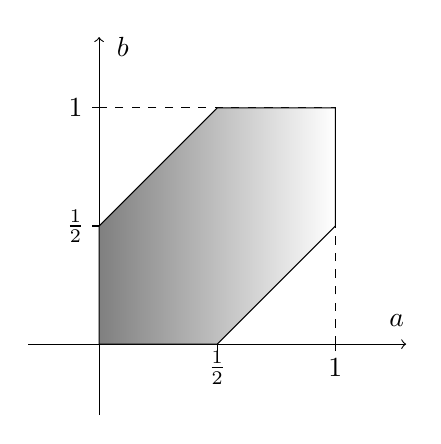
\begin{tikzpicture}[scale=3]
    \draw[->] (-0.3,0) -- (1.3,0) node at (1.26,0.1) {$a$};
    \draw[->] (0,-0.3) -- (0,1.3) node at (0.1,1.26) {$b$};;
    \draw (1,-0.03) -- (1,0.03);
    \draw (-0.03,1) -- (0.03,1);
    \draw (0.5,-0.03) -- (0.5,0.03);
    \draw (-0.03,0.5) -- (0.03,0.5);
    \draw[dashed] (1,0) -- (1,1) -- (0,1);
    \node at (1,-0.1) {$1$};
    \node at (-0.1,1) {$1$};
    \node at (0.5,-0.1) {$\frac{1}{2}$};
    \node at (-0.1,0.5) {$\frac{1}{2}$};
    \shadedraw[left color=gray,right color=white]  (0,0) -- (0.5,0) -- (1,0.5) -- (1,1) -- (0.5,1) -- (0,0.5) -- (0,0);
    \end{tikzpicture}
    \end{figure}
    Introducing the 3rd dimension, $|a-b|<\frac{1}{2}$ turns out to be an hexagonal prism (the base is shown above) whose height is 1 (along the c-axis). Similarly $|b-c| <\frac{1}{2}$ is the same solid, but rotated 90 degrees around the line parallel to the b-axis and going through the point($\frac{1}{2}$,$\frac{1}{2}$,$0$). Let's now compute the intersection between those solids, which turns out to be the sum of few smaller solids, in particular: 2 cubes with side $\frac{1}{2}$, 2 square pyramids with base length and height $\frac{1}{2}$ and 4 triangular prism, having height $\frac{1}{2}$ and an isosceles right triangle with side $\frac{1}{2}$ as base. Finally  the probability is $$\displaystyle p=\frac{2\cdot\frac{1}{8}+2\cdot\frac{1}{24}+4\cdot\frac{1}{8}}{1}=\frac{7}{12}$$ which leads to 712 as final answer.
\end{solution}\bigskip

        \newpage

        \subsubsection{Dividing Functions}
            \label{7.1.5}  
            \SSbreak\\
\emph{Source: \Cop}\\
\emph{Proposer: \Pchris}\\
\emph{Problem ID: 106}\\
\emph{Date: 2021-01-22}\\
\SSbreak

\SSpsetQ{
Find the smallest integer \(n > 1\) for which there exist positive integers \(a_1, a_2, \ldots,  a_n\)such that \[(a_1)^2 +\ldots + (a_n)^2 \big| \left[(a_1 + \cdots a_n)^2 - 1)\right]\]
}\bigskip

\begin{solution}[Solution by \Pchris]\hfil\medskip

    Note that squares are congruent to themselves\(\pmod 2\), so \[(a_1)^2 + \ldots + (a_n)^2 = a_1 +\ldots + a_n = (a_1 + \ldots + a_n)^2\pmod{2}\] Since \((a_1)^2 + \ldots + (a_n)^2\) divides \((a_1 +\ldots + a_n)^2 - 1\) which has a different parity, we must have the former odd and the latter even, so \((a_1 + \ldots + a_n)\) is odd. As all odd squares are \(1\mod 8\), \((a_1 +\ldots+ a_n)^2 - 1\) must be divisible by 8, and since \((a_1)^2 + \ldots+ (a_n)^2 \) is odd, we must have 
    \begin{equation*}
    \frac{(a_1 + \ldots + a_n)^2 - 1}{(a_1)^2 + \ldots + (a_n)^2} \geq 8
\end{equation*}
    Using Cauchy-Schwartz on the sequences \((a_1, \ldots, a_n)\) and \((1, 1, ..., 1)\) gives \[n((a_1)^2 + ... + (a_n)^2 \geq (a_1 + \ldots+ a_n)^2) > ((a_1 +\ldots + a_n)^2 - 1)\], which is a direct contradiction if \(n\) is less than 9. Therefore we must have \(n \geq 9\). It is easy to see \(n = 9\) works, with an example construction being \((1, 1, 1, 1, 1, 1, 1, 2, 2)\) which works as \(7*(1^2) + 2*(2^2) = 15\) and \((7*1 + 2*2)^2 - 1 = 120\), with \(120/15 = 8\) being an integer.\\

    \fbox{9}
\end{solution}\bigskip

        \newpage

        \subsubsection{Paper Monster}
            \label{7.1.6}  
            \SSbreak\\
\emph{Source: \Como 2013 P29}\\
\emph{Proposer: \Pchan}\\ 
\emph{Problem ID: 107}\\
\emph{Date: 2021-01-23}\\
\SSbreak

\SSpsetQ{

    After the TST the PSC meets Chrispi. \medskip

    Chrispi has $255$ sheets of paper, each labeled with a unique nonempty subset of ${1,2,3,4,5,6,7,8}$. Each minute, he chooses one sheet of paper uniformly at random out of the sheets of paper not yet eaten. \medskip
    
    Then, he eats that sheet of paper, and all remaining sheets of paper that are labeled with a subset of that sheet of paper (for example, if he chooses the sheet of paper labeled with ${1,2}$, he eats that sheet of paper as well as the sheets of paper with ${1}$ and ${2}$). \medskip
    
    The expected value of the number of minutes that Chrispi eats a sheet of paper before all sheets of paper are gone can be expressed in the form $\frac{m}{n}$, where $m$ and $n$ are relatively prime positive integers. Find $100m + n$.
    difficulty
}\bigskip

\begin{solution}\hfil\medskip
    
    \href{https://artofproblemsolving.com/community/c487h560346/20132014/fall/omo/29}{\SSaops}\\
    Answer: \fbox{20508}

\end{solution}\bigskip
        \newpage
        
        \subsubsection{Tan's Optimisation}
            \label{7.1.7}  
              
\SSbreak\\
\emph{Source: Cambridge Handout}\\
\emph{Proposer: \Ptan}\\
\emph{Problem ID: 108}\\
\emph{Date: 2021-01-24}\\
\SSbreak

\SSpsetQ{
    After Brainy and Yuchan placed joint first at the IMO, both perfect scoring, they decide to take the day off before going on a journey to replace .19 and add more people to the problem solving committee. As part of the recruitment process, they ask the following question to the applicants:\\
    
    Given that the  maximum value of \begin{equation*}
        \frac{x_1x_2+x_2x_3+\cdots+x_{20}x_{21}+x_{21}x_1}{x_1^2+\cdots+x^2_{21}}
    \end{equation*}
    is \(M\) for \(x_1+\cdots+x_{21}=0\), find  \(\floor{1000M}\)\\
    
    What answer should the applicants put down?\bigskip
    
    \begin{center}
    \emph{(A scientific calculator may be used)}
    \end{center}
}\bigskip

\begin{solution}[Solution by \Ptan]\hfil\medskip
	
We will prove it for a given $n$, here $n = 21$. \medskip

Let $\omega$ be the principle $n$th root of unity. \medskip

Let $$y_k = \frac1{\sqrt n} \sum_{i=1}^n x_i \omega^k. $$ \medskip

Note that $$|y_1|^2 + |y_2|^2 + \cdots + |y_k|^2 = |x_1|^2 + |x_2|^2 + \cdots + |x_k|^2$$ and $$x_1 x_2 + \cdots + x_n x_1 = \frac 1 n \sum_{k=1}^n (\omega^k + \omega^{-k})y_k^2$$

Since $x_1 + \cdots + x_n = 0$, we get $y_n = 0$, so the sum is maximised when $y_{n-1}$ or $y_1$ is maximal since $k=1, n-1$ are the values where $\omega^k + \omega^{-k}$ is the biggest and that gives $2 \cos(\frac{2\pi}n)$. 
\end{solution}\bigskip

        \newpage
        
	\ihead{\footnotesize\bfseries\sffamily{PSC's Adventure (Season 7), Week 2}}
    \subsection{Week 2}
        
        \subsubsection{A Digital Product equal to Half the Number}
        	\label{7.2.1}  
        	\SSbreak\\
\emph{Source: \Cfolk}\\
\emph{Proposer: \Pss}\\
\emph{Problem ID: 110}\\
\emph{Date: 2021-01-25}\\
\SSbreak

\SSpsetQ{
  AiYa claims that he has found the smallest two-digit positive integer with the property that when divided by two, it is equal to the product of its digits.  \medskip

Assuming AiYa is correct, what number has he found?\bigskip

  \begin{center}
      \emph{(If needed, a four-function calculator may be used)}
  \end{center}
}\bigskip

\begin{solution}\hfil\medskip

  Let the integer have digits \(x\) and \(y\). We require:
  \begin{align*}
    xy=&\frac{10x+y}{2}\\
    2xy-10x-y&=0\\
    2xy-10x-y+5&=5\\
    (2x-1)(y-5)&=5
  \end{align*}
Since 5 is prime, it has factors of either 1 or 5. Hence we have either \(y-5=5\) or \(y-5=1\). We don't need to consider negatives as it's clear \(x\) would not be positive (and non-zero). We see that \(y=6\), as in the other case, \(y>9\). THis means that \(2x-1=5\), giving \(x=3\). So the answer is \(\fbox{36}\)
\end{solution}\bigskip

        \newpage
        
        \subsubsection{Unique Odd Numbers}
        	\label{7.2.2}  
        	  \SSbreak\\
\emph{Source: \Cfolk}\\
\emph{Proposer: \Pkiesh}\\ %\Pchan \Pbrain \Pss
\emph{Problem ID: 112}\\
\emph{Date: 2021-01-26}\\
\SSbreak

\SSpsetQ{
    Call a number unique if each of its digits are unqiue (no two are the same). How many odd integers in the interval \([3\cdot10^4,8\cdot10^4]\) are unique?\medskip

    \begin{center}
        \emph{(A four-function calculator may be used)}
    \end{center}
}\bigskip

\begin{solution}\hfil\medskip

There are 5 ways to choose the first digit. If the first digit is odd, then we must consider the final digit too. In the even cases, there are 2 numbers to choose from for the first digit, then last digit we have 5 odd digits to choose from. Then for the other 3 digits, we have 7! ways to pick digits, so there are \(2\cdot5\cdot\frac{8!}{5!}\) ways when the first digit is even. When it is odd, however, there is one less odd digit to choose from for the last digit. There are 3 ways to choose the first digit and 4 ways to choose the last digit. As before there are \(\frac{8!}{5!}\) ways to choose the middle three digits. This gives us a total of \(3\cdot4\cdot\frac{8!}{5!}\) when the first digit is odd.

Thus in total, there are \(2\cdot5\cdot\frac{8!}{5!}+3\cdot4\cdot\frac{8!}{5!}=\fbox{7392}\)
\end{solution}\bigskip

        \newpage

        \subsubsection{Maximising \(a^4+b^4\)}
            \label{7.2.3}  
            \SSbreak\\
\emph{Source: \Cfolk}\\
\emph{Proposer: \Pss}\\
\emph{Problem ID: 111}\\
\emph{Date: 2021-01-27}\\
\SSbreak

\SSpsetQ{
Let \(a^2-ab+b^2\geq15\) for \(a,b\in\R\). What is the maximum value of \(a^4+b^4\)?
}\bigskip

\begin{solution}\hfil\medskip

Notice that \(a^4+b^4=(a^2+b^2)^2-2(ab)^2\). Thus, \(a^4+b^4\leq (2+ab)^2-2(ab)^2\) - this is simply a quadratic in \(ab\).\\

Therefore, we have, by \emph{the method of maximising a quadratic of your choosing}

\begin{equation*}
  a^4+b^4\leq 450-(ab-2)^2
\end{equation*}
So our answer is \fbox{450}.
\end{solution}
        \newpage    

        \subsubsection{Minimising Perimeter}
            \label{7.2.4}
            \SSbreak\\
\emph{Source: China Mathematical Competition (Extra Test), 2003 P2}\\
\emph{Proposer: \Pss}\\
\emph{Problem ID:}\\
\emph{Date: }\\
\SSbreak

\SSpsetQ{
Find the \textbf{minimum} perimeter of a triangle having integer sides $a > b > c > 0$, such that $$\frac{3^a}{10^4}-\floor{\frac{3^a}{10^4}} = \frac{3^b}{10^4}-\floor{\frac{3^b}{10^4}} = \frac{3^c}{10^4}-\floor{\frac{3^c}{10^4}},$$ where $\floor{x}$ denotes the greatest integer less than or equal to $x$, e.g. $\floor{\pi} = 3$, and so on.
}\bigskip

\begin{solution}\hfil\medskip

Note that this condition implies $l \equiv m \equiv n \pmod{(\ord_{10000}(3)}$. Let us calculate $\ord_{10000}(3)$. \medskip

By LTE, $\nu_2(3^n -1) = \nu_2(3-1) + \nu_2(n) + \nu_2(3+1) - 1 = \nu_2(n) + 2$, and so if $3^n \equiv 1 \pmod 2^4$ we must have $\nu_2(n) \ge 2$, implying that $n \ge 4$ and so $\ord_{2^4}(3) = 4$. \medskip

By LTE again, note that $\nu_5(81^n - 1) = \nu_5(81 - 1) + \nu_5(n) \ge 4$. Hence we must have $\nu_5(n) \ge 3$ which implies $n \ge 125$. Since $81 = 3^4$ we get that $\ord_{5^4}(3) = 500$. \medskip

Now $\ord_{10^4}(3) = \lcm(\ord_{2^4}(3), \ord_{5^4}(3)) = 500$. \medskip

Hence for our minimum we must have $l = n + 1000, m = n + 500$. Since they are the sides of a triangle $l < m + n \implies n + 1000 < 2n + 500 \implies n > 500$. So $n = 501$ and so the smallest value of $l+m+n$ is $1501 + 1001 + 501 = \boxed{3003}$. 
\end{solution}

        \newpage 

        \subsubsection{Binary Blocks}
            \label{7.2.5}  
              
\SSbreak\\
\emph{Source: Harvard-MIT Math Tournament, 2015 C5}\\
\emph{Proposer: \Pchan}\\
\emph{Problem ID: 116}\\
\emph{Date: 2021-01-29}\\
\SSbreak

\SSpsetQ{
  One night while sleeping, Brainy has a vision that the entirety of the new PSC has been found, and that they must now return to the jungle to find their mysterious advisor who will lead them out of this dimension. \medskip

  The next day, Brainy picks up everybody, but is stopped at Yuchan's house by MODSbot, who plans to trap the PSC in this dimension. \medskip
  
  To distract it, Brainy orders MODSbot to write out every integer from $1$ to $256$ in binary, with a space between each. It takes MODSbot $1$ minute to write each unbroken block of $1$s and a negligible amount of time to write $0$s and spaces. \medskip
  
  How long in minutes does Brainy have to collect the rest of the PSC and escape the city?
}\bigskip

\begin{solution}\hfil\medskip
  
  Define $g(0) = 0$. Call a digit of a number represented in binary "good" if it is $1$ and the preceding digit is $0$. Then $g(0)+ g(1) + g(2) + ... + g(255)$ is $256 E(X_8)$ where $E(X_8)$ is the expected value of the number of "good" digits given that the number is less than $2^8$. 

  By linearity of expectation, the expected number of good digits is $E(X_8) = E(G_1)+E(G_2) + ... + E(G_8)$ where $G_i$ is defined as 
  \begin{equation*}
      \begin{cases}
      1 & \text{if the $i$th digit from the back is good}\\
      0 & \text{otherwise}
      \end{cases}
  \end{equation*}
  For example, $G_3$ for $7$ would be $1$ but $G_2$ for $7$ would be $0$ since there is already a $1$ before that. Then we can find $E(G_i) = \frac14$ for all $i = 1,2,3,4,5,6,7$ since its just $\frac 12$ chance that the $i$th digit is $1$ multiplied by $\frac 12$chance that the preceding digit is $0$. However, $E(G_8) = \frac 12$ since the preceding digit is guaranteed to be $0$, from which we can find $E(X_8) = \frac 12 + 7 \frac 14 = \frac 94$

Thus $g(0)+ g(1) + g(2) + \ldots + g(255) = 256 \cdot \frac94$ and $g(1) + g(2) + \ldots + g(255) + g(256) = \fbox{577}$.
\end{solution}\bigskip

\begin{solution}[Solution by \Prishi]\hfil\medskip

  Let's say the bot's done printing until $n-1$ digits. Now let us append a digit.\\
We see that the bot will have to print all the numbers it has printed again so that one set of it can be appended with $0$ and the other with $1$. This takes exactly twice the amount of time taken for $(n-1)$ digits.\\

Whenever the ending digit was a $0$ and the appended digit a $1$. The bot takes a minute more to print it. It can be seen from some combinatorics that no. of numbers of $(n-1)$ digit numbers ending with 0 is exactly ${2 \choose 1}^{n-2} \cdot 1$ and one resulting number appended with $1$ for each of those.\\

Thus the recurrence is:
$$t_n = 2t_{n-1} + 2^{n-2}$$
$1$ to $256$ would be all 8 digit strings of 1 or 0 along with the number $100000000$.
Thus the time Bot takes is:
$$t_8+1$$
It can be seen that:
$$t_n = 2^k t_{n-k} + k\cdot 2^{n-2} \ ; \ t_1 = 1$$
$$t_8+1 = \fbox{577}$$
\end{solution}
        \newpage

        \subsubsection{Funkey Triangles}
            \label{7.2.6}  
            \SSbreak\\
\emph{Source: \Cop}\\
\emph{Proposer: \Pmatt}\\
\emph{Problem ID: 117}\\
\emph{Date: 2021-01-30}\\
\SSbreak

\SSpsetQ{
    Having successfully gathered the PSC and escaped the scheming MODSbot, Brainy manages to lead the group to the jungle. Not far into the jungle, they meet Tan, who tells them that he is their mysterious advisor. He also says that he needs to take them to the last remaining population of wild triangles. \medskip

    Some of the triangles are a deep shade of red; Tan explains that a triangle $\triangle ABC$ is red if given its incenter $I$, points $B_1$ and $C_1$ the intersections of $BI$ and $CI$ with $AC$ and $AB$ and $P$, $Q$ the intersections of line $PQ$ with $(ABC)$, $\angle PIQ$ attains the minimal possible value over all acute triangles. Each red triangle has upon its face the value of $\cos(\angle BAC)$. \medskip
    
    If the product of all numbers written on any triangle in the population for which $AB=AC$ can be written in the form $a - b\sqrt{c}$, where $a$, $b$, $c$ are positive integers with $c$ squarefree, find $10000a+100b+c$.
 
}\bigskip

\begin{solution}[Solution by \Pmatt]\hfil\medskip

Let $I_b$ and $I_c$ be the excenters opposite $B$ and $C$ respectively. Since $IAI_cB$ is cyclic, we have $C_1A \cdot C_1B=C_1I \cdot C_1I_c$, which implies $C_1$ lies on the radical axis of $(ABC)$ and $(I_bII_c)$, and so does $B_1$. This means that $B_1C_1$ is the radical axis of those circles, which implies that $P$ and $Q$ are their intersection points. Since $(ABC)$ is the Feuerbach circle of $\triangle I_bII_C$, the radius of $(I_bII_C)$ is twice that of $(ABC)$ for all triangles, which means that the minimal value of $\angle PIQ$ happens when $PQ$ is maximised, so when it is a diameter, and in this case it's easy to see $\angle PIQ=150^{\circ}$. Now consider the case when $\triangle ABC$ is funky and isosceles, and let $O$ be the circumcenter, $M$ be the midpoint of arc $BC$ in $(ABC)$ and suppose the radius of $(ABC)$ is $1$. Then $2Rsin(\angle MAB)=MB=MI=R\pm OI=R(1\pm tan(15^{\circ}))$, which gives the possible values of $\cos\left(\angle BAC\right)$ to be $\sqrt{3}-1$ and $3\sqrt{3}-5$, and their product is $14-8\sqrt{3}$. This therefore gives us an answer of \(\fbox{336}\)
\end{solution}\bigskip

        \newpage

        \subsubsection{A Lotta Touples!}
            \label{7.2.7}  
            \SSbreak\\
\emph{Source: \Cctst 4 2017, P3}\\
\emph{Proposer: \Pmatt}\\
\emph{Problem ID: 115}\\
\emph{Date: 2021-01-31}\\
\SSbreak

\SSpsetQ{
    Having successfully gathered the PSC and escaped the scheming MODSbot, Brainy manages to lead the group to the jungle. Not far into the jungle, they meet Tan, who tells them that he is their mysterious advisor. He also says that he needs to take them to the last remaining population of wild triangles. \medskip

Some of the triangles are a deep shade of red; Tan explains that a triangle $\triangle ABC$ is red if given its incenter $I$, points $B_1$ and $C_1$ the intersections of $BI$ and $CI$ with $AC$ and $AB$ and $P$, $Q$ the intersections of line $PQ$ with $(ABC)$, $\angle PIQ$ attains the minimal possible value over all acute triangles. Each red triangle has upon its face the value of $\cos(\angle BAC)$. \medskip

If the product of all numbers written on any triangle in the population for which $AB=AC$ can be written in the form $a - b\sqrt{c}$, where $a$, $b$, $c$ are positive integers with $c$ squarefree, find $10000a+100b+c$.
}\bigskip

\begin{solution}\hfil\medskip

\href{https://artofproblemsolving.com/community/c6h1408832p7904039}{\SSaops}

Answer: \fbox{197666}
\end{solution}\bigskip

        \newpage
        
\ihead{\footnotesize\bfseries\sffamily{A New Chapter (Season 8)}}
\section{A New Chapter (Season 8)}
        
    \ihead{\footnotesize\bfseries\sffamily{A New Chapter (Season 8), Week 1}}
    \subsection{Week 1}

        \subsubsection{Smallest Non-Factor}
            \label{8.1.1}
            \SSbreak\\
\emph{Source: \Csmc 1999 Q9}\\
\emph{Proposer: \Pss}\\
\emph{Problem ID: 119}\\
\emph{Date: 2021-02-01}\\
\emph{Difficulty: Beginner}\\
\SSbreak
 
\SSpsetQ{
    Let \(N=50!\). What is the smallest positive integer which does not divide \(N\)?
}\bigskip

\begin{solution}\hfil\medskip
  
The question can be rephrased as '\emph{what is the smallest prime number greater than 50}'. To which the answer is \fbox{53}
\end{solution}\bigskip

        \newpage
        
        \subsubsection{Product of Radii}
            \label{8.1.2}  
            \SSbreak\\
\emph{Source: \Csmc 2003 Q24}\\
\emph{Proposer: \Pss}\\
\emph{Problem ID: 120}\\
\emph{Date: 2021-02-02}\\
\emph{Difficulty: Beginner}\\
\SSbreak

\SSpsetQ{
Let \(AOB\) be an isosceles right-angled triangle drawn in a quadrant of a circle of radius unit 1. The largest possible circle drawn in the minor segment cut by the line \(AB\) has radius \(r\). The radius of the inscribed circle of the triangle \(AOB\) is \(R\). Given that the value of \(Rr\) can be written in the form \(\frac{a - b\sqrt{c}}{d}\), where \(a,b,c,d\) are positive integers and \(c\) is square-free.\medskip

What is the value of \(a^2 + b^2 + c^2 + d^2\)?
}\bigskip

\begin{solution}\hfil\medskip

\begin{figure}[h!]
    \centering
    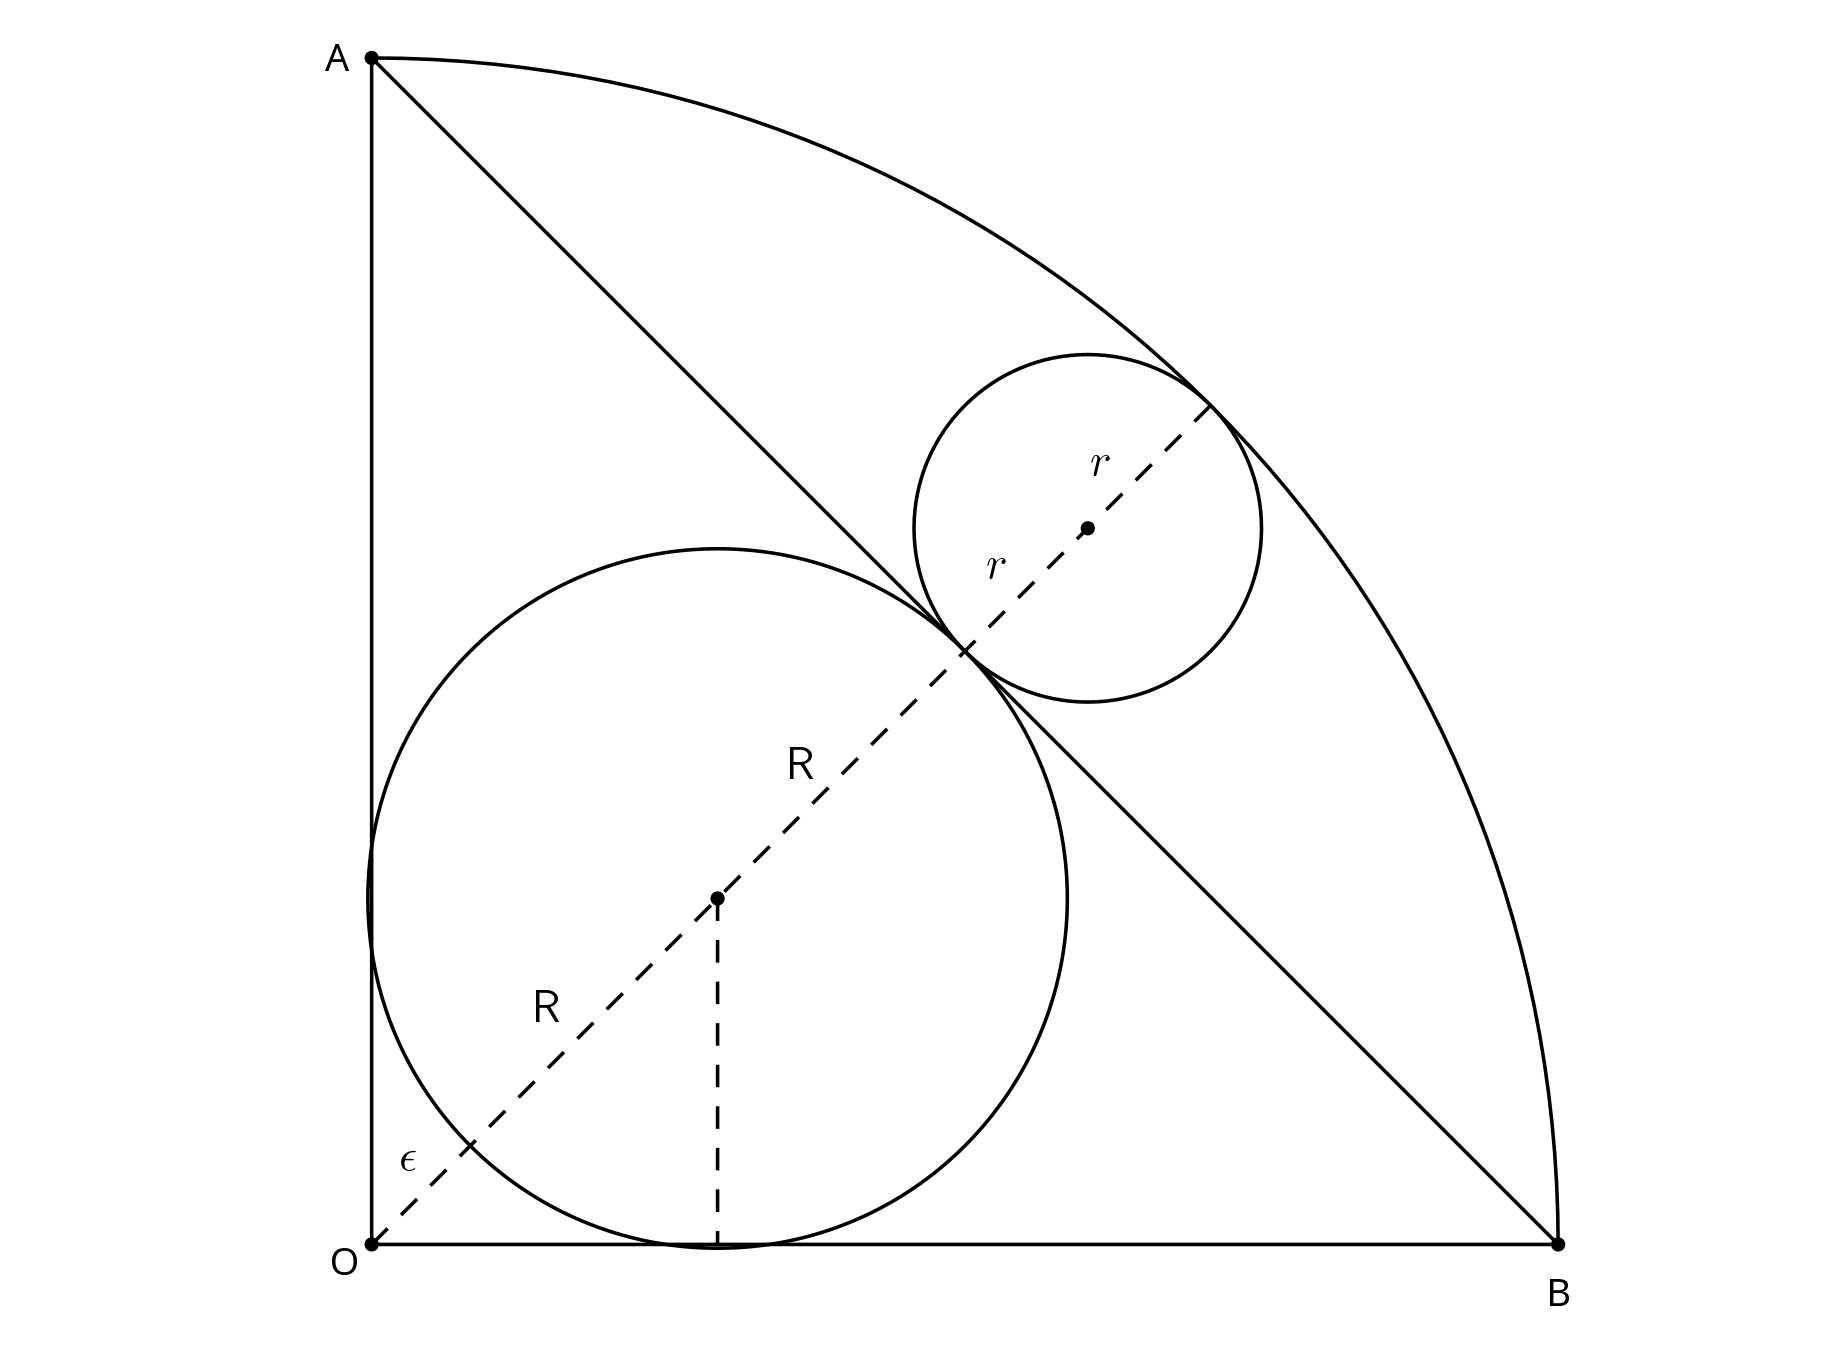
\includegraphics{Sections/Files/SMC-2003-Q24}
\end{figure}
Observe that \(\epsilon + 2R + 2r = 1\) and \(\epsilon + 2R = \frac{1}{\sqrt{2}}\), therefore we have \(r = \frac{\sqrt{2}-1}{2\sqrt{2}}\). Then by the sine rule, \(\frac{\sin(45)}{R} = \frac{\sin(90)}{R + \epsilon}\Rightarrow R = \frac{1}{\sqrt{2} + 2}\), this gives \(Rr = \frac{3 - 2\sqrt{2}}{4}\), hence our answer is \(3^2 + 2^2 + 2^2 + 4^2 = \fbox{33}\)
\end{solution}\bigskip

        \newpage

        \subsubsection{Two-to-One Functions}
            \label{8.1.3}  
            \SSbreak\\
\emph{Source: \Cfolk}\\
\emph{Proposer: \Pss}\\
\emph{Problem ID: 121}\\
\emph{Date: 2021-02-03}\\
\emph{Difficulty: Easy}\\
\SSbreak

\SSpsetQ{
Define a function \(f:\{1,2,\ldots,12\}\to\{1,2,\ldots,6\}\) such that for every \(y\in \{1,2,\ldots,6\}\) there exists exactly two elements \(x_1,x_2\in \{1,2,\ldots,12\}\) such that \(f(x_1)=f(x_2)=y\). How many such functions are there which map \(\{1,2,\ldots,12\}\) to \(\{1,2,\ldots,6\}\) with the described property?

\begin{center}
  \emph{(A four-function calculator may be used)}
\end{center}
}\bigskip

\begin{solution}\hfil\medskip

This well known property can be derived simply by considering how we can choose two elements in \(\{1,2,\ldots,12\}\) and enumerating that. Let the number of such functions be \(F\), then we have:
\begin{align*}
  F&=\prod_{i=1}^{12}\binom{2i}{2}\\
  &=\frac{12!}{2^6}\\
  &=\fbox{7484400}\ \mathrm{such\ functions}
\end{align*}
\end{solution} 
        \newpage

        \subsubsection{Modular Powers}
            \label{8.1.4}  
              
\SSbreak\\
\emph{Source: New Zealand Mathematical Olympiad Round 1, 2019 Q4 (Adapted)}\\
\emph{Proposer: \Pbrain }\\ %\Pchan \Pbrain \Pss
\emph{Problem ID: 122}\\
\emph{Date: 2021-02-04}\\
\emph{Difficulty: Medium}\\
\SSbreak

\SSpsetQ{
	Find the remainder when \(122^{2020} - 102^{2020} - 21^{2020}\) is divided by 2020. 
	%Put Problem Here
}\bigskip

\begin{solution}\hfil\medskip
	
	Let \(X = 122^{2020} - 102^{2020} - 21^{2020}\). \\
	Note that \(2020 = 20 \times 101\). In particular, considering the expression mod 20 we get \(X = 2^{2020} - 2^{2020} - 1^{2020} \equiv -1 \pmod{20}\), and considering it mod 101 we get \(X = 21^{2020} - 1^{2020} - 21^{2020} \equiv -1 \pmod{101}\). \\
	In particular, by Chinese Remainder Theorem we get \(X \equiv -1 \pmod{2020}\) which means that the remainder on division by 2020 of \(X\) is \(\boxed{2019}\). \\
	\emph{Note: The choice of 2020 in the exponent is not special.}
	%Put sol here
\end{solution}\bigskip

        \newpage

        \subsubsection{Australian Nim}
            \label{8.1.5}  
            \SSbreak\\
\emph{Source: AMO 2020 P2}\\
\emph{Proposer: \Pchris}\\ 
\emph{Problem ID: 123}\\
\emph{Date: 2021-02-05}\\
\emph{Difficulty: Medium}\\
\SSbreak

\SSpsetQ{
sjbs and Brainy are playing a game. First, they'll use a random number generator to generate three random positive integers. Then, three piles of stones will magically appear before them; the number of stones in each pile are the numbers generated previously. Then they'll take turns, with sjbs going first. On a player's turn, they can pick one pile and split it into either two or three nonempty piles, throwing the rest of the stones in the other two piles away. The game ends when a player can't make a move. Suppose both players play perfectly like the smart people they are - then if the probability that sjbs wins is \(m/n\), with \(gcd(m, n) = 1\) and \(m, n\) positive integers, find \(m + n\).
}\bigskip

\begin{solution}\hfil\medskip

Call a pile \textit{perilous} if it contains a number of stones equal to $3k + 1$ where $k$ is a nonnegative integer and \textit{safe} otherwise. I claim that a player can force a win, if at their turn they have at least one safe pile in front of them, and lose otherwise. 
Note that from a safe pile, the turn player can always give the other player either 2 or 3 perilous piles: simply consider splitting a pile of stones equal to $3k + 2$ into two piles, one of 1 stone and 1 of $3k + 1$ stones, which are both perilous, or a pile equal to $3k$ stones into three piles, two of 1 stone and 1 of $3k - 2 = 3(k - 1) + 1$ stones which are all perilous. Also note that from a perilous pile, it is impossible to leave only perilous piles behind, since two or three perilous piles imply that the original split pile was safe. \medskip

So if a player has at least one safe pile in front of them on their turn, they may make two or three perilous piles; then their opponent must return them at least one safe pile and they can repeat this; noting that the total number of stones in game is strictly decreasing so the game must end and that the losing state (all piles with 1 stone) is all perilous piles shows that they will win. And clearly if a player only has perilous piles before them then they must give their opponent at least one safe pile and thus their opponent wins. 
Thus sjbs wins if at least one of the three piles generated at the start is safe, and brainy wins if they are all perilous. The probability of brainy's win is thus $\frac{1}{3} \cdot \frac{1}{3} \cdot \frac{1}{3} = \frac{1}{27}$ so the probability sjbs wins is $1 - \frac{1}{27} = \frac{26}{27}$ and so the answer is $26 \cdot 100 + 27 = \boxed{2627}$.
\end{solution}\bigskip

        \newpage

        \subsubsection{Another Geo Config}
            \label{8.1.6}  
            \SSbreak\\
\emph{Source: Italian Team Competition Final 2020}\\
\emph{Proposer: \Pmatt}\\ 
\emph{Problem ID: 124}\\
\emph{Date: 2021-02-06}\\
\emph{Difficulty: Challenging}\\
\SSbreak

\SSpsetQ{
For a triangle \(ABC\), let \(P\) be on \(AB\), and \(X\) be the circumcenter of \(APC\), \(Y\) be the circumcenter of \(BPC\), and \(Z\) be the intersection of \(AX\) and \(BY\). Given that \(AB=91\), \(BC=104\), and \(CA=65\), what is the length of \(CZ\)?
}\bigskip

\begin{solution}\hfil\medskip

    \begin{figure}[h!]
        \centering
    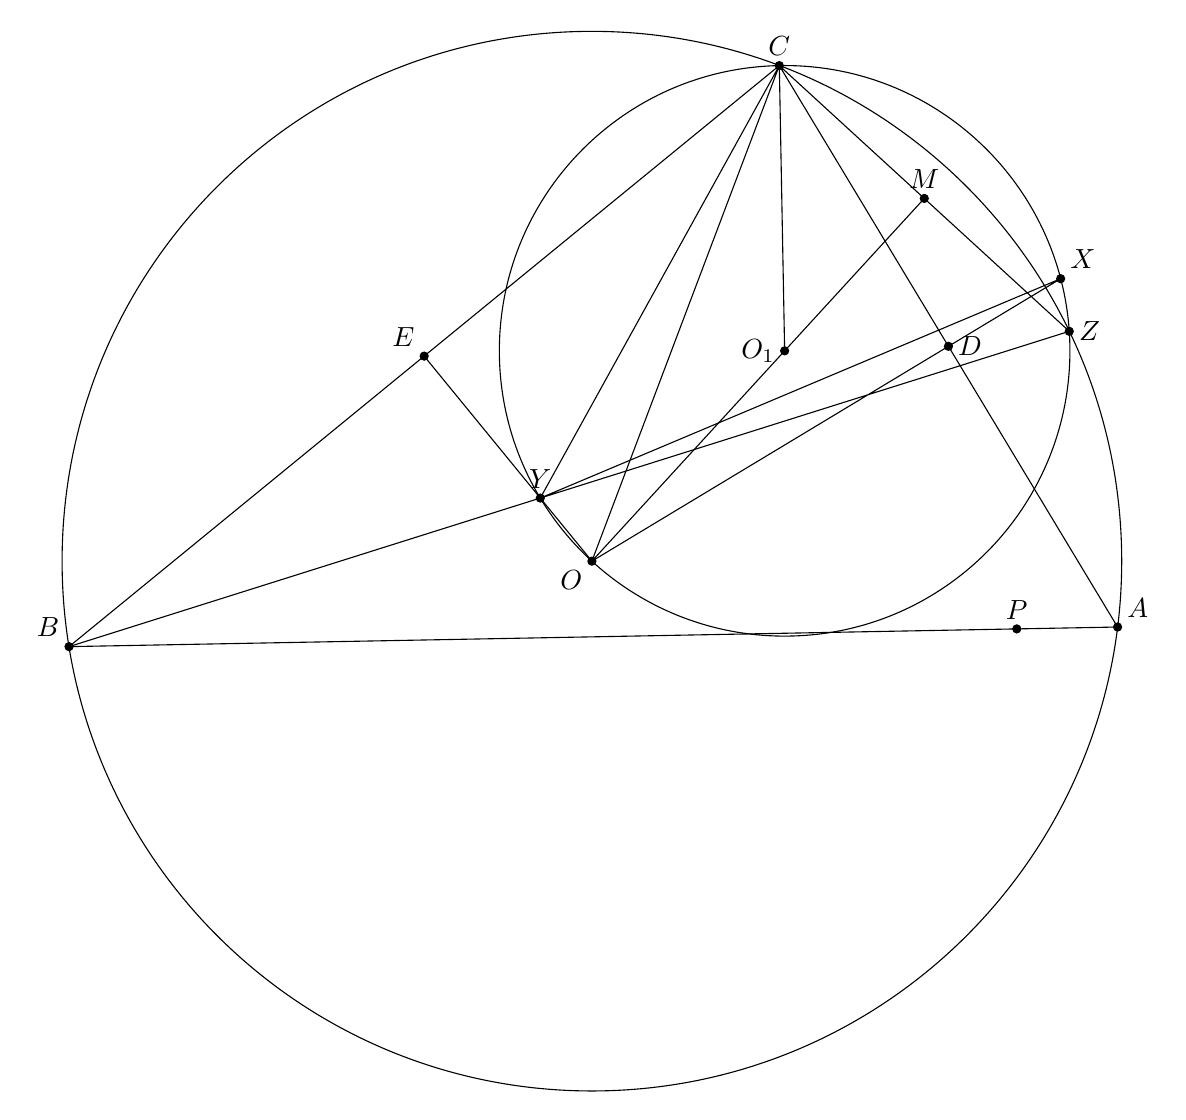
\begin{tikzpicture}[scale = 0.0045cm]
    \def\A{(-73.1687,-160.74487)}
    \def\B{(-177.150601,-162.690109)} 
    \def\C{(-106.716,-105.07095)}
    \def\P{(-83.167045,-160.931914)} 
    \def\Y{(-130.41799645,-147.9570)} 
    \def\Z{(-77.96303196,-131.419898)} 
    \def\O{(-125.3000,-154.21325)}
    \def\X{(-78.81585,-126.20343707)}
    \def\o{(-106.186855,-133.356169)} 
    \def\M{(-92.33951608,-118.2454)} 
    \def\D{(-89.94239,-132.9079)}
    \def\E{(-141.9333,-133.880532)}
    \filldraw \B circle (0.4) node[above left] {$B$}; %B
    \filldraw \A circle (0.4) node[above right] {$A$}; %A
    \filldraw \C circle (0.4) node[above] {$C$}; %C
    \filldraw \X circle (0.4) node[above right] {$X$}; %X
    \filldraw \P circle (0.4) node[above] {$P$}; %P
    \filldraw \Y circle (0.4) node[above] {$Y$}; %Y
    \filldraw \Z circle (0.4) node[right] {$Z$}; %Z
    \filldraw \O circle (0.4) node[below left] {$O$}; %O
    \filldraw \o circle (0.4) node[left] {$O_1$}; %o
    \filldraw \M circle (0.4) node[above] {$M$}; %M
    \filldraw \D circle (0.4) node[right] {$D$}; %D
    \filldraw \E circle (0.4) node[above left] {$E$}; %E
    \draw (-125.3000,-154.21325) circle (52.53887);
    \draw (-106.186855,-133.356169) circle (28.29016);
    \draw \E -- \B -- \A -- \C -- \E -- \Y -- \C  -- \Z -- \Y -- \X -- \O -- \C -- \o;
    \draw \B -- \Y -- \O -- \M;
    \end{tikzpicture}
    \end{figure}


    By simple angle chasing $\triangle CXA$ and $\triangle CYB$ are similar, we have $\angle ZAC=\angle XAC=\angle YBC=\angle ZBC$, so $Z$ is on $\odot (ABC)$. Standard calculations on $\triangle ACX$ and $\triangle ABC$ give $\text{sin}(\angle ZAC)=\frac{3\sqrt{3}}{14}$ and $R_{\odot (ABC)}=\frac{91\sqrt{3}}{3}$, so $CZ= 2R_{\odot (ABC)}\text{sin}(\angle ZAC)=39$
\end{solution}\bigskip

        \newpage

        \subsubsection{Product of Root Differences}
            \label{8.1.7}  
            \SSbreak\\
\emph{Source: Original}\\
\emph{Proposer: \Ptan}\\ %\Pchan \Pbrain \Pss
\emph{Problem ID: 125}\\
\emph{Date: 2021-02-07}\\
\emph{Difficulty: Challenging}\\
\SSbreak

\SSpsetQ{
	Let $\alpha_1, \alpha_2, \dots, \alpha_{2021}$ be the roots of $x^{2021} + 20x^2 + 21$. Find \[\prod_{1 \le i < j \le 2021} (\alpha_i - \alpha_j)\]
	%Put Problem Here
}\bigskip

\begin{solution}[Write up by \Ptroll]\hfil\medskip
	
	We solve for general $f(x) = x^n + ax^2 + b$, where $n \equiv 1 \pmod{4}$. Let $P$ be our product, we have 
	$$P = \prod_{i < j}\left(\alpha_i - \alpha_j\right)^2 = \prod_{i \neq j}\left(\alpha_i - \alpha_j\right)$$
	since we flipped the signs of $\sum_{k = 1}^{n - 1}k \equiv 0 \pmod{2}$ factors. Fix $i$; our product becomes
	$$P = \prod_{i = 1}^n \prod_{j \neq i} \left(\alpha_i - \alpha_j\right) 
	= \prod_{i = 1}^n \dfrac{\prod_{j = 1}^n \left(\alpha_i - \alpha_j\right)}{\alpha_i - \alpha_i} 
	= \prod_{i = 1}^n \dfrac{f\left(\alpha_i\right)}{\alpha_i - \alpha_i}$$
	after writing $x^n + ax^2 + b = \prod_{i = 1}^n \left(x - \alpha_i\right)$. Although division by zero is undefined, since polynomials are continuous functions
	we can use L'Hopital's Rule to write the product as a limit, then use calculus to get
	$$P = \prod_{i = 1}^n \lim_{x \to \alpha_i} \dfrac{f(x)}{x - \alpha_i} = \prod_{i = 1}^n n\alpha_i^{n - 1} + 2a\alpha_i 
	= -b n^n \prod_{i = 1}^n \left(\alpha_i^{n - 2} + \dfrac{2a}{n}\right).$$
	Let $\omega$ be a primitive $(n - 2)^\text{nd}$ root of unity and $r = \left(\frac{2a}{n}\right)^{\frac{1}{n - 2}}$. The roots of 
	$x^{n - 2} + r^{n - 2}$ are $-r\omega^k$ where $0 \leq k < n - 2$, so we can rewrite our product as
	$$P = -bn^n \prod_{i = 1}^n \prod_{j = 0}^{n - 2} \left(\alpha_i + r \omega^j\right) = -bn^n\prod_{j = 0}^{n - 2} \prod_{i = 1}^n \left(\alpha_i + r \omega^j\right)
	= bn^n\prod_{j = 0}^{n - 2} \prod_{i = 1}^n \left(-r \omega^j - \alpha_i\right) = bn^n \prod_{j = 0}^{n - 2} f\left(-r \omega^j\right).$$
	The rest is just computation.
	\begin{align*}
		P &= bn^n \prod_{j = 0}^{n - 2} \left(- r^n \omega^{jn} + ar^2 \omega^{2j} + b\right) = bn^n \prod_{j = 0}^{n - 2} \left[r^2 \omega^j \left(-r^{n - 2} + a\right) + b\right] \\
		&= bn^2 \prod_{j = 0}^{n - 2} \left[r^2 \omega^j a (n - 2) + bn\right] = bn^2 \left[r^{2(n - 2)} a^{n - 2} (n - 2)^{n - 2} + bn^{n - 2}\right] \\
		&= 4a^nb(n - 2)^{n - 2} + bn^n \\
		&\equiv \boxed{821} \pmod{10000}
	\end{align*}
\end{solution}\bigskip

\begin{solution}[Write up by \Paiya]\hfil\medskip

	Recall the fundamental theorem of symmetric polynomials: \textit{every symmetric polynomial of $n$ variables can be written as a function of the $n$-variable elementary symmetric polynomials.}
	Since $P = \prod_{i \neq j} \left(\alpha_i - \alpha_j\right)$ is symmetric in $n$ variables and all elementary symmetric polynomials in $n$ variables
	are zero except for $e_{n - 2}\left(\alpha\right) = -a$ and $e_n\left(\alpha\right) = -b$ (where $e_k(\alpha)$ is the $k$-th elementary symmetric sum), $P$ can be written as a sum of $(-a)^x(-b)^y$.
	$P$ has degree $n(n - 1)$, $-a$ has degree $n - 2$, and $-b$ has degree $n$ so we solve $(n - 2)x + ny = n(n - 1)$ to find our suitable powers of $-a$ and $-b$.
	Solving, we get $(x, y) = (n, 1); (0, n - 1)$ so $P = Qa^nb + Rb^{n - 1}$. It remains to choose easy $a, b$ to find $P, Q$; an obvious choice is $(a, b) = (0, 1)$
	and we have $$P = \prod_{i = 1}^n n \alpha_i^{n - 1} = n^n \iff R = n^n.$$ To find $Q$, we plug in $(a, b) = (1, 1)$ and since 
	$\alpha^n + \alpha^2 + 1 = 0 \iff \alpha^{n - 2} = - 1 - \frac{1}{\alpha^2}$ we have
	$$P = -\prod_{i = 1}^n \left(n \alpha_i^{n - 2} + 2\right) = - \prod_{i = 1}^n \left[(2 - n) - \dfrac{n}{\alpha_i^2}\right] = - \sum_{k = 0}^n (2 - n)^{n - k}(-n)^k e_k\left(\dfrac{1}{\alpha^2}\right).$$
	We first calculate $e_k\left(\frac{1}{\alpha}\right)$; from substituting $x \to \frac{1}{x}$ into $f(x)$ we get 
	$e_2\left(\frac{1}{\alpha}\right) = 1, e_n\left(\frac{1}{\alpha}\right) = -1$, $e_k = 0$ otherwise except for $e_0 = 1$ as convention. We solve for $e_1\left(\frac{1}{\alpha^2}\right)$ as follows:
	$$e_1^2\left(\dfrac{1}{\alpha}\right) = e_1\left(\dfrac{1}{\alpha^2}\right) + 2e_2\left(\dfrac{1}{\alpha}\right) \iff e_1\left(\dfrac{1}{\alpha^2}\right) = -2$$
	and similarly
	$$e_2^2\left(\dfrac{1}{\alpha}\right) = e_2\left(\dfrac{1}{\alpha^2}\right) + 2e_4\left(\dfrac{1}{\alpha}\right) + 2e_1\left(\dfrac{1}{\alpha^2}\right)e_2\left(\dfrac{1}{\alpha}\right) = 1.$$
	For larger values of $k$, note that 
	$$e_k^2\left(\dfrac{1}{\alpha}\right) = e_k\left(\dfrac{1}{\alpha^2}\right) + 2 \sum_{j = 0}^{k} e_j\left(\dfrac{1}{\alpha^2}\right)e_{2(k - j)}\left(\dfrac{1}{\alpha}\right)$$
	so all of them evaluate to zero except for $e_n\left(\frac{1}{\alpha^2}\right) = 1$. The rest is computation.
	\begin{align*}
		P &= (n - 2)^n - 2n(n - 2)^{n - 1} + n^2(n - 2)^{n - 2} + n^n \\
		&= (n - 2)^{n - 2}\left(n^2 - 4n + 4 - 2n^2 + 4n + n^2\right) + n^n \\
		&= 4(n - 2)^{n - 2} + n^n \iff P = 4(n - 2)^{n - 2} \\
		P &= 4a^nb(n - 2)^{n - 2} + b^{n - 1}n^n \\
		&\equiv \boxed{821} \pmod{10000}
	\end{align*}
\end{solution}\bigskip
        \newpage


    \ihead{\footnotesize\bfseries\sffamily{A New Chapter (Season 8), Week 2}}
    \subsection{Week 2}
    
        \subsubsection{Counting Intersections}
            \label{8.2.1}  
            \SSbreak\\
\emph{Source: Gray Kangaroo 2003 Q24}\\
\emph{Proposer: \Pss}\\
\emph{Problem ID: 126}\\
\emph{Date: 2021-02-08}\\
\emph{Difficulty: Beginner}\\
\SSbreak

\SSpsetQ{
Rui draws 10 points on a large piece of paper, making sure that no three points are in a straight line. He then draws a segment joining each pair of points. If Orlo draws a straight line across Rui's diagram, without going through any of Rui's original points, what is the greatest possilbe number of lines that can be crossed?
}\bigskip

\begin{solution}\hfil\medskip

I claim the answer is \fbox{\(\frac{420^2}{4}=44100\)}.\medskip

For a line drawn across Rui's construction splitting the points so that there are \(n\) on one side and \(420-n\) on the other, clearly there will be \(n(420-n)\) intersections. I.e. \(\frac{420^2}{4}-\left(n-\frac{420}{2}\right)^2\). Thus the number of intersections is maximised when \(n=210\).

\end{solution}\bigskip

        \newpage
    
        \subsubsection{The Race}
            \label{8.2.2}  
            \SSbreak\\
\emph{Source: UK Senior Kangaroo, 2013 Q20}\\
\emph{Proposer: \Pss}\\
\emph{Problem ID: 127}\\
\emph{Date: 2021-02-09}\\
\emph{Difficulty: Beginner}\\
\SSbreak

\SSpsetQ{
Zella and Samantha stand at either end of a straight track. They then run at a constant (not different) speets to the other end of the track, turn and run back to their origional end at the same seed they ran before. On their first leg, they pass each other 20m from one end of the track. When they are both on their return leg, they pass each other for a second time 10m from the other end of the track. How many meters long is the track?
}\bigskip

\begin{solution}\hfil\medskip

Let the distance of the track be \(d\), and the speeds of the two runners be \(u\) and \(v\) respectively. And let \(t_i\) be the time for which the runners are at a particular position. Then on the first leg we must have \(20 = ut_1\) and \(d - 20 = vt_1\), While on the second leg, \(d + 10 = ut_2\) and \(2d - 10 = vt_2\). Therefore we have 
\begin{align}
    \frac{ut_1}{vt_2} = \frac{ut_2}{vt_2}\Rightarrow \frac{20}{d - 20} &= \frac{d + 10}{2d - 10}\\
    d(d - 50) &= 0
\end{align}
Thus we must have \(d = \fbox{50}\)
\end{solution}\bigskip

        \newpage

        \subsubsection{Remainder of Sums of Squares}
            \label{8.2.3}  
            \SSbreak\\
\emph{Source: \Cbmoo, 1998 P2}\\
\emph{Proposer: \Pbrain}\\
\emph{Problem ID: 128}\\
\emph{Date: 2021-02-10}\\
\SSbreak

\SSpsetQ{
   Let \(a_1=19,\ a_2=98\). For \(n\geq 1\), define \(a_{n+2}\) to be the remainder of \(a_n+a_{n+1}\) when it is divided by 100. What is the remainder when \[a_1^2+a_2^2+\cdots+a^2_{1998}\]is divided by 8?
}\bigskip

\begin{solution}\hfil\medskip

   Consider the remainders of $a_i$ mod 4: the first six are $3, 2, 1, 3, 0, 3$ and it repeats every six. Since $6|1998$ it sufices to find the remainder
   when $a_1^2 + a_2^2 + \cdots + a_6^2$ is divided by 8; since odd squares are 1 mod 8, $2^2$ is 4, and $0^2$ is 0 we have $4 \cdot 1^2 + 2^2 + 0^2 \equiv \boxed{0}\pmod{8}.$
\end{solution}\bigskip
        \newpage

        \subsubsection{Another 255 Subsets}
            \label{8.2.4}
            \SSbreak\\
\emph{Source: 2017 HMMT General \#8}\\
\emph{Proposer: \Paiya}\\
\emph{Problem ID: 129}\\
\emph{Date: 2021-02-11}\\
\emph{Difficulty: Medium}\\
\SSbreak

\SSpsetQ{
  Reimu has a collection of the $255$ nonempty subsets of $\{1, 2, 3, 4, 5, 6, 7, 8\}$. Each minute, she takes two subsets chosen uniformly at random from the collection, and replaces them with either their union or their intersection, with each being equally likely. (The collection can contain repeated sets.) After 254 minutes, she is left with one set. The expected size of this subset can be expressed in the form $\frac{m}{n}$, where $m$ and $n$ are relatively prime positive integers. Find $100m + n$. 
}\bigskip

\begin{solution}
    
  \href{https://hmmt-archive.s3.amazonaws.com/tournaments/2017/nov/gen/solutions.pdf}{Official Solutions File} \medskip

  Answer: \boxed{102655} \medskip

  A formulaic proof of the invariance of the expected size of all remaining subsets is as follows. Let $S_1, S_2, \cdots S_n$ be the sets in question, 
  where a merge consists of taking two sets and replacing them with either their union or their intersection. If sets $S_i, S_j$ are merged then the 
  resulting set would be either $S_i \cap S_j$ or $S_i \cup S_j$. Summing over all $\binom{n}{2}$ pairs of $i, j$, our expected average size of sets 
  after merging is 
  $$\dfrac{\binom{n}{2}2S - \sum_{i \neq j} \left(\left|S_i \cap S_j\right| + \left|S_i \cup S_j\right|\right)}{2\binom{n}{2}} = \dfrac{n(n - 1)S - (n - 1)S}{n(n - 1)} = \dfrac{S}{n}$$
  where $S = \sum_{i = 1}^n \left|S_i\right|$. 

\end{solution}\bigskip

        \newpage 

        \subsubsection{4-5-6 Triangle}
            \label{8.2.5}  
            \SSbreak\\
\emph{Source: AMOC December 2020 Camp Exam 2 (A/G) P4}\\
\emph{Proposer: \Pchris}\\ %\Pchan \Pbrain \Pss
\emph{Problem ID: 130}\\
\emph{Date: 2021-02-12}\\
\emph{Difficulty: Hard}\\
\SSbreak

\SSpsetQ{
Let ABC be a triangle with side lengths AB = 4, BC = 5, CA = 6. Suppose P is a point inside ABC such that the circumcenters B' and A' of triangles ACP and BCP respectively lie outside ABC, with A, P, A' collinear and B, P, B' collinear. The line through P parallel to AB meets the circumcircles of ACP and BCP at E and D respectively, where D, E, P are distinct. 
Suppose \(DE^2 - AP = (a - sqrt(b))/c\) where a, b, c are integers and b is squarefree. Find a + 69b + 420c.
}\bigskip

\begin{solution}\hfil\medskip
  
    \begin{figure}
        \centering
        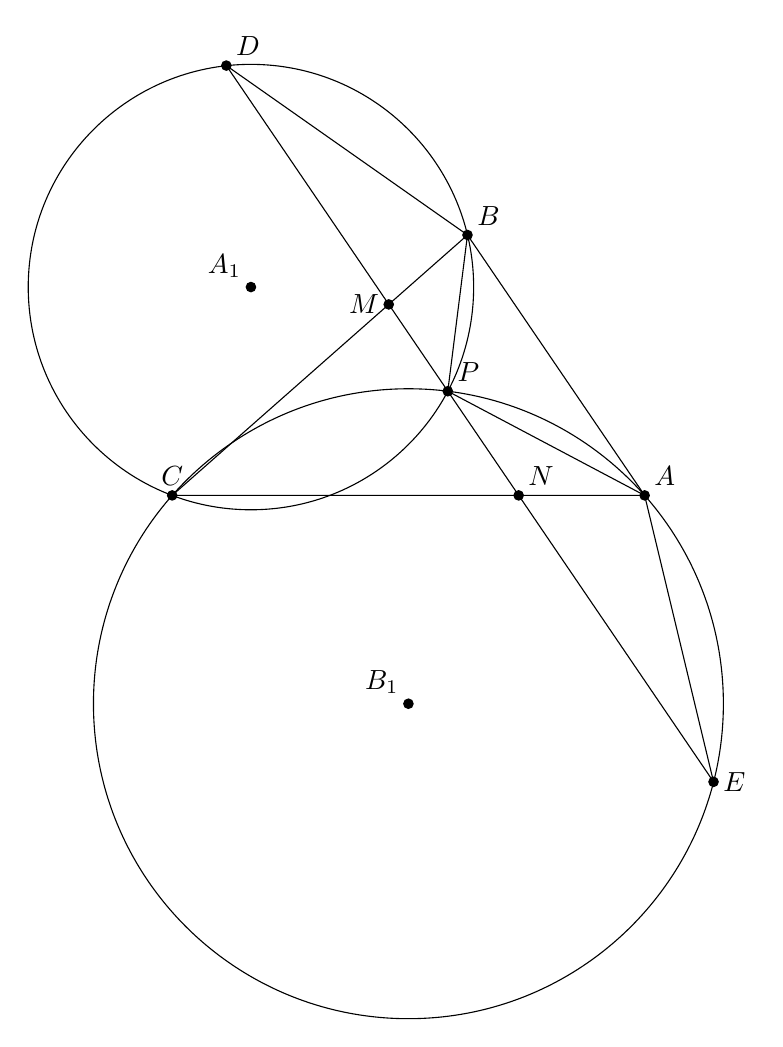
\begin{tikzpicture}
        \def\A{(6,0)}
        \def\B{(3.75,3.3071891)} 
        \def\C{(0,0)}
        \def\P{(3.5,1.3228756)} 
        \def\D{(0.6875,5.4586)} 
        \def\E{(6.875,-3.637908)} 
        \def\M{(2.75,2.42527203)}
        \def\N{(4.4,0)}
        \def\Aa{(1,2.64575)}
        \def\Bb{(3,-2.64575)}
        \filldraw \A circle (0.06) node[above right] {$A$};
        \filldraw \B circle (0.06) node[above right] {$B$}; 
        \filldraw \C circle (0.06) node[above] {$C$}; 
        \filldraw \P circle (0.06) node[above right] {$P$}; 
        \filldraw \D circle (0.06) node[above right] {$D$}; 
        \filldraw \E circle (0.06) node[right] {$E$}; 
        \filldraw \M circle (0.06) node[left] {$M$}; 
        \filldraw \N circle (0.06) node[above right] {$N$}; 
        \filldraw \Aa circle (0.06) node[above left] {$A_1$};
        \filldraw \Bb circle (0.06) node[above left] {$B_1$};
        \draw (3,-2.64575) circle (4);
        \draw (1,+2.645751) circle (2.82842);
        \draw \B -- \D -- \E -- \A -- \B -- \C -- \A -- \P -- \B;
        \end{tikzpicture}
    \end{figure}

    We claim $P$ is the incenter of $\triangle ABC$. By arc lengths, $\angle{PA'B} = 2 \angle BCP$ and since $A'P = A'B$ we have $\angle A'PB = 90 - \angle BCP \iff \angle APB = 90 + \angle BCP$.
    However, doing this to the circle centered at $B'$ gives $\angle APB = 90 + \angle ACP \iff \angle ACP = \angle BCP = \frac{\angle C}{2}$ and $\angle APB = 90 + \frac{\angle C}{2}$.
    The locus of all points such that $\angle APB = 90 + \frac{C}{2}$ is $(AIB)$, which the $C$-angle bisector intersects twice, once at $I$ and once outside of $\triangle ABC$; since $P$
    is specified to be inside $\triangle ABC$ we conclude $P \equiv I$. \medskip

    Since $\angle AEP = \angle ACP = \frac{\angle C}{2}$ and $\angle CAP = \angle APE = \frac{\angle A}{2}$ we have $\triangle{EAP} \cong \triangle CPA$ by AAS;
    similarly $\triangle CPB \cong \triangle DBP$ so $DE = EP + DP = AC + AB = 11$. Also, the tangents to the incircle from $A$ have length $s - a = \frac{5}{2}$
    and $[ABC] = rs \iff r = \frac{\sqrt7}{2}$ so $AP = 2 \sqrt 2$. \boxed{1210202}
\end{solution}\bigskip


        \newpage

        \subsubsection{``What's a signed integer?"}
            \label{8.2.6}
            \SSbreak\\
\emph{Source: \Cop}\\
\emph{Proposer: Constan\#6792}\\
\emph{Problem ID: 131}\\
\emph{Date: 2021-02-13}\\
\emph{Difficulty: Challenging}\\
\SSbreak

\SSpsetQ{
  For all pairs $ (n, q) $ where $ n $ is a positive integer, $ q $ is a rational non-integer, and $ n ^ q-q $ is an integer, find $\lfloor{n+q}\rfloor=x$. The sum of all possible values of $x$ is the answer. (For example, if we have $(1,1)$ and $(2,2)$, then the answer is $2+4=6$)
}\bigskip

\begin{solution}[Solution by Constan\#6792]\hfil\medskip
  
  Let's see that if $ n ^ q $ is rational and $ q $ is positive, $ n ^ q $ is integer.
To do this, suppose it is rational and not integer where $ (a, b) = (c, d) = 1 $.
$n^{\frac{a}{b}} = \frac{c}{d}$
$d^b . n^a = c^b$
Now we consider the exponent of a certain prime in the factorization of $ d, c, n $ which are $ e_d, e_c, e_n $ respectively.
$b. e_d + a .e_n = b. e_c$
$a.e_n \equiv 0 \; (b)$
$e_n \equiv 0 \; (b)$ 
So $ n $ is a $ b $ -th power.
$d^b . k^{ab} = c^b$
$d . k^a = c$
$k^a = \frac{c}{d}$
Absurd, because a perfect power must be a whole number.

Now if $ q $ is positive there are no solutions because if $ n ^ q $ and $ n ^ q-q $ are integers, $ q $ would be.

Then $n = -\frac{a}{b}$ with $ a $ and $ b $ co-prime positive integers and $ \frac {1} {n ^ {\frac {a}{b}}} + \frac {a}{b} $ is an integer.

Now if $\frac{n_1}{d_1} + \frac{n_2}{d_2} = \frac{n_1d_2+n_2d_1}{d_1d_2}$ is an integer where $(n_1, d_1) = (n_2, d_2) = 1$ we have to:
$d_1 | n_1d_2$ $\to$ $d_1|d_2$.
$d_2 | n_2d_1$ $\to$ $d_2|d_1$.
So $d_1 = d_2$.

That taking this to what we have tells us that $ n ^ {\frac {a} {b}} = b $ y
$ n ^ a = b ^ b $
Where with a very similar reasoning as before, $ b $ is a $ a $ -th power.
$b=k^a$
$n^a = k^{ak^a}$
$n=k^{k^a}$

$\frac{1}{(k^{k^a})^{\frac{a}{k^a}}} + \frac{a}{k^a} = \frac{a+1}{k^a}$

Where:
$ k ^ a \leq a + 1 $
If $ k \geq 3 $
$ 3 ^ a \leq k ^ a \leq a + 1$ has no solutions.
Then $ k \leq 2 $ where if $k=1$, $\frac{a}{b}$ would be an integer, so $ k = 2 $.
$ 2 ^ a \leq a + 1 $
Where the only solution is $a =1 $ that gives us the triple:
$(k^{k^a}, k^a, a) = (4, 2, 1)$.
Thus $ (n, q) = (4, - \frac {1} {2}) $ the only solution.
So the answer is $4$.
\end{solution}\bigskip

        \newpage

        \subsubsection{Diagonals in a Convex 1001-gon}
            \label{8.2.7}  
            \SSbreak\\
\emph{Source: Sharygin 2019 Finals Grade 8 P8}\\
\emph{Proposer: \Pnjoy}\\
\emph{Problem ID: 132}\\
\emph{Date: 2021-02-14}\\
\emph{Difficulty: Challenging}\\
\SSbreak

\SSpsetQ{
  What is the least positive integer \(k\) such that, in every convex 1001-gon, the sum of any \(k\) diagonals is greater than or equal to the sum of the remaining diagonals?
}\bigskip

\begin{solution}\hfil\medskip
  \href{https://geometry.ru/olimp/2019/final_sol_eng.pdf}{Offical Solution, page 6 P8}

  Answer: \fbox{499000}
\end{solution}\bigskip

        \newpage

\setcounter{section}{9}
\ihead{\footnotesize\bfseries\sffamily{CCCC After Math (Season 10)}}
\section{CCCC After Math (Season 10)}

    \ihead{\footnotesize\bfseries\sffamily{CCCC After Math (Season 10), Week 1}}
    \subsection{Week 1}

        \subsubsection{Epic\textcolor{red}{X}troll}
        \label{10.1.1}
        \SSbreak\\
\emph{Source: Original}\\
\emph{Proposer: \Ptroll}\\ %\Pchan \Pbrain \Pss
\emph{Problem ID: 133}\\
\emph{Date: 2021-02-15}\\
\emph{Difficulty: Beginner}\\
\SSbreak

\SSpsetQ{
	How many possibilities are there for the total score among all participants at the end of a standard QoTD season? (Assume that no rounding occurs. Recall that a standard QoTD season has $14$ questions.)
	%Put Problem Here
}\bigskip

\begin{solution}\hfil\medskip
	
    The answer is $\boxed{15}$: if $0 \le N \le 14$ is the number of questions solved (by anyone), then the total score is $1000N$.
	%Put sol here
\end{solution}\bigskip

        \newpage

        \subsubsection{Similar Triangles}
        \label{10.1.2}  
        \SSbreak\\
\emph{Source: Original}\\
\emph{Proposer: \Pmatt}\\ %\Pchan \Pbrain \Pss
\emph{Problem ID: 134}\\
\emph{Date: 2021-02-16}\\
\emph{Difficulty: Beginner}\\
\SSbreak

\SSpsetQ{
	Let $ABC$ be a triangle with $AB = AC$ and $BC = 10$. Construct $D$ and $E$ outside $ABC$ closer to $B$ and $C$ respectively such that $\triangle DAB \sim \triangle ABC \sim \triangle EAC$. \medskip
	
	If $DE = 45$, then what is $AB$?
	%Put Problem Here
}\bigskip

\begin{solution}\hfil\medskip

	\begin{figure}[h!]
			\centering
		\begin{tikzpicture}[scale = 0.01cm]
		\def\B{(-5,0)}
		\def\C{(5,0)}
		\def\A{(0,14.1421356)}
		\def\D{(-22.5,14.1421356)}
		\def\E{(22.5,14.1421356)}
		\draw \B -- \A -- \C -- \B -- \D -- \E -- \C;
		\filldraw \A circle (0.15) node[above] {$A$};
		\filldraw \B circle (0.15) node[below left] {$B$};
		\filldraw \C circle (0.15) node[below right] {$C$};
		\filldraw \D circle (0.15) node[left] {$D$};
		\filldraw \E circle (0.15) node[right] {$E$};
		\end{tikzpicture}
	\end{figure}


	Note that $\angle DAB = \angle ACB = \angle ABC$ and hence $AD \parallel BC$. Similarly $AE \parallel BC$ and so $A$ is the midpoint of $DE$, and $A, D, E$ are collinear. \medskip
	
	So $AD = 22.5$ and hence $AB = BC * \sqrt{\frac{AD}{BC}}$ by similarity, which is $\boxed{15}$. 
	%Put sol here
\end{solution}\bigskip

        \newpage

        \subsubsection{Factorial Sums and Divisors}
        \label{10.1.3}  
        \SSbreak\\
\emph{Source: \Cfolk}\\
\emph{Proposer: \Pss}\\
\emph{Problem ID: 135}\\
\emph{Date: 2021-02-17}\\
\emph{Difficulty: Easy}\\
\SSbreak
 
\SSpsetQ{
   What is the largest prime number which divides

   \[0!+1!\times1+2!\times2+3!\times3+\cdots+159!\times 159 + 160!\times 160\]
}\bigskip

\begin{solution}\hfil\medskip

We proceed by using the identity \(n!+n!\times n = (n+1)!\) and iterating:
\begin{align}
    &0!+1!\times 1+\cdots\\
    &2!+2!\times2+\cdots\\
    &3!+3!\times3+\cdots\\
    &\cdots\\
    &161!
\end{align}
As neither 161 nor 159 are prime, the largest prime divisor of the sum is \fbox{157}
\end{solution}\bigskip

\begin{solution}\hfil\medskip

    Note that $(n + 1)! - 1$ counts the non-identity permutations of $(1, 2, \cdots , n + 1)$. 
    Consider a permutation where $(1, 2, \cdots n - k)$ are fixed points but $n - k + 1$ is not a fixed point.
    So $n - k + 1$ can go in the $n - k + 2^{\text{nd}}$ to $n + 1^{\text{st}}$ spots, which is a total of $k$ possibilites;
    the remainder of the $k$ terms can be permuted willy-nilly. Thus, there $k \cdot k!$ such possibilities, and summing over 
    $k$ from $1$ to $n$ (since $k = n + 1$ gives the identity permutation) yields the identity. \fbox{157}
\end{solution}
        \newpage

        \subsubsection{Brainy's Passcode}
        \label{10.1.4}  
        \SSbreak\\
\emph{Source: Italian team competition}\\
\emph{Proposer: \Phobo}\\ %\Pchan \Pbrain \Pss
\emph{Problem ID:}\\
\emph{Date: }\\
\emph{Difficulty: Medium}\\
\SSbreak

\SSpsetQ{
	Brainy forgot the numerical unlock code of his Nokia once again... This time he remembers that it is 69-digits long and the leading digit is greater or equal than the sum of all the remaining digits. Find the total number of possible codes.  \medskip
	
	\begin{center}
		\emph{A computational aid may be used to calculate the final answer.}
	\end{center}
	%Put Problem Here
}\bigskip

\begin{solution}\hfil\medskip

Let $n$ be the number of digits of the code, in our case $n=69$ and let $k$ be the leading digit, clearly $k\in\{1,2,\dots,9\}$. Let $i$ be the sum of the remaining digits, where $i\in\{1,2,\dots,k\}$. Using the stars and bars method (also called sticks and stones or Tonys and Wangs), the number of possible codes (with $k$ and $i$ fixed) is $$\binom{(n-1)-1+i}{(n-1)-1}$$ Cycling this for all possible values of $k$ and $i$ we get the following expression $$\sum_{k=1}^{9}\sum_{i=0}^{k}\binom{n-2+i}{n-2}$$ Using the Hockey-stick identity 2 times in a row we get 
\begin{align*}
    \sum_{k=1}^{9}\sum_{i=0}^{k}\binom{n-2+i}{n-2}&=\sum_{k=1}^{9}\binom{k+n-1}{k} \\
    &=\binom{n+9}{9}-1
\end{align*}

Plugging in $n = 69$ we get $$\binom{78}{9} - 1 = \boxed{182364632449}.$$
	
	%Put sol here
\end{solution}\bigskip

\begin{solution}[Write up by \Paiya]\hfil\medskip

	Let the $k^\text{th}$ digit from the left be $d_k$. Our constraints become $9 \leq d_1 \leq \sum_{k = 2}^{69} d_k$; let $y = 9 - d_1$ and $x = d_1 - \sum_{k = 2}^{69}d_k$.
	Our contraints become $$9 = d_1 + y = x + y + \sum_{k = 2}^{69} d_k$$ so it suffices to count the ways to distribute 9 objects among 70 people.
	Letting 69 "sticks" divide the 9 "stones" into 70 parts, we see that this is $\binom{78}{9}$ then subtract 1 because a string of 69 zeros is invalid. \fbox{182364632449}
\end{solution}
        \newpage

        \subsubsection{Production Loop}
        \label{10.1.5}  
        \SSbreak\\
\emph{Source: Original/Folklore}\\
\emph{Proposer: \Paiya}\\ %\Pchan \Pbrain \Pss
\emph{Problem ID:}\\
\emph{Date: }\\
\emph{Difficulty: Hard (CN4)}\\
\SSbreak

\SSpsetQ{
    Let $f: \mathbb{N} \to \mathbb{N}$ be a function defined as follows: $$f(n) = 2n + 1 - 2^{\lfloor \log_2n \rfloor + 1}$$ 
    and let $f^a(n) = f\left(f^{a - 1}(n)\right)$. Let $t(n)$ be the smallest positive integer such that 
    there exists a positive integer $N$ such that $f^{t(n)}(n) = f^{t(n) + N}(n)$. 
    Determine the remainder when $\sum_{n = 2^{2020}}^{2^{2021}} f^{t(n)}(n)$ is divided by $1009$. \medskip
    
    \textit{(A scientific calculator can be used)}
	%Put Problem Here
}\bigskip

\begin{solution}\hfil\medskip
	
    Consider what $f$ does to $n$ in binary: $2n + 1$ concatenates a $1$ to the end of $n$, while 
    $2^{\lfloor \log_2n \rfloor + 1}$ subtracts the concatenation of $0$ to the end of $n$ from $2n + 1$. 
    This can be seen as cycling the leading $1$ of $n$ to the end of $n$; for instance $f\left(6 = 101_2\right) = 11_2 = 3$. 
    After applying $f$ enough times, we're left with the number of ones present in $n$. We now count the number of integers $2^{2020} \leq n < 2^{2021}$
    which have $k$ ones present in their binary representation. All these numbers are 2021 digits long, so we want to distribute $k - 1$ ones among $2020$ digits;
    there are $\binom{2020}{k - 1}$ ways to do this and each such $n$ contributes $2^k - 1$ to the sum. 
    Remembering that $f^{t(n)}(n) = 1$ when $n = 2^{2021}$, it remains to sum 
    \begin{align*}
        1 + \sum_{k = 1}^{2021} \dbinom{2020}{k - 1}\left(2^k - 1\right) &= 1 + 2\sum_{k = 1}^{2021} \dbinom{2020}{k - 1}2^{k - 1} - \sum_{k = 1}^{2021} \dbinom{2020}{k - 1} \\
        &= 1 + 2 \cdot 3^{2020} - 2^{2020} \\
        &\equiv 1 + 2 \cdot 81 - 16 \pmod{1009}\\
        &= \boxed{147}
    \end{align*}
    where we have used $(1 + 2)^n = \sum_{k = 0}^n \binom{n}{k} 2^k = 3^k$ to help simplify.
	%Put sol here
\end{solution}\bigskip

        \newpage

        \subsubsection{Weird polynomial}
        \label{10.1.6}  
        \SSbreak\\
\emph{Source: NYCMT, 2020 P9 of 10}\\
\emph{Proposer: \Pnjoy}\\
\emph{Problem ID: }\\
\emph{Date: }\\
\SSbreak

\SSpsetQ{
Let \( p = 2053 \) be a prime. For positive integers \( x\) let 
\[ f(x) = x^{400} + x^{326} + x^{200} + x^{126} + 2\]
and let \( g(x)\) denote the unique integer \(0\leq y \leq p-1\) such that \( y^{1759} - x \) is divisible by \( p\). Compute the remainder when 
\[ \sum_{i=1}^{2052} g(f(i)) \] 
is divided by 2053. 
}\bigskip

\begin{solution}\hfil\medskip

    To find $y$, we want to raise $y^{1759} \equiv x \pmod{p}$ to a power $k$ such that $1759k \equiv 1 \pmod{p - 1}$; solving we get $k \equiv 7 \pmod{p - 1}$
    and so $y \equiv x^7 \pmod{p}$. It remains to sum $f(i)^7 \pmod{p}$. Since $g, g^2, \cdots , g^{p - 1}$ where $g$ is a generator is a permutation of the nonzero residues mod $p$
    we find that $$\sum_{i = 1}^{p - 1} i^k = \sum_{i = 1}^{p - 1} g^{ik} = g^k \left(\dfrac{g^{(p - 1)k} - 1}{g^k - 1}\right) \equiv 0 \pmod{p}$$ unless $p - 1 | k$
    in which case each of the $p - 1$ terms is $1$ for a sum of $-1 \pmod{p}$. Since the maximum coefficient in $f(x)^7$ is $7 \cdot 400 = 2800$ it suffices to
    find the coefficient of $x^{2052}$ and the constant term. Using multinomial expansion, this is equivalent to finding nonnegative integers $(a, b, c, d, e)$ 
    such that $400a + 326b + 200c + 126d + 0e = 2052 \iff 200a + 163b + 100c + 63d = 1026$ and $a + b + c + d + e = 7$. Notice $a > 1$ since $200 \cdot 1 + 163 \cdot 6 < 1026$ and 
    $a < 5$ since $200 \cdot 5 = 1000$ and no combination of $160, 100, 63$ will make that sum to $1026$. Also, reducing mod 9 yields $2a + b + c \equiv 0 \pmod{9} \iff a + 7 \equiv d + e \pmod{9}.$
    When $a = 2$, we are forced $d, e = 0$ so $163b + 100c = 626 \iff (a, b, c, d, e) = (2, 2, 3, 0, 0)$.
    When $a = 3$, we are forced $d = 0, 1$ so either $163b + 100c = 426, 363 \iff (a, b, c, d, e) = (3, 2, 1, 0, 1), (3, 1, 2, 1, 0)$.
    When $a = 4$, we have $163b + 100c + 63d = 226 \iff (a, b, c, d, e) = (4, 1, 0, 1, 1), (4, 0, 1, 2, 0)$.
    Remembering the constant term is $2^7$, it remains to sum 
    $$-\dbinom{7}{2, 2, 3, 0, 0} - 2\dbinom{7}{3, 2, 1, 0, 1} - \dbinom{7}{3, 1, 2, 1, 0} - 2\dbinom{7}{4, 1, 0, 1, 1} - \dbinom{7}{4, 0, 1, 2, 0} - 2^7 \equiv \boxed{1983} \pmod{2053}.$$
\end{solution}\bigskip

        \newpage
		
		\subsubsection{Weird triangle}
		\label{10.1.7}
		\SSbreak\\
\emph{Source: Original}\\
\emph{Proposer: \Ptan}\\ %\Pchan \Pbrain \Pss
\emph{Problem ID: 139}\\
\emph{Date: 2021-02-21}\\
\emph{Difficulty: Challenging (G7)}\\
\SSbreak

\SSpsetQ{
	Let $ABC$ be a $13-14-15$ triangle, with $AC = 14$. Points $X, Y$ satisfy \[CX - BX = BX - AX = 1 = AY - BY = BY - CY.\]
	
	The value of $XY$ can be written in the form $\frac{a \sqrt{b}}{c}$, where $b$ is not divisible by the square of any prime and $a$ and $c$ are relatively prime positive integers.
	Find $10000a + 100b + c$.  
	%Put Problem Here
}\bigskip

\begin{solution}\hfil\medskip

	Let $I$ be the incenter of $\triangle ABC$. Construct three circles, each centered at one of $A$, $B$, $C$. Note that these three circles touch each other at the three intouch points of $\triangle ABC$. Thus their radii are 6, 7 and 8. WLOG assume AB = 13. Let $W$ be the center of the unique circle externally tangent to our three circles at $A$, $B$, $C$, and $Z$ the center of the unique circle internally tangent to our three circles at $A$, $B$, $C$. By definition, since the radius of the circle at $C$ is 8, the radius of the circle at $B$ is 7 and the radius of the circle at $A$ is 6, $W$ and $Z$ must be precisely $X$ and $Y$. Now consider an inversion with respect to the incircle. Let the intersection of the line $AI$ and the circle at $A$ further from $I$ be $D$, and the one closer to $I$ be $E$. Then if the radius of the circle at $A$ is $R$, and the inradius is $r$, $DI \cdot EI = (AI - R)(AI + R) = AI^2 - R^2 = R^2 + r^2 - R^2 = r^2$, so by definition $D$ and $E$ swap under our inversion. Thus the circle at (A) must map to itself under our inversion, and so do the circles at (B) and (C). Then since inversion preserves tangency, the circle at $X$ externally tangent to our three circles must swap with the circle at $Y$ internally tangent to our three circles. \medskip

	Now suppose a line through $I$ meets the circle at $X$ at $M$, $N$ and the circle at $Y$ at $P$, $Q$. Then since the image of $M$ must lie on the ray $MI$, and also lie on the circle at $Y$ since $M$ lies on the circle at $X$, WLOG $M$ and $P$ swap, and then so do $N$ and $Q$. Thus $IM \cdot IP = r^2 = IN \cdot IQ$, and by power of a point $IM \cdot IN = {R_x}^2 - IX^2$ and $IN \cdot IQ = {R_y}^2 - IY^2$ where $R_x$ and $R_y$ are the radii of the circles at $X$ and $Y$. Since $IM \cdot IP$ is independent of $M$ and $P$ we find that $I$ is the insimilicenter of the circles at $X$ and $Y$ and therefore lies on the line segment $XY$.
	Thus if we set $IX = cR_x$ and $IY = cR_y$ then $r^4 = {R_x}^2{R_y}^2(1 - c^2)^2$; by direct calculation (the inradius formula for $r$ and Descartes' Kissing Circles Theorem for $R_x$ and $R_y$) we obtain four values for $c$.
	However, two of these values are negative and a third is greater than 1 (we know that clearly $IX$ and $IY$ are smaller than $R_x$ and $R_y$ by simply drawing the diagram in this case), so the only acceptable value of $c$ is $c = \frac{\sqrt{37}}{42}$. Then by direct calculation we obtain that $XY = IX + IY = cR_x + cR_y = \frac{672\sqrt{37}}{1727}$ so the answer is $\boxed{6725427}$ as required.
\end{solution}\newpage

\begin{solution}\hfil\medskip
	
	An elementary, computationally feasible analytic solution is still possible using Cartesian coordinates. From the given condition, if we let $BX = d$ then $AX = d - 1, CX = d + 1$. 
	Consider circles $\omega_A, \omega_B, \omega_C$ centered at $A, B, C$ with radii $d - 1, d, d + 1$ respectively. 
	Let $A = (-5, 0), B = (0, 12), C = (9, 0)$. Then the radical axis of $\omega_A$ and $\omega_C$ is given by
	$$(x + 5)^2 + y^2 - (d - 1)^2 = (x - 9)^2 + y^2 - (d + 1)^2 \iff 7x = 14 - d$$
	and the radical axis of $\omega_A$ and $\omega_B$ is given by
	$$(x + 5)^2 + y^2 - (d - 1)^2 = x^2 + (y - 12)^2 - d^2 \iff 5x + 12y = 60 - d$$
	so the radical center of $\omega_A, \omega_B, \omega_C$ satisfies $$(x, y) = \left(\dfrac{14 - d}{7}, \dfrac{350 - 2d}{84}\right).$$
	This point must be on $\omega_B$, so plugging in and simplifying we have
	$$\left(\dfrac{14 - d}{7}\right)^2 + \left(\dfrac{350 - 2d}{84} - 12\right)^2 = d^2 \iff \dfrac{1727}{1764}d^2 + \dfrac{25}{126}d - \dfrac{2353}{36} = 0.$$
	Solving this quadratic would be hell, but we don't need to. Let the two roots be $r, s$ with $r$ positive and $s$ negative. Consider a point $P$ with
	$PA = |s - 1|, PB = |s|, PC = |s + 1|$; since $s < -1$ we have $PA = -s + 1, PB = -s, PC = -s - 1$. This satisfies $AP - BP = BP - CP = 1$, so $P \equiv Y$! Thus, it remains to find
	$$XY = \sqrt{\dfrac{(r - s)^2}{7^2} + \dfrac{(r - s)^2}{42^2}} = \dfrac{r - s}{7} \sqrt{\dfrac{37}{36}}$$
	and now the miraculous 
	$$(r - s)^2 = (r + s)^2 - 4rs = \dfrac{1764^2}{1727^2} \left(\dfrac{25^2}{126^2} + \dfrac{2353}{9} \cdot \dfrac{1727}{1764}\right) = 256 \cdot \dfrac{1764^2}{1727^2} \iff r - s = 16 \cdot \dfrac{1764}{1727}$$
	so $XY = \frac{672 \sqrt{37}}{1727} \iff \boxed{6725427}.$
	
	%Put sol here
\end{solution}\bigskip

		\newpage

    \ihead{\footnotesize\bfseries\sffamily{CCCC After Math (Season 10), Week 2}}
    \subsection{Week 2}

        \subsubsection{Real Square Roots}
        \label{10.2.1}  
        \SSbreak\\
\emph{Source: Purple Comet! Math Meet, High School, 2020 P4}\\
\emph{Proposer: \Pnjoy}\\ %\Pchan \Pbrain \Pss
\emph{Problem ID: 140}\\
\emph{Date: 2021-02-22}\\
\emph{Difficulty: Beginner}\\
\SSbreak

\SSpsetQ{
	Let $\mathcal{S}$ be the set of integers $n$ such that $$\sqrt{\frac{(2021-k)^2}{2021-k^2}}$$ is a real number. \medskip
	
	Compute the sum of all elements in $\mathcal{S}$. 
	%Put Problem Here
}\bigskip

\begin{solution}\hfil\medskip
	
	The numerator is always real, so we seek $k$ such that $2021 - k^2 > 0$; however if $k$ satisfies this inequality so does $-k$. Then observe
	$k = 2021$ makes the numerator 0, so it is real too. $\boxed{2021}$.
	%Put sol here
\end{solution}\bigskip

        \newpage

        \subsubsection{"What's a positive integer?"}
        \label{10.2.2}  
        
\SSbreak\\
\emph{Source: \Cop}\\
\emph{Proposer: \Pnjoy}\\
\emph{Problem ID: 141}\\
\emph{Date: 2021-02-23}\\
\emph{Difficulty: Beginner}\\
\SSbreak

\SSpsetQ{
  Let $n$ be a positive integer. Find the number of positive divisors of $69420^{69}$ which are of the form $4n+1$.
}\bigskip

\begin{solution}[Solution by \Pnjoy]\hfil\medskip

  Note that $69420^{69}=2^{138}\cdot 3^{69}\cdot 5^{69}\cdot 13^{69}\cdot 89^{69}$. From these, only $3$ is a prime which is equivalent to $3 \pmod{4}$ and others, i.e. $5, 13, 89$ are all $1\pmod{4}$. Therefore, the number of ways to choose a divisor of the form $4n+1$ is $35 \times 70\times 70\times 70$\footnote{$35$ ways being for the even powers of $3$ and $70$ otherwise}. But, since $n$ is positive integer, so $1$ can not be a chosen divisor. Hence, the desired answer is $35\cdot 70^3 - 1 = \boxed{12004999}$.
\end{solution}\bigskip

        \newpage
			
        \subsubsection{Converging Tangent Circles}
        \label{10.2.3}  
        \SSbreak\\
\emph{Source: \Cop}\\
\emph{Proposer: \Phobo}\\ %\Pchan \Pbrain \Pss
\emph{Problem ID: 142}\\
\emph{Date: 2021-02-24}\\
\emph{Difficulty: Easy}\\
\SSbreak

\SSpsetQ{
	In the following diagram every circle has two internally tangent circles also tangent to each other. The radius of the biggest circle is $\frac{1}{\sqrt{\pi}}$. If the area of the black region can be expressed as $\frac{a}{b}$, compute $100a+b$.
	%Put Problem Here
}\bigskip

\begin{figure}[ht]
	\centering
	
\begin{tikzpicture}
		\foreach \x in {0}  \draw[fill,color = black] (\x,0) circle (2cm);
		\foreach \x in {0,...,1}  \draw[fill,color = white] (-1+2*\x,0) circle (1cm);
		\foreach \x in {0,...,3}  \draw[fill,color = black] (-1.5+1*\x,0) circle (0.5cm);
		\foreach \x in {0,...,7}  \draw[fill,color = white] (-1.75+0.5*\x,0) circle (0.25cm);
		\foreach \x in {0,...,15} \draw[fill,color = black] (-1.875+0.25*\x,0) circle (0.125cm);
		\foreach \x in {0,...,31} \draw[fill,color = white] (-1.9375+0.125*\x,0) circle (0.0625cm);
		\foreach \x in {0,...,63} \draw[fill,color = black] (-1.96875+0.0625*\x,0) circle (0.03125cm);
	\end{tikzpicture}
\end{figure}

\begin{solution}[Solution by \Phobo]\hfil\medskip
	
	Let $r_n$ and $A_n$ be the radius and the area of the nth circle (in descending order). From construction we have $r_{n+1}=\frac{r_{n}}{2}$ which leads to $r_n=\frac{r_0}{2^n}$, where $r_0=\frac{1}{\sqrt{\pi}}$. Looking at the desired area $A_{\zeta}$ as difference of black and white circles areas, we get the following:
	\begin{align}
		A_{\zeta}&= \sum_{n=0}^{\infty}(-2)^n A_{n} \\
		&=\sum_{n=0}^{\infty}(-2)^n (r_n)^2 \pi \\
		&=(r_0)^2 \pi \sum_{n=0}^{\infty}\left(-\frac{1}{2}\right)^n \\
		&=\left(\frac{1}{\sqrt{\pi}}\right)^2\pi\frac{1}{1-\left(-\frac{1}{2}\right)} \\ 
		&= \frac{2}{3}
	\end{align}
	Which means $\boxed{203}$ is the solution.
\end{solution}\bigskip

\begin{solution}[Solution by \Pflame]\hfil\medskip

	Let $B$ be the total black area; the total white area is then $1 - B$. Looking at the two biggest white circles, we see that each of them is similar
	to the big circle by a factor of $\frac{1}{2}$ with colors inverted; thus the total black area inside each of the two white circles is $\frac{1 - B}{4}$.
	Since the black area outside the two big white circles is $\frac{1}{2}$ we have $$B = \dfrac{1}{2} + \dfrac{1 - B}{2} \iff B = \dfrac{2}{3} \iff \boxed{203}.$$
\end{solution}
        \newpage

        \subsubsection{Maze Escape}
        \label{10.2.4}
        \SSbreak\\
\emph{Source: 2018 HMMTNov Guts 18}\\
\emph{Proposer: \Paiya}\\ %\Pchan \Pbrain \Pss
\emph{Problem ID: 143}\\
\emph{Date: 2021-02-25}\\
\emph{Difficulty: Medium (C3)}\\
\SSbreak

\SSpsetQ{
    MODSbot has trapped Brainy at the southwest entrance of a two-by-fifteen grid of cells. To escape, Brainy has to enter into the grid from the southwest cell
    and exit through the northeast cell. However, MODSbot can fill any subset of the 20 cells with cement, effectively blocking off those cells.
    Out of all $2^{30}$ possible grid configuations, in how many of them can Brainy escape?
	%Put Problem Here
}\bigskip

\begin{solution}\hfil\medskip
	
    Follow the \href{https://hmmt-archive.s3.amazonaws.com/tournaments/2018/nov/guts/solutions.pdf}{official solution} to get the recursion for $a_n$ and $b_n$.
    Iterating 15 indices of $a$ and $b$ is inefficient; for efficient computation we let $c_n = a_n + b_n$ and note that $c_{n + 1} = 2c_n + c_{n - 1}$; either directly recursing or finding a closed form yields 
    $c_{15} = 665857$. By inspection, we have $a_n = b_n - 1$ so $a_n = \boxed{332928}$.
	%Put sol here
\end{solution}\bigskip
        \newpage 

        \subsubsection{Primes divide powers of 5}
        \label{10.2.5}  
        \SSbreak\\
\emph{Source: China National Olympiad 2009, P2}\\
\emph{Proposer: \Pmatt}\\ %\Pchan \Pbrain \Pss
\emph{Problem ID:}\\
\emph{Date: }\\
\emph{Difficulty: Hard}\\
\SSbreak

\SSpsetQ{
	Suppose \(\mathcal{S}\) is the set of all pairs \((p, q), p \leq q\) such that \[pq \mid 5^p + 5^q.\] \medskip
	
	Find \[\sum_{(p, q) \in \mathcal{S}} (1000p + q).\]
	%Put Problem Here
}\bigskip

\begin{solution}\hfil\medskip
	
	\href{https://artofproblemsolving.com/community/c6h250256p1371288}{AoPS Solution} \medskip
	
	Answer: \(\boxed{14326}\)
	%Put sol here
\end{solution}\bigskip

        \newpage

        \subsubsection{tRiViaL}
        \label{10.2.6}  
        
\SSbreak\\
\emph{Source: \Cop}\\
\emph{Proposer: QuantumSigma\#9996}\\
\emph{Problem ID: }\\
\emph{Date: }\\
\emph{Difficulty: Challenging}\\
\SSbreak

\SSpsetQ{
  Consider an integer-valued function $f(x, y)$ defined on the lattice points of the $x-y$-plane. The value of $f$ at each point is average its 4 neighbours. The difference in $f$ is less than 70000 for any pair of lattice points a distance of exactly 2021 apart. If $f(a, b + c) - f(a, b) = 1780$ for some integers $(a, b, c)$, find the sum of all possible $\abs{c}$.
}\bigskip

\begin{solution}[Solution by QuantumSigma\#9996]\hfil\medskip
    $3738.$
Let $F$ be the set of functions $g: Z^2 \rightarrow Z$ fulfilling the 'average of neighbours' criteria.
\begin{enumerate}
    \item For any $g \in F$, $g$ is either constant or unbounded (Klarijōn\#0829, modified). Proof: Assume there exist 2 adjacent points $(A, B)$ such that $g(A) < g(B)$. Then there exists point $C$ adjacent to $B$ such that $g(B) < g(C)$. Repeating ad infinitum, there exists an infinite strictly monotonic chain of points. Thus $g$ is unbounded.
    \item Define $P$ and $Q$:
    \begin{align*}
        P{f}(x, y) &= f(x + 2021, y) - f(x, y)\\
        Q{f}(x, y) &= f(x, y + 2021) - f(x, y)
    \end{align*}
    Then for any $g \in F, P\{g\}, Q\{g\} \in F$ (trivial)
    \item For any $f \in F$ such that $P\{f\}, Q\{f\}$ are bounded, $f$ is linear. Proof: By $(1)$ and $(2)$, $P{f}, Q{f}$ are constant. Let $h = 2021f - P{f}x - Q{f}y$, then $h \in F$. Since $h$ is doubly periodic (trivial), it is bounded, and thus constant. Then $f = \frac{P{f}x + Q{f}y + h}{2021}$.
\end{enumerate}
It follows that $\abs{c}$ is a factor of 1780.
The problem is then trivial.
\end{solution}\bigskip

        \newpage

        \subsubsection{Lamps in a Circle}
        \label{10.2.7}  
          
\SSbreak\\
\emph{Source: Olympic Revenge, 2013 P5}\\
\emph{Proposer: \Pchris}\\ %\Pchan \Pbrain \Pss
\emph{Problem ID:}\\
\emph{Date: }\\
\SSbreak

\SSpsetQ{
    Suppose \(n\) lamps are arranged in a circle, numbered from 1 to \(n\) clockwise, with \(0\geq L \geq n\) lamps turned on. A testing procedure consists of performing the following operations: 
    \begin{itemize}
        \item for each lamp turned on, we take its number \(i\); the \(i\) lamps following it clockwise receive a signal
        \item After a signal has been sent for each lamp turned on, every lamp which received an odd number of signals will have its state changed; those receiving an even number of signals will not.
    \end{itemize}
       Let \(T\) be the set of all \(2^n\) possible initial configurations. We define a function \(t\) from \(T\) to \(T\), where if \(X\) represents an initial configuration of lamps, \(t(X)\) is the configuration obtained after applying the testing procedure to \(X\). Suppose \(S\) is the sum of all integers \(n < 2^{2015}\) such that the function \(t\) is bijective. Find the smallest positive integer \(c\) such that \(2^c\) is greater than the sum of every element of \(S\). 

}\bigskip

\begin{solution}\hfil\medskip
    \href{ https://artofproblemsolving.com/community/c6h518190p2916501}{(Art of Problem Solving write ups)}
\end{solution}\bigskip

        \newpage

\ihead{\footnotesize\bfseries\sffamily{err¶¶: ¶¶ ¶¶¶ ¶¶¶¶¶¶¶ ¶¶¶¶ ¶¶ ¶¶¶ ¶¶¶¶ ¶¶¶¶¶. (Season 11)}}
\section{err¶¶: ¶¶ ¶¶¶ ¶¶¶¶¶¶¶ ¶¶¶¶ ¶¶ ¶¶¶ ¶¶¶¶ ¶¶¶¶¶. (Season 11)}

    \ihead{\footnotesize\bfseries\sffamily{err¶¶: ¶¶ ¶¶¶ ¶¶¶¶¶¶¶ ¶¶¶¶ ¶¶ ¶¶¶ ¶¶¶¶ ¶¶¶¶¶. (Season 11), Week 1}}
    \subsection{Week 1}

        \subsubsection{Integral AM-GM}
        \label{11.1.1}
        \SSbreak\\
\emph{Source: Original}\\
\emph{Proposer: \Ptan\, and \Pwen}\\
\emph{Problem ID:}\\
\emph{Date: }\\
\emph{Difficulty: Beginner}\\
\SSbreak

\SSpsetQ{
  $p, q$ are positive integers such that $pq = 2021^{2021}.$ What is the minimal number of digits in $p + q?$
}\bigskip

\begin{solution}\hfil\medskip
  
By AM-GM the minimal value of $p + q$ occurs when $p, q$ are close; an obvious close pair is $(p, q) = \left(43^{1010}, 47^{1010}\right)$
and the minimal possible value of $p + q$ (over positive reals) occurs at $p = q = 2021^{1010.5}$. The number of digits in a number $n$
is $\left\lfloor \log_{10}(n) \right\rfloor + 1$; noticing this we see that both our obvious guess and the absolute minimum have \fbox{3341} digits.
\end{solution}\bigskip

        \newpage

        \subsubsection{d20 but not D20}
        \label{11.1.2}
        \SSbreak\\
\emph{Source: Original}\\
\emph{Proposer: \Ptan\, and \Pwen}\\
\emph{Problem ID: 148}\\
\emph{Date: 2021-03-02}\\
\emph{Difficulty: Beginner}\\
\SSbreak

\SSpsetQ{
    $21$ people, including IcosahedralDice, each roll an icosahedral die, which have faces numbered $1$ through $20$ and each face is equally likely to land face-up. Given that IcosahedralDice rolled the (strictly) largest number, find the expected value of his roll.
}\bigskip

\begin{solution}\hfil\medskip
  
    Let IcosahedralDice roll $r$. The probability that a person rolls between $1$ and $r - 1$ inclusive is $\frac{r - 1}{20}$ so the probability that all $20$
    other people rolled less than $r$ is $\left(\frac{r - 1}{20}\right)^{20}$; thus the probability IcosahedralDice's roll is strictly greater than everyone else's
    is $\sum_{r = 1}^{20} \left(\frac{r - 1}{20}\right)^{20}$. The expected value is then
    $$E = \dfrac{\sum_{r = 1}^{20} r \cdot \left(\frac{r - 1}{20}\right)^{20}}{\sum_{r = 1}^{20} \left(\frac{r - 1}{20}\right)^{20}} \iff \left\lfloor 100000E \right\rfloor = \boxed{1952901}.$$
\end{solution}\bigskip

        \newpage

        \subsubsection{Is it better to walk or run in the rain?}
        \label{11.1.3}
        \SSbreak\\
\emph{Source: Original}\\
\emph{Proposer: \Ptan\, and \Pwen}\\
\emph{Problem ID:}\\
\emph{Date: }\\
\emph{Difficulty: Easy}\\
\SSbreak

\SSpsetQ{
    Rain is falling at an angle of 2.021 (radians) measured anticlockwise from the positive $x$-axis, with velocity 2021. A unit sphere rolls from the origin to $(2021, 0)$
    with constant speed $v$. \medskip
    
    Given that $v$ minimizes the amount of rain that falls on the ball, find $\lfloor 10^2v \rfloor$, where $\lfloor x \rfloor$ is the greatest integer less than or equal tos $x$. \medskip
    
    \begin{center}
    	\emph{Note that if you run too fast, you end up running \emph{into} the rain.}
    \end{center}
}\bigskip

\begin{solution}\hfil\medskip
  
    Change the frame of reference such that the rain is still relative to you; this can be done by moving the entire plane with velocity $(2021 \cos \theta, 2021 \sin \theta)$
    where $\theta = 2.021$, the angle at which rain falls. This means that your destination point will be on the line with slope $\tan \theta$ passing through $(2021, 0$
    and your new velocity vector is $(v + 2021 \cos \theta, 2021 \sin \theta)$. To minimize the amount of rain that falls on you, you should run through as little rain
    as possible, which means your path should be perpendicular to the destination line; this is achieved when your velocity vector has direction $\tan \left(\theta - \frac{\pi}{2}\right).$
    Solving, we get $$\tan \left(\theta - \dfrac{\pi}{2}\right) = \dfrac{2021 \sin \theta}{v + 2021 \cos \theta} \iff v = 4644.3870 \iff \boxed{464438}.$$
\end{solution}\bigskip

        \newpage

        \subsubsection{Don't over think this}
        \label{11.1.4}
        \SSbreak\\
\emph{Source: Original}\\
\emph{Proposer: \Ptan\, and \Pwen}\\
\emph{Problem ID:}\\
\emph{Date: }\\
\emph{Difficulty: Medium}\\
\SSbreak

\SSpsetQ{
    Let $N$ be the number of ways to put the numbers $2, 4, 8, \cdots , 2^{420}$ into a 20-by-21 grid such that the sums of rows are increasing from top to bottom
    and the sums of columns are increasing from left to right. How many digits does $N$ have?
}\bigskip

\begin{solution}\hfil\medskip
  
    We solve for a general $m$-by-$n$ grid. Note that permuting rows leaves the sums of columns intact, and vice versa. For each of the $(mn)!$ 
    ways to fill the grid, we must divide by $m!$ to correct for the ordering of the rows and $n!$ for the columns; as we established before
    these events are indepent so our answer is $\frac{(mn)!}{m!n!}$; in the case of $(m, n) = (20, 21)$ our answer is 
    $\left\lfloor\log_{10}\left(\frac{420!}{20!21!}\right) \right\rfloor + 1 = \boxed{883}.$
\end{solution}\bigskip

        \newpage
        
        \subsubsection{Genfun is Not Fun}
        \label{11.1.5}
        \SSbreak\\
\emph{Source: Original}\\
\emph{Proposer: \Ptan\, and \Pwen}\\
\emph{Problem ID:}\\
\emph{Date: }\\
\emph{Difficulty: Hard}\\
\SSbreak

\SSpsetQ{
    Suppose $a_0 = 0$, $a_1 = 1$ and for $n \geq 1,$ $$a_n = n\left(a_{n - 1} + 3a_{n + 1}\right).$$ If $S = \sum_{n \geq 0} a_n$ then find the 
    2021$^\text{st}$ to 2025$^\text{th}$ digits of $S.$ (For instance, the third to fifth digits of $\pi$ is 415.)
}\bigskip

\begin{solution}\hfil\medskip
  
    We let $f(x) = \sum_{n \geq 0} a_nx^n$ be a power series; our desired sum $S$ is just $f(1)$. To get something of the form $na_nx^n$ we can differentiate to get
    $f'(x) = \sum_{n \geq 0} (n + 1)a_{n + 1}x^n$ where $a_k = 0$ if $k \leq 0$ for convenience. Now, if we can construct a function $F(x)$ using a linear combination
    of $f(x)$ and $f'(x)$ such that the coefficient of $x^n$ in $F(x)$ is $n\left(a_{n - 1} + 3a_{n + 1}\right)$ then we know $F(x) = f(x)$. 
    We can shift indices by multiplying or dividing by powers of $x$ accordingly; we use this to try and turn $3f'(x) = \sum_{n \geq 0} 3(n + 1)a^{n + 1}x^n$ into 
    $\sum_{n \geq 0} 3na_{n + 1}x^n$ so we need to subtract some shifted form of $f(x)$. Indeed, $\frac{f(x)}{x} = \sum_{n \geq 0} a_{n + 1}x^n$ so 
    $f'(x) - \frac{f(x)}{x} = \sum_{n \geq 0} na_{n + 1}x^n$; similarly we have $x^2f'(x) + xf(x) = \sum_{n \geq 0} na_{n - 1}x^n$. 
    So, we have $$F(x) = 3f'(x) - \frac{3f(x)}{x} + x^2f'(x) + xf(x) = \sum_{n \geq 0}\left(a_{n - 1} + 3a_{n + 1}\right)x^n = \sum_{n \geq 0} a_nx^n = f(x)$$
    which is a separable differential equation; chucking this into WolframAlpha we get $$f(x) = \dfrac{Cx}{x + 3}\,\exp\left(\dfrac{\arctan\left(\frac{x}{\sqrt 3}\right)}{\sqrt 3}\right)$$
    and since $\sum_{n \geq 0} a_{n + 1}x^n = \frac{f(x)}{x}$ is $0$ when $x = 0$ we have $C = 3$ and 
    $$f(1) = \dfrac{3}{4}\, \exp\left(\dfrac{\pi \sqrt 3}{18}\right)$$ and using WolframAlpha our required 5-digit number is \fbox{64744}.
\end{solution}\bigskip

        \newpage

        \subsubsection{Harmonic Sum}
        \label{11.1.6}
        \SSbreak\\
\emph{Source: Original}\\
\emph{Proposer: \Ptan and \Pwen}\\
\emph{Problem ID: 152}\\
\emph{Date: 2021-03-06}\\
\emph{Difficulty: Challenging}\\
\SSbreak

\SSpsetQ{
    Let $S$ be the set of positive integers which when written in base $2021^{2021}$ have no identical consecutive digits. Find the first five digits of 
    $$\sum_{n \in S} \dfrac{1}{n}.$$
}\bigskip

\begin{solution}\hfil\medskip
  
    Call an integer $\textit{distinctive}$ if it is in $S$. Let $S(d, n)$ be the set of distinctive positive integers which when written in base $b = 2021^{2021}$ are $n$ digits long and have leading digit $d$
    and let $T(d, n)$ be the sum of the reciprocals of the integers in $S$. We will attempt to bound $T(d, n)$ as follows, since if the leading digit of an integer is $d$ then the second digit cannot be $d$:
    $$T(d, n) = \sum_{k \in S(d, n)} \dfrac{1}{k} = \sum_{k = 1, k \neq d}^{b - 1} T(d, n - 1) = \sum_{k = 0, k \neq d}^{b - 1} \sum_{h \in S(k, n - 1)} \dfrac{1}{h}$$
    and note that $h$ takes the form of $d \cdot b^{n - 1} + k \cdot b^{n - 2} + O\left(b^{n - 3}\right)$. 
    An upper bound would be to let $O\left(b^{n - 3}\right) = 0$ and count $T(d, n - 1)$; since there are $(b - 1)^{n - 2}$ $n - 1$-digit distinctive numbers with a fixed leading digit this gives the bound
    $$T(d, n) < \sum_{k = 0}^{b - 1} \dfrac{(b - 1)^{n - 2}}{d \cdot b^{n - 1} + k \cdot b^{n - 2}} = \sum_{k = 0}^{b - 1} b^{2 - n} \dfrac{(b - 1)^{n - 2}}{db + k} = \dfrac{(b - 1)^{n - 2}}{b^{n - 2}} \left(H_{db + b - 1} - H_{db}\right);$$
    letting $T(n)$ be the sum of $T(d, n)$ over all $d$ we have $$T(n) < \dfrac{(b - 1)^{n - 2}}{b^{n - 2}} \left(H_{b^2} - H_b\right)$$
    or $$\sum_{n \in S} \dfrac{1}{n} < \sum_{n \geq 1} \dfrac{(b - 1)^{n - 2}}{b^{n - 2}} \left(H_{b^2} - H_b\right) \approx \sum_{n \geq 1} \left(\dfrac{b - 1}{b}\right)^{n - 2} \ln b = \dfrac{b^2 \ln b}{b - 1}$$
    whose first five digits are $54518$. \medskip

    By AM-HM inequality, if two distinct positive integers $a, b$ have average $m$ then $\frac{1}{a} + \frac{1}{b} > \frac{2}{m}$; noting that $n - 1$-digit distinctive 
    numbers that start with $d$ come in pairs where the last $n - 2$ digits of each pair add up to $b^{n - 1} - 1$ (try subtracting any four-digit base-$10$ distinctive integer from $9999$ and see what I mean)
    we can bound $$T(d, n) > \sum_{k = 0}^{b - 1} \dfrac{2(b - 1)^{n - 2}}{2d \cdot b^{n - 1} + (2k + 1)b^{n - 1} - 1} - \dfrac{2(b - 1)^{n - 2}}{2d \cdot b^{n - 1} + d \cdot b^{n - 2}}$$
    and since $b$ is so large we take ignore the $-1$ term and get
    $$T(d, n) > \sum_{k = 0}^{b - 1} \dfrac{2(b - 1)^{n - 2}}{b^{n - 1}} \cdot \dfrac{1}{2bd + 2k + 1} - \dfrac{2(b - 1)^{n - 2}}{b^{n - 2}} \cdot \dfrac{1}{2bd + 1}.$$
    Now summing over $d$, the first harmonic sum turns into $$\dfrac{1}{2b + 1} + \dfrac{1}{2b + 3} + \cdot + \dfrac{1}{2b^2 + 1} = \log\left(2b^2 + 1\right) - \log(2b) - \dfrac{1}{2}\left[\log\left(b^2\right) - \log(b + 1)\right]$$
    and the second harmonic sum is $$\dfrac{1}{2b + 1} + \dfrac{1}{4b + 1} + \cdots + \dfrac{1}{2b^2 - b + 1} < \dfrac{1}{2b} \log(b - 1) = O\left(\dfrac{1}{b}\right)$$
    which we can safely ignore (feel free to plug it in if you want; it's just extra terms). This is a bound sharp enough to also give $\boxed{54518}$ as its first five digits, and we are done.
\end{solution}\bigskip

        \newpage

        \subsubsection{Lonely Tetrahedron}
        \label{11.1.7}
        \SSbreak\\
\emph{Source: Original}\\
\emph{Proposer: \Ptan and \Pwen}\\
\emph{Problem ID:}\\
\emph{Date: }\\
\emph{Difficulty: Challenging}\\
\SSbreak

\SSpsetQ{
    For a point $P$ on the surface of a regular tetrahedron with side length $1$, define the \textit{isolation} of $P$ to be the smallest $d$ such that 
    an ant crawling on the surface of the tetrahedron, starting at $P$, can reach any other point on the tetrahedron by traveling at most $d$ units.
    Find the total length of the locus of points whose isolation is $\frac{21}{20}$.
}\bigskip

\begin{solution}\hfil\medskip
  
    
\end{solution}\bigskip

        \newpage

    \ihead{\footnotesize\bfseries\sffamily{err¶¶: ¶¶ ¶¶¶ ¶¶¶¶¶¶¶ ¶¶¶¶ ¶¶ ¶¶¶ ¶¶¶¶ ¶¶¶¶¶. (Season 11), Week 2}}
    \subsection{Week 2}

        \subsubsection{Don't over think this part 2}
        \label{11.2.1}
        \SSbreak\\
\emph{Source: Original}\\
\emph{Proposer: \Ptan and \Pwen}\\
\emph{Problem ID:}\\
\emph{Date: }\\
\emph{Difficulty: Beginner}\\
\SSbreak

\SSpsetQ{
    Find the number of real solutions to $\left\{x^{21}\right\} = \left\{x^{20}\right\},$ where $20 \leq x \leq 21$. 
}\bigskip

\begin{solution}\hfil\medskip
  
    If the fractional parts of $x^{20}$ and $x^{21}$ are equal, then $x^{21} - x^{20}$ must be an integer. Since $p(x) = x^{21} - x^{20}$ is continuous and
    strictly increasing when $20 \leq x \leq 21$, it remains to find the number of integers between $p(21)$ and $p(20)$ inclusive, 
    which is $p(21) - p(20) + 1 = \boxed{21^{21} - 21^{20} - 20^{21} + 20^{20} + 1}$.
\end{solution}\bigskip

        \newpage

        \subsubsection{Lattice Points on a Circle}
        \label{11.2.2}
        \SSbreak\\
\emph{Source: Original}\\
\emph{Proposer: \Ptan and \Pwen}\\
\emph{Problem ID: 155}\\
\emph{Date: 2021-03-09}\\
\emph{Difficulty: Beginner}\\
\SSbreak

\SSpsetQ{
    A circle with area $\frac{20}{21}$ is placed randomly in the plane. What is the probability that the circle will contain a lattice point? (Formally,
    if $p_M$ is the probability that a circle with center chosen randomly in $[-M, M]^2$ contains a lattice point, find $\lim_{M \to \infty} p_M$.)
}\bigskip

\begin{solution}\hfil\medskip
  
    By symmetry, it suffices to consider the probability when the circle's center is chosen randomly inside a unit square. Draw four quartercircular arcs,
    one at each vertex; such a circle's center must be contained in the union of those arcs in order for it to contain a lattice point (otherwise a lattice point
    would more more than $r$ away from the circle's center). Shown below is the diagram.

    \begin{center}
        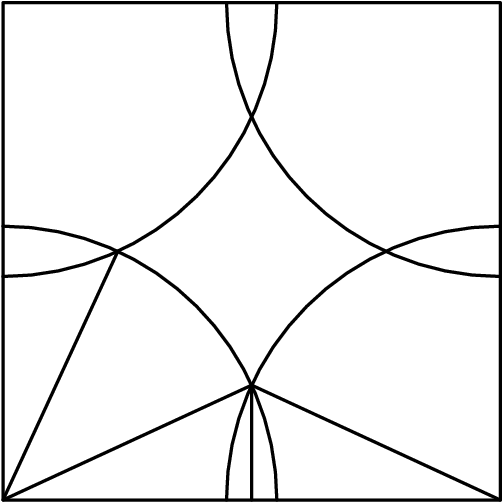
\includegraphics[width=7cm,height=7cm]{Sections/Files/11-2-1-img.png}
    \end{center}

    Since the arcs overlap, we split the area into four isosceles triangles and four arcs. The base angle of the triangle is $\arccos\left(\frac{1}{2r}\right)$
    and the height of the triangle is $\sqrt{r^2 - \frac{1}{4}}$ so the angle of the arc is $\frac{\pi}{2} - 2 \arccos\left(\frac{1}{2r}\right).$ Multiplying by
    four and plugging in $r = \sqrt{\frac{20}{21\pi}}$ we get
    $$P = \boxed{2 \sqrt{\dfrac{20}{21\pi} - \dfrac{1}{4}} + \dfrac{20}{21}\left(1 - \dfrac{4 \arccos\left(\frac{\sqrt{21 \pi}}{2\sqrt{20}}\right)}{\pi}\right)}.$$
\end{solution}\bigskip
        \newpage

        \subsubsection{WA is Required}
        \label{11.2.3}
        \SSbreak\\
\emph{Source: Original}\\
\emph{Proposer: \Ptan and \Pwen}\\
\emph{Problem ID: 156}\\
\emph{Date: 2021-03-10}\\
\emph{Difficulty: Easy}\\
\SSbreak

\SSpsetQ{
    Find the number of digits in the smallest positive integer $x$ such that there exists a positive integer $y$ such that $$2020x^{20^{21}} = 2021y^{21^{20}}.$$
}\bigskip

\begin{solution}\hfil\medskip
  
    Since $2020 = 2^2 \cdot 5 \cdot 101$ and $2021 = 43 \cdot 47$ we split $x, y$ into their prime factors; for $x$ to be minimal it should only have the necessary
    prime factors $2, 5, 43, 47, 101$. Let $x = 2^{x_1} \cdot 5^{x_2} \cdot 43^{x_3} \cdot 47^{x_4} \cdot 101^{x_5}$ and 
    $y = = 2^{y_1} \cdot 5^{y_2} \cdot 43^{y_3} \cdot 47^{y_4} \cdot 101^{y_5}$; we now can solve for the exponent of each prime independently. 
    Looking at the first equation we get $2 + 20^{21}x_1 = 21^{20}y_1$, or the equivalent $2 + 20^{21}x_1 \equiv 0 \pmod{21^{20}}$. 
    Let $I(a)$ be the modular inverse of $a$ mod $21^{20}$; then we have $x_1 \equiv -2 I\left(20^{21}\right) \pmod{21^{20}}$. 
    Solving similar equations for $x_2$ through $x_5$ we get $x_2 \equiv - I\left(20^{21}\right) \pmod{21^{20}}, x_3 = x_4 = I\left(20^{21}\right) \pmod{21^{20}}$.
    Putting this together, the number of digits is 
    $$\left\lfloor \left[21^{20} - 2I\left(20^{21}\right)\right] \log_{10}(2) + \left[21^{20} - I\left(20^{21}\right)\right] \log_{10}(505) + I\left(20^{21}\right) \log_{10}(2021) \right\rfloor + 1$$ $$= \boxed{835858264863808864064926340}.$$
\end{solution}\bigskip
        \newpage

        \subsubsection{Hard}
        \label{11.2.4}
        \SSbreak\\
\emph{Source: Original}\\
\emph{Proposer: \Ptan and \Pwen}\\
\emph{Problem ID: 157}\\
\emph{Date: 2021-03-11}\\
\emph{Difficulty: Hard}\\
\SSbreak

\SSpsetQ{
    Let $n$ be a power of $10$ greater than $10^{100}.$ A regular $n$-gon is inscribed in a unit circle, and a subset $S$ is chosen uniformly at random
    from the $2^n$ subsets of the polygon's vertices. If $A$ is the expected area of the convex hull of $S$, find $\pi - A$. 
}\bigskip

\begin{solution}\hfil\medskip
  
    By linearity of expectation, finding $\pi - A$ is the same as finding the expected area outside the convex hull inside the circle. So, we find the expected 
    area of a circular segment (the little cap thingy formed when you subtract the triangle off from the circular arc). Label the points $1$ through $n$ counterclockwise.
    Consider a circular segment that reaches from $1$ to $k$. The probability of getting such a circular segment from your point selection is $2^{-k}$, since
    the endpoints of the segment (vertices $1$ and $k$) need to be included while the $k - 2$ middle segments must be excluded. The area of such a circular segment
    is $\frac{(k - 1) \pi}{n} - \frac{1}{2}\sin\left(\frac{2 \pi (k - 1)}{n}\right)$ (yes, this covers segments with an obtuse angle as well - why?). Summing, we see that $k$ can range from 
    $2$ to $n$; however we need to correct for the edge cases where we select one or zero points, which contributes an expected area of $\frac{(n + 1)\pi}{2^n}$ (the whole circle).
    Since there are $n$ of each of the circular segments, our sum is $$n \sum_{k = 2}^{n} 2^{-k} \left[\dfrac{(k - 1)\pi}{n} - \dfrac{1}{2}\sin\left(\dfrac{2\pi(k - 1)}{n}\right)\right] + \dfrac{(n + 1)\pi}{2^n} = \dfrac{n}{2} \sum_{k = 1}^{n - 1} 2^{-k} \left[\dfrac{k\pi}{n} - \dfrac{1}{2}\sin\left(\dfrac{2k\pi}{n}\right)\right] + \dfrac{(n + 1)\pi}{2^n}$$
    and since $n$ is huge we can approximate $n - 1$ with $\infty$ and ignore the edge case (since $2^n$ grows way faster than $n$). The first sum of $k2^{-k}$ is an arithno-geometric
    series and evaluates to $2$; the second sum is the imaginary part of the sum of complex numbers $$\sum_{k = 1}^\infty \left(\dfrac{z}{2}\right)^k = \dfrac{z}{2} \cdot \dfrac{1}{1 - \frac{z}{2}} = \dfrac{z}{2 - z}$$
    where $z = \cos(a) + i \sin(a)$ and $a = \frac{2 \pi k}{n}$. Simplifying further, we have $$\dfrac{z}{2 - z} = \dfrac{\cos(a) + i\sin(a)}{2 - \cos(a) - i\sin(a)} = \dfrac{2 \cos(a) + 2i \sin(a)}{5 - 4\cos(a)}$$
    and scaling by a factor of 2 we have $$\sum_{k = 1}^\infty 2^{-k} \dfrac{1}{2}\sin\left(\dfrac{2k\pi}{n}\right) = \dfrac{\sin(a)}{5 - 4 \cos(a)}$$
    so putting it all together the expected value of $\pi - A$ is $$\pi - \dfrac{n \sin\left(\frac{2\pi}{n}\right)}{10 - 8 \cos\left(\frac{2\pi}{n}\right)}.$$
    Since $n$ is huge, we use the first two terms of the Taylor series to approximate our trigonometric functions; doing this we get $\boxed{\frac{26 \pi^3}{3n^2}}.$
\end{solution}\newpage

\begin{solution}[Write-up by \Pmano]\hfil\medskip
  
    $n$ is huge. Without loss of generality, one can assume that $S$ has at least 3 elements. We try to compute the expected area of one slice, i. e. 
    the part of a circular slice outside the polygon. Because of linearity of expectance, $n$ times this is $\pi-A$. Assume that, on the left of this circular 
    sector, the $k$-th vertex is the first one in $S$ and on the right, the $l$-th one. So the minimum case is when $k=l=0$ when two neighboring vertices are 
    both in $S$. The probability of one choice of $k,l$ happening is $\frac{1}{2^{k+1}2^{l+1}}$ The whole circular sector our slice lies in consists of 
    $k+l+1$ slices, so it has the area $\frac{\pi(k+l+1)}{n}$, the corresponding triangle has area $\frac{\sin(\frac{2\pi(k+l+1)}{n})}{2}$. As $n$ is huge, 
    we can sum to infinity without problems and  we are interested in $$n\sum_{k=0}^\infty \sum_{l=0}^\infty\frac{\frac{\pi(k+l+1)}{n}-\frac{\sin(\frac{2\pi(k+l+1)}{n})}{2}}{2^{k+1}2^{l+1}(k+l+1)}.$$ 
    Now, again, $n$ is huge so we can use the "fundamental theorem of engineering refined" without any concerns, i. e. that $\sin(x)=x-\frac{x^3}{6}$, 
    so we have: $$\frac{n}{24}\sum_{k=0}^\infty \sum_{l=0}^\infty \frac{\left(\frac{2\pi(k+l+1)}{n}\right)^3}{2^{k+l+1}(k+l+1)}=\frac{\pi^3}{3n^2}\sum_{k=0}^\infty \sum_{l=0}^\infty\frac{(k+l+1)^2}{2^{k+l+1}}=$$
    $$=\frac{\pi^3}{3n^2}\sum_{m=0}^\infty \sum_{k=0}^{m-1}\frac{m^2}{2^m}=\frac{\pi^3}{3n^2}\sum_{m=0}^\infty\frac{m^3}{2^m}.$$ So we ask WolframAlpha and we are surprised that there comes a nice answer, namely 26, a random integer. Where the 26 comes from is left to the reader. Finally, we are left with $\frac{26\pi^3}{3n^2}$. As we all know, the PSC consists of nice people, so they set $n$ and hence $n^2$ to a power of 10, so we now understand why they asked for the 2021st to 2030th significant figures, namely because this is just the 2021th to 2030th digits of $\frac{26\pi^3}{3}$, which is, according to WolframAlpha, $\boxed{8481609952}.$
\end{solution}\bigskip
        \newpage

        \subsubsection{hard}
        \label{11.2.5}
        \SSbreak\\
\emph{Source: Original}\\
\emph{Proposer: \Ptan and \Pwen}\\
\emph{Problem ID: 158}\\
\emph{Date: 2021-03-12}\\
\emph{Difficulty: Hard}\\
\SSbreak

\SSpsetQ{
    Let $N = 20^{21}.$ You play a game, starting with \$1. At each of $N$ steps, you can bet any nonnegative amount of money, $m$, up to how much you currently have, 
    and a computer flips a coin. If heads, you double your bet; if tails you lose it. \medskip

    However, before you start, you hack the computer, and you know that it will generate exactly $\frac{N}{2} + K$ heads. \medskip

    Suppose that you can guarantee yourself at least \$2021. If $K$ is minimal, find the leading five digits of $K$.
}\bigskip

\begin{solution}\hfil\medskip
  
    Let $g(h, t)$ denote the largest amount of money you can guarantee yourself if you start out with \$1. We claim that if we start out with \$$s$, then 
    the largest amount of money you can guarantee yourself is \$$sg(h, t)$. Clearly, $sg(h, t)$ is attainable, since we can use the same betting procedures
    when we did for \$1 and scale the bets proportionally by $s$. And if we can guarantee more than $sg(h, t)$ then dividing each of the bets by $s$ would mean
    that we can guarantee more than \$$g(h, t)$ if we started out with \$1, contradiction. (Intuitively, the amount of money you gain or lose in a bet is homogeneous
    with the amount of money you already have, so scalings are valid.) \medskip

    On our first step, suppose our optimal bet is \$$b$. If heads, the largest amount of money we can guarantee ourselves is $(1 + b)g(h - 1, t)$; if tails it is $(1 - b)g(h, t - 1)$
    and so $$g(h, t) = (1 + b)g(h - 1, t) = (1 - b)g(h, t - 1).$$ Noting that the sum of heads and tails decreased by 1, we seek $g(h, t)$ in terms of $g(h - 1, t)$ and $g(h, t - 1)$.
    Indeed, $$(1 + b) + (1 - b) = \dfrac{g(h, t)}{g(h - 1, t)} + \dfrac{g(h, t)}{g(h, t - 1)} \iff \dfrac{2}{g(h, t)} = \dfrac{1}{g(h - 1, t)} + \dfrac{1}{g(h, t - 1)}$$
    so $g(h, t)$ is the harmonic mean of $g(h - 1, t)$ and $g(h, t - 1)$. With the values $g(h, 0) = 2^h$ (go all-in every time) and $g(0, t) = 1$ (bet nothing every time)
    we get $$g(h, t) = \dfrac{2^{h + t}}{\sum_{k = 0}^t \binom{h + t}{k}} \iff \sum_{k = 0}^t 2^{-N}\dbinom{N}{k} \leq \dfrac{1}{2021}$$ after substituting relevant values.
    The last sum is a binomial distribution with $n = N$ and $p = q = \frac{1}{2}$; that is, think of $n$ independent events that can each take one of two outcomes:
    pass or fail, where each event passes with probability $p$ and fails with probability $q = 1 - p$. Letting $X$ be the random variable that denotes the number of events
    that passed, we see that our expression is equal to $\text{Pr}(X \leq t) \leq \frac{1}{2021}$; since $n$ is large we can approximate this binomial distribution
    by the normal distribution; in particular the quantity $\frac{X}{n}$ is normally distributed with mean $\mu = np = \frac{n}{2}$ and variance $\sigma^2 = \frac{pq}{n}$. 
    So, we want to find a $z$ such that $$\text{Pr}\left(\dfrac{X/n - \mu}{\sigma} \leq z\right) = \dfrac{1}{2021} \iff \dfrac{t}{n} = \sigma z + \mu \iff K = \abs(z)n \sigma$$
    and plugging $\frac{1}{2021}$ as our $p$-value into a $p$-value calculator we get that $K = \boxed{\left\lfloor 3.2946 \sqrt{0.25 \cdot 20^{21}} \right\rfloor}$.
\end{solution}\bigskip
        \newpage

\ihead{\footnotesize\bfseries\sffamily{Return to Normalcy (Season 12)}}
\section{Return to Normalcy (Season 12)}

    \ihead{\footnotesize\bfseries\sffamily{Return to Normalcy (Season 12), Week 1}}
    \subsection{Week 1}
        
    \subsubsection{Quadrilateral Perimeter}
	\label{12.1.1}
	\SSbreak\\
\emph{Source: Folklore}\\
\emph{Proposer: \Pflame}\\ %\Pchan \Pbrain \Pss
\emph{Problem ID: 161}\\
\emph{Date: 2021-03-29}\\
\emph{Difficulty: Beginner}\\
\SSbreak

\SSpsetQ{
	Let $ABCD$ be a convex quadrilateral satisfying \[AB = 1, BC = 6, CD = 18, AC \perp BD.\] Find its perimeter.
	%Put Problem Here
}\bigskip

\begin{solution}\hfil\medskip
	
	Let $E$ be the intersection of the diagonals of $ABCD$. Then $AB^2 + CD^2 = AE^2 + EB^2 + CE^2 + ED^2$ and $BC^2 + DA^2 = BE^2 + EC^2 + DE^2 + EA^2$ by the Pythagorean Theorem. This implies that $AB^2 + CD^2 = BC^2 + DA^2$, or $1^2 + 18^2 = 6^2 + x^2$. Solving yields $x=17$, so the answer is $1+18+6+17=\boxed{42}$.
	%Put sol here
\end{solution}\bigskip

	\newpage

    \subsubsection{Involution Convolution}
	\label{12.1.2}
	\SSbreak\\
\emph{Source: \Casmc, 2019 Q30}\\
\emph{Proposer: \Pbrain}\\
\emph{Problem ID: 162}\\
\emph{Date: 2021-03-30}\\
\emph{Difficulty: Easy}\\
\SSbreak
 
\SSpsetQ{

A function \(f\), defined on the set of positive integers, has \(f(1)=2\) and \(f(2)=3\). Also \(f(f(f(n)))=n+2\) if \(n\) is even and \(f(f(f(n)))=n+4\) if \(n\) is odd. What is \(f(777)\)?

}\bigskip

\begin{solution}\hfil\medskip
Observe that \(777 = 4 \times 194 + 1\). Thus
\begin{align*}
	f(777) &= f(f^{194 \times 3}(1)) \\
	&= f^{194 \times 3} (f(1)) \\
	&= f^{194 \times 3} (f(2)) \\
	&= 2 + 194 \times 2 \\
	&= \boxed{390}
\end{align*}

\end{solution}\bigskip

	\newpage

    \subsubsection{Coordinates without Bash}
	\label{12.1.3}
	\SSbreak\\
\emph{Source: \Cop}\\
\emph{Proposer: \Pdenial}\\
\emph{Problem ID: 163}\\
\emph{Date: 2021-03-31}\\
\emph{Difficulty: Medium}\\
\SSbreak

\SSpsetQ{
	A circle of radius 1 is centred at \((1,1)\). Points \(A\) and \(B\) have co-ordinates \((a, 0)\) and \((0, b)\), with \(a,b > 2\). If \(AB\) is tangent to the circle, what is the sum of all possible integer values of \(a\) and \(b\)?
}\bigskip

\begin{solution}[Solution by \Pdenial]\hfil\medskip
	
	Let \(O, C, D\) and \(E\) have coordinates \((1,1), (0,0), (0,1)\) and \((1,0)\) respectively, and let the point of tangency of \(AB\) with the circle be \(F\).\\
Note since \(O\) and \(D\) have the same \(y\) co-ordinate \(OD\) is parallel to the \(x\)-axis and hence perpendicular to the \(y\)-axis. Since \(D\) is also on the \(y\)-axis, \(BC\) is tangent to the circle at \(D\). Similarly, \(O\) and \(E\) have the same \(x\) co-ordinate, so \(OE\) is parallel to the \(y\)-axis and hence perpendicular to the \(x\)-axis. Since \(E\) is also on the \(x\)-axis, \(AC\) is tangent to the circle at \(E\).\\
Since the tangents to a circle from a point have equal length, \(BF = BD\) and \(FA = AE\). Summing, \(BF + FA = BD + AE\), so \(BA = (BC - CD) + (AC - CE) = (b-1) + (a-1) = a + b - 2\), giving \(AB^2 = (a+b-2)^2\). However, since \(\angle ACB = 90^{\circ}\), by Pythagoras' theorem, \(AB^2 = a^2 + b^2\), and so we have
\begin{equation*}a^2 + b^2 = (a+b-2)^2\end{equation*}
\begin{equation*}a^2 + b^2 = a^2 + b^2 + 4 + 2ab - 4a - 4b\end{equation*}
\begin{equation*}0 = 2ab - 4a - 4b + 4\end{equation*}
\begin{equation*}ab - 2a - 2b + 2 = 0\end{equation*}
\begin{equation*}ab - 2a - 2b + 4 = 2\end{equation*}
\begin{equation*}(a-2)(b-2) = 2\end{equation*}
However, \(a,b > 2\), so if \(a\) and \(b\) are integers, then \(a-2\) and \(b-2\) are positive integers and hence must both be positive factors of \(2\). Since 2 is primes, its only factorisation is as \(2 = 2 \times 1\), so either \(a-2 = 2\) and \(b-2 = 1\) or \(a-2 = 1\) and \(b-2 = 2\). Hence the possible integer values of \(a\) and \(b\) are \((a,b) = (3,4)\) or \((4,3)\). Giving a final answer of \fbox{14}
\end{solution}\bigskip

	\newpage

    \subsubsection{April Fool's}
	\label{12.1.4}
	\SSbreak\\
\emph{Source: brain}\\
\emph{Proposer: \Pbrain}\\ %\Pchan \Pbrain \Pss
\emph{Problem ID: 164}\\
\emph{Date: 2021-04-01}\\
\emph{Difficulty: Random}\\
\SSbreak

\SSpsetQ{
	How many official solves will this Sunday's problem get?
	%Put Problem Here
}\bigskip

\begin{solution}\hfil\medskip
	
	Answer: \fbox{21} \medskip
    Five people managed to guess 21.
	%Put sol here
\end{solution}\bigskip
	\newpage
	
	\subsubsection{FE}
	\label{12.1.5}
	\SSbreak\\
\emph{Source: 2011 Kosovo TST \#5}\\
\emph{Proposer: \Paiya}\\ %\Pchan \Pbrain \Pss
\emph{Problem ID: 165}\\
\emph{Date: 2021-04-02}\\
\emph{Difficulty: Hard}\\
\SSbreak

\SSpsetQ{
	There exist functions $f: \mathbb{R} \setminus \{1, -1\} \to \mathbb{R}$ such that the following holds:
    $$f\left(\dfrac{x - 3}{1 + x}\right) + f\left(\dfrac{x + 3}{1 - x}\right) = x$$
    Then the average value of $$\sum_{k = 2}^{100} \dfrac{f(k)}{k}$$ can be 
    expressed in the form $\frac{m}{n}$, where $m, n$ are relatively prime integers and $n$ is positive. Find $100m + n$. \medskip

    (For example, if the solutions to that FE were $f(x) \equiv 0$ and $f(x) \equiv -x^2$ then the average value of that sum would be $-\frac{5049}{2}$
    and your answer would be $2 - 504900 = -504898$.)\medskip

    \begin{center}
        \textit{(A four-function calculator may be used.)}
    \end{center}
	%Put Problem Here
}\bigskip

\begin{solution}\hfil\medskip
	
    The unique function can be found using \href{https://artofproblemsolving.com/community/c6h403803}{AoPS solutions}; then note that $\frac{f(x)}{x}$ can be decomposed into partial fractions and so the sum telescopes.
    Answer: \fbox{-13243675}
	%Put sol here
\end{solution}\bigskip

	\newpage

	\subsubsection{So this is where American problem quality went}
	\label{12.1.6}
	\SSbreak\\
\emph{Source: 2012 AIME II \#15}\\
\emph{Proposer: \Paiya}\\ %\Pchan \Pbrain \Pss
\emph{Problem ID: 166}\\
\emph{Date: 2021-04-03}\\
\emph{Difficulty: Challenging}\\
\SSbreak

\SSpsetQ{
	Triangle $PQR$ is inscribed in circle $\Gamma$ with $PQ=5$, $QR=7$, and $RP=3$. The bisector of angle $P$ meets side $\overline{QR}$ at $X$ and circle $\Gamma$ at a second point $Y$. Let $\gamma$ be the circle with diameter $\overline{XY}$. Circles $\Gamma$ and $\gamma$ meet at $Y$ and a second point $Z$. Then $PZ^2 = \frac{m}{n}$, where $m$ and $n$ are relatively prime positive integers. Find $100m+n$. 
	%Put Problem Here
}\bigskip

\begin{solution}\hfil\medskip
	
	\href{https://artofproblemsolving.com/wiki/index.php/2012_AIME_II_Problems/Problem_15}{AoPS Solutions} Answer: \fbox{90019}
	%Put sol here
\end{solution}\bigskip


	\newpage

	\subsubsection{640 Generators of Pain}
	\label{12.1.7}
	\SSbreak\\
\emph{Source: 2015 PUMAC Number Theory A7}\\
\emph{Proposer: \Paiya}\\ %\Pchan \Pbrain \Pss
\emph{Problem ID: 167}\\
\emph{Date: 2021-04-04}\\
\emph{Difficulty: Challenging}\\
\SSbreak

\SSpsetQ{
	For positive integers $n$, let $s(n)$ be the sum of the $n$-th powers of the primitive roots mod 1601. Find the number of positive integers $n \leq 2021$ such that $s(n)$ is divisible by 1601.
	%Put Problem Here
}\bigskip

\begin{solution}\hfil\medskip
	
	First, some lemmas about orders and generators (skip if you think people should know this already): \medskip
	
	\textit{Lemma 1.} The order of $g^n$, where $g$ is a generator mod prime $p$, is $d = \frac{p - 1}{(n, p - 1)}$ where $(a, b)$ is the greatest common divisor function. 
	
	\textbf{Proof.} Since $g^{nd} \equiv 1 \pmod{p}$ we have $p - 1 | nd$ so $\frac{p - 1}{(n, p - 1)} | d$. Since $d$ is defined to be minimal we have $d = \frac{p - 1}{(n, p - 1)}$. \medskip
	
	\textit{Lemma 2.} The number of residues mod $p$ with order $d$ is $\varphi(d)$, where $\varphi$ is Euler's totient function. 
	
	\textbf{Proof.} We want to find the number of positive integers $k$ such that $d$ is the least positive integer for which $\left(g^{k\frac{p - 1}{d}}\right)^d \equiv 1 \pmod{p}$. For that to be satisfied, $k$ and $d$ cannot share any common factors; otherwise $\left(g^{k\frac{p - 1}{d}}\right)^{\frac{d}{(k, d)}} \equiv 1 \pmod{p}$. Also, since $d$ is the order only $k < d$ generate unique residues. The number of positive integers $k$ less than $d$ such that $(d, k) = 1$ is $\varphi(d)$.\medskip
	
	Let $p = 1601$ since 1601 is prime. The order of $g^n$ mod $p$ is $d = \frac{p - 1}{(n, p - 1)}$; also each of the $\varphi(p - 1)$ terms in $s(n)$ can take only one of $\varphi\left(\frac{p - 1}{(n, p - 1)}\right)$ residues with order $d$ mod $p$. By symmetry, each residue of order $d$ is represented the same amount of times in $s(n)$. Now let $r(d)$ be the sum of the residues with order $d$ mod $p$, so $$s(n) = \dfrac{\varphi(p - 1)}{\varphi\left(\frac{p - 1}{(n, p - 1)}\right)} r(d).$$ Notice that the ratio of totient functions is less than $p$, so if $p | s(n)$ then $p | r(d)$. 
	
	Consider a residue $a$ with order $d$; then $p| a^d - 1 = (a - 1)\left(a^{d - 1} + a^{d - 2} + \cdots + 1\right)$ and since $a < p$ we have $a^{d - 1} + a^{d - 2} + \cdots + 1 \equiv 0 \pmod{p}$. Remembering $\sum_{d|n} \varphi(d) = n$ we conjecture that that sum is $\sum_{e|d} r(e) \equiv 0 \pmod{p}$; indeed we can treat $a$ like the ""generator"" of the residue class of order $d$ mod $p$ and follow the steps of Lemma 2. \medskip
	
	\textit{Claim.} $r(d) \equiv 0 \pmod{p}$ if and only if $d$ is not squarefree. \medskip
	
	As with any divisor sum, we try products of primes: $r(1) = 1$, $r(p) = -1, r(pq) + r(p) + r(q) + 1 \equiv 0 \iff r(pq) = 1$ and induct on $k$ to get $r\left(p_1p_2 \cdots p_k\right) = (-1)^k$. Notice $r\left(p^2\right) + r(p) + r(1) \equiv 0 \iff r\left(p^2\right) \equiv 0$; a similar induction argument yields $r(d) \equiv 0$ if $d$ is not squarefree. 
	
	We are homeward-bound: for $d = \frac{p - 1}{(n, p - 1)} = \frac{1600}{(n, 1600)}$ to be squarefree we must have $2^5 \cdot 5 = 160 | n$. We have $2021 - \left\lfloor \frac{2021}{160} \right\rfloor = \boxed{2009}$ such $n$.
	%Put sol here
\end{solution}\newpage

\begin{solution}[Solution by \Pmano]\hfil\medskip
	
	$n$-th powers of roots is something that polynomials can handle very well. The definition of order, $g^{p - 1} \equiv 1 \pmod{p} \iff g^{p - 1} - 1 \equiv 0 \pmod{p}$,
	motivates us to look at the polynomial $x^{p - 1} - 1$. Which integers $g$ satisfy $g^{p - 1} - 1 \equiv 0 \pmod{p}$ but not $g^d - 1 \equiv 0 \pmod{p}$ for all 
	$d < p$? We claim that the polynomial in question is $\Phi_{p - 1}(x)$, the $p - 1$-th cyclotomic polynomial. (If you don't know what a cyclotomic polynomial is, google.)
	While it is easy to compute $\Phi_p(x)$, computing $\Phi_{p - 1}(x) = \Phi_{1600}(x)$ will be harder. Using $\Phi_n(x) = \prod_{d|n} \Phi_d(x)$ we can 
	get $$x^{p^k} - 1 = \left(x^{p^{k - 1}} - 1\right) \Phi_{p^k}(x) = \left[\left(x^{p^{k - 1}}\right)^p - 1\right] \iff \Phi_{p^k}(x) = \sum_{h = 0}^{p - 1} x^{hp^{k - 1}}.$$
	We now turn our attention to $\Phi_{p^kn}(x)$ for $(p, n) = 1$. Note that $\Phi_n\left(x^{p^k}\right)$ has roots of unity $\exp\left(\frac{\tau m}{p^kn}\right)$
	where $\left(m, p^kn\right) = 1, p, \cdots , p^k$. However, we want only $\left(m, p^kn\right) = 1$; note then, that $\Phi_n\left(x^{p^{k - 1}}\right)$ has roots of unity
	$\exp\left(\frac{\tau m}{p^{k - 1}n}\right) = \exp\left(\frac{\tau pm}{p^kn}\right)$ where $\left(m, p^{k - 1}n\right) = 1, p, \cdots , p^{k - 1}$ so $\left(pm, p^kn\right) = p, p^2, \cdots , p^k$
	and so $$\Phi_{p^kn}(x) = \dfrac{\Phi_n\left(x^{p^k}\right)}{\Phi_n\left(x^{p^{k - 1}}\right)}.$$
	Thus, we have $\Phi_{25}(x) = 1 + x^5 + x^{10} + x^{15} + x^{20} = \frac{x^{25} - 1}{x^5 - 1}$ and so 
	$$\Phi_{1600}(x) = \Phi_{2^6 \cdot 25}(x) = \dfrac{\Phi_{25}\left(x^{64}\right)}{\Phi_{25}\left(x^{32}\right)} = \dfrac{x^{800} + 1}{x^{160} + 1} = 1 - x^{160} + x^{320} - x^{480} + x^{640}$$
	where we have omitted two difference of squares factorizations since $2^6 = 2^5 \cdot 2$ and so $x^{2^6} = \left(x^{2^5}\right)^2$. \medskip

	\textit{Newton's Sums.} Let $r_1, r_2, \cdots , r_n$ be the roots of polynomial $a_nx^n + a_{n - 1}x^{n - 1} + \cdots + a_0x^0$, and let $s_k = \sum_{i = 1}^n r_i^k$.
	Then $\sum_{i = 0}^n a_{n - i}s_{k - i} = 0$ if $k \geq n$ and $(-1)^kka_{n - k} + \sum_{i = 0}^{k - 1} (-1)^ia_{n - i}s_{k - i} = 0$ if $k < n$. \medskip

	Using Newton's sums, it becomes clear that the only nonzero terms of $s(n)$ happen when $160|n$; our answer is thus \fbox{2009}.
\end{solution}\newpage

\begin{solution}[Solution by \Pmonke]\hfil\medskip
	
	Let $g$ be a known generator mod $p$. Note that if $(k, p - 1) = 1$ then $g^k$ is also a generator mod $p$. We have $p - 1 = 1600 = 2^6 \cdot 5^2$; 
	the integers not coprime to $p - 1$ are either multiples of $2$, multiples of $5$, or multiples of $10$. Now observe that $$\sum_{a = 1}^{1600} g^a$$
	sums over all powers of $g$; however since we only want coprime powers we need to subtract off powers that are multiples of $2$ or $5$. Using inclusion-exclusion, 
	this is $$s(n) = \sum_{a = 1}^{1600} g^{an} - \sum_{b = 1}^{800} g^{bn} - \sum_{c = 1}^{320} g^{cn} + \sum_{d = 1}^{160} g^{dn}$$
	which can be rewritten and re-summed as $$\dfrac{g^{1601n} - 1}{g^n - 1} - \dfrac{g^{1602n} - 1}{g^{2n} - 1} - \dfrac{g^{1605n} - 1}{g^{5n} - 1} + \dfrac{g^{1610n} - 1}{g^{10n} - 1} \equiv 0 \pmod{p}$$
	with a small catch: if any of $g^n, g^{2n}, g^{5n}, g^{10n}$ is $1$ the geometric series sum represntation fails, and it is easy to see that $s(n)$ will not be $0$ mod $p$ 
	in that case. Thus, the cases where $s(n) \not\equiv 0 \pmod{p}$ is when $160|n$; our answer is then \fbox{2009}.
\end{solution}\bigskip
	\newpage

    \ihead{\footnotesize\bfseries\sffamily{Return to Normalcy (Season 12), Week 2}}
    \subsection{Week 2}

    \subsubsection{Even Numbers with Restrictions}
	\label{12.2.1}
	\SSbreak\\
\emph{Source: AMC10, 2011 Q13}\\
\emph{Proposer: \Pss}\\
\emph{Problem ID: 168}\\
\emph{Date: 2021-04-05}\\
\SSbreak

\SSpsetQ{
How many even integers are there between 200 and 700 whose digits are all different and come from the set \(\{1,2,5,7,8,9\}\)
}\bigskip

\begin{solution}\hfil\medskip

\href{https://artofproblemsolving.com/wiki/index.php/2011_AMC_10A_Problems/Problem_13}{AoPS Solutions} Answer: \fbox{12}
\end{solution}\bigskip

	\newpage
    
    \subsubsection{Enjoyable}
	\label{12.2.2}
	\SSbreak\\
\emph{Source: Canadian Open Mathematics Challenge 2018}\\
\emph{Proposer: \Pnjoy}\\ %\Pchan \Pbrain \Pss
\emph{Problem ID: 169}\\
\emph{Date: 2021-04-06}\\
\emph{Difficulty: Beginner}\\
\SSbreak

\SSpsetQ{
	Five \emph{distinct} integers $e, n, j, o, y$ are such that \[e\cdot n \cdot j \cdot o \cdot y = 775.\]
	Find \( e + n + j + o + y\). 
	%Put Problem Here
}\bigskip

\begin{solution}\hfil\medskip
	
	Note that \(775 = 5^2 \cdot 31\). In particular, this means that the only way to factor into 5 distinct integers is to have \( \{e, n, j, o, y\} = \{1, -1, 5, -5, 31\} \), giving us a sum of \(1 - 1 + 5 - 5 + 31 = \boxed{31}\). 
	%Put sol here
\end{solution}\bigskip


	\newpage

    \subsubsection{Isosceles Tetrahedron}
	\label{12.2.3}
	\SSbreak\\
\emph{Source: IMTS Year 1991 R4 Problem 5 (modified)} \\
\emph{Proposer: \Pflame}\\ %\Pchan \Pbrain \Pss
\emph{Problem ID: 170}\\
\emph{Date: 2021-04-07}\\
\emph{Difficulty: Easy}\\
\SSbreak

\SSpsetQ{
	Paper $\triangle XYZ$ has $XY=69$, $YZ=91$, $ZX=100$. Let $A$, $B$, $C$ be the midpoints of $\overline{XY}$, $\overline{YZ}$, $\overline{ZX}$ respectively. The triangle is folded about $AB$, $BC$, and $CA$ to form a tetrahedron $\mathcal{T}$. What is the volume of $\mathcal{T}$?
	%Put Problem Here
}\bigskip

\begin{solution}\hfil\medskip
	
	\href{https://artofproblemsolving.com/community/q2h54423p339658}{AoPS Solution using Pythagorean Theorem} \medskip

	We will prove that in an isosceles tetrahedron (opposite edges have the same length) with edge lengths $a, b, c$, the volume of such a tetrahedron is 
	$$V = \sqrt{\dfrac{\left(a^2 + b^2 - c^2\right)\left(a^2 - b^2 + c^2\right)\left(-a^2 + b^2 + c^2\right)}{72}}.$$
	First, note that every "acute" tetrahedron can be inscribed in a parallepiped prism, with each edge being a diagonal of each face (see \href{https://www.cut-the-knot.org/triangle/TetrahedronInParallelepiped.shtml}{here} for a picture). 
	This is because there is exactly one pair of parallel planes that pass through each pair of opposite edges 
	(since opposite edges are skew lines, so you can't just rotate the planes wrt the axis of one edge). 
	Also note that since opposite edges are skew, this means that the opposite edges take up the two different diagonals of their inscribed parallelogram face.
	Since opposite edges are equal in an isosceles tetrahedron, this implies that the parallelogram has equal diagonals, implying that it's a rectangle,
	and the circumscribed parallepiped is actually a rectangular prism. Letting $x, y, z$ represent the edges of the prism, we have
	$$x^2 + y^2 = a^2, y^2 + z^2 = b^2, z^2 + x^2 = c^2 \iff \left(x^2, y^2, z^2\right) = \left(\dfrac{-a^2 + b^2 + c^2}{2}, \dfrac{a^2 - b^2 + c^2}{2}, \dfrac{a^2 + b^2 - c^2}{2}\right)$$
	and now we claim that the volume of the prism is three times the volume of the tetrahedron; indeed the space outside the inscribed tetrahedron but inside the prism
	is composed of three congruent right-angle-cornered tetrahedra, each with volume $\frac{xyz}{6}$. 
	Thus $$V = \dfrac{xyz}{3} = \sqrt{\dfrac{\left(a^2 + b^2 - c^2\right)\left(a^2 - b^2 + c^2\right)\left(-a^2 + b^2 + c^2\right)}{72}}.$$
	
	Answer: \(\boxed{7605}\)
	%Put sol here
\end{solution}\bigskip

	\newpage

    \subsubsection{Sums of powers of 2 but weird}
	\label{12.2.4}
	\SSbreak\\
\emph{Source: 2018 PUMAC Algebra A5}\\
\emph{Proposer: \Pchan}\\ %\Pchan \Pbrain \Pss
\emph{Problem ID:}\\
\emph{Date: }\\
\emph{Difficulty: Medium}\\
\SSbreak

\SSpsetQ{
	For $k \in \{0, 1, \dots, 9\}$, let $\epsilon_k \in \{-1, 1\}$. Find the minimum possible value of \[\sum_{i=1}^9 \sum_{j=0}^{i-1} \epsilon_i \epsilon_j 2^{i+j}.\]
	%Put Problem Here
}\bigskip

\begin{solution}\hfil\medskip
	
	\href{https://static1.squarespace.com/static/570450471d07c094a39efaed/t/5bfb8c2570a6ad835e78ca0d/1543212069335/Algebra+A+Solutions.pdf}{Solution PDF} Answer: \fbox{174762}
	%Put sol here
\end{solution}\bigskip

	\newpage

	\subsubsection{"D4 I swear"}
	\label{12.2.5}
	\SSbreak\\
\emph{Source: 2012 Winter OMO 43}\\
\emph{Proposer: \Paiya}\\ %\Pchan \Pbrain \Pss
\emph{Problem ID: 172}\\
\emph{Date: 2021-04-09}\\
\emph{Difficulty: Hard}\\
\SSbreak

\SSpsetQ{
	Let $p = 2017$. An integer $n$ is uniformly and randomly selected between 1 and $\left(p^p - 1\right)!$ inclusive. The probability that $n^n - 1$ is divisible by $p$ can be written in the form $\frac{m}{n},$ where $m$ and $n$ are relatively prime positive integers. Find $100m + n$. 
	%Put Problem Here
}\bigskip

\begin{solution}\hfil\medskip
	
	Fix an order $d$; we find the probability that $d|n$ and $n$ has order $d$ mod $p$. Since the first probability involves $n$'s behavior mod $d$ and the second $n$'s behavior mod $p$ and $\gcd(d, p - 1) = 1$, these events are independent. Since our interval is from $1$ to $\left(p^p - 1\right)!$, each residue mod $p$ and mod $p - 1$ (and thus mod $d$) appears the same amount of times. Thus, our first event happens with probability $\frac{1}{d}$ and our second with probability $\frac{\varphi(d)}{p}$, where we have used the fact that there are exactly $\varphi(d)$ residues with order $d$ mod $p$. It remains to sum this probability over all possible values of $d$, or, $$P = \dfrac{1}{p} \sum_{d|p - 1} \dfrac{\varphi(d)}{d} = \dfrac{1}{p} s(p - 1),$$ where $s(n) = \sum_{d|n} \frac{\varphi(d)}{d}$. As with all divisor sums, we test with $n = p, p^2, pq$: $s(p) = 1 + \frac{p - 1}{p} = 2 - \frac{1}{p}$, $s\left(p^2\right) = s(p) + \frac{p(p - 1)}{p^2} = 3 - \frac{2}{p}$, $s(pq) = 1 + \frac{p - 1}{p} + \frac{q - 1}{q} + \frac{(p - 1)(q - 1)}{pq} = \left(2 - \frac{1}{p}\right)\left(2 - \frac{1}{q}\right)$; we conjecture that $s(n)$ is multiplicative. Indeed, letting $n = p_1^{e_1}p_2^{e_2} \cdots p_k^{e_k}$, two induction arguments, one on $k$ and one on $e$, yields $$s(n) = \prod_{i = 1}^k e_i + 1 - \dfrac{e_i}{p_i}$$ so $s(p - 1) = s(2016) = \left(6 - \frac{5}{2}\right)\left(3 - \frac{2}{3}\right)\left(2 - \frac{1}{7}\right) = \frac{91}{6}$ so $P = \frac{91}{6p} \iff \boxed{21202}$. 
	%Put sol here
\end{solution}\bigskip

	\newpage

    \subsubsection{"change the point distribution up so weekends don't carry people"}
	\label{12.2.6}
	\SSbreak\\
\emph{Source: Unknown}\\
\emph{Proposer: \Paiya}\\ %\Pchan \Pbrain \Pss
\emph{Problem ID: 173}\\
\emph{Date: 2021-04-10}\\
\emph{Difficulty: Challenging}\\
\SSbreak

\SSpsetQ{
    2021 coplanar lines intersect at $2021 \cdot 1010$ distinct points $K_1, K_2, \cdots K_{2021 \cdot 1010}$. Let $P$ be a point in the plane not on any of the lines.
    We call an intersection point $K$ $k$\textit{-reachable} if segment $PK$ intersects at most $k$ lines, excluding the intersection point at $K$.
    If $1999420$ points are $k$-reachable, find the largest possible value of $k$.
}\bigskip

\begin{solution}\hfil\medskip
    
    First note that no two of these 2021 lines are parallel and no three of them are concurrent, otherwise the number of intersection points
    would be less than $2021 \cdot 1010$. After some playing around with small cases of $n$, we claim that the minimal number of $k$-reachable points among $n$ such lines is $\binom{k + 2}{2}$. 
    The base case $k = 0$ for arbitrary $n$ is trivial. Assume the condition holds for $k - 1$ and $n - 1$. 
    Consider the line with minimal distance to $P$. Label its intersection points $P_1, P_2, \cdots , P_n$ where $KP_1 < KP_2 < \cdots < KP_n$. 
    Among these $n$ points, at least $k$ of them are $k$-reachable (consider the worst-case scenario where $P$ is on the left of all the intersection points).
    Now remove this line; among the remaining points there are at least $\binom{k + 1}{2}$ $(k - 1)$-reachable points. 
    When we add the line back, those $(k - 1)$-reachable points become $k$-reachable points (any point $Q$ in that set either had $PQ$ cross that deleted line or not).
    It remains to bound $\binom{k + 2}{2} \approx (k + 2)^2/2$. Noticing $1999420 \approx 1999200 = 1400 \cdot 1428 \approx 1414^2$ and $\sqrt{2} = 1.414$, we have
    $2 \cdot 1414^2 \approx 2000^2 \iff 1999420 > \binom{2000}{2}$. Our answer is $\boxed{1998}$. 
\end{solution}\bigskip
	\newpage

	\subsubsection{Notice me, sqing-senpai}
	\label{12.2.7}
	\SSbreak\\
\emph{Source: 2019 China Mathematical Olympiad P1, Modified}\\
\emph{Proposer: \Paiya}\\ %\Pchan \Pbrain \Pss
\emph{Problem ID: 174}\\
\emph{Date: 202-04-11}\\
\emph{Difficulty: Challenging}\\
\SSbreak

\SSpsetQ{
	Let $\left(a_1, a_2, a_3, a_4, a_5, a_6\right)$ be reals no less than $-2020$ that sum to $2021$. 
    Let $M$ and $m$ be the maximum and minimum, respectively, of the function 
    $$f\left(a_1, a_2, a_3, a_4, a_5, a_6\right) = \prod_{k = 1}^6 \left(a_k + a_{k + 1}\right),$$ where indices are taken modulo $6$,
    and let $N$ and $n$ be the number of ordered pairs which maximize and minimize $f$, respectively.
    Find $\left\lfloor \ln(-Mm) \right\rfloor + N + n$. \medskip

    \begin{center}
        \textit{(A scientific calculator may be used.)}
    \end{center}
	%Put Problem Here
}\bigskip

\begin{solution}\hfil\medskip
	
	We switch variables to $(a, b, c, d, e, f)$ for sake of legibility. WLOG $a$ is maximal; therefore $a + b, f + a \geq 0$. 
    We solve for the minimum first, as that is less painful. Negative values are possible, which correspond to either one or three negative factors.
    If there is only one negative factor, then there are at least two positive variables less than $2021$; flipping their signs and increasing
    the value of the greatest two variables accordinaly produces a product greater in absolute value, so we want three negative factors.
    Let $a + b, b + c, c + a < 0$ (the factor adjacency really does matter as we'll see in a bit). Applying AM-GM twice, once to the positive factors and once to the negative, we have
    $$f \leq \left(\dfrac{-a - 2b - 2c - d}{3}\right)^3\left(\dfrac{d + 2e + 2f + a}{3}\right)^3$$
    and since $d + 2e + 2f + a = 2 \cdot 2021 - (a + 2b + 2c + d)$ we see that the maximum occurrs when $a + 2b + 2c + d$ is minimized;
    this happens at $a = b = c = d = -2020$ and $e = f = \frac{10101}{2}$. Note that the variables with coefficient $2$ must be different variables; in other words, the three factors we chose to be negative matters.
    In esssence, the two positive terms have to be next to each other, so $n = 6$.\medskip

    Now for the maximum. By the same argument, having all positive factors does not yield a maximal configuration; therefore there are either two or four negative factors.
    Applying AM-GM in the same fashion (once to the positive factors and once to the negative factors) we get that the equality case is one of four
    and that the maximal configuration happens when all the variables in the negative terms are equal to $-2020$. Thus, four negative factors is optimal;
    this happens at $a = b = c = d = e = -2020$ and $f = 12121$ and $N = 6$.\medskip

    Our answer is $$\left\lfloor \ln\left(2^5 \cdot 2020^6 \cdot 6061^2 \cdot 10101^3\right) \right\rfloor + 6 + 6 = \boxed{113}.$$
	%Put sol here
\end{solution}\bigskip

	\newpage

\ihead{\footnotesize\bfseries\sffamily{Quality Uncontrol (Season 13)}}
\section{Quality Uncontrol (Season 13)}

    \ihead{\footnotesize\bfseries\sffamily{Quality Uncontrol (Season 13), Week 1}}
    \subsection{Week 1}
        
    \subsubsection{Choi's Balls}
	\label{13.1.1}
	
\SSbreak\\
\emph{Source: \Cfolk}\\
\emph{Proposer: \Pss}\\
\emph{Problem ID: 175}\\
\emph{Date: 2021-04-19}\\
\emph{Difficulty: Beginner}\\
\SSbreak
 
\SSpsetQ{
    Choi has three types of counters, coloured red, blue and green which she must place on a numberline consisting of the numbers 1,2 and 3.
    
    In how many ways can she arrange the counters such that no red counter is directly to the left of a blue counter?
}\bigskip

\begin{solution}\hfil\medskip

    There are \(3^3\) ways of arranging the counters without restrictions and \(2\cdot3=6\) ways to pick the red counter being next to the blue counter, thus we have \(3^3-6=\fbox{21}\) total ways.

\end{solution}\bigskip

	\newpage

    \subsubsection{Biscriminant}
	\label{13.1.2}
	
\SSbreak\\
\emph{Source: \Cfolk}\\
\emph{Proposer: \Pss}\\
\emph{Problem ID: 176}\\
\emph{Date: 2021-04-20}\\
\emph{Difficulty: Beginner}\\
\SSbreak
 
\SSpsetQ{
    Given that for \(f(x)=x^2+bx+7\) and \(f(x)\ne -18\), the possible values of \(b\) can be written in the form \(x<b<y\). What is the value of \(x^2+y^2\)?
}\bigskip

\begin{solution}\hfil\medskip

    We want to find the values of be such that \(x^2+bx+7=-18\) has no real solutions. By taking the discriminant, we see that we require \(b^2-4\cdot25<0\iff -10<b<10\). Therefore our answer is \fbox{200}.

\end{solution}\bigskip

	\newpage
    
    \subsubsection{\Cmac  2012 P6}
	\label{13.1.3}
	\SSbreak\\
\emph{Source: 2012 IMOK Maclaurin Problem 6}\\
\emph{Proposer: \Palch}\\ %\Pchan \Pbrain \Pss
\emph{Problem ID: 177}\\
\emph{Date: 2021-04-21}\\
\emph{Difficulty: Easy}\\
\SSbreak
 
\SSpsetQ{
	Three different positive integers have the property that each of them divides the sum of the other two. Let S be a possible set of three such integers. What is the smallest possible integer in S such that the sum of the three integers in S is greater than 2021? 
	%Put Problem Here
}\bigskip

\begin{solution}\hfil\medskip
	
	Let the three integers be \(a, b, c\) where \(0 < a < b < c\). This means that \(a + b < 2c\) and because \(c | a + b\) $\rightarrow$ \(a + b = c\). We also know that \(b|a + c \) $\rightarrow$ \(b|2a + b\) $\rightarrow$ \(b|2a\). \(b > a\) meaning that \(b = 2a\) and this gives us the solutions \((a, 2a, 3a)\). This gives that the sum of the integers in S is \(6a\) and the smallest multiple of 6 greater than 2021 is 2022. This gives that \(a\) is \(\frac{2022}{6} = \boxed{337}\) which is the answer. 
	%Put sol here
\end{solution}\bigskip

	\newpage

    \subsubsection{NICE Geometry}
	\label{13.1.4}
	\SSbreak\\
\emph{Source: 2021 NICE Problem 10}\\
\emph{Proposer: \Pchan}\\ %\Pchan \Pbrain \Pss
\emph{Problem ID: 178}\\
\emph{Date: 2021-04-22}\\
\emph{Difficulty: Medium}\\
\SSbreak
 
\SSpsetQ{
    A circular sector of angle $\theta < 180^\circ$ is inscribed inside another sector of the same angle, shown below. If $\cos(\theta) = -\frac{m}{n}$, where $m, n$
    are relatively prime positive integers, find $100m + n$.

    \begin{center}
        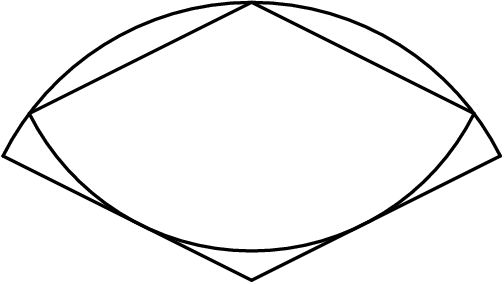
\includegraphics[scale=0.8]{Sections/Files/13-1-4.png}
    \end{center}
    %Put Problem Here
}\bigskip

\begin{solution}\hfil\medskip
	
    Let $r < R$ be the two radii of the sectors. Notice that the two red triangles shown below are both right triangles (one's a tangent, the other's the symmetry axis of an isosceles triangle)
    and one of their acute angles is $\frac{\theta}{2}$ in both triangles; since they share the same hypotenuse the two are congruent. Then by Pythagorean Theorem we have
    $$r^2 + \left(\dfrac{r}{2}\right)^2 = R^2 = \dfrac{5r^2}{4} \iff \dfrac{r}{R} = \dfrac{2}{\sqrt{5}} = \sin\left(\dfrac{\theta}{2}\right)$$
    so by double angle formula we have $$\cos(\theta) = 1 - 2 \sin^2\left(\dfrac{\theta}{2}\right) = -\dfrac{3}{5} \iff \boxed{305}.$$

    \begin{center}
        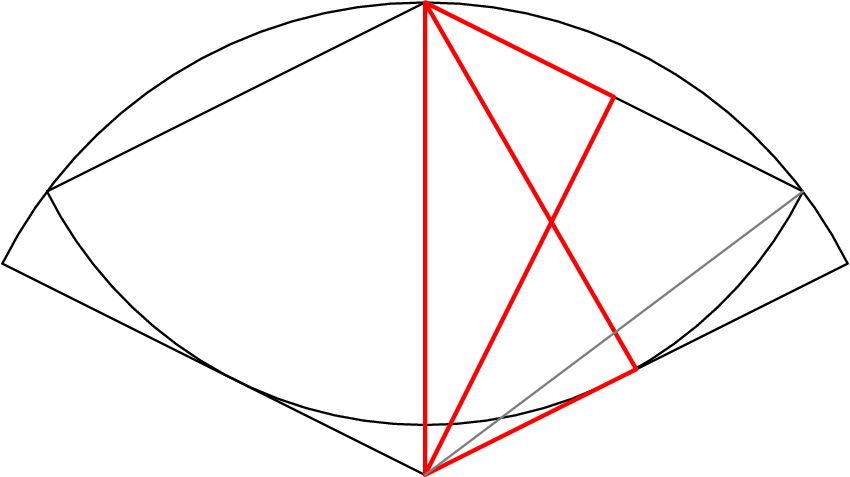
\includegraphics[scale=0.4]{Sections/Files/13-1-4S.png}
    \end{center}
    %Put sol here
\end{solution}\bigskip

	\newpage

    \subsubsection{Graph Theory in Disguise}
	\label{13.1.5}
	
\SSbreak\\
\emph{Source: CMC Mock ARML 2019 P10}\\
\emph{Proposer: \Pnjoy}\\
\emph{Problem ID: 179}\\
\emph{Date: 2021-04-23}\\
\emph{Difficulty: Hard}\\
\SSbreak

\SSpsetQ{
  Tony and Wang play a game in which Tony chooses a list of $6$ real numbers and Wang devises $6$ questions, each of the form ``What is the sum of the $x^{\text{th}}$ and $y^{\text{th}}$ number in your list?'' where $1\leq x<y\leq 6.$ Without regard to order, compute the number of ways Wang can choose his questions so that he can determine Tony's numbers.
}\bigskip

\begin{solution}[Solution by \Pnjoy]\hfil\medskip

    We can consider the the game as a graph with 6 vertices, representing Tony’s numbers, and 6 edges,representing Wang’s questions.  Note that we can’t have a cycle with even length since then the corresponding system of equations wouldn’t be linearly independent.  For example, the system of equations $x+y=c_1$, $y+z=c_2$, $z+w=c_3$, $w+x=c_4$ is not linearly independent, since the sum of the 1\textsuperscript{st} and 3\textsuperscript{rd} equations is equal to the sum of the 2\textsuperscript{nd} and 4\textsuperscript{th}; hence one equation is wasted, yet 6 independent equations are required to find 6 variables. Since the largest tree in a graph with 6 vertices consists of 5 edges, a cycle must exist.  We distinguish three cases, depending on the length of the largest cycle:
    \begin{enumerate}
    \item We have a 5-cycle.  There are 6 ways to choose which number is left out of the 5-cycle, 12 ways to order the elements of the 5-cycle, and 5 ways to connect the number left out to the cycle, for a total of 360 possibilities.
    \item There are two 3-cycles.  As the cycles are disjoint, there are \(\frac{\binom{6}{3}}{2}= 10\) such possibilities.
    \item There is only one 3-cycle.  We choose the cycle $C$ in \(\binom{6}{3}= 20\) ways, and then choose the paths to connect the other three vertices $(X, Y, Z)$to $C$, where each of these points must have exactly 1 path.  If $X \rightarrow C$, $Y \rightarrow C$ and $Z \rightarrow C$,there are $3^3= 27$ ways; if$X \rightarrow Y \rightarrow C$,and$Z \rightarrow C$(and permutations), there are $6 \times 3^2= 54$ ways; if $X \rightarrow Z, Y \rightarrow Z$and \(Z\rightarrow C\)(and permutations), there are \(3\cdot3 = 9\) ways; finally, if \(X\rightarrow Y\rightarrow Z\rightarrow C\) (and permutations), there are \(6\rightarrow3 = 18\) ways, for a total of \(20\rightarrow(27 + 54 + 9 + 18) = 2160\) possibilities.Thus, Wang has a total of \(360 + 10 + 2160 = 2530\)
    \item Case 3: there is only one 3-cycle.  We choose the cycle \(C\in(63)= 20\) ways, and then choose the paths to connect the other three vertices \(X, Y, Z\rightarrow C\),where each of these points must have exactly 1 path. If \(X→C, Y\rightarrow C\) and \(Z\rightarrow C\),there are 33 = 27 ways; if \(X\rightarrow Y\rightarrow C\) and \(Z\Rightarrow C\) (and permutations), there are \(6\cdot32= 54\) ways; if \(X\rightarrow Z, Y\rightarrow Z\) and \(Z\rightarrow C\)(and permutations), there are \(3\cdot3 = 9\) ways; finally, if \(X\rightarrow Y\rightarrow Z\rightarrow C\)(and permutations), there are \(6\cdot3 = 18\) ways, for a total of \(20\cdot(27 + 54 + 9 + 18) = 2160\) possibilities. Thus, Wang has a total of \(360 + 10 + 2160 =2530\)
    \end{enumerate}

\end{solution}\bigskip

	\newpage

    \subsubsection{What the H-E-double hockey sticks?}
	\label{13.1.6}
	\SSbreak\\
\emph{Source: old italian contest}\\
\emph{Proposer: \Pmatt}\\ %\Pchan \Pbrain \Pss
\emph{Problem ID: 180}\\
\emph{Date: 2021-04-24}\\
\emph{Difficulty: Challenging}\\
\SSbreak
 
\SSpsetQ{
    There are $2021$ people working in a $2021$-floor building, one on each floor. On day zero, each worker writes a zero on their sheet of paper. On day $k > 0$,
    the worker on floor $f > 1$ writes on their sheet of paper the sum of the numbers of the worker on floor $j - 1$ had written in the days up to $k - 1$. The worker
    on floor $1$, meanwhile, writes $k^2$. If $N$ is the number the worker on floor $2021$ writes on day $10000$, find the number of digits in $\nu_2(N) + \nu_3(N) + \nu_5(N)$.
    \begin{center}
        \textit{(A scientific calculator may be used.)}
    \end{center}
    %Put Problem Here
}\bigskip

\begin{solution}\hfil\medskip
	
    We denote worker $f$ as the worker who works on floor $f$. It's clear that on day $k$, worker $2$ writes $$1^2 + 2^2 + \cdots + (k - 1)^2 = \dfrac{k(k - 1)(2k - 1)}{6}$$
    using the well-known sum of squares formula, but it's hard to see where it goes from here. Instead, write $k^2$ as a sum of binomial coefficients. We know that $2\binom{k}{2} = k(k - 1) = k^2 - k$
    and $\binom{k}{1} = k$, so we have $$k^2 = 2\dbinom{k}{2} + \dbinom{k}{1} \iff 1^2 + 2^2 + \cdots + (k - 1)^2 = 2\left[\dbinom{2}{2} + \dbinom{3}{2} + \cdots + \dbinom{k - 1}{2}\right] + \left[\dbinom{1}{1} + \dbinom{2}{1} + \cdots + \dbinom{k - 1}{1}\right]$$
    which sums to $2\binom{k}{3} + \binom{k}{2}$ after applying the hockey stick identity. Use the hockey stick identity again and again to show that on day $k$, 
    worker $f$ writes down the number $$2\dbinom{k}{f + 1} + \dbinom{k}{f} = \dbinom{k + 1}{f + 1} + \dbinom{k}{f + 1} = \dbinom{k}{f + 1} \cdot \dfrac{2k - f + 1}{k - f}.$$ Substituting $f = 2021, k = 10000$ (and doing either Legendre or Krummer's) yields \fbox{25}.
    %Put sol here
\end{solution}\bigskip

	\newpage

    \subsubsection{"What's an mgf?"}
	\label{13.1.7}
	\SSbreak\\
\emph{Source: 2013 HMMT C9}\\
\emph{Proposer: \Pchan}\\ %\Pchan \Pbrain \Pss
\emph{Problem ID: 181}\\
\emph{Date: 2021-04-25}\\
\emph{Difficulty: Challenging}\\
\SSbreak
 
\SSpsetQ{
    Given a permutation $\pi$ of $\{1, 2, \cdots , 2021\}$, let $p(\pi)$ be the number of fixed points of $\pi$. If $P$ is the set of all permutations $\pi$,
    then let $$N = \sum_{\pi \in P} p(\pi)^4.$$ Find $\nu_2(N) + \nu_3(N) + \nu_5(N)$.
    \begin{center}
        \textit{(A scientific calculator may be used.)}
    \end{center}
    %Put Problem Here
}\bigskip

\begin{solution}\hfil\medskip
	
    \href{https://hmmt-archive.s3.amazonaws.com/tournaments/2013/feb/comb/solutions.pdf}{Contest Solutions} Answer: \fbox{3523}
    %Put sol here
\end{solution}\bigskip

	\newpage

\ihead{\footnotesize\bfseries\sffamily{Quality Uncontrol (Season 13), Week 2}}
\subsection{Week 2}

    \subsubsection{It's Okay :)}
    \label{13.2.1}
    \SSbreak\\
\emph{Source: Adapted from a FTW problem.}\\
\emph{Proposer: \Pequals}\\ %\Pchan \Pbrain \Pss
\emph{Problem ID: 182}\\
\emph{Date: 2021-04-26}\\
\emph{Difficulty: Beginner}\\
\SSbreak

\SSpsetQ{

A two-digit positive integer, $n$, is doubled and then added to $2$ to obtain $N$. Then, the digits of $n$ are reversed to form a new positive integer $m$. Given that $N=m$, find $n$.
	%Put Problem Here
}\bigskip

\begin{solution}\hfil\medskip
	
	(Sorry, I don't know how to use LaTeX.)

Answer: \fbox{25}

It is not too difficult to find the answer through educated guessing and checking, but below is a solution that does not require guessing.

Let $x$ be the tens digit of $n$ and let $y$ be the ones digit of $n$.

Then the problem can be translated into:
$2(10x+y)+2=10y+x$

Simplifying the equation, we get:
$19x=8y-2$

We can easily deduce that:
$19x=8y-2=38$

Therefore:
$x=2 and y=5$

Finally:
$n=10x+y=25$
	%Put sol here
\end{solution}\bigskip

    \newpage

    \subsubsection{Points on a Line}
	\label{13.2.2}
	\SSbreak\\
\emph{Source: Online Mathematics Open Spring 2020 Problem 1}\\
\emph{Proposer: \Pnjoy}\\ %\Pchan \Pbrain \Pss
\emph{Problem ID: 183}\\
\emph{Date: 2021-04-27}\\
\emph{Difficulty: Beginner}\\
\SSbreak

\SSpsetQ{
	Let $\ell$ be a line and let points $A$, $B$, $C$ lie on $\ell$ so that $AB = 7$ and $BC = 5$. Let $m$ be the line through $A$ perpendicular to $\ell$. Let $P$ lie on $m$. Compute the smallest possible value of $PB + PC$.
	%Put Problem Here
}\bigskip

\begin{solution}\hfil\medskip
	
	Clearly, the minimum occurs when $A = P$. If $C$ is between $A$ and $B$ then the distance $PB + PC$ is lower than if $C$ is not between $A$ and $B$, giving us an answer of \fbox{9}. 
	%Put sol here
\end{solution}\bigskip

	\newpage

    \subsubsection{Diamond Operator}
	\label{13.2.3}
	\SSbreak\\
\emph{Source: PUMaC 2017 A1}\\
\emph{Proposer: \Pchan}\\ %\Pchan \Pbrain \Pss
\emph{Problem ID: 184}\\
\emph{Date: 2021-04-28}\\
\emph{Difficulty: Easy}\\
\SSbreak

\SSpsetQ{
	Let $a \diamond b = ab - 4(a+b) + 20$. Evaluate \[1 \diamond (2 \diamond (3 \diamond (\cdots (2020 \diamond 2021)\cdots )))\]
	%Put Problem Here
}\bigskip

\begin{solution}\hfil\medskip
	
	\href{https://static1.squarespace.com/static/570450471d07c094a39efaed/t/5a1784b6e4966b1342975a24/1511490742989/PUMaC2017_Algebra_A_Solutions.pdf}{Official Solution} Answer: \fbox{4}
	%Put sol here
\end{solution}\bigskip

	\newpage
    
    \subsubsection{Weird Wilson}
	\label{13.2.4}
	\SSbreak\\
\emph{Source: Baltic Way [Unknown]}\\
\emph{Proposer: \Ptroll}\\ %\Pchan \Pbrain \Pss
\emph{Problem ID: 185}\\
\emph{Date: 2021-04-29}\\
\emph{Difficulty: Medium}\\
\SSbreak
 
\SSpsetQ{
    Find the smallest prime factor of $712! + 1$.
    %Put Problem Here
}\bigskip

\begin{solution}\hfil\medskip
	
    Unfortunately, $713$ is not prime; neither is $715$ nor $717$. $719$ is prime, so by Wilson's Theorem we know that $718! \equiv 1 \pmod{719}$. Now we 
    rewrite $718!$ as follows: $$718! = 718 \cdot 717 \cdot 716 \cdot 715 \cdot 714 \cdot 713 \cdot 712! \equiv (-1)(-2)(-3)(-4)(-5)(-6) \cdot 712! \equiv 712! \equiv 1 \pmod{719}$$
    so $\boxed{719} | 712! + 1.$
    %Put sol here
\end{solution}\bigskip

	\newpage

    \subsubsection{Get the CRUX of this inequality!}
	\label{13.2.5}
	\SSbreak\\
\emph{Source: CRUX Mathematicorum}\\
\emph{Proposer: \Pnjoy}\\ %\Pchan \Pbrain \Pss
\emph{Problem ID: 186}\\
\emph{Date: 2021-04-30}\\
\emph{Difficulty: Hard}\\
\SSbreak

\SSpsetQ{

Six positive real numbers $r_1, r_2, r_3, r_4, r_5, r_6$ are such that $$3\cdot\left(\sum_{i=1}^6 (-1)^i r_i\right) = \sum_{i=1}^6 r_i^2 = 18.$$ If $M$ is the least possible constant such that $r_1r_2r_3r_4r_5r_6 \leq M$, find the value of $\lfloor 100M \rfloor$.
}\bigskip

\begin{solution}\hfil\medskip
  
Source: \href{https://cms.math.ca/wp-content/uploads/crux-pdfs/CRUXv44n6.pdf}{\textbf{CRUX Mathematicorum (go to Page 44-45)}} Answer: \fbox{100}
\end{solution}\bigskip

	\newpage

    \subsubsection{Don't overthink this}
	\label{13.2.6}
	\SSbreak\\
\emph{Source: Original (?)}\\
\emph{Proposer: \Pchris}\\ %\Pchan \Pbrain \Pss
\emph{Problem ID: 187}\\
\emph{Date: 2021-05-01}\\
\emph{Difficulty: Challenging}\\
\SSbreak
 
\SSpsetQ{
    Points $A, B, C, D$ are located at $(-3, 0), (1, 0), (6, 0), (7, 0)$ in the coordinate plane. If the locus of points $P$ such that 
    the circumcircles of $\triangle ABP$ and $\triangle CDP$ are tangent has perimeter $p$, find $\lfloor 100p \rfloor$.
    %Put Problem Here
}\bigskip

\begin{solution}\hfil\medskip
	
    Let $X$ have coordinates $(x, y)$, and $Y$ be the intersection of the radical axis of the two circumcircles and segment $\overline{BC}$.
    Let $BY = b$; then $CY = 5 - b$. By Power of a Point, we have $$XY^2 = BY \cdot AY = CY \cdot DY = b(4 + b) = (5 - b)(6 - b) \iff b = 2, XY^2 = 12$$
    so $X$ is always a distance of $\sqrt{12}$ from the point $Y = (3, 0)$; this is a circle with radius $\sqrt{12}$ and so our answer is \fbox{2176}.
    %Put sol here
\end{solution}\bigskip

	\newpage

    \subsubsection{The Party, The Politburo, and the PSC}
	\label{13.2.7}
	\SSbreak\\
\emph{Source: IZhO 2021/5}\\
\emph{Proposer: \Phyper}\\ %\Pchan \Pbrain \Pss
\emph{Problem ID: 188}\\
\emph{Date: 2021-05-02}\\
\emph{Difficulty: Challenging}\\
\SSbreak

\SSpsetQ{
On a party with $102$ guests, hosts Tony and Wang play a game (the hosts are not regarded as guests). There are $102$ chairs arranged in a circle; initially, all guests hang around those chairs. The hosts take turns alternately. By a turn, a host orders any standing guest to sit on an unoccupied chair $c$. If some chair adjacent to $c$ is already occupied, the same host orders one guest on such chair to stand up (if both chairs adjacent to $c$ are occupied, the host chooses exactly one of them). All orders are carried out immediately. Tony makes the first move; her goal is to fulfill, after some move of hers, that at least $k$ chairs are occupied. Determine the largest $k$ for which Tony can reach the goal, regardless of Wang's play.

%Put Problem Here
}\bigskip

\begin{solution}\hfil\medskip
 
We claim the answer is \fbox{35}. Note the number of chairs does not decrease, given that every empty chair must be next to a full chair, we have at least 34 chairs. In addition, when there are 33 chairs, every third chair is occupied.
 
 If Wang forces Tony into such a configuration, say Tony placed a guest on chair $x$ and Wang on $y$. However, if $y$ is adjacent to $x$, Tony could have easily have chosen $y$ instead and wins. Otherwise, she could have placed it on $x\pm 1$, as there were no guests there, and now not every third chair is occupied. Thus, Wang never reaches a position with 34 chairs such that no more guests can be placed for Tony, and Tony can happily place her last guest.
 
 To show that Wang can win otherwise, we show inductively that Wang can hold a strategic position:\\
 \textbf{Claim.} Wang can make sure that in the sets $S_2,S_3,\ldots,S_{34}$ where $S_k=\{3k+1,3k+2,3k+3\}$, none of $3k+1$ and $3k+3$ is occupied. Furthermore, there is at most two occupied chairs in $S_1$.\\
 \textbf{Proof.} The proof is by induction.\\
 \textit{Base Case.} No moves are made, in which case the claim holds.\\
 \textit{Induction Hypothesis.} Assume that Wang holds such a position. We claim after 2 moves, Wang can hold this position again.
 \textit{Induction Step.} If Alice's move holds the position, Wang can simply put a person somewhere in $S_1$ (as chairs 4 and 102 are unoccupied, we can once again only have at most 2 people in $S_1$). If it doesn't, she could not have operated on $S_1$, and thus placed a guest in some of $S_2,\ldots,S_{99}$. However, if she operates on $S_k$, Wang places a person in the middle of $S_k$ and removes the mischief caused by Alice. Thus Wang can hold his position.
%Put sol here
\end{solution}\bigskip

	\newpage

\ihead{\footnotesize\bfseries\sffamily{Mityushikha Bay (Season 14)}}
\section{Mityushikha Bay (Season 14)}

    \ihead{\footnotesize\bfseries\sffamily{Mityushikha Bay (Season 14), Week 1}}
    \subsection{Week 1}

    \subsubsection{Rectangle Rotation}
	\label{14.1.1}
	\SSbreak\\
\emph{Source: Original}\\
\emph{Proposer: \Prandom}\\ %\Pchan \Pbrain \Pss
\emph{Problem ID: 189}\\
\emph{Date: 2021-05-17}\\
\emph{Difficulty: Beginner}\\
\SSbreak

\SSpsetQ{
    A 35-by-42 rectangle is rotated around one of its vertices. If $A$ is the area the rectangle sweeps out, find $\lfloor 100A \rfloor.$

    \begin{center}
        \textit{(A scientific calculator may be used.)}
    \end{center}
    %Put Problem Here
}\bigskip

\begin{solution}\hfil\medskip
	
	Noticably after a rectangle is rotated around one of its vertex, it will then form a circle. \\
The radius of the circle is a diagonal because the furthest point from one of its vertex is a diagonal and in a few rotation, it will cover an area of circle with the radius of the diagonal length. \\
Firstly, calculate the radius of the circle by calculating the rectangle diagonal \\
$ r = \sqrt{a^2 + b^2} $ \\
$ r = \sqrt{35^2 + 42^2} $ \\
$ r = \sqrt{2989} $ \\
so the area of the circle of $2989\pi \iff \boxed{939022}$. \medskip

\textit{Remark.} $3.1415926$ and $\frac{355}{113}$ are the least "precise" approximations of $\pi$ needed to get the correct answer.
	%Put sol here
\end{solution}\bigskip

	\newpage

	\subsubsection{NJOY Troll (again)}
	\label{14.1.2}
	\SSbreak\\
\emph{Source: Original}\\
\emph{Proposer: \Pnjoy}\\ %\Pchan \Pbrain \Pss
\emph{Problem ID: 190}\\
\emph{Date: 2021-05-18}\\
\emph{Difficulty: Beginner}\\
\SSbreak

\SSpsetQ{

If the minimum of $(20 \cos x + 21)^2 + 2021$ is $M$, find $\lfloor 100M \rfloor$.
}\bigskip

\begin{solution}\hfil\medskip
  
    The expression inside the square has a minimum of $1$, achieved when $\cos x = -1.$ Answer: \fbox{202200}
\end{solution}\bigskip

	\newpage

	\subsubsection{You Just Got Vector'ed}
	\label{14.1.3}
	\SSbreak\\
\emph{Source: Sixth Term Examination Paper I, 2013 Q3}\\
\emph{Proposer: \Pss}\\
\emph{Problem ID: 191}\\
\emph{Date: 2021-05-19}\\
\emph{Difficulty: Easy}\\
\SSbreak
 
\SSpsetQ{Given for any two points $X$ and $Y$, with position vectors
$\textbf x$ and $\textbf y$ respectively, $X*Y$ is defined
to be the point $Z$ along the line $\overleftrightarrow{XY}$ such that $$\dfrac{XZ}{ZY} = \dfrac{\lambda}{1 - \lambda},$$
where $\lambda$ is a fixed number. \medskip

The points $P_1$, $P_2$, $\ldots$
are defined by $P_1 = X*Y$ and, for $n \ge2$, $P_n= P_{n-1}*Y\,.$ Given that $X$ and $Y$ are distinct and that $0<\lambda<1$, the ratio in which $P_n$ divides the line segment $XY$ can be expressed in the form \(1:A\). 
If $\lambda = 0.75$ and $n = 69$, find $\left \lfloor 10^{12} A \right \rfloor$.
  
\begin{center}
\textit{(A scientific calculator may be used.)}
\end{center}
}\bigskip

\begin{solution}\hfil\medskip

 We have
\begin{align*}
    P_1&=X*Y\\
    P_2&=(X*Y)*Y\\
    \cdots&\\
    P_n&=(X*Y)*Y)*Y)...*Y
\end{align*}
Where \(P_n\) has \(n\) \(Y\)'s. Substituting \(X*Y=\lambda\textbf{x}+(1-\lambda)\textbf{y}\) and going through a number of iterations of \(*Y\), we guess \(P_n=\lambda^n+(1-\lambda^n)\textbf{y}\).\\

We now proceed by induction on \(n\). Given we have already verified the case of \(n=1\), let \(n=k,\ k\in\N\) and assume \(P_k=\lambda^k\textbf{x}+(1-\lambda^k)\textbf{y}\). Then for \(n=k+1\), we have \(P_{k+1}=P_k*Y\), and so we have \(P_{k+1}=\lambda^{k+1}\textbf{x}+\lambda(1-\lambda^k)\textbf{y}+(1-\lambda)\textbf{y}\). This simplifies to \(P_{k+1}=\lambda^{k+1}\textbf{x}+(1-\lambda^{k+1})\textbf{y}\), as required. Therefore:

\begin{equation*}
    P_n=\begin{pmatrix}
        \lambda^n \\ 1-\lambda^n
    \end{pmatrix}
\end{equation*}
Now it's simply a case of
\begin{equation*}
    XY:P_n=\begin{pmatrix}
        1\\ 1
    \end{pmatrix} : \begin{pmatrix}
        \lambda^n \\ 1-\lambda^n
    \end{pmatrix}\Rightarrow XY:P_n=1:\frac{\lambda^n}{1-\lambda^n}
\end{equation*}
Hence when \(\lambda=0.75\) and \(n=69\), we have \(\{10^{12}\cdot A\}=\fbox 2394\)
\end{solution}
	\newpage

	\subsubsection{Answer Extraction}
	\label{14.1.4}
	\SSbreak\\
\emph{Source: Original}\\
\emph{Proposer: \Ppi}\\ %\Pchan \Pbrain \Pss
\emph{Problem ID: 192}\\
\emph{Date: 2021-05-20}\\
\emph{Difficulty: Medium}\\
\SSbreak

\SSpsetQ{
	On a QoTD, the PSC has a probability $\frac{m}{n}$ that they need to decide how to make people submit. Sjbs thinks that people should submit $m+n$. Brainy however, thinks that the people should submit $100m+n$. The rest of the PSC come up with an even better idea of people submitting $420m+69n$. 

If the PSC decides every single answer will be $420$ in a season, the number of possible ways they can choose $m$ and $n$ and a way of formatting their answer ( $420m+69n$, $100m+n$, or $m+n$ ) in a $14$ day season can be written as $a^b$ where $a$ and $b$ are positive integers and $b$ is maximized. Compute $420a+69b$.

(The PSC can use a specific $\frac{m}{n}$ more than once.)
	%Put Problem Here
}\bigskip

\begin{solution}\hfil\medskip
	
    We can do some casework.

Case $1$: The PSC choose to use the $420m+69n = 420$ system
Clearly only $m=1, n=0$ works, however this will not fit into the constraints. \medskip

Case $2$: The PSC choose to use the $100m+n = 420$ system
Only $(0,420), (1,320), (2,220), (3,120), (4,20)$ work, and of these, only $(1, 320)$ works. \medskip

Case $3$: The PSC choose to use the $m+n=420$ system. 
For this to work we must have $\gcd(m, n) = \gcd(m, 420-m) = \gcd(m, 420) = 1$. So to calculate the number of $m$ possible, we do $\phi(420) = 420 \cdot \frac{1}{2} \frac{2}{3} \frac{4}{5} \frac{6}{7} = 96$. Since $m$ must also be greater than $n$ we divide by $2$ to get $48$ ways. \medskip

So our answer is $49^{14} = 7^{28} \iff \boxed{4872}.$
	%Put sol here
\end{solution}\bigskip

	\newpage

    \subsubsection{Not a Fan}
	\label{14.1.5}
	\SSbreak\\
\emph{Source: Baltic Way 2020 Problem 18}\\
\emph{Proposer: \Phyper}\\ %\Pchan \Pbrain \Pss
\emph{Problem ID: 193}\\
\emph{Date: 2021-05-21}\\
\emph{Difficulty: Hard}\\
\SSbreak

\SSpsetQ{

Let $n\geq 1$ be a positive integer. We say that an integer $k$ is a \emph{fan} of $n$ if $0\leq k\leq n-1$ and there exist integers $x,y,z\in\mathbb{Z}$ such that
\begin{align*}
	x^2+y^2+z^2 &\equiv 0 \pmod n;\\
	xyz &\equiv k \pmod n.
\end{align*}Let $f(n)$ be the number of fans of $n$. Determine $f(2020)$.
%Put Problem Here
}\bigskip

\begin{solution}\hfil\medskip

We note that if $4\mid x^2+y^2+z^2$, then clearly $x\equiv y\equiv z\equiv 0\pmod 2$, so $xyz\equiv 0\pmod 4$. Similarly, if $5\mid x^2+y^2+z^2$, then as $x^2\in\{0,1,4\}$, one of $x,y,z$ is divisible by $5$. Now, we claim we can find $x,y,z$ such that $x^2+y^2+z^2\equiv 0\pmod{101}$ and $xyz\not\equiv 0\pmod{101}$. We can let $\alpha=\sqrt{-1}\pmod{101}$ which has to exist as $101\equiv 1\pmod 4$. Thus if $101\nmid z$,
\[(x-\alpha y)(x+\alpha y)=x^2-(\alpha y)^2=-z^2\]
We have $101-1=100$ choices for $x+\alpha y$, and only two values of $x+\alpha y$ force $x+\alpha y=\pm (x-\alpha y)$, implying that we have a solution such that $0\nmid x,y,z$ and
\[101\mid x^2+y^2+z^2\]
Note that $3\nmid 101-1$, so thus taking this solution and multiplying by an arbitrary number $w$, we see that $(xw,yw,zw)$ works and thus spans all possible values of $k\pmod{101}$. Thus, there are 101 \emph{fans} of 101, but only 1 of \emph{20}, so there are \boxed{101} of 2020.
%Put sol here
\end{solution}\bigskip

	\newpage

	\subsubsection{you're welcome, brainy}
	\label{14.1.6}
	\SSbreak\\
\emph{Source: 2019 Turkey Math Olympiad, P3}\\
\emph{Proposer: \Palp}\\ %\Pchan \Pbrain \Pss
\emph{Problem ID: 194}\\
\emph{Date: 2021-05-22}\\
\emph{Difficulty: Challenging}\\
\SSbreak
 
\SSpsetQ{
    There are 2021 crewmates in the universe, and some of these crewmates are members of different crews (crewmates can belong to multiple crews at once). 
    Each crew has a security council consisting of 12 crewmates who are members of that particular crew. 
    An \textit{emergency meeting} (for a particular crew) can be realized only when each participant (of the meeting) is a member of that crew, and moreover, 
    each of the 12 crewmates forming the security council (for that crew) are present among the participants. 
    It is known that each subset of at least 12 crewmates can realize an emergency meeting for exactly one crew. 
    If the total number of different crews with exactly 29 crewmates is $N$, find $\nu_2(N) + \nu_3(N) + \nu_5(N).$
    %Put Problem Here
}\bigskip

\begin{solution}\hfil\medskip
	
\href{https://artofproblemsolving.com/community/c6h1974664p13698434}{AoPS Solutions} \medskip

The answer is $\binom{2003}{11} \iff \boxed{4}.$
    %Put sol here
\end{solution}\bigskip

	\newpage

	\subsubsection{RDS-1}
	\label{14.1.7}
	\SSbreak\\
\emph{Source: 2007 Sharygin Correspondence Round 18}\\
\emph{Proposer: \Paiya}\\ %\Pchan \Pbrain \Pss
\emph{Problem ID: 195}\\
\emph{Date: 2021-05-23}\\
\emph{Difficulty: Challenging}\\
\SSbreak
 
\SSpsetQ{
    $O, G$ are points in the plane such that $OG = 20.21$. Let $S$ be the set of vertices of all triangles with positive area that have circumcentre $O$ and centre of mass $G$,
and $T$ the set of points in the plane that are not in $S$. If the area of $T$ is $U$, find $\lfloor 100U \rfloor$.
    \begin{center}
        \textit{(A scientific calculator may be used.)}
    \end{center}
    %Put Problem Here
}\bigskip

\begin{solution}\hfil\medskip
	
    The \href{https://geometry.ru/olimp/2007/zaochsol.pdf}{official solution} is in Russian. I don't understand Russian. \medskip

    The main motivation here is the Euler Line and the points on it. 

    \textit{Euler Line.} $O, G, H$, circumcentre, centre of mass, and orthocentre of a triangle, are collinear with $2OG = GH$ or all three coincident. 
    Consider the homothety that sends each vertex of $\triangle ABC$ to the midpoint of its opposite side, thus sending $\triangle ABC$ to its 
    medial triangle; this homothety is then centered at $G$ (why?). Then, $H$ is mapped to the orthocentre of the medial triangle, but this point is
    the circumcentre of $\triangle ABC$. \medskip

    \textit{Lemma.} Let $F$ be the midpoint of $\overline{AB}$. Then, $CH = 2OF$. This is closely related with the proof of the existence of the nine-point-circle.
    Consider the homothety centered at $N_9$ that sends $O$ to $H$; this homothety has scale $-1$. Then, $F$ is sent to the midpoint of $\overline{CH}$ since the foot
    of the $C$-altitude is on the nine-point-circle, implying that $F$ and the midpoint of $\overline{CH}$ are diametrically opposite. We are done. \medskip

    But note that $OF < R$, so we have the constraint $CH = 2OF < 2R = 2OC$. The locus for which $\frac{CH}{OC} \leq 2$ is a union of Apollonian circles forming 
    a disk with the boundary circle being the Apollonian circle where $\frac{CH}{OC} = 2$. Two diametrically opposite points on this circle are $G$ and $G'$, where
    $G'$ is on the Euler line and $G'O = 60.63$, making the disk have radius $40.42$. To construct such $\triangle ABC$, let $F$ be the point on $\overrightarrow{CG}$ such that
    $CF > CG$ and $CG = 2GF.$ Then draw a line at $F$ perpendicular to $\overline{OF}$ and a circle centered at $O$ with radius $OC$; the points $A, B$ are the 
    intersections of circle and line. \medskip

    \begin{center}
        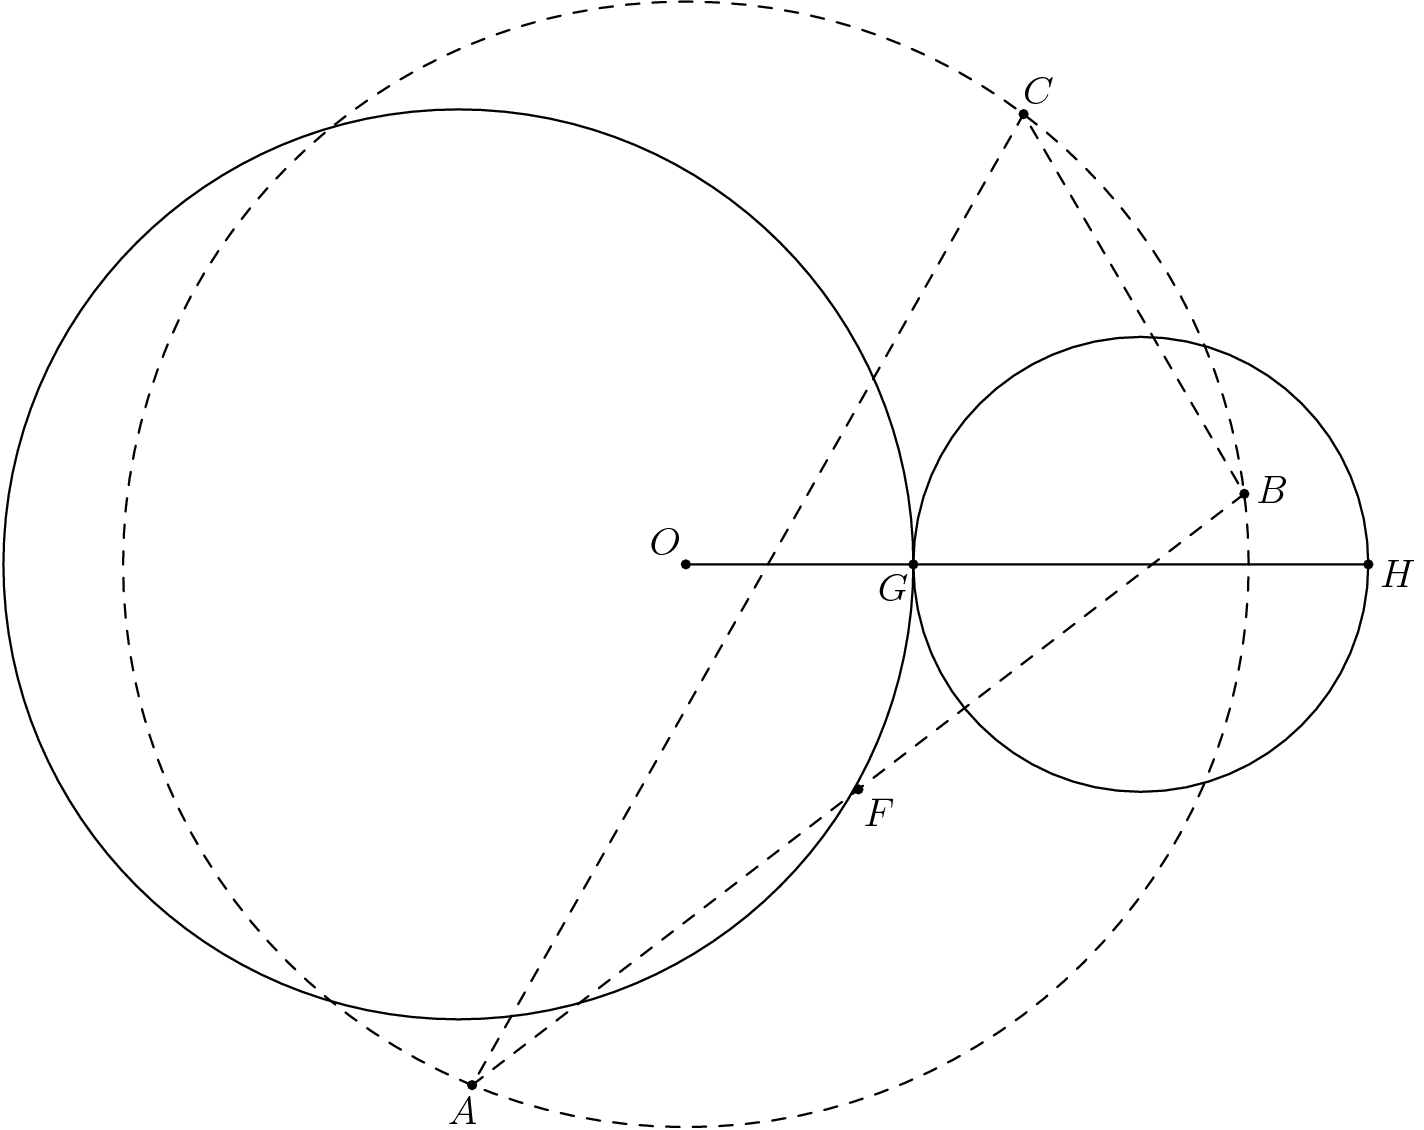
\includegraphics[scale=0.4]{Sections/Files/14-1-7.png}
    \end{center}

    We are missing one detail: what if $A, B, C$ are all collinear? Then, since $\overline{FO} \parallel \overline{CH}$ we have $\angle CFO = \angle GCH$, 
    but since $A, B, C$ collinear we have $\angle CFO = 90$, or, $C$ is on the circle with diameter $\overline{GH}$, which in our case has radius $20.21$
    and does not intersect the aforementioned disk. \medskip
    
    Our answer is $100\pi\left(40.42^2 + 20.21^2\right) \iff \boxed{641582}.$ \medskip

    \textit{Remark.} RDS-1 was the first Soviet nuke. 
    %Put sol here
\end{solution}\bigskip

	\newpage
	
	\ihead{\footnotesize\bfseries\sffamily{Mityushikha Bay (Season 14), Week 2}}
    \subsection{Week 2}
	
	\subsubsection{All About that Base}
	\label{14.2.1}
	\SSbreak\\
\emph{Source: Komal C1336}\\
\emph{Proposer: \Pflame}\\ %\Pchan \Pbrain \Pss
\emph{Problem ID: 196}\\
\emph{Date: 2021-05-24}\\
\emph{Difficulty: Beginner}\\
\SSbreak

\SSpsetQ{

    Let $a$, $b$, and $c$ denote the digits $0$, $1$, and $2$, in some order. If \[aaa_3 \times bb_3 = acbab_3,\] evaluate $bcba_{10} \times bcbb_{10}$.

	\begin{center}
		\textit{(A 4-function calculator may be used.)}
	\end{center}
}\bigskip

\begin{solution}\hfil\medskip
  
    If $a$ or $b$ are $0$, then $aaa_3 \times bb_3 = 0_3$, which is clearly false. Hence $c=0$. Looking at the units digits, $a_3 \times b_3 = b_3$, so $a=1$ and $b=2$. (It can be checked that $111_3 \times 22_3 = 10212_3$.) We seek $2021 \times 2022 = \boxed{4086462}$.
\end{solution}\bigskip

	\newpage

	\subsubsection{Number of QoTD Seasons}
	\label{14.2.2}
	\SSbreak\\
\emph{Source: Original}\\
\emph{Proposer: \Pcooked}\\ %\Pchan \Pbrain \Pss
\emph{Problem ID: 197}\\
\emph{Date: 2021-05-25}\\
\emph{Difficulty: Beginner}\\
\SSbreak

\SSpsetQ{
	A QoTD season, lasting 14 days, has 3 alg, 3 combi, 3 geo and 3 NT problems, as well as 2 other problems in any of alg, combi, geo or NT, If $N$ is the number of distinct possible QoTD topic sequences, find $\nu_2(N) + \nu_3(N) + \nu_5(N).$ (Each question belongs to exactly one subject, so no CG or anything.)
	%Put Problem Here
}\bigskip

\begin{solution}\hfil\medskip
	
	Without loss of generality, we can consider two cases- the case that both problems are the same topic and the case that both problems are in different topics.

Consider the case the 2 problems are in the same topic. Without loss of generality, let us call the 4 topics A, B, C and D, and let us assume the 2 problems are in topic A, so that there are 5 A problems, 3 B problems, 3 C problems and 3 D problems. Now, since this is permutations of like objects, we can see the number of topic sequences using A, B, C and D is $$\frac{14!}{5! \times 3! \times 3! \times 3!}$$, which is 3363360. We can also see that there are 4! ways to map Alg, Combi, Geo and NT to the topics A, B, C and D, so there are actually 3363360 $$\times$$ 4! topic sequences, which is 80720640.

Now consider the case the two problems are in different topics. Without loss of generality, let us call the 4 topics A, B, C and D, and let us assume the two problems are in topic A and B respectively, so that there are 4 A problems, 4 B problems, 3 C problems and 3 D problems. Like before, we can see the number of topic sequences using A, B, C and D is $$\frac{14!}{4! \times 4! \times 3! \times 3!}$$ is 4204200. Like before, there are 4! ways to map Alg, Combi, Geo and NT to the topics A, B, C, and D, so there are actually 4204200 $$\times$$ 4! topic sequences, which is 100900800.

Add to get $$\dfrac{14! \cdot 4!}{3!^3 \cdot 4!} \left(\dfrac{1}{5} + \dfrac{1}{4}\right) = 2^6 \cdot 3^4 \cdot \cdot 5 \cdot 7^2 \cdot 11 \cdot 13 \iff \boxed{11}.$$
	%Put sol here
\end{solution}\bigskip

	\newpage

	\subsubsection{Square and Point}
	\label{14.2.3}
	\SSbreak\\
\emph{Source: Original}\\
\emph{Proposer: \Prandom}\\ %\Pchan \Pbrain \Pss
\emph{Problem ID: 198}\\
\emph{Date: 2021-05-26}\\
\emph{Difficulty: Beginner}\\
\SSbreak

\SSpsetQ{
There exist a square $ ABCD $ with its side length 5 and there also exist a random point $ P $ on the same plane such that $ AP = 1 $ . \\
Let $ M $ be the longest distance possible between P and C . Let $ m $ be the shortest distance possible between P and C. \\
Find $\lfloor 1000M + 1000m \rfloor.$

\begin{center}
    \textit{(A scientific calculator may be used.)}
\end{center}
%Put Problem Here
}\bigskip

\begin{solution}\hfil\medskip

We notice that the distance $ CP $ could be maximum and minimum if $ C , A , $ and $ P $ are collinear. This can be proved by drawing a circle around A. Then , we continue by finding M and m \\
M = $ \sqrt{5^2 + 5^2} + 1 $ = $ 5 \sqrt{2} + 1 $ \\
m = $ \sqrt{5^2 + 5^2} - 1 $ = $ 5 \sqrt{2} - 1 $ \\
Hence, $ M + m $ = $ 5 \sqrt{2} + 1 $ + $ 5 \sqrt{2} - 1 $ = $ 10 \sqrt{2} $ = $ \sqrt{200}  \iff \boxed{14142}.$ \\
%Put sol here
\end{solution}\bigskip

	\newpage

	\subsubsection{2012 HMMT A6}
	\label{14.2.4}
	\SSbreak\\
\emph{Source: \Chmmt 2012 February A6}\\
\emph{Proposer: \Pchan}\\
\emph{Problem ID: 199}\\
\emph{Date: 2021-05-27}\\
\emph{Difficulty: Medium}
\SSbreak
 
\SSpsetQ{Let $a_0 = -2$, $b_0 = 1$, and for $n \geq 0$, let 
\[
a_{n+1} = a_n + b_n + \sqrt{a_n^2 + b_n^2}
\]
\[
b_{n+1} = a_n + b_n - \sqrt{a_n^2+b_n^2}
\]

If $a_{2020}$ can be represented in the form $a^x\sqrt{b}- c^y$, where $a,b,c$ are integers such that $a,c$ are minimized and $c$ is square free. Find $x+y$.
}

\begin{solution}\hfil\medskip
By adding the two equations and multiplying them respectively, we get 
\[
a_{n+1} + b_{n+1} = 2(a_n+b_n)
\]
\[
a_{n+1}b_{n+1} = (a_n+b_n)^2 - (a_n^2 + b_n^2) = 2 a_nb_n
\]
Thus, we get that 
\[
a_{2020} + b_{2020} = -2^{2020}
\]
\[
a_{2020}b_{2020} = -2^{2021}
\]
Either by vieta's or substitution, we get $a_{2020}, b_{2020}$ are the roots of  the quadratic
\[
x^2 +2^{2020}x - 2^{2021}
\]
where $a_{2020}$ is the larger root since the positive sqrt was added. Solving the quadratic gives that 
\[
a_{2020} = 2^{1010}\sqrt{2^{2018} + 2} - 2^{2019}
\]
Thus, the answer is $\boxed{3029}$
\end{solution}

	\newpage

	\subsubsection{[under construction]}
	\label{14.2.5}
	% \SSbreak\\
\emph{Source: Probably Not Original}\\
\emph{Proposer: \Paiya}\\ %\Pchan \Pbrain \Pss
\emph{Problem ID: 200}\\
\emph{Date: 2021-05-28}\\
\emph{Difficulty: Hard}\\
\SSbreak

\SSpsetQ{
Let $S$ denote the set $\{0, 1, \cdots , 2026\}^2 \setminus {(0, 0)}$; that is, the set of all pairs of residues mod $2027$ excluding $(0, 0)$.
Let $R(x)$ be the remainder when $$\prod_{(a, b) \in S} (ax + b)$$ is divided by $x^{11} - 1$. Find the remainder when $R(2)$ is divided by $2027$.
}\bigskip

\begin{solution}\hfil\medskip

We solve for general primes, replacing $2027$ with $p$ and $11$ with $q$ such that $q | p - 3$. 
We claim $$x(x + 1)(x + 2) \cdots (x + p - 1) \equiv x^p - x \pmod{p}.$$ 
Indeed, both sides have degree $p$ and roots $0, 1, \cdots p - 1$ mod $p$, so they are equivalent.
When $a = 0$, the product is $(p - 1)!$; we focus on evaluating $ax(ax + 1) \cdots (ax + p - 1)$. 
Note that since $(a, p) = 1$, $\left\{a, 2a, \cdots (p - 1)a\right\}$ is a permutation of $\{1, 2, \cdots p - 1\}$ so our product reduces down to
$$ax(ax + a)(ax + 2a) \cdots \left(ax + (p - 1)a\right) = a^px(x + 1) \cdots (x + p - 1) \equiv a\left(x^p - x\right);$$ multiplying over all $a$ we get
$(p - 1)!^2\left(x^p - x\right)^{p - 1}$. Now, we have $q | p - 3 \iff x^{p - 3} \equiv 1 \pmod{x^q - 1}$ so reducing our product mod $x^q - 1$ yields
$$\left(x^3 - x\right)^{p - 1} \equiv x^{p - 1}\left(x^2 - 1\right)^{p - 1} \equiv x^2\left(x^2 - 1\right)^{p - 1}$$ where we have used $(p - 1)! \equiv -1 \pmod{p}$.
Notice $(-1)^k\binom{p - 1}{k} \equiv (-1)^k \cdot \frac{(-1)(-2) \cdots (-k)}{k!} \equiv 1 \pmod{p}$ so using binomial expansion our product is 
$x^2 + x^4 + \cdots + x^{2p}$. Observe that the $q$ numbers $2, 4, \cdots 2q$ forms a complete residue class mod $q$; this means that 
$$x^2 + x^4 + \cdots x^{2q} \equiv 1 + x + \cdots x^{q - 1} \pmod{x^q - 1}.$$
Letting $p = qk + 3$ we have $p$ terms to sum, so there are $k$ copies of $1 + \cdots + x^{q - 1}$ to sum and an extra $x^2 + x^4 + x^6$ left over. 
Plugging in $x = 2, p = 2027, q = 11, k = 184$ our sum is $$184 \left(2^{11} - 1\right) + 84 \equiv 184 \cdot 20 + 84 \equiv \boxed{1737} \pmod{2027}.$$
\end{solution}\bigskip

	\newpage

	\subsubsection{Projective Pain}
	\label{14.2.6}
	\SSbreak\\
\emph{Source: Unknown}\\
\emph{Proposer: \Pchris}\\ %\Pchan \Pbrain \Pss
\emph{Problem ID: 201}\\
\emph{Date: 2021-05-22}\\
\emph{Difficulty: Challenging}\\
\SSbreak
 
\SSpsetQ{
    $\triangle ABC$ has circumcircle $\Gamma$ and incentre $I$, with sidelengths $AB = 44, BC = 37, CA = 15$. Let $L$ be the midpoint of the arc $\widehat{BC}$ containing $A$. 
    $\overleftrightarrow{LI}$ meets $\Gamma$ again at $D$, and the tangent to $\Gamma$ at $A$ meets $\overleftrightarrow{BC}$ at $P$.
    $\overleftrightarrow{PD}$ meets $\Gamma$ again at $X$. If $Y$ is the point on $\overline{BC}$ such that $\angle BAX = \angle CAY$,
    the ratio $\frac{BY}{CY}$ can be expressed in the form $\frac{m}{n},$ where $m, n$ are relatively prime positive integers. Find $100m + n$.
    %Put Problem Here
}\bigskip

\begin{solution}\hfil\medskip

    \begin{center}
        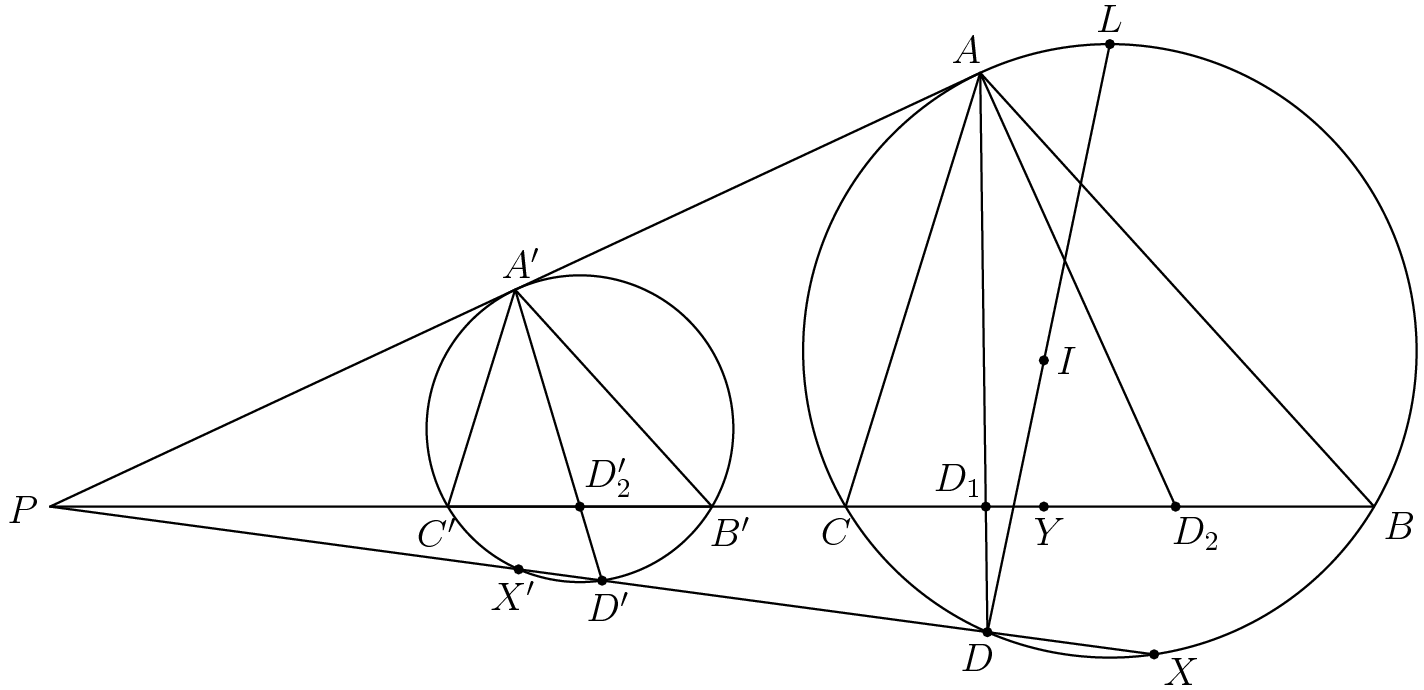
\includegraphics[scale=0.4]{Sections/Files/14-2-6.png}
    \end{center}
	
    We claim that for a general cevian $\ell$ through $A$, $Y$ will be the reflection across the midpoint $M$ of $\overline{BC}$ of the intersection of the isogonal
    line of $\ell$ and $\overline{BC}$. Consider the following transformation that sends points on $\overline{BC}$ to points on $\overline{BC}$: take the projections of points
    wrt $A$ onto $\Gamma$, invert $\triangle ABC$ and those points wrt $P$, project points back onto $\overline{BC}$ wrt $A$, then invert the points back onto the original $\triangle ABC$.
    Let $\overline{AD}$ intersect $\overline{BC}$ at $D_1$, and let $D_2$ be the intersection of the isogonal line of $\overline{AD}$ and $\overline{BC}$. Applying
    this transformation to $\overline{AD}$ and $\overline{AX}$, we let $D', X', B', C', D_2'$ be the images of $D, X, B, C, D_2$ under inversion, and $Y'$ the intersection of $\overline{AD'}$
    and $\overline{B'C'}$; by angle chase we have $\overline{AX'}$ isogonal to $\overline{AD}$ and $\overline{AD'}$ isogonal to $\overline{AX}$. 
    By inversion distance formula we find $$\frac{BY}{CY} = \frac{CD_2}{BD_2} = \frac{PB}{PC};$$ furthermore since $\overline{PA}$ is a tangent 
    we have $\overline{A'C'} \parallel \overline{AB}, \overline{A'B'} \parallel \overline{AC}$ and $\overline{AD'} \parallel \overline{AX}, \overline{AX'} \parallel \overline{AD}$
    so by similar triangles and inversion distance formula we have $$\dfrac{C'D_2'}{A'D_2'} = \dfrac{BD_1}{AD_1}, \dfrac{B'D_2'}{A'D_2'} = \dfrac{CD_1}{AD_1} \iff \dfrac{C'D_2'}{B'D_2'} = \dfrac{PB}{PC} = \dfrac{BD_1}{AD_1} = \dfrac{CD_2}{BD_2}$$
    and we are done. \medskip

    In the case of this problem, it is well-known (in EGMO; invert at A) that $D$ is the touchpoint of the $A$-mixtilinear incircle and $\Gamma$, and so the isogonal line pases through
    the $A$-excircle touchpoint, so $Y$ is actually the incircle touchpoint on $\overline{BC}$ so our answer is $\frac{s - b}{s - c} = \frac{33}{4} \iff \boxed{3304}.$
    %Put sol here
\end{solution}\bigskip

	\newpage

	\subsubsection{AN602}
	\label{14.2.7}
	\SSbreak\\
\emph{Source: 2021 Bundeswettbewerb Mathematik R1P4, Modified}\\
\emph{Proposer: \Pmano}\\ %\Pchan \Pbrain \Pss
\emph{Problem ID: 202}\\
\emph{Date: 2021-05-23}\\
\emph{Difficulty: Challenging}\\
\SSbreak

\SSpsetQ{

    Consider a pyramid with a regular $n$-gon as a base. Draw a line segment in either blue or red between any two points among the n vertices of the base and the apex, except for the edges of the base, which are not drawn at all. Find the smallest integer $n$ with the following property: There exist 4 points among the aforementioned $n+1$ points such that all six segments connecting those four points are drawn in the same color.
}\bigskip

\begin{solution}\hfil\medskip
  
    The solution is $n=\boxed{33}$.
    We first show that $n=32$ does not work, i. e. that we can draw the pyramid with a 32-gon as a base such that there is no complete quadrilateral in a single color. By $R(4,4)=18$, there exists a complete graph $G$ with 17 vertices, the edges drawn in red and blue that contains no $K_4$ (the complete graph with four vertices) drawn in only one color. Now, organise the 32 vertices of the base into pairs, each pair consisting of two neighboring vertices. We have 17 \emph{units} now, 16 pairs of neighboring base vertices and one apex. Now, match every unit with one vertex of $G$ and connect two units in the color in which the edge connecting the correcpoding vertices of $G$ is drawn. Connect two vertices of the pyramid in the color in which the units they are in are connected. As there are no edges drawn within units (because those are neighboring vertices of the base), our construction will indeed work.
    Now show that for $n=33$, there indeed is a $K_4$ as a subgraph drawn in a single color. So consider the pyramid with the regular 33-gon as a base. WLOG, 17 vertices are connected with the apex in red. But among those 17 vertices, there are 9 from which any two are connected. But $R(4,3)=9$, so those 9 vertices contain either a red $K_3$ or a blue $K_4$, where in the first case the pyramid contains a red $K_4$, as desired. \medskip

    This problem is almost impossible without the knowledge of Ramsey numbers, but it can be done; the theory required to discover isn't all that much and 
    you can always search up $R(3, 4)$ and $R(4, 4)$. \medskip

    \textit{2-colour Ramsey numbers.} $R(b, w)$ is the smallest positive integer $n$ such that any edge colouring in black and white of the complete graph on $n$ vertices
    $K_n$ will always contain either an induced subgraph $K_b$ of all black edges or an induced subgraph $K_w$ of all white edges. For example, $R(3, 3) = 6$. 
    To see this, fix one vertex $v$; by pigeonhole at least three of its edges will be of one color, WLOG black. Let the other vertices of those black edges
    be $x, y, z$ respectively. If none of the edges formed by connecting any of $x, y, z$ together are black, then $x, y, z$ is $K_3$; if any of them are then $v$
    and those two vertices forming the other black edge is $K_3$. To prove $R(3, 3) \neq 5$ we can construct a counterexample: take $K_5$ as a pentagon; the perimeter
    of the pentagon is coloured black while all the interior diagonals are coloured white. Convince yourself that this works. \medskip

    \textit{Ramsey's Theorem.} $R(b, w) \leq R(b, w - 1) + R(b - 1, w).$ We proceed by induction on $b + w$. First, convince yourself that $R(b, 2) = b$; 
    this is our base case. Now consider the complete graph on $R(b, w - 1) + R(b - 1, w)$ vertices with edges coloured in black or white. Fix one vertex $v$, and let $B$ be the set of all vertices whose
    edges with $v$ are black, and $W$ the set of all vertices whose edges with $b$ are white. Since $R(b, w - 1) + R(b - 1, w) = |B| + |W| + 1$ we have either
    $|B| \geq R(b - 1, w)$ or $|W| \geq R(b, w - 1)$; WLOG the first case is true. If we have $K_w$ with edges all white we're done; otherwise we have $K_{b - 1}$
    with edges all black; the add in vertex $v$ and all the black edges connected to $v$, which are all from $B$; thus we have $K_b$ all black edges and we're done. 
    If both $R(b, w - 1)$ and $R(b - 1, w)$ are even, the inequality strengthens to $R(b, w) < R(b, w - 1) + R(b - 1, w)$. Consider the complete graph on
    $R(b, w - 1) + R(b - 1, w) - 1$ vertices with edges coloured in black or white. Order the vertices, and let $b_i$ be the \textit{black-degree} of vertex $v_i$; 
    that is, the number of black edges emananting from $v_i$. By handshaking lemma there are an even number of vertices with odd degree; since $R(b, w - 1) + R(b - 1, w) - 1$
    is odd there must exist at least one vertex with even degree; WLOG it's $v_1$. Then $|B| = b_i, |W| = R(b, w - 1) + R(b - 1, w) - 2 - b_i$ are both even, so
    by parity it is impossible for both $|B| < R(b - 1, w) - 1$ and $|W| < R(b, w - 1)$ and we are done.

    \textit{R(3, 4) is 9.} Since $R(3, 3) = 6$ and $R(2, 4) = 4$ are both even we conclude $R(3, 4) < 10$. We can colour a regularly octoganal $K_8$ as follows:
    all perimeter edges are black, and all edges connecting diametrically opposite vertices (vertices 4 apart from another) are black; everything else is white.
    This way, the only way to get from vertex to vertex along black edges is by moving along by $1$ or $4$ vertices; no combination of three ones and fours will be 
    zero mod 8, so there is no black $K_3$; similarly, the only way to get from vertex to vertex along white edges is by moving along by $2$ or $3$ vertices, and the 
    only 4-tuplet of twos and threes that is zero mod 8 are $(2, 2, 2, 2)$ which clearly doesn't work since edges joining antipodeal vertices are coloured black. \medskip

    \textit{R(4, 4) is 18.} We know that $R(4, 4) \leq 2R(3, 4) = 18$. We can colour a regularly 17-gonal $K_{17}$ as follows:
    all edges that connect vertices that are a power of two apart are black and everything else is white. The only combination of $\{1, 2, 4, 8\}$ that is zero mod 17
    is $(8, 4, 4, 1)$ and that doesn't work because a pair of vertices are a distance of twelve apart, and that edge would be coloured white.
    Similarly, the only combination of $\{3, 5, 6, 7\}$ that is zero mod 17 is $(3, 3, 5, 6)$ and that doesn't work be a pair of vertices are a distance 
    of eight apart, and that edge would be coloured black. \medskip

    \textit{Remark.} Mityushikha Bay was the testing site for AN602 (nicknamed the Tsar Bomba), along with many other Russian nukes. 
\end{solution}\bigskip

	\newpage

\ihead{\footnotesize\bfseries\sffamily{SALT-1 (Season 15)}}
\section{SALT-1 (Season 15)}

    \ihead{\footnotesize\bfseries\sffamily{SALT-1 (Season 15), Week 1}}
    \subsection{Week 1}

    \subsubsection{"What are distinct integers?"}
	\label{15.1.1}
	\SSbreak\\
\emph{Source: 2018 Fall OMO 1}\\
\emph{Proposer: \Pnjoy}\\ %\Pchan \Pbrain \Pss
\emph{Problem ID: 204}\\
\emph{Date: 2021-06-07}\\
\emph{Difficulty: Beginner}\\
\SSbreak

\SSpsetQ{

Call two integers \textit{primely} if $1$ is the greatest integer dividing both of them. Find the minimum possible sum of $2021$ nonnegative, primely integers.
}\bigskip

\begin{solution}\hfil\medskip
  
    One zero and $2020$ ones. Answer: \fbox{2020}
\end{solution}\bigskip

	\newpage

	\subsubsection{Troll Pigeonhole}
	\label{15.1.2}
	\SSbreak\\
\emph{Source: \Cop}\\
\emph{Proposer: \Pada}\\ %\Pchan \Pbrain \Pss
\emph{Problem ID: 205}\\
\emph{Date: 2021-06-08}\\
\emph{Difficulty: Beginner}\\
\SSbreak

\SSpsetQ{

	In the following fraction every letter represents a different decimal digit. 
	
	$$\frac{B \cdot L \cdot U \cdot E \cdot B \cdot E \cdot R \cdot R \cdot Y}{I \cdot C \cdot E \cdot C \cdot R \cdot E \cdot A \cdot M}$$
	
	If the sum of all possible real values this expression can take is $S$, find $\floor{100S}$.
}\bigskip

\begin{solution}\hfil\medskip
  
    There are exactly 10 different letters (A, B, C, E, I, L, M, R, U, Y), so one of the letters must be 0. 0 divided by anything (except 0 which will make it undefined) is 0 so the answer is \fbox{0}.
\end{solution}\bigskip

	\newpage

    \subsubsection{WA Can't Solve This}
	\label{15.1.3}
	\SSbreak\\
\emph{Source: 2019 Pui Ching Contest}\\
\emph{Proposer: \Pqs}\\ %\Pchan \Pbrain \Pss
\emph{Problem ID: 206}\\
\emph{Date: 2021-06-09}\\
\emph{Difficulty: Easy}\\
\SSbreak

\SSpsetQ{

    $$\frac{69}{420} + \frac{69\cdot 70}{420\cdot 421} + \frac{69\cdot 70\cdot 71}{420\cdot 421\cdot 422} + \cdots = \frac{m}{n},$$ where $m, n$ are relatively prime
    positive integers. Find $100m + n$.
}\bigskip

\begin{solution}\hfil\medskip
  
    \begin{align} \begin{split}
        &\frac{69}{420} + \frac{69\cdot 70}{420\cdot 421} + \frac{69\cdot 70\cdot 71}{420\cdot 421\cdot 422} + ... \\
        =& \frac{1}{350} \left[ \frac{69\cdot (420-70)}{420} + \frac{69\cdot 70\cdot (421-71)}{420\cdot 421} \right. \\
        &+ \left. \frac{69\cdot 70\cdot 71\cdot (422-72)}{420\cdot 421\cdot 422} + ... \right] \\
        =& \frac{1}{350} \left[ \frac{69\cdot 420}{420} - \frac{69\cdot 70}{420} + \frac{69\cdot 70\cdot 421}{420\cdot 421} - \frac{69\cdot 70\cdot 71}{420\cdot 421} \right. \\
        &+ \left. \frac{69\cdot 70\cdot 71\cdot 422}{420\cdot 421\cdot 422} - \frac{69\cdot 70\cdot 71\cdot 72}{420\cdot 421\cdot 422} + ... \right] \\
        =& \frac{69}{350}
    \end{split} \end{align}
        Thus, the answer is \fbox{7250}.
\end{solution}\bigskip

	\newpage

    \subsubsection{Prime Product}
	\label{15.1.4}
	\SSbreak\\
\emph{Source: HMMT-Feb-2018-AN4}\\
\emph{Proposer: \Pchan}\\ %\Pchan \Pbrain \Pss
\emph{Problem ID: 207}\\
\emph{Date: 2021-06-10}\\
\emph{Difficulty: Medium}\\
\SSbreak
 
\SSpsetQ{
Distinct prime numbers $p, q, r$ satisfy the equation 
\[
2pqr + 50 pq = 7pqr + 55pr = 8pqr + 12qr = A
\]
for some positive integer $A$. What is $A$?
}\bigskip

\begin{solution}\hfil\medskip
Comparing the first two equations, we get 
\begin{align*}
    50pq - 55pr &= 5pqr \iff \\
    10q - 11r &= qr \iff \\
    (q+11)(r-10) &= -110 
\end{align*}
Since $q,r$ are positive integers, $(r-10)$ must be negative and $(11+q)$ must be a divisor of $110$ larger than $11$. A quick check gives that $q$ must be $11$, which gives that $r = 5$. Plugging these values into the original equation gives $p = 3$ and thus $A = \boxed{1980}$.

\end{solution}\bigskip

	\newpage
	
	\subsubsection{The Rare Non-Horrible States Problem}
	\label{15.1.5}
	\SSbreak\\
\emph{Source: David Patrick}\\
\emph{Proposer: \Paiya}\\ %\Pchan \Pbrain \Pss
\emph{Problem ID: 208}\\
\emph{Date: 2021-06-11}\\
\emph{Difficulty: Hard}\\
\SSbreak

\SSpsetQ{

	We play a game. The pot starts at \$0. On every turn, you flip a fair coin. If you flip heads, I add \$100 to the pot. If you flip tails, I take all of the money out of the pot, and you are assessed a “strike.” You can stop the game before any flip and collect the contents of the pot, but if you get 3 strikes, the game is over and you win nothing. Find, with proof,the expected value of your winnings if you follow an optimal strategy.
}\bigskip

\begin{solution}\hfil\medskip
  
    We work backwards. If we have only one strike left, when is it advantageous to flip again? Suppose there are $d$ dollars in the pot. Then, the expected 
	pot value of our next flip is $\frac{1}{2}(d + 100)$, so we want to solve $\frac{1}{2}(d + 100) > d \iff d < 100$. However, the only value for which $d < 100$
	is $d = 0$, so, with only one strike remaining, the best strategy is to flip once and end the game, no matter what the result; our expected earnings is \$50. \medskip

	What about with two strikes? Suppose there are $d$ dollars in the pot. This time, the expected pot value is $\frac{1}{2}(d + 100) + \frac{1}{2} \cdot 50$,
	since if it's heads we add \$100 and if we lose we play as if we have one strike left, which optimal expected earnings is \$50 as covered before.
	Solving $d + 100 + 50 > 2d$ we have $d < 150$. Now, we can split into cases: the result of our first coin, and the result of our second (if the first coin is heads).
	Our expected earnings are then $\frac{1}{2} \cdot 50 + \frac{1}{2}\left(\frac{1}{2} \cdot 200 + \frac{1}{2} \cdot 50\right) = 87.5$. \medskip
	
	For three strikes, it's exactly the same: solve $\frac{1}{2}(d + 100) + \frac{1}{2} \cdot 87.5 > d \iff d < 187.5$; then our expected earnings are 
	$\frac{1}{2} \cdot 87.5 + \frac{1}{2}\left(\frac{1}{2} \cdot 200 + \frac{1}{2} \cdot 87.5 \right) = 115.625 \iff \boxed{11562}.$
\end{solution}\bigskip

	\newpage

	\subsubsection{Minimal Area, Minimal Difficulty for a Saturday}
	\label{15.1.6}
	\SSbreak\\
\emph{Source: Original (?)}\\
\emph{Proposer: \Pmatt}\\ %\Pchan \Pbrain \Pss
\emph{Problem ID: 209}\\
\emph{Date: 2021-06-12}\\
\emph{Difficulty: Hard}\\
\SSbreak

\SSpsetQ{
	Right isosceles $\triangle ABC$ has area $1200$. $X, Y, Z$ are points on sides $\overline{AB}, \overline{BC}, \overline{CA}$ respectively such that $\triangle XYZ$
    is also right and isosceles. Find the minimal area of $\triangle XYZ$.
	%Put Problem Here
}\bigskip

\begin{solution}\hfil\medskip

	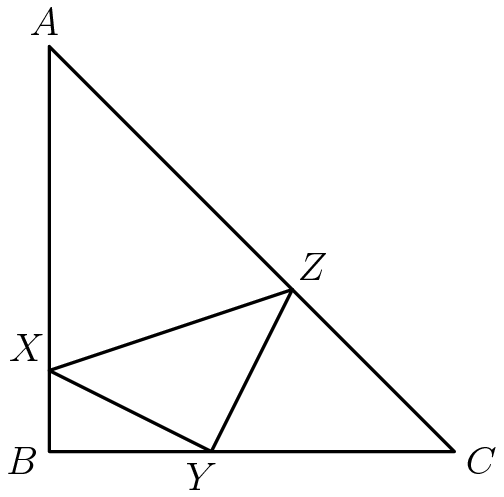
\includegraphics[width=7cm,height=7cm]{Sections/Files/O-matt-trianglemin.png}
	
	Let $\angle B$ be the right angle. If $Z$ is the right angle of $\triangle XYZ$, then we leave it as an exercise to the reader to show that the minimal 
	configuration happens when $\triangle XYZ$ is the medial triangle of $\triangle ABC$. However, there is another case: the right angle is on one of the legs. 
	Let $Y$ be the right angle; then let $\angle XYB = a$. Through some angle chasing, we find $\triangle AXZ \sim \triangle CZY$ with ratio $\sqrt{2}$. Letting $s$ be the leg length
	of $\triangle ABC$ and $x$ the leg length of $\triangle XYZ$ we have $$BY = x \cos(a) \iff YC = s - x \cos(a) \iff AZ = \sqrt{2}(s - x\cos(a))$$ and 
	$$BX = x\sin(a) \iff XA = s - x\sin(a) \iff CZ = \frac{s-x\sin(a)}{\sqrt{2}}$$ and so $$AZ + CZ = AC = s\sqrt{2} \iff s = x(2\cos(a) + \sin(a)).$$
	The maximum of $2\cos(a) + \sin(a)$ is $\sqrt{5}$ (use Cauchy-Schwarz or properties of combined sinusodial functions) so our minimum $x$ is $\frac{s}{\sqrt{5}}$
	and our minimum area is $\frac{[ABC]}{5} = \boxed{240}$.
	%Put sol here
\end{solution}\bigskip
	\newpage

	\subsubsection{Detente}
	\label{15.1.7}
	\SSbreak\\
\emph{Source: 2016 CMIMC N10}\\
\emph{Proposer: \Paiya}\\ %\Pchan \Pbrain \Pss
\emph{Problem ID: 210}\\
\emph{Date: 2021-06-13}\\
\emph{Difficulty: Challenging}\\
\SSbreak
 
\SSpsetQ{
    Let $$S = \sum_{n=1}^\infty \text{lcm}[n,69]^{-2}.$$ Find $\lfloor 10^9S \rfloor.$ \calculator

    \textit{Hint.} $\sum_{n=1}^\infty \text{lcm}[n,1]^{-2} = \frac{\pi^2}{6}.$
    %Put Problem Here
}\bigskip

\begin{solution}\hfil\medskip
	
    \href{http://cmimc-official.herokuapp.com/docs/past-tests/2016_NumberTheory_S.pdf}{Solution} Answer: \fbox{1303995}
    %Put sol here
\end{solution}\bigskip

	\newpage
    
    \ihead{\footnotesize\bfseries\sffamily{SALT-1 (Season 15), Week 2}}
    \subsection{Week 2}
    
    \subsubsection{Senior Math; What Challenge?}
	\label{15.2.1}
	\SSbreak\\
\emph{Source: 1998 SMC}\\
\emph{Proposer: \Pss}\\ %\Pchan \Pbrain \Pss
\emph{Problem ID: 211}\\
\emph{Date: 2021-06-14}\\
\emph{Difficulty: Beginner}\\
\SSbreak

\SSpsetQ{

A cube is inscribed in a sphere of diameter 1. What is the surface area of the cube? 
}\bigskip

\begin{solution}\hfil\medskip
  
    This means that the cube has space diagonal $1$, so $3s^2 = 1 \iff s^2 = \frac{1}{3} \iff SA = 6s^2.$ Answer: \fbox{4}
\end{solution}\bigskip

	\newpage

	\subsubsection{Prisoner's Stupid Dilemma}
	\label{15.2.2}
	\SSbreak\\
\emph{Source: Original}\\
\emph{Proposer: \Pbrain}\\ %\Pchan \Pbrain \Pss
\emph{Problem ID: 212}\\
\emph{Date: 2021-06-15}\\
\emph{Difficulty: Beginner}\\
\SSbreak

\SSpsetQ{
	There are 100 prisoners numbered 1 to 100, and 100 boxes also labelled 1 to 100. The boxes are kept inside a room and the numbers 1 to 100 are randomly placed inside each box (one number in each box, and each number appears exactly once). In sequence, each prisoner enters the room and is allowed to look inside 50 boxes. If they find their number, they are released and allowed to communicate with the next prisoners. Otherwise, all the prisoners are executed. 
If the prisoners play optimally, the probability they are all released is $p$. Find $\floor{1000p}$. \calculator
}\bigskip

\begin{solution}\hfil\medskip
	
	Suppose Brainy is the first prisoner. He clearly has no better strategy than random guessing, getting his number with probability $\frac{1}{2}$. 
	If he does get his number, then he should remember the numbers in the remaining 49 boxes that he opened and tell that to the remaining 99 prisoners.
	Then, each prisoner will either know which box to open (because Brainy opened the box with their number in it) or they will know 50 boxes that don't contain
	their number (Brainy doesn't mention their number, so of the 50 boxes he opened none of them contain their number). But this means that they can all
	successfully escape! Our answer is \fbox{500}.
	%Put sol here
\end{solution}\bigskip

	\newpage

	\subsubsection{Coordinates without Bash}
	\label{15.2.3}
	\SSbreak\\
\emph{Source: \Cop}\\
\emph{Proposer: \Plot}\\ %\Pchan \Pbrain \Pss
\emph{Problem ID: 213}\\
\emph{Date: 2021-06-16}\\
\emph{Difficulty: Easy}\\
\SSbreak

\SSpsetQ{

    There is a circle that goes through the points $(2+\sqrt{2}, 1-\sqrt{7})$ and $(5,1)$ with radius $3$. Let $(a,b)$ be the circle's center. Given $a+b$ is a positive integer, find $a^b+b^a$.
}\bigskip

\begin{solution}\hfil\medskip
  
    Notice that $\sqrt{2}^2+\sqrt{7}^2=3^2$, so we try and see that a circle centered at $(2,1)$ does go through $(2+\sqrt{2}, 1-\sqrt{7})$. Using the distance formula, we see it also goes through $(5,1)$. The other and only possible circle has its center reflected across the midpoint of the two given points. Since one point has lattice coordinates and the other is irrational, the midpoint must have irrational coordinates. Therefore, this other circle's center has irrational coordinates. Since $2$ and $7$ are relatively prime, it is impossible for the sum of the this center's coordinates to be an integer. Therefore the circle centered at $(2,1)$ is the only possible circle, giving us the answer of $2^1+1^2=\boxed{3}.\square$
\end{solution}\bigskip
	\newpage

	\subsubsection{WA Can't Solve This, Either}
	\label{15.2.4}
	\SSbreak\\
\emph{Source: 2013 HMMT A7}\\
\emph{Proposer: \Pchan}\\ %\Pchan \Pbrain \Pss
\emph{Problem ID: 214}\\
\emph{Date: 2021-06-17}\\
\emph{Difficulty: Medium}\\
\SSbreak

\SSpsetQ{

$$\sum_{k_1 = 0}^\infty \sum_{k_2 = 0}^\infty \cdots \sum_{k_8 = 0}^\infty \dfrac{k_1 + k_2 + \cdots + k_8}{5^{k_1 + k_2 + \cdots + k_8}} = \dfrac{m}{n},$$
where $m, n$ are relatively prime positive integers. Find the sum of positive divisors of $mn$.
\begin{center}
    \textit{(A scientific calculator may be used.)}
\end{center}
}\bigskip

\begin{solution}\hfil\medskip
  
    \href{https://hmmt-archive.s3.amazonaws.com/tournaments/2013/feb/alg/solutions.pdf}{Solution} Answer: \fbox{19199495335}
\end{solution}\bigskip

	\newpage

	\subsubsection{WA Can't Solve This, Either}
	\label{15.2.5}
	\SSbreak\\
\emph{Source: USAMTS Y19R1P3}\\
\emph{Proposer: \Paiya}\\ %\Pchan \Pbrain \Pss
\emph{Problem ID: 215}\\
\emph{Date: 2021-06-18}\\
\emph{Difficulty: Hard}\\
\SSbreak

\SSpsetQ{
Let $S$ be the set of all ordered triples of positive integers $(a, b, c)$ such that 
$$\arctan \dfrac{1}{a} + \arctan \dfrac{1}{b} + \arctan \dfrac{1}{c} = \dfrac{\pi}{4},$$
where the range of $\arctan(x)$ is $[-\pi/2, \pi/2].$ Find $$\sum_{(a, b, c) \in S} abc.$$
}\bigskip

\begin{solution}\hfil\medskip

\href{https://usamts.org/Solutions/Solution3_1_19.pdf}{Solution} Answer: \fbox{1293}
\end{solution}\bigskip

	\newpage

	\subsubsection{cHriS geO}
	\label{15.2.6}
	\SSbreak\\
\emph{Source: 2020 Iran MO R3G4}\\
\emph{Proposer: \Pchris}\\ %\Pchan \Pbrain \Pss
\emph{Problem ID: 216}\\
\emph{Date: 2021-06-19}\\
\emph{Difficulty: Challenging}\\
\SSbreak
 
\SSpsetQ{
    $\triangle PQR$ has $PQ = 6, QR = 7, RP = 8$, incentre $I$, and circumcentre $O$. The external angle bisector of $P$ meets $\overleftrightarrow{QR}$ at $S$, 
    and $I_Q$ is the $Q$-excentre. The point $T$ is chosen along $\overleftrightarrow{IQ}$ such that $QT = 2IQ$ and $IT > IQ.$ Let $F$ be the point on the circumcircle
    of $\triangle DI_QT$ such that $DF$ is a diameter. Then the perimeter of $\triangle OIF$ can be expressed in the form $\frac{a + b \sqrt{c}}{d}$,
    where $\gcd(a, b, d) = 1$, $a, b$ are integers, and $c, d$ are positive integers. Find $1000a + 100b + 10c + d.$
    %Put Problem Here
}\bigskip

\begin{solution}\hfil\medskip

    \href{https://artofproblemsolving.com/community/c6h2347106p18981757}{Solution} so $O, I, F$ are collinear; using $OI^2 = R^2 - 2Rr$ we get $IF = \frac{16 \sqrt{15}}{15} \iff \boxed{3530}.$
    %Put sol here
\end{solution}\bigskip

	\newpage

	\subsubsection{Treaty Violation}
	\label{15.2.7}
	\SSbreak\\
\emph{Source: chinese guy}\\
\emph{Proposer: \Paiya}\\ %\Pchan \Pbrain \Pss
\emph{Problem ID: 217}\\
\emph{Date: 2021-06-20}\\
\emph{Difficulty: Challenging}\\
\SSbreak

\SSpsetQ{

    Let $f: \mathbb{R}^{2020} \to \mathbb{R}$ be the function 
    $$f\left(a_1, a_2, \cdots , a_{2020}\right) = \dfrac{a_1^2 + a_2^2 + \cdots + a_{2020}^2 + \left(a_1 + a_2 + \cdots + a_{2020}\right)^2}{\sqrt{a_1^4 + a_2^4 + \cdots + a_{2020}^4 + \left(a_1 + a_2 + \cdots + a_{2020}\right)^4}}.$$
    Then the maximum of $f$ is $M$, and the minimum of $f$ is $m$. Find $\lfloor 10^9M + 10^6m \rfloor.$ \calculator
}\bigskip

\begin{solution}\hfil\medskip
  
    In fact, $f$ has the range $$\left[\sqrt{\dfrac{m(m-1)}{m^2-3m+3}}, \sqrt{\dfrac{m\left(m^2-1\right)}{m^2+3}}\,\right]$$ where $m = n + 1$, giving us an answer of \fbox{44956512067}. 
    The condition is equivalent to $a_1 + \cdots + a_m = 0$, where $m$ is odd. To find the minimum, WLOG $a_m$ be the largest term in absolute value (positive or negative) 
    then use C-S on $$a_1^2 + \cdots + a_{m-1}^2 = \left(a_1 + \cdots + a_{m-1}\right)^2 - 2 \sum_{i < j} a_ia_j = a_m^2 - 2 \sum_{i < j} a_ia_j$$ to arrive at 
    an answer. The end result is that we should maximize $a_m^2$ while minimizing $a_1^2 + \cdots a_{m-1}^2$. \medskip

    Unfortunately, the maximum is not so easy. Intuitively from QM-AM, the maximum should happen when the $a$'s are close together; in fact, the equality 
    case happens when there are $\lfloor m/2 \rfloor$ equal terms of one sign and $\lceil m/2 \rceil$ equal terms of the other. The proof of this is absolute 
    hell and involves 4 different inequalities (one that you have to make up yourself) and smoothing/mixing variables, so just trust that the fakesolve works.
\end{solution}\bigskip

	\newpage

\ihead{\footnotesize\bfseries\sffamily{Quality Control (Season 16)}}
\section{Quality Control (Season 16)}

    \ihead{\footnotesize\bfseries\sffamily{Quality Control (Season 16), Week 1}}
    \subsection{Week 1}

    \subsubsection{The Rare non-Troll NJOY Problem}
	\label{16.1.1}
	\SSbreak\\
\emph{Source: Unknown}\\
\emph{Proposer: \Pnjoy}\\ %\Pchan \Pbrain \Pss
\emph{Problem ID: 218}\\
\emph{Date: 2021-06-28}\\
\emph{Difficulty: Beginner}\\
\SSbreak

\SSpsetQ{

If $n^2\%$ of $n$ is 80, find $n$.
}\bigskip

\begin{solution}\hfil\medskip
  
    We have $$\frac{n^2}{100} \cdot n = 80 \iff n = \boxed{20}.$$
\end{solution}\bigskip

	\newpage

	\subsubsection{The Common Troll NJOY Problem}
	\label{16.1.2}
	\SSbreak\\
\emph{Source: 2017 Fall OMO \#4}\\
\emph{Proposer: \Pnjoy}\\ %\Pchan \Pbrain \Pss
\emph{Problem ID: 219}\\
\emph{Date: 2021-06-29}\\
\emph{Difficulty: Beginner}\\
\SSbreak

\SSpsetQ{

	Chris draws a line segment between each of the points
	$$A(4, 4), B(-4, 4), C(-4, -4), D(4, -4), E(2, 0), F(0, 2), G(-2, 0), H(0, -2)$$
	on a sheet of paper large enough so that none of the line segments touch the edge of the paper. 
	He wants to separate all the regions obtained by the line segments and later on eat them. \medskip

	What is the maximum number of regions of paper that Chris can eat?
}\bigskip

\begin{solution}\hfil\medskip
  
	Note that the diagram is diagonally symmetric, so we need only to look at the intersections 
	in the interior of $\triangle AOB$, where $O$ is the origin. Count that there are 15 intersections, 
	then multiply by 4 to get 60. However, the troll is that Chris is cutting out sections on a piece of paper, 
	so the outside of square $ABCD$ is also a region and our answer is \fbox{61}.

	\begin{center}
\includegraphics[width=7cm,height=7cm]{Sections/Files/16-1-2.png}\end{center}
\end{solution}\bigskip

	\newpage

	\subsubsection{Parallelogram PTSD}
	\label{16.1.3}
	\SSbreak\\
\emph{Source: Italian Team Competition}\\
\emph{Proposer: \Phobo}\\ %\Pchan \Pbrain \Pss
\emph{Problem ID: 220}\\
\emph{Date: 2021-06-30}\\
\emph{Difficulty: Medium}\\
\SSbreak

\SSpsetQ{
    Diagonals of parallelogram $NJSM$ interescts at $E$, angle bisectors of $\angle MNE$ and $\angle EJS$ intersects at $L$. Given that $MESL$ is a parallelogram and $\overline{NM}=35$, compute $\overline{NJ}^2$.
    %Put Problem Here
}\bigskip

\begin{solution}\hfil\medskip
	
    Note $NS\parallel ML$ so $\angle NLM=\angle LNE = \angle MNL$ which makes $\triangle MNL$ isosceles, hence $\overline{MN} = \overline{ML}=\overline{ES}$. With a similar reasoning we get $\triangle JSL$ isoceles, with $\overline{JS}=\overline{SL}=\overline{EM}$, but $\overline{MN}=\overline{JS}$ so $\overline{EM}=\overline{ES}$, but recalling $E$ is the midpoint of both diagonals, $\overline{NS}=\overline{JM}$, making $NJSM$ a rectangle. Now $\overline{MJ}=2\cdot\overline{MN}$, which gives $\overline{NJ}=\sqrt{3}\cdot \overline{NM}$, so finally $\overline{NJ}^2=3\cdot \overline{NM}^2=\boxed{3675}$.
    \begin{figure}[h!]
        \centering
    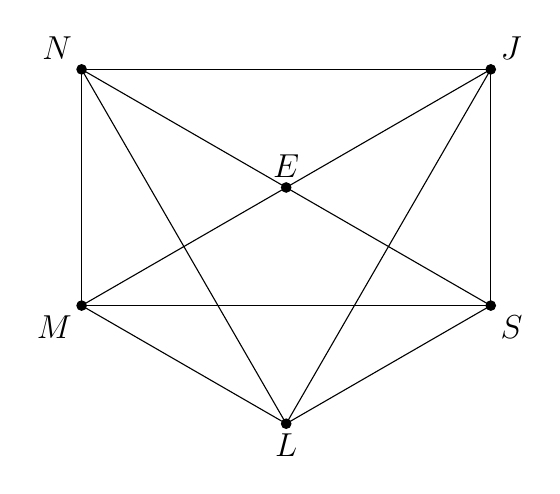
\begin{tikzpicture}[scale=3]
    \def\N{(0,1)};
    \def\J{(1.73205080757,1)};
    \def\S{(1.73205080757,0)};
    \def\M{(0,0)};
    \def\E{(0.86602540378,0.5)};
    \def\L{(0.86602540378,-0.5)};
    \draw \N -- \J -- \S -- \M -- \N;
    \draw \N -- \S -- \L -- \M -- \J -- \L -- \N;
    \filldraw \N circle (0.02) node[above left] {\large $N$};
    \filldraw \J circle (0.02) node[above right] {\large $J$};
    \filldraw \S circle (0.02) node[below right] {\large $S$};
    \filldraw \M circle (0.02) node[below left] {\large $M$};
    \filldraw \E circle (0.02) node[above] {\large $E$};
    \filldraw \L circle (0.02) node[below] {\large $L$};
    \end{tikzpicture}
    \end{figure}
    %Put sol here
\end{solution}\bigskip
	\newpage

	\subsubsection{WA Could Solve This and you Still Failed}
	\label{16.1.4}
	\SSbreak\\
\emph{Source: Original}\\
\emph{Proposer: \Paiya}\\ %\Pchan \Pbrain \Pss
\emph{Problem ID: 221}\\
\emph{Date: 2021-07-01}\\
\emph{Difficulty: Medium}\\
\SSbreak

\SSpsetQ{
    A real number $a$ is selected uniformly at random between $-50$ and $50$ inclusive. 
    The probability that $20x - \left|21x - \left|x + \frac{20a}{21}\right|\right| = 42|x - 1|$ has real solutions
    can be expressed in the form $\frac{m}{n}$, where $m$ and $n$ are relatively prime positive integers. 
    Find $100m + n$.
	%Put Problem Here
}\bigskip

\begin{solution}\hfil\medskip
	
    Let the LHS be $f(x)$. The graph of $f$ looks like a bunch of lines, and $f$ is continuous (why?). 
    The maximum absolute value of the slope of a line that's part of $f$ can be is $42$, which means that if $f$ crosses 
    the RHS then $f(1) \geq 0$, since $x = 1$ is where the minimum of $42|x-1|$ is attained; 
    if $f(1) < 0$ then $f$ will never cross $42|x-1|$. This is because for $f$ to cross $42|x-1|$ for $x < 1$ when $f(1) < 0$, 
    $f$ would have to somehow go from being above the V-shaped absolute value graph of $42|x-1|$ to below it at $x = 1$, impossible 
    since no part of $f$ has slope of absolute value greater than $42$; analogously we see that $f$ cannot cross $42|x-1|$ when $x > 1$. Solve to get 
    $-\frac{441}{10} \leq a \leq -\frac{21}{10}$ and $0 \leq a \leq 42$. Our probability is $\frac{21}{25} \iff \boxed{2125}.$
	%Put sol here
\end{solution}\bigskip

	\newpage


    
    \ihead{\footnotesize\bfseries\sffamily{Quality Control (Season 16), Week 2}}
    \subsection{Week 2}
    
    

\end{document}